%\documentclass[11pt,a4paper]{scrartcl}
%\documentclass[12pt,openright,twoside]{report} %,titlepage
\documentclass[12pt]{report}
%\usepackage[top=2.0cm, right=2.0cm, left=2.0cm, bottom=2.0cm]{geometry}
%\usepackage{setspace}
%\doublespacing
%\usepackage[left]{lineno}
%\linenumbers
\usepackage[utf8]{inputenc}
\usepackage[french]{babel}
%tableau
\usepackage{array, multirow}
%graphs
\usepackage{multicol}
\usepackage{url}
\usepackage{graphicx}
\usepackage{float, caption}
\usepackage{amsmath,amssymb,mathrsfs}
\usepackage{natbib}
%\usepackage{apalike}
\usepackage{graphicx}
\usepackage{color}
\usepackage{pgf}
\usepackage{tikz}
\usetikzlibrary{arrows,snakes,backgrounds,shapes}

%pour avoir la biblio avec nom d'auteur et année dans le texte
\bibpunct{(}{)}{;}{a}{,}{,}
%pour avoir les reference entre parenthese et en cas de ref multiple séparé par des ;
\sloppy 
%utiliser ca si latex trop exigeant en largeur ligne

\title{Ecologie et Evolution des maladies infectieuses aiguës : le cas
  de la grippe}

\author{Sébastien Ballesteros}

\date{}


\newlength{\plarg}
\setlength{\plarg}{14cm}
\newlength{\glarg}
\setlength{\glarg}{15cm}


\begin{document}

\begin{titlepage}
\thispagestyle{empty}
\noindent


\includegraphics[width=0.2\linewidth]{upmc.eps}

\begin{center}
\begin{minipage}{\plarg}
\centering
{\large\bfseries Thèse de doctorat de l'université Pierre et Marie Curie}\\ \vspace{0.4cm}
{\huge\bfseries Ecologie et Evolution des maladies infectieuses aiguës : le cas
  de la grippe }\\ \vspace{0.4cm}
Ecole doctorale Diversité du vivant\\ \vspace{1mm}
{\large\bfseries Spécialité Ecologie Evolution}\\ \vspace{0.4cm}
présenté par \\ \vspace{1mm}
{\large\bfseries Sébastien Ballesteros }\\ \vspace{0.4cm}
pour obtenir le grade de \\ \vspace{1mm}
{\large\bfseries DOCTEUR de l’UNIVERSITÉ PIERRE ET MARIE CURIE}\\ \vspace{0.4cm}
\end{minipage}
\end{center}

\noindent
soutenue le 18 décembre 2009 devant le jury composé de : \vspace{5mm}\\
M. van Baalen Minus, co-Directeur de thèse\\
M. Cazelles Bernard, Directeur de thèse\\
M. Fraser Christophe, Examinateur\\
Mme. Pontier Dominique, Rappporteur\\
M. Thomas Guy, Président du Jury\\
Mme. Vergu Elisabeta, Examinateur\\
Mme. Viboud Cécile, Rappporteur\\


\vspace{0.4cm}

%{\rule{\plarg}{1pt}} \vspace{3mm}
%\begin{tabular}{p{5cm}p{5cm}p{4cm}}
%\vfill AA & \vfill Professeur  & \vfill Directeur \\
%BB & Maître de Conférences & Rapporteur \\
%etc \dots & &
%\end{tabular}



\vfill \hspace{-1cm}
\begin{minipage}{\glarg}
{\rule{\glarg}{1pt}}
\begin{tiny}
  Université Pierre \& Marie Curie - Paris 6 \hfill Tél. Secrétariat : 01 42 34 68 35\\
  Bureau d’accueil, inscription des \hfill  Fax : 01 42 34 68 40\\
  doctorants et base de données \hfill Tél. pour les étudiants de A à EL : 01 42 34 69 54\\
  Esc G, 2ème étage \hfill Tél. pour les étudiants de EM à MON : 01 42 34 68 41\\
  15 rue de l’école de médecine \hfill  Tél. pour les étudiants de MOO à Z : 01 42 34 68 51\\
  75270-PARIS CEDEX 06 \hfill E-mail : scolarite.doctorat@upmc.fr
\end{tiny}
\end{minipage}



\end{titlepage}



%%% Local Variables: 
%%% mode: latex
%%% TeX-master: "phD"
%%% End: 

\newpage
\thispagestyle{empty}
\null
\newpage

\maketitle

%ne surtout pas utiliser %\abstract{} !!!
%fou la merde !!!


\begin{quote}
  (history) is itself a Western invention whose central theme is the
  rejection of habitat. It formulates experience outside of nature and
  tends to reduce place to location... It seeks causality in the
  conscious, spiritual, ambitious character of men and memorializes
  them in writing.\\
  \textsc{Paul Shepard}
\end{quote}

\cleardoublepage

\section*{Résumé}

Cette thèse s'intéresse aux interactions entre immunologie,
épidémiologie et biologie évolutive. Nous utilisons une combinaison
d'approches mathématiques et statistiques pour comprendre les
processus gouvernant les dynamiques épidémiologiques et les
phylogénies observées pour différents pathogènes de l'échelle
individuelle aux populations. Nous prenons l'exemple de la grippe
humaine. Trois hypothèses permettent de rendre compte de la
phylodynamique particulière de la grippe: (i) il existe un mécanisme
de densité-dépendance directe médié par une période temporaire
d'immunité totale après infection ; (ii) le nombre de phénotypes
possibles est limité, les virus les ré-explorant sans cesse ; (iii)
l'évolution de l'antigène principal de la grippe est ponctuée, les
échappements ponctuels à l'immunité induisant des balayages
sélectifs. (iii) domine aujourd'hui et rend compte de la variabilité
des épidémies de grippe, de larges échappements à l'immunité en
induisant de plus grandes. Nous montrons que le formalisme ayant mené
à (iii) induit de manière implicite un processus immunologique
irréaliste pour la grippe. Nous révélons que les séries temporelles
d'incidences grippales ne peuvent pas fournir une preuve du caractère
ponctué de l'évolution antigénique, un modèle parcimonieux prenant en
compte une évolution antigénique purement graduelle les
reproduisant. La nature chaotique de ces dynamiques marque une limite
fondamentale à la prédictibilité de la taille des épidémies de grippe
et ce, indépendamment de la contingence évolutive. Nous développons un
formalisme confrontable aux données pour tester les différentes
hypothèses rendant compte de la phylodynamique de la grippe.



\vspace{2cm}

{\noindent
\textbf{Mots clés} : écologie ; évolution ; épidémiologie ; grippe ;
modèles multi-souches ; système immunitaire ; système dynamique ;
dynamique chaotique ; phylodynamique ; filtrage particulaire
}


\clearpage

My thesis focuses on the melding of immunodynamics, epidemiology and
evolutionary biology. I use a combination of mathematical and
statistical approaches to understand the processes driving outbreak
dynamics and the wide range of pathogen phylogenies observed at scales
from individual host to populations. I mostly focus on human influenza
A. Three hypothesis have been proposed to explain the distinctive
phylodynamic pattern observed in human influenza viruses: (i) that
there is short-lived cross-immunity among viral strains acting as a
direct density-dependent process that restricts strains diversity;
(ii) that the virus continually reuses a limited number of antigenic
combinations; (iii) that influenza A main antigen (hemagglutinin)
evolves in a punctuated manner, punctuated immune escape resulting in
selective sweeps. This latter hypothesis is currently widely accepted
and enables to explain influenza epidemics peaks variability, higher
peaks reflecting higher punctual antigenic changes. We first show that
hypothesis (iii) implicitly induces an irrealistic immunological
process in the context of influenza. We then revealed that influenza
incidence time-series cannot constitute a proof of punctuated
antigenic evolution as a parsimonious model considering only purely
gradual antigenic drift successfully reproduces the data. The chaotic
nature of these dynamics sets fundamental limits to the predictability
of future epidemics sizes in addition to evolutionary
contingency. Last, we develop a framework suitable to statistical
analysis in order to disentangle the various processes shaping
influenza phylodynamics.






\cleardoublepage
%\newpage
%
\section*{Remerciements}
\label{sec:thanks}

Experienced misanthrope and proud to be so.


%%% Local Variables: 
%%% mode: latex
%%% TeX-master: "../phD"
%%% End: 

%\clearpage

\tableofcontents


%\begin{quote}
%  Chaque histoire s'accompagne d'un nombre indéterminé d'anti-histoires dont chacune est complémentaire des autres.\\
%  \textsc{Claude Lévi-Strauss}
%\end{quote}

%\cleardoublepage
\clearpage
\newpage
\thispagestyle{empty}
\null
\newpage

 
\chapter{Introduction}
\label{sec:intro}

%voir aussi quotation

Cette thèse porte très largement sur la grippe. Cependant, étant donné
le nombre considérable d'excellentes synthèses sur ce sujet par
exemple (\citet{Webster1992} ; \citet{Earn2002} ; \citet{Cox2000a} ;
\citet{Nelson2007}) nous avons préféré resituer la grippe dans le
contexte globale des maladies infectieuses humaines, en cherchant à
comprendre comment facteurs écologiques et évolutifs ont pu façonner
la grippe humaine. Nous avons néanmoins essayé d'introduire
progressivement dans le texte les notions clefs associées à la grippe,
mais le lecteur souhaitant une approche plus structurée sur ce seul
sujet gagnera à consulter les synthèses précédemment citées.

\section{Origine des principales maladies infectieuses humaines: les
  transitions épidémiologiques}


\subsection{Première transition: la révolution néolithique}


%Dans son essais ``The Worst Mistake In The History Of The Human Race''
%datant de 1967, Jared Diamond concluait:
%
%``Suppose that an archaeologist who had visited us from outer space
%where trying to explain human history to his fellow spacelings. He
%might illustrate the results of his digs by a twenty-four hour clock
%on which one hour represents 100,000 years of real past time. It the
%history of the human race began at midnight, then we would now be
%almost at the end of our first day. We lived as hunter-gatherers for
%nearly the whole of that day,from midnight through dawn, noon, and
%sunset. Finally, at 11:54 p.m., we adopted agriculture. As our second
%midnight approaches, will the plight of famine-stricken peasants
%gradually spread to engulf us all? Or will we somehow achieve those
%seductive blessings that we imagine behind agriculture's glittering
%facade and that have so far eluded us?''

La révolution néolithique il y a environ 11 000 ans a constitué un
tournant majeur dans l'histoire de l'humanité. Le changement d'un mode
de vie essentiellement nomade de type ``chasseur-cueilleur'' marqué
par de petites tailles de population à un mode de vie sédentaire
centré autour de la pratique agricole et la domestication animale et
végétale a constitué sans doute le bouleversement le plus conséquent
que notre espèce ait traversé. Les débuts de l'agriculture ont dû être
particulièrement éprouvants pour les premières sociétés agricoles. Les
études paléopathologiques comparant les squelettes des sociétés pré et
post agricoles révèlent en effet que les premiers agriculteurs étaient
plus petits et avaient une espérance de vie considérablement réduite
par rapport aux chasseurs ceuilleurs avoisinants. Les premiers
agriculteurs étaient généralement moins bien nourris et plus exposés
aux maladies infectieuses \citep{McMichael2004}.

L'exposition accrue aux maladies infectieuses résulte de plusieurs
facteurs. La sédentarisation a par exemple confronté davantage les
communautés humaines à leurs propres déchets favorisant un contact
accru avec de nombreux parasites et la prolifération d'insectes et de
rongeurs. Cependant le facteur majeur semble avoir été la
domestication animale et les contacts considérablement plus fréquents
entre humains et animaux domestiques \citep{Diamond2002}. Ces contacts
accrus ont grandement favorisé la probabilité que des pathogènes
adaptés aux animaux franchissent la barrière d'espèces
\citep{Antia2003} et s'introduisent dans la nouvelle niche écologique
offerte par une population humaine grandissante. Le développement des
premières villes marquées par de fortes densités de populations
humaines a constitué le facteur associé conduisant à l'établissement
durable de ces nouveaux agents infectieux \citep{Armelagos2005}. Les
études sur la rougeole sont particulièrement illustratrices à ce
sujet. La rougeole comme l'essentiel des maladies infectieuses aiguës
provoque une infection relativement courte de l'ordre de grandeur de
la semaine résultant en une épidémie explosive. Du fait de la
déplétion du stock de susceptibles, la rougeole ne peut se maintenir
dans les petites communautés que si elle est réintroduite après que de
nouveaux individus immunologiquement naifs aient vu le jour. Les îles
Faroe d'une population de 25000 habitants ont fourni un exemple
saisissant de ce phénomène donnant lieu à des dynamiques critiques
suivant des lois puissance \citep{Rhodes1996, Rhodes1997}. Cependant,
comme le démontre \citet{Bartlett1957, Bartlett1960} à partir d'une
taille de communauté critique (CCS) (estimée de l'ordre de 250 000 -
500 000 individus pour la rougeole), le renouveau de susceptibles, du
fait des naissances et des morts, devient suffisant pour maintenir à
l'état endémique un agent infectieux provoquant une maladie aiguë.
\citet{Grenfell2001} montrent par exemple comment les grands centres
de population du royaume unis réensemencent les villes de tailles
inférieures à la CCS, permettant ainsi le maintien de la rougeole.

Des tailles de populations humaines de 250 000 - 500 000 habitant
n'existaient pas sur Terre avant l'émergence des villes et des
civilisation agricoles \citep{Diamond1999}. \citet{Black1975} a par
exemple montré que les populations amérindiennes isolées ayant gardé
le mode de vie chasseur cueilleur n'étaient pas soumises à ces
maladies aiguës. Ces communautés de l'ordre de grandeur de 300
personnes sont en effet trop réduites pour permettre le maintien des
maladies aigues. Elles étaient par contre sujettes à des maladies
chroniques, restant longtemps chez les hôtes ou bien réactivables
telle la varicelle.

Si la croissance marquée de la population humaine a offert de
nouvelles possibilités aux maladies infectieuses préexistantes, la
domestication animale et végétale et la présence grandissante de
grands troupeaux et peuplements végétaux cultivés a aussi fourni de
nouvelles niches écologiques à de nombreux organismes.
\citet{Mira2006} montrent par exemple que la révolution néolithique a
été accompagnée par une explosion du nombre de séquences d'insertion
dans les génomes bactériens associés aux larges communautés humaines
et agricoles. Ces séquences d'insertion sont supposées avoir participé
au processus de réduction génomique allant de pair avec une
spécialisation accrue aux nouvelles niches écologiques fournies par la
domestication.

\subsection{Seconde et troisième transition: contact entre les
  civilisations et décimations trans-océaniques}

L'origine des principales maladies humaines aiguës, les ``crowd
diseases'', est donc intimement liée à l'essor des civilisations
agricoles. Étant données les inégalités géographiques du potentiel de
domestication, ces maladies ont donc été longtemps associées aux
grands foyers de domestications animales situés essentiellement dans
l'Ancien Monde notamment en Eurasie (par exemple, 13 des 14
principales espèces de mammifères domestiques sont originaires
d'Eurasie) \citep{Diamond2002}. \citet{Wolfe2007a} montrent ainsi que
les régions tropicales ont plus souvent fourni des maladies
infectieuses chroniques, à plus longues périodes d'infections. Les
principales maladies infectieuses humaines venant de la zone tropicale
proviennent aussi en majorité de l'Ancien Monde. \citet{Wolfe2007a}
relient ce fait remarquable à l'importance qu'ont joué les primates
dans l'émergence des maladies infectieuses humaines (avec une
contribution d'environ 20 \% des principales maladies infectieuses
humaines). L'importance des primates s'explique par leur proximité
génétique avec l'homme favorisant le saut de barrière d'espèce. La
différence entre Ancien Monde et Nouveau Monde tropical se comprend
alors du fait que la distance génétique entre les humains et les
singes du Nouveau Monde est presque le double de celle séparant les
humains des singes de l'Ancien Monde et plusieurs fois supérieure à
celle séparant humains et grands singes de l'Ancien Monde.

Ainsi, si la seconde transition épidémiologique a constitué un échange
de maladies infectieuses au sein de l'Ancien Monde, la troisième
transition et le contact entre Ancien et Nouveau Monde a été plutôt un
processus de dissémination des nouvelles maladies dans des populations
jusqu'alors naïves. Plus que les conquistadors, l'arrivée de la
variole, de la rougeole et de la grippe suivies un siècle plus tard de
la malaria eurent raison de 90\% de la population native du nouveau
monde \citep{McMichael2001}. L'esclavagisme a été une composante
importante de cette introduction de maladies dans le Nouveau Monde.
Par exemple si l'origine de la dengue se trouve dans les forêts
d'Afrique ou d'Asie, elle fût décrite pour la première fois à
Philadephie en 1789 suite à l'import d'esclaves infectés et du vecteur
en Amérique \citep{Holmes2008}. De même, la fièvre jaune accompagna
les esclaves d'Afrique vers l'Amérique \citep{Bryant2007}.

\subsection{Quatrième  transition: le monde moderne à travers
  l'exemple de la grippe}

%%William H. Stewart, responsable de la santé publique des USA déclara
%%``Il est temps de refermer le livre des maladies infèctieuses,
%%d'annoncer que la guerre contre les pestilence a été gagné et de
%%basculer les ressources nationales vers des problèmes chroniques tels
%%que le cancer et les maladies cardio-vasculaires.''
%%L'optimisme des années 1970 fut cependant rapidement 

Dans une étude récente menée à l'échelle planétaire, \citet{Jones2008}
ont rigoureusement démontré un accroissement statistiquement
significatif du nombre d'évènements de maladies infectieuses
émergentes (corrigé de l'augmentation du taux de report) entre 1940 et
2004 avec un pic dans les années 1980 lors de la pandémie du SIDA. Ces
maladies infectieuses émergentes (EID) sont dûes à l'apparition de
nouvelles maladies chez l'homme (\textit{e.g} VIH, SRAS), à
l'apparition de formes résistantes de pathogènes (\textit{e.g}
Mycobacterium tuberculosis multirésistants, en raison de sa résistance
à au moins deux des principaux antituberculeux, résistance de
Plasmodium falciparum à l'antipaludique le plus utilisé, la
chloroquine) ou bien enfin à l'augmentation d'incidence de maladies
jusqu'alors peu prévalentes (\textit{e.g} maladie de Lyme).
\citet{Jones2008} révèlent en particulier la part prépondérante et le
nombre croissant des EID dûes à des zoonoses (60.3\% des 335 EID
reportées ) dont la majorité (71.8\%) trouvent leur origine chez les
animaux sauvages. \citet{Jones2008} proposent une carte des
``hotspots'' d'EID correspondant pour les zoonoses, aux régions avec
des changements démographiques récents et rapides, une production
animale en intensification ou récemment intensifiée et où la
biodiversité est élevée. Comme le rappellent ces auteurs en conclusion
de leur article, la conservation des zones riches en biodiversité
permet entre autre d'y réduire les activités anthropiques et par la
même de diminuer la probabilité d'émergence de futures zoonoses.

Il est en réalité possible de trouver une cause écologique directe
pour pratiquement toutes les maladies émergentes humaines modernes
\citep{Schrag1995, Morse1995}. En particulier on peut citer comme
facteurs invoqués, les changements de pratiques agricoles et d'usage
des sols tels l'intensification agricole et la déforestation,
l'explosion des capacités de transports et des flux de passagers,
l'urbanisation grandissante et l'essor des mégalopoles,
l'accroissement grandissant des inégalités sociales et de la densité
de population, le collapse des systèmes de santé publiques et
l'utilisation à grande échelle de médicaments favorisant l'apparition
de résistances (voir \citet{Daszak2000, Morens2004, Daszak2004,
  Woolhouse2005, Despommier2006} pour des synthèses). Si certains de
ces facteurs existent depuis très longtemps, la complexité du monde
actuel rend leurs actions plus effectives que jamais
\citep{Morens2008}.

Nous nous limiterons ici à l'exemple de la grippe dont la pandémie
actuelle \citep{Team2009} illustre plus que jamais l'actualité.  La
grippe humaine est provoquée par trois types antigéniques de virus
appartenant à la famille des Orthomyxoviridae, les virus grippaux A,
B, C par ordre de dangerosité décroissante pour notre espèce.

La grippe de type A est elle même divisée en différents sous-types
déterminés par les deux antigènes de surface majeure: l'hémagglutinine
(HA) et la neuraminidase (NA). Ces virus sont dispersés dans tout le
monde animal (oiseaux terrestres et marins, chevaux, porcs, mammifères
marins) mais sont originaires des oiseaux sauvages aquatiques et
notamment des canards sauvages qui constituent leurs réservoirs
naturels \citep{Webster1992}. On a identifié chez eux la totalité des
16 HA et 9 NA connus dont 103 des 144 combinaisons possibles
\citep{Dugan2008}. Les virus aviaires sont en outre différenciés selon
leur pathogénicité envers les poulets. Les souches causant des
épidémies sévères et de hauts taux de mortalité sont qualifiés de
virus aviaires hautement pathogènes (HPAI) tandis que ceux causant des
épidémies plus faibles chez les volailles domestiques sont classifiés
de virus aviaires faiblement pathogènes (LPAI) \citep{Olsen2006}.

\begin{figure}[!htbp]
  \begin{center}
    
\includegraphics[width=0.7\linewidth]{graphs/intro/ac.eps}
  \end{center}
  \caption{Spécificité des anticorps produits après vaccination de
    volontaires avec un vaccin contre la grippe saisonnière (reproduit
    d'après \citet{Wrammert2008}). On constate en particulier que 60\%
    des anticorps réactifs à la grippe sont dirigés contre HA.}
  \label{fig:1:ac}
\end{figure}

Les pandémies grippales humaines proviennent du passage de virus
aviaires complet ou seulement de certains gènes d'origine aviaire
et/ou porcin chez l'homme \citep{Zimmer2009}. Ce processus est
facilité par la nature fragmentée du génome de la grippe comprenant 8
brins d'ARN monocaténaire de polarité négative. La
figure~\ref{fig:1:legacy} récapitule l'histoire des pandémies récentes
depuis 1918 mettant en avant l'histoire génétique intriquée se
déroulant chez les hommes et les porcs depuis la grippe espagnole.
Cette grippe, datée de 1918 est responsable d'environ 4 fois plus de
morts que la première guerre mondiale et marque l'entrée dans la
population humaine de H1N1. Il est maintenant reconnu que cette grippe
est passée directement des oiseaux à l'homme très probablement en
raison des circonstances exceptionnelles associées à la première
guerre mondiale. En particulier, \citet{Oxford2005} suggèrent que son
origine pourrait remonter à 1916 au sein du camp militaire britannique
d'Etaples dans le nord de la France. Ce camp militaire ayant connu des
épidémies similaires à celle de 1918 présente en effet une conjonction
de facteurs remarquables avec plus de 100 000 soldats, sans cesse
renouvelés par l'arrivée quotidienne jour et nuit de trains déversant
des soldats blessés provenant des champs de bataille de la Somme ; un
logis surpeuplé fait de tentes et de baraquements temporaires en bois,
idéal pour la propagation d'une maladie respiratoire ; l'existence
d'une importante porcherie et la proximité de nombreux élevages et
marchés de poulets, canards oies et chevaux, le tout dans un milieu
hostile lourdement contaminé par la présence de 24 gaz (dont certains
mutagènes et irritants des voix respiratoires) créés par les combats.
Le déclenchement final aurait été le retour des millions de soldats
partout à travers le monde à l'automne 1918. De manière quasiment
simultanée un virus relativement similaire a fait son apparition chez
le porc en Amérique du Nord causant de nombreuses épidémies dans les
élevages \citep{Zimmer2009}. Depuis se déroule une histoire génétique
complexe, marquée par l'intrusion de nouveaux gènes d'origine aviaire
chez les hommes (H2N2 en 1957 et H3N2 en 1968) et les cochons (H1N1
porcin européen en 1979) \citep{Morens2009}. Cette introduction de
gènes se fait par réassortiment, nécessitant la coinfection par deux
types distincts de virus. Les réassortiments entre différents
sous-types peuvent être facilités par le porc, qui constitue un hôte
privilégié, sensible à la fois aux virus aviaires et humains
\citep{Webster1992}.

Ce mécanisme s'est répété récemment avec un triple réassortiment
(figure~\ref{fig:1:legacy}) ayant donné naissance à une nouvelle
souche de H1N1 pandémique apparue initialement dans la ville mexicaine
de La Gloria à la mi Février 2009 \citep{Fraser2009}. On peut
remarquer que cette région de l'état de Veracruz correspond à un des
hotspot d'EID de \citet{Jones2008}. D'une manière préoccupante, cette
souche, maintenant répandue à travers le monde, à été caractérisée
comme étant plus virulente que la grippe H1N1 saisonnière chez 3
modèles animaux (souris, furet et singes) \citep{Itoh2009}.

Les contacts répétés entre les hommes et les oiseaux aquatiques
sauvages, les volailles domestiques et les porcs (eux même en contact
avec les oiseaux aquatiques sauvages) sont donc la cause ultime de
l'apparition de nouvelles souches pandémiques chez l'homme. Ainsi,
\citet{Day2006} montrent que si les pandémies des 250 dernières années
ont eu lieu majoritairement via les réassortiments chez l'homme, alors
des milliers d'infections humaines par des virus aviaires doivent
avoir lieu chaque année. Ces auteurs montrent aussi que s'il existe
une diversité génétique importante chez les virus aviaires, la
multiplication des contacts entre hommes et animaux est le facteur
ayant le plus d'impact sur l'augmentation de la probabilité
d'apparition d'une pandémie dans la population humaine. Dans le
contexte de la quatrième transition épidémiologique décrite dans cette
partie, ces résultats sont particulièrement inquiétants car jamais les
contacts entre humains et animaux porteurs de la grippe n'ont été
aussi élevés \citep{Kapan2006, Leibler2009}.

L'augmentation sans précédent des productions animales avicoles et
porcines, en particulier dans des régions fortement peuplées et riches
en avifaune sauvage, est une cause directe de cette augmentation en
jouant le rôle d'un pont entre oiseaux sauvages réservoirs et
populations humaines mais aussi en ayant un impact direct sur
l'évolution des pathogènes. Ces deux points sont particulièrement bien
illustrés par l'épidémie de grippe aviaire H5N1 initialement reconnue
à Hong Kong en 1997 et caractérisée par son exceptionnel virulence
\citep{Jong2006}. La transition de virus LPAI à HPAI (pouvant être
provoquée par une seule mutation ponctuelle de HA) est en effet
largement favorisée par les conditions régnant dans les élevages
industriels à production intensive. Ces derniers sont en particulier
caractérisés par de très fortes densités d'animaux confinés et souvent
immunodéprimés où le renouvellement des susceptibles est de plus en
plus rapide dû d'une part à l'abattage de plus en plus précoce permis
par la sélection d'animaux à croissance rapide et d'autre part aux
nombreux échanges entre les fermes favorisant une dissémination rapide
avant que l'épidémie ne s'éteigne localement \citep{Leibler2009}.
\citet{Chen2006} révèle ainsi que les taux de substitution et les
pressions de sélection (mesurées par le ratio de substitutions non
synonymes sur synonymes) sont plus élevés chez les espèces domestiques
que chez l'ensemble des oiseaux sauvages.

A terme, seule une approche d'écologie de la santé \citep{Daszak2004,
  Wilcox2005, Kapan2006} permettra de gérer globalement les risques de
pandémies hautement virulentes grippales. \citet{Kilpatrick2006} ont
par exemple montré comment la diffusion de l'épizootie de grippe
aviaire H5N1 avait été le fait d'une synergie entre les mouvements
d'oiseaux migrateurs et le commerce international de volailles et
d'oiseaux sauvages. La diminution des contacts entre oiseaux
migrateurs venant nicher dans les zones agricoles et volailles
domestiques se fera par exemple de façon durable en restaurant les
zones humides, habitat naturel des oiseaux migrateurs aquatiques,
ayant été essentiellement détruites suite à l'extension des zones
agricoles irriguées \citep{Lemly2000}. Une approche d'écologie de la
santé à la grippe aviaire est d'autant plus souhaitable que la
situation actuelle a des répercussions à de multiples échelles.
\citet{Jeffries2004} ont par exemple montré que l'intensification de
l'agriculture a fourni un apport alimentaire aux Anatidae (cygnes,
oies, canards) qui a permis une croissance géométrique de leur
population. Ces grands nombres d'oiseaux ont drastiquement affecté les
marais côtiers de l'Arctique (où ils se reproduisent) affectant
négativement différents groupes d'organismes.


\begin{figure}[!htbp]
  \begin{center}
    \includegraphics[width=1\linewidth]{graphs/intro/legacy.eps}
  \end{center}
  \caption{Relation génétique entre les virus aviaires, humains et
    porcins pour la grippe A de 1918 à 2009 (reproduit d'après
    \citet{Morens2009}).}
  \label{fig:1:legacy}
\end{figure}


% Le traitement sur le long terme de la grippe ainsi que des EID devra
% donc faire appel à une approche

\clearpage


\section{Évolution des maladies infectieuses à travers différentes
  échelles spatio-temporelles}


Nous avons vu que l'accroissement des tailles de populations humaines
et de leurs plantes et animaux domestiques suite à la révolution
néolithique a induit un changement de pression de sélection majeur et
permis l'émergence de nouvelles formes d'agents infectieux.


\subsection{Différentes trajectoires évolutives}

Suite à ces changement écologiques et évolutifs majeurs, nous vivons
donc en présence de trois grands types de maladies:

\begin{itemize}
\item Des maladies aiguës très contagieuses et fortement immunisantes:
  l'âge de première infection est typiquement bas \citep{Anderson1992}
  et la protection acquise reste efficace à vie. Ce type de maladies
  constitue l'essentiel des maladies infectieuses infantiles.
\item Des maladies aiguës un peu moins transmissibles, résultant en un
  âge de première infection plus élevé et des réinfections tout au
  long de la vie. La grippe est l'exemple typique de cette catégorie.
\item Des maladies chroniques, largement moins transmissibles en
  moyenne, et marquées par des durées d'infections considérablement
  plus longues. Les maladies sexuellement transmissibles (dont le VIH)
  sont l'archétype de cette dernière catégorie.
\end{itemize}


%mettre exemple de dynamique

\subsection{Contraintes écologiques}

%%%%%%premiere approche purement écologique

Relativement peu d'études se sont intéressées aux trajectoires
évolutives pouvant mener aux maladies aiguës.  Pourtant, ce cas est
emblématique de la révolution néolithique et il existe des exemples
bien documentés. Le genre bactérien \textit{Bordetella} est
particulièrement illustratif avec 2 espèces, \textit{Bordetella
  pertussis} et \textit{Bordetella parapertussis} responsable de la
coqueluche, une maladie infantile aiguë humaine, ayant évoluée
indépendemment à partir de \textit{Bordetella bronchiseptica}, qui
infecte une large variété de mammifères sauvages et domestiques
généralement sous la forme d'une infection chronique et largement
avirulente \citep{Bjoernstad2005}.

Le modèle déterministe $SIR$ constitue un bon point de départ pour
l'étude de l'évolution des maladies infectieuses
\citep{Dieckmann2002}.  Par exemple, l'équation~\eqref{eq:intro_sir}
décrit un système ou 2 souches, référencées 1 et 2, sont en
compétition directe pour une même population d'hôtes susceptibles
($S$).

\begin{align}
  \label{eq:intro_sir}
  \dot{S} &= B -\beta_1SI_1 -\beta_2SI_2 -\mu R \\
  \dot{I_1} &= \beta_1SI_1 -\nu_1 I_1 -\alpha_1 I_1 -\mu I_1 \notag \\
  \dot{I_2} &= \beta_2SI_2 -\nu_2 I_2 -\alpha_2 I_2 -\mu I_2 \notag \\
  \dot{R} &= \nu_1 I_1 -\nu_2 I_2 -\mu R \notag
\end{align}

Dans ce système, $I_1$ et $I_2$ représentent la densité d'individus
infectés et infectieux pour les souches 1 et 2, $R$, la densité
d'individus guéris et immunisés. La population est soumise à des
naissances ($B$) et des morts selon un taux $\mu$. Les autres
paramètres décrivent le taux de guérison, $\nu$, qui détermine le
temps d'infection ($1/ \nu$), le taux de transmission, $\beta$, et la
virulence de l'agent infectieux, $\alpha$, mesuré comme l'extra
mortalité qu'il induit.

On peut montrer que sous ce système, l'agent infectieux ayant le plus
grand taux de reproduction de base ($R_0$ défini comme le nombre
d'infections secondaires provoquées par un individu infecté placé dans
une population totalement susceptible $R_0=\frac{\beta}{\mu + \nu
  +\alpha}$) l'emporte et exclut compétitivement l'autre souche.

Le modèle $SIR$ déterministe prédit ainsi une évolution maximisant le
$R_0$ et donc une évolution vers un taux de guérison et une virulence
les plus petits possibles, menant vers des maladies chroniques
avirulentes.

\citet{Ballegooijen2004} ont été parmi les premiers à proposer un
mécanisme capable d'expliquer une évolution vers des maladies aiguës.
Ces auteurs ont considéré comme base de leur étude un modèle $SIRS$
sous la forme d'un automate cellulaire. Ce modèle permet un retour des
individus immunisés ($R$) vers l'état susceptible $S$ (suite à une
immunité décroissante ou une évolution antigénique de l'agent
infectieux) et tient compte de la structuration spatiale de la
population d'hôtes (sur une grille en deux dimensions). Dans ce
contexte spatial \citet{Ballegooijen2004} montrent qu'un compromis
évolutif linéaire entre taux de guérison et taux de transmission
émerge. Le système évolue de lui même vers une valeur de $R_0$ puis
cette valeur restant constante, la durée d'infection diminue. Cette
sélection pour des maladies aiguës s'explique par le fait que les
agents infectieux à courte durée d'infection induisent des vagues
épidémiques plus fréquentes. L'auto-organisation spatiale du système
conduit donc, en l'absence de contraintes physiologiques, à une
sélection pour la fréquence des épidémies.

\citet{Read2007} ont montré que l'évolution vers des maladies aiguës
pouvait aussi avoir lieu en considérant le modèle $SIR$ de
l'équation~\eqref{eq:intro_sir} (et donc sous l'hypothèse de la loi
d'action de masse où la population est parfaitement mélangée) où
différentes souches sont en compétition directe pour la même
ressource, mais en tenant compte de la stochasticité démographique. En
imposant un $R_0$ constant, et donc en imposant un compromis évolutif
linéaire entre transmission et taux de guérison, \citet{Read2007}
révèlent l'existence d'une instabilité évolutive à partir de laquelle
deux trajectoires évolutives sont possibles, l'une menant vers des
maladies aiguës et l'autre vers de longues durées d'infections. Au
coeur de ce mécanisme se trouve un compromis évolutif à deux échelles
temporelles entre capacité d'invasion et capacité à persister
\citep{Keeling2000}. A $R_0$ identique, les agents infectieux évoluant
vers de courtes durées d'infection génèrent des épidémies plus rapides
mais avec un risque d'extinction post-épidémique considérablement
accru. En considérant que les agents infectieux peuvent être
réintroduits, \citet{Read2007} ont observé deux régimes distincts:
dans le cas où le système évolue vers des agents infectieux à courte
durée d'infection, on observe de rapides épidémies explosives
résultant en de fréquentes extinctions. Pendant ces périodes
d'extinction, le stock de susceptibles se renouvelle grâce au
processus démographique et la présence de réintroduction peut générer
de nouvelles épidémies. Lorsque différentes souches sont
réintroduites, les souches capables d'infecter rapidement le plus
grand nombre d'hôtes sont avantagées, et ainsi, on observe une
sélection vers des souches de plus en plus aiguës. Une conséquence de
cette dynamique de type ``boom and bust'' est l'apparition d'une
covariance fortement négative entre le nombre de susceptibles et
d'infectés, ce qui, comme montré par \citet{Keeling2000} a le même
effet que de diminuer le $R_0$. A l'inverse, dans le régime où les
agents infectieux évoluent vers de longues durées d'infections, le
nombre de susceptibles et d'infectés est beaucoup plus proche de celui
correspondant à l'équilibre déterministe et il y a donc une covariance
négligeable entre les individus susceptibles et infectés. Les souches
plus rapides n'ont donc pas d'avantages particuliers, et, comme la
covariance entre susceptible et infecté est faible, les souches à
longue durée d'infection ne souffrent pas d'une diminution du $R_0$ et
sont donc sélectionnées.

Au vu de ces résultats, il est intéressant de remarquer que la plupart
des maladies infectieuses infantiles humaines sont caractérisées par
des paramètres se situant dans une région de forte résonance
stochastique (générant des dynamiques oscillantes), elle même située à
la frontière d'une région ou les réintroductions externes sont
nécessaires pour permettre leur persistance \citep{Alonso2007}.

%%%%on rajoute intra hote
\subsection{Prise en compte de la dynamique intra-hôte}

\citet{Read2006} et \citet{King2009} ont permis une avancée majeure
dans notre compréhension de l'émergence des maladies infectieuses
aiguës en prenant en compte les pressions de sélections induites par
la dynamique intra-hôte, alors que les études précédentes ne
s'intéressaient qu'au niveau épidémiologique.

\citet{Read2006} et \citet{King2009} ont en effet utilisé des modèles
de dynamiques intra-hôte (voir \citet{Alizon2008a} pour une revue
complète) afin de faire émerger à partir d'une base mécaniste, les
liens pouvant avoir lieu entre les différents paramètres d'intérêt
épidémiologique.  A titre d'exemple, \citet{King2009} modélisent la
dynamique intra-hôte de l'interaction de la populations de pathogènes
($P$) avec le système immunitaire ($X$) en utilisant
l'équation~\eqref{eq:intro_intra}.

\begin{align}
  \label{eq:intro_intra}
  \dot{P} &= rP - kXP \\
  \dot{X} &= \alpha -dX +\gamma kXP \notag
\end{align}

Le pathogène est entièrement défini par son taux de réplication $r$ et
la durée d'infection est alors une conséquence de la dynamique
intra-hote. En particulier, une propriété générale des modèles
utilisés par \citet{Read2006} et \citet{King2009} est que de petites
valeurs de $r$ provoquent des infections durant longtemps, tandis que
des valeurs plus élevées provoquent des infections courtes. Dans tous
les cas, la charge de pathogènes cumulée augmente avec $r$.

Pour passer à la dynamique inter-individus et donc au niveau
épidémiologique, il reste à établir une fonction (fonction de
transmission) reliant le taux de transmission du pathogène aux
variables du modèle intra-hôte.  L'hypothèse la plus souvent retenue
est une fonction linéaire telle que $\beta=qP(t)$, mais d'autres
fonctions, prenant par exemple en compte un délai avant la possibilité
d'infection ou bien une saturation au bout d'un niveau de charge
parasitaire donné, sont possibles et sûrement plus réalistes.

Étant donné que la charge de pathogènes cumulée augmente avec $r$,
\citet{King2009} montrent que lorsque l'on utilise une fonction de
transmission linéaire, les pathogènes ayant les taux de réplication
$r$ les plus élevés sont ceux ayant les durées d'infections les plus
courtes et le $R_0$ le plus élevé. La sélection naturelle favorise
donc des agents infectieux à durées d'infection de plus en plus
courtes. Or, comme nous avons vu précédemment, une durée d'infection
courte résulte en des dynamiques fortement oscillantes entraînant un
risque d'extinction élevé. L'évolution tend donc à pousser les
pathogènes à la frontière de leur propre extinction \citep{Rand1995}.
La limite ultime de cette évolution vers de courtes durées
d'infections est donc, \textit{in fine}, la taille de population, des
populations de grandes tailles permettant de soutenir des pathogènes
toujours plus aiguës (et transmissibles). La situation est différente
lorsque l'on considère des fonctions de transmission non linéaires car
il peut alors exister une limite à l'accroissement de $r$. Dans le cas
de fonctions de transmission avec délais, cette limitation provient du
fait que, passé un certain seuil, le pathogène est éliminé de l'hôte
avant que la transmission n'ait pu avoir lieu. Pour les fonctions de
transmission saturante, passé un certain point, l'augmentation de
charge parasitaire n'a plus d'effet sur la transmission mais diminue
le temps d'infection, pénalisant ainsi les pathogènes à $r$ trop
élevé. Dans ces derniers cas, lorsque la population d'hôtes est
suffisamment grande, la dynamique épidémiologique cesse de contraindre
l'évolution du taux de guérison et les traits d'histoire de vie
deviennent uniquement déterminés au niveau intra hôte.
%
Dans ce contexte (ne considérant pas l'extinction des agents
infectieux, et donc le compromis évolutif entre invasion et
persistance), \citet{Alizon2008} montre que les pressions de sélection
au niveau intra-hôte seul, peuvent suffire à fixer un taux de guérison
évolutivement stable.

\citet{Read2006} montrent en outre que la prise en compte de réseaux
de contact plus réalistes que la loi d'action de masse peuvent
modifier cette dynamique évolutive de façon complexe avec possibilité
d'équilibres évolutifs multiples. Malgré cette complexité, d'une
manière générale, des réseaux fortement clusterisés (aptes à décrire
les réseaux sociaux humains et donc adaptés pour des pathogènes se
transmettant par voie aérienne) tendent à sélectionner des pathogènes
à fort taux de réplication $r$ (et donc a courte durée d'infection)
malgré le risque d'extinction plus élevé. Des réseaux plus globaux
(mieux à même de décrire les maladies sexuellement transmissible)
tendent par contre à sélectionner des maladies à stratégie plus
prudente avec des taux de réplication considérablement plus bas et par
conséquent des durées d'infection plus longues.

L'intégration des différentes échelles où s'exercent les pressions de
sélection façonnant les traits d'histoire de vie des agents infectieux
permet donc de rendre compte d'une partie des trajectoires évolutives
ayant conduit au maladies infectieuses humaines majeures. En
particulier, nous avons vu l'importance du compromis évolutif entre
invasion et persistance avec le fait que de grande taille de
populations puissent mener à des maladies plus aiguës et
transmissibles.


\subsection{Prise en compte  de la variation antigénique}
%%on rajoute antigénicité


Cependant, la théorie présentée précédemment ne permet pas de rendre
compte des larges différences existant entre nos 2 grandes catégories
de maladies aiguës représentées par exemple par la grippe et la
rougeole. Grippe A humaine et Rougeole constituent un contraste
saisissant. La rougeole semble peu propice à varier antigéniquement
tandis que la grippe varie sans cesse. Par exemple, les premiers
vaccins contre la rougeole déployés dans les années 1960 restent
efficaces de nos jours et les variants antigéniques d'aujourd'hui
restent très proches de ceux de la souche Edmonston isolé en 1954
\citep{Rota2003}. Pour la grippe A H3N2 humaine, la situation est
toute différente: entre 1972 et 2001, le vaccin à été mis a jours 19
fois \citep{Hay2001} soit en moyenne tous les 1.53 ans.

Cette différence est d'autant plus remarquable que ces deux maladies
sont provoquées par des virus à ARN caractérisés par un fort taux de
mutation dû à l'absence de mécanismes de correction chez les
ARN-polymerase, de très grandes tailles de population (le nombre de
particules virales dans un organisme peut être aussi élevé que
$10^{12}$), et des temps de génération très courts (1 particule
infectieuse peut produire en moyenne 100 000 copies en 10 heures), des
facteurs à priori favorables à une forte variation antigénique
\citep{Moya2004} (mais voir \citet{Belshaw2008, Duffy2008} pour des
limitations).

\citet{Frank2007} ont été parmi les premiers à proposer un élément
d'explication entre ces 2 catégories d'agents infectieux ($R_0$ élevé
et peu voir pas de variation antigénique contre $R_0$ plus faible et
beaucoup de variation antigénique) en évoquant l'existence d'un
compromis évolutif entre le taux de reproduction et la mutabilité
antigénique. A la base du raisonnement de \citet{Frank2007}, se trouve
un modèle avec structure d'âge implicite. Si des pathogènes se
spécialisent sur des hôtes immunologiquement naïfs, (et donc plutôt
jeunes), la sélection naturelle va, par le biais de la compétition
directe pour les individus immunologiquement naïfs (comme nous l'avons
vu eq.~\eqref{eq:intro_sir}), favoriser l'évolution vers de grands
$R_0$. Cependant, \citet{Frank2007} montrent que le fait de pouvoir
s'attaquer aux adultes (et donc généralement aux hôtes déjà immunisés)
en augmentant la mutabilité antigénique et donc la possibilité de
réinfections, induit un avantage pouvant contrebalancer le fort coût
présumé de la mutabilité antigénique sur le taux de reproduction de
base. Ainsi, selon \citet{Frank2007} les maladies infectieuses
infantiles auraient été façonnées par la séléction naturelle de
manière à avoir de forts $R_0$ au prix de la perte de leur flexibilité
et mutabilité antigénique. Par contraste, les maladies se diffusant
préférentiellement chez les adultes dans une population entièrement
naïve auraient été façonnées pour garder une mutabilité antigénique au
prix d'un $R_0$ plus faible que celui atteignable dans un régime où la
sélection naturelle maximise celui-ci.

\citet{Lange2009} ont repris l'idée d'un compromis évolutif entre taux
de reproduction et mutabilité antigénique et lui ont fourni une base
mécaniste au niveau intra-hôte. Au coeur du modèle intra-hôte de
\citet{Lange2009} se trouve la possibilité d'apparition de variants
antigéniques échappant en partie à la réponse immunitaire de l'hôte.
L'apparition de variants antigéniques constitue un changement majeur
par rapport aux approches précédentes car cela fait apparaître un
nouveau mécanisme jouant sur la durée d'infection de l'hôte (si
l'agent infectieux échappe sans cesse à la réponse immunitaire, l'hôte
reste infecté). Le pathogène est donc désormais défini par deux
paramètres: son taux de réplication intra-hôte et le taux de
mutabilité antigénique.

De manière plus détaillée, le modèle intra-hôte de \citet{Lange2009}
prend en compte la compétition pour une même ressource des pathogènes
ainsi que l'existence de réponses immunitaires spécifiques à chaque
variant mais pouvant agir sur les variants antigéniques proches
(immunité croisée). \citet{Lange2009} montrent que la forme dont sont
implémentés ces deux facteurs semble peu importante mais qu'ils
constituent le niveau de complexité minimum pour pouvoir rendre compte
d'un compromis évolutif entre taux de reproduction et mutabilité
antigénique.

Ce modèle est ensuite mis à l'échelle épidémiologique par une fonction
de transmission non linéaire de la charge de pathogènes totale $P$
ayant la forme $\beta(t)=q(1-\exp(-\frac{P}{P_T})$. Cette fonction
introduit un seuil critique $P_T$ en dessous duquel la charge de
pathogène $P$ a relativement peu d'impact sur le taux de transmission
. Elle est donc relativement similaire à la fonction de transmission
avec délai introduite par \citet{King2009}.

Le modèle épidémiologique en lui même est un modèle de réseau de
contact dynamique, construit à la périphérie d'un individu infecté et
caractérisé par deux paramètres: le taux de renouvellement des voisins
de l'individu infecté et un indice d'agrégation. Il est important de
noter que ce modèle épidémiologique considère un nombre infini d'hôtes
et néglige donc toutes les contraintes écologiques liées à un nombre
fini d'individus.

Au sein de ce modèle, \citet{Lange2009} réussissent à prédire
l'existence des 3 grandes catégories de pathogènes que nous avons
évoquées. Une première grande différenciation est induite par
l'existence du paramètre $P_T$, définissant le seuil à partir duquel
la charge de pathogènes a un impact sur le taux de transmission. Si on
laisse ce paramètre évoluer, clairement il tend vers 0 et dans ce cas,
on n'obtient que des pathogènes caractérisés par une forte variabilité
antigénique, des $R_0$ relativement faibles et une longue durée
d'infection, un domaine représentatif des maladies sexuellement
transmissible. Cependant, en contraignant $P_T$ à une valeur plus
élevée, on obtient une transition de phase, et on sélectionne des
pathogènes ayant des $R_0$ plus élevés et une variabilité antigénique
plus faible bien que toujours élevée, et une courte durée d'infection
moyenne. Ces caractéristiques correspondent bien aux maladies de type
grippe. \citet{Lange2009} interprètent $P_T$ comme la quantité de
pathogènes nécessaires pour pouvoir réaliser un contact infectieux.
Ils relient la contrainte sur $P_T$ à l'existence des différents modes
de transmission présents dans la nature. Un pathogène transmis par
contact intime nécessite des valeurs de $P_T$ plus faible qu'un
pathogène transmis par voie aérienne. Cette première différenciation
est relativement peu sensible aux paramètres épidémiologiques. Notons
que $P_T$ et le taux de réplication intra hôte ($r$) sont directement
corrélés, de grandes valeurs de $P_T$ étant associées à de grandes
valeurs de $r$.

%Infectiousness vT and the favored within-host replication rate $r$ are
%directly correlated. This is obvious when comparing type A and B
%infections the former showing high rates $r$ (> 8) while representing
%the limit $P_T \to \infty$ and the latter showing low rates $r$ (< 3)
%while representing the limit $P_T \to 0$. The statement is less
%obvious when including type C infections, which occur at high
%infectiousness values but show rather low replication rates (in
%Figs. 3F and 5D). The apparent contradiction is resolved by noticing
%that type C infections occur within the vT range of type A. In
%Fig. S1-3, we calculate Fig. 3F again for various infectiousness
%values vT > 108 , which also leads to replication rates $r$ > 3. This
%confirms our statement also within type C infections.

L'apparition de pathogènes ayant les caractéristiques des maladies
infectieuses infantiles est par contre fortement liée aux paramètres
épidémiologiques. En effet, des pathogènes à niveau de variation
antigénique nulle, à courte durée d'infection mais avec une période
latente et de forts $R_0$ sont sélectionnés au dépens de pathogènes de
type grippe (et donc toujours soumis à la contrainte de forte valeur
de $P_T$) lorsque les taux de contact sont élevés et le réseau de
contact relativement clusterisé avec un faible taux de renouvellement
des voisins. Le compromis évolutif entre taux de reproduction et
mutabilité antigénique est au coeur de cette dernière transition. Ce
compromis se matérialise du fait de l'existence de l'immunité croisée
faisant que les pathogènes ne produisant pas de variants antigéniques
sont ceux qui maximisent la charge de pathogènes lors du premier pic
de pathogène intra-hôte (voir \citet{Lange2009}: méthodes pour une
démonstration mathématiques). Ces pathogènes sont donc les plus a même
d'avoir une très forte transmissibilité ponctuelle et donc une
capacité d'invasion accrue au sein d'un environnement fortement
clustérisé. Le niveau inter hôte sélectionne aussi des temps de
latence du même ordre de grandeur que la durée infectieuse de façon à
minimiser les chevauchements temporels des infections et à maximiser
la vitesse de propagation de l'agent infectieux au sein du réseau.
Notons que l'avantage conféré par la période latente conduit à des
taux de réplication intra-hôte ($r$) plus faibles que pour les
maladies de type grippe (bien que toujours élevés du fait que les
maladies de type rougeole apparaissent pour une contrainte imposant
des valeurs de $P_T$ forte)

La théorie présentée par \citet{Lange2009} est à notre connaissance
une des premières approches intégratrices visant à rendre compte des
principales catégories de maladies infectieuses humaines. D'autres
auteurs invoquent par ailleurs l'importance des contraintes
structurelles liées au support de l'information génétique. Ainsi,
comme l'illustre \citet{Holmes2008}, la séparation entre virus à ARN
et virus à ADN reflète en grande partie la division entre des virus
sautant fréquemment d'espèces en espèces et générant des maladies de
type aiguë et des virus générant des maladies plus chroniques et
transmises verticalement entre espèces durant de longues périodes
évolutives. Cependant, l'approche de \citet{Lange2009} permet de
rendre compte des différences considérables existant au sein même des
virus à ARN (grippe, rougeole et VIH en sont les 3 exemples
emblématiques). Un point faible principal de cette étude (mais c'est
aussi ce qui la rend tractable analytiquement) et de ne pas prendre en
compte le devenir de la variation antigénique à l'échelle de la
population. Cette variation antigénique peut par exemple contrecarrer
l'immunité des populations et par là même repousser les contraintes
écologiques (notamment les extinctions en favorisant la persistance).

\subsection{Devenir des variants antigéniques à l'échelle de la
  population d'hôtes}

Nous avons vu que la prise en compte de l'apparition de variants
antigéniques apparaît être cruciale pour rendre compte de trois grands
types de maladies infectieuses humaines. L'étude de la phylogénie des
gènes codant les principaux antigènes de ces maladies permet
d'appréhender comment cette variation antigénique s'organise à
l'échelle de la population \citep{Grenfell2004, Holmes2009}. Ces
auteurs ont donné le nom de phylodynamique à l'étude des interactions
entre les variations génétiques des agents pathogènes, leurs
phylogénies et la dynamique de ces pathogènes à l'échelle de la
population.

\begin{figure}[!htbp]
  \begin{center}
    \includegraphics[width=0.9\linewidth]{graphs/intro/grenfell_2004.eps}
  \end{center}
  \caption{Phylodynamique de maladies aiguës et chroniques (reproduit
    d'après \citet{Grenfell2004}).}
  \label{fig:intro:multi}
\end{figure}

Dans le cas des maladies infectieuses infantiles, cette diversité
antigénique n'existe tout simplement pas. Comme la réponse immunitaire
est également efficace contre toutes les souches, elle n'engendre pas
de pressions de sélection. La phylogénie de la rougeole est ainsi
majoritairement déterminée par des processus spatiaux
(figure~\ref{fig:intro:multi}). Nous avons vu que cette absence de
variation antigénique était fortement liée à la sélection pour des
épidémies explosives où le potentiel de colonisation était le mieux
exprimé, la taille de la population et le risque d'extinction mettant
une borne ultime à ce processus. Cette caractéristique se retrouve
lorsque l'on examine la dynamique de la population de ces maladies.
L'exemple de la rougeole est emblématique avec des dynamiques
cycliques complexes émergeant du fait qu'à chaque épidémie le stock de
susceptibles est fortement déplété (figure~\ref{fig:intro:multi}). Le
renouvellement des susceptibles est assuré par les processus
démographiques et s'opère sur une échelle de temps beaucoup plus lente
que le temps d'infection. Ce renouvellement amène finalement assez de
susceptibles pour permettre une autre épidémie reconduisant à la
dépletion marqué du stock. La dynamique épidémiologique est donc
fortement influencée par la démographie, les transitions
démographiques ayant un impact majeur sur les patrons de cyclicité
\citep{Earn2000, Bauch2003, Alonso2007}.

Dans le cas des maladies à forte variabilité antigénique la situation
est fortement influencée par la durée d'infection.

Dans le cas du VIH, au niveau intra-hôte, l'évolution virale apparaît
être gouvernée par une forte sélection venant du système immunitaire
que ce soit par les anticorps ou les lymphocytes T cytotoxiques.
L'arbre phylogénétique du gène enveloppe (fortement immunogène) est
ainsi caractérisé par un tronc peu ramifié constitué de la succession
des variants antigéniques ayant réussi à échapper aux réponses
immunitaires \citep{Rambaut2004}. Par contraste, à l'échelle de la
population (inter-individuel), la phylogénie du même gène ne présente
pas de structure particulière. \citet{Rambaut2004} expliquent cette
différence majeure comme provenant de différents facteurs: en premier
lieu, les goulots d'étranglements (bottleneck) associés à la
transmission réduisent fortement la diversité antigénique transmise.
Cet effet est particulièrement exacerbé par le fait que le VIH se
transmet principalement par voie sexuelle avec une variation
considérable de la fréquence de changements de partenaires sexuels.
Ainsi des souches avec des mutations favorables peuvent par le jeu du
hasard se retrouver chez des individus ayant un faible nombre de
partenaires et donc ne plus se diffuser dans la population. Enfin,
certaines mutations avantageuses telles celles conférant un
échappement à l'action des lymphocytes T cytotoxiques peuvent
n'intervenir que tardivement dans la maladie à une période où la
plupart des individus ont déjà transmis le virus. Au niveau
épidémiologique, la longue durée de l'infection se traduit par des
dynamiques beaucoup plus simples que pour les maladies aiguës
(figure~\ref{fig:intro:multi}). Une situation relativement comparable
a lieu pour le virus de l'hépatite C (VHC
figure~\ref{fig:intro:multi}).

La situation est différente pour les maladies aiguës à forte
variabilité antigénique. Par exemple, pour la grippe A humaine, la
phylogénie de HA à l'échelle de la population rappelle fortement celle
que l'on observe pour le VIH au niveau intra-hôte. L'arbre
phylogénétique est fortement structuré dans le temps et caractérisée
par une faible diversité virale à chaque instant, une seule branche
survivant à chaque point de branchement
(figure~\ref{fig:intro:multi}). Comme nous le verrons en détail par la
suite, cette phylogénie résulte d'une forte pression de sélection à
l'échelle de la population, le tronc étant constitué de la succession
des variants antigéniques ayant échappé à l'immunité de la population.
Au niveau épidémiologique (voir figure~\ref{fig:intro:multi}), on
retrouve une dynamique complexe tout comme dans le cas de la rougeole
mais la rapidité de la dérive antigénique devient le facteur dominant
du renouvellement de susceptibles, les variations des taux de
naissance ayant peu d'impact (Grenfell communication personnelle).
L'échelle de la population et l'immunité de la population a donc un
impact majeur dans la structuration de la diversité antigénique.

Ce constat se retrouve dans le cas de la dengue où 4 sérotypes pouvant
interagir immunologiquement sont présents
(figure~\ref{fig:intro:multi}). Un processus immunologique particulier
: la facilitation de l'infection virale par les anticorps (antibody
dependent enhancement , ADE), a été postulé comme cause à la distance
identique séparant ces quatre sérotypes dans les phylogénies des gènes
de l'enveloppe. L'ADE provient de l'observation faite que dans les
pays où circulent plusieurs sérotypes viraux, les présentations graves
de la dengue avec complication hémorragique sont très souvent
associées à une deuxième infection. La présence d'anticorps
spécifiques à un sérotype donné faciliterait l'infection par un autre.
Dans ce contexte, le développement de la dengue hémorragique chez les
nourrissons d'environ 6 mois, serait dû aux anticorps anti-virus de la
dengue transférés de la mère à son enfant. Ainsi, la distance
phylogénétique entre les quatre sérotypes serait élevée pour minimiser
l'immunité croisée mais pas trop conséquente pour stimuler l'ADE.
Cette hypothèse a été validée par le modèle de \citet{Kawaguchi2003}
(voir aussi \citet{Adams2006}). Au niveau épidémiologique, l'ADE
induit une alternance des différents sérotypes dans des dynamiques
complexes et possiblement chaotiques, en accord avec les séries
temporelles disponibles pour la Thaïlande et le Vietnam
\citep{Ferguson1999, Cummings2005, Recker2009}. Cependant l'ADE reste
controversée, et il a aussi été montré que les dynamiques
épidémiologiques pouvaient aussi être reproduites avec des modèles
sans ADE considérant uniquement de la protection croisée entre les
sérotypes \citep{Wearing2006, Adams2006a, Aguiar2007}. Enfin, on ne
peut pas exclure que la distance entre les sérotypes observée dans la
phylogénie des gènes de l'enveloppe résulte d'introductions
indépendantes de la dengue depuis des populations de singes vers
l'homme ayant eu lieu initialement dans différentes localités suivies
d'une période ultérieure de brassages des sérotypes différenciés
\citep{Holmes2003a}.


Dans cette thèse, nous nous intéresserons aux modèles permettant de
suivre la dynamique de souches partiellement réactives
immunologiquement. Nous nous focaliserons sur l'échelle de la
population en visant à mieux appréhender la boucle de rétroaction
eco-évolutive se déroulant entre l'évolution antigénique virale,
l'immunité de la population et la dynamique épidémiologique en prenant
l'exemple de la grippe.

\section{Un cas d'école: la grippe}

La grippe représente un cas d'école idéal tant il existe des
différences prononcées entre grippe aviaire et grippe humaine de type
A,B ou C (figure \ref{fig:intro:holmes}).

\begin{figure}[!htbp]
  \begin{center}
    \includegraphics[width=0.8\linewidth]{graphs/intro/flu_holmes.eps}
  \end{center}
  \caption{Phylogénies de HA de la grippe A/H3N2 humaine, B, et H4
    aviaire (reproduit d'après \citet{Holmes2009})}
  \label{fig:intro:holmes}
\end{figure}

Nous avons déja évoqué la structure remarquable de la phylogénie de
HA1 de la grippe A humaine fortement influencée par la dérive
antigénique. La grippe B, présente un patron différent avec 2 lignées
(Yamagata et Victoria) co-existant depuis les années 1970
\citep{Hay2001} avec de nombreux réassortiments entre ces lignées
\citep{Lin2004}.  La situation est encore plus contrastée chez les
oiseaux où, au lieu d'observer comme chez la grippe A humaine des
changements successifs au sein d'un sous-type, les virus aviaires se
présentent sous la forme d'association temporaire de 8 fragments d'ARN
constamment re-échantillonnés via de très nombreux reassortiments parmi
un réservoir de fragments d'ARN largement équivalent sur le plan
fonctionnel \citep{Dugan2008}.

Dans cette partie, nous nous intéresserons aux processus à même
d'expliquer la dérive antigénique propre à la grippe A humaine.

\subsection{L'évolution comme processus écologique}

La prépondérance des mécanismes évolutifs pour expliquer la récurrence
de la grippe a été formalisée pour la première fois par
\citet{Pease1987}. \citet{Pease1987} s'appuie sur les données de
\citet{Gill1977} qui avaient suivi un groupe de 312 volontaires de
1969 à 1976. Ce suivi révèle que la probabilité d'être infecté par la
souche de 1975 (pendant l'épidémie de 1976) augmente linéairement en
fonction de la date de la dernière infection répertoriée des
volontaires (figure~\ref{fig:intro:gill_murphy}). Deux hypothèses
peuvent expliquer ce résultat:
\begin{itemize}
\item soit l'immunité développée par les volontaires diminue au cours
  du temps
\item soit la population virale évolue, échappant à l'immunité des
  volontaires.
\end{itemize}


\begin{figure}[!htbp]
  \begin{center}
    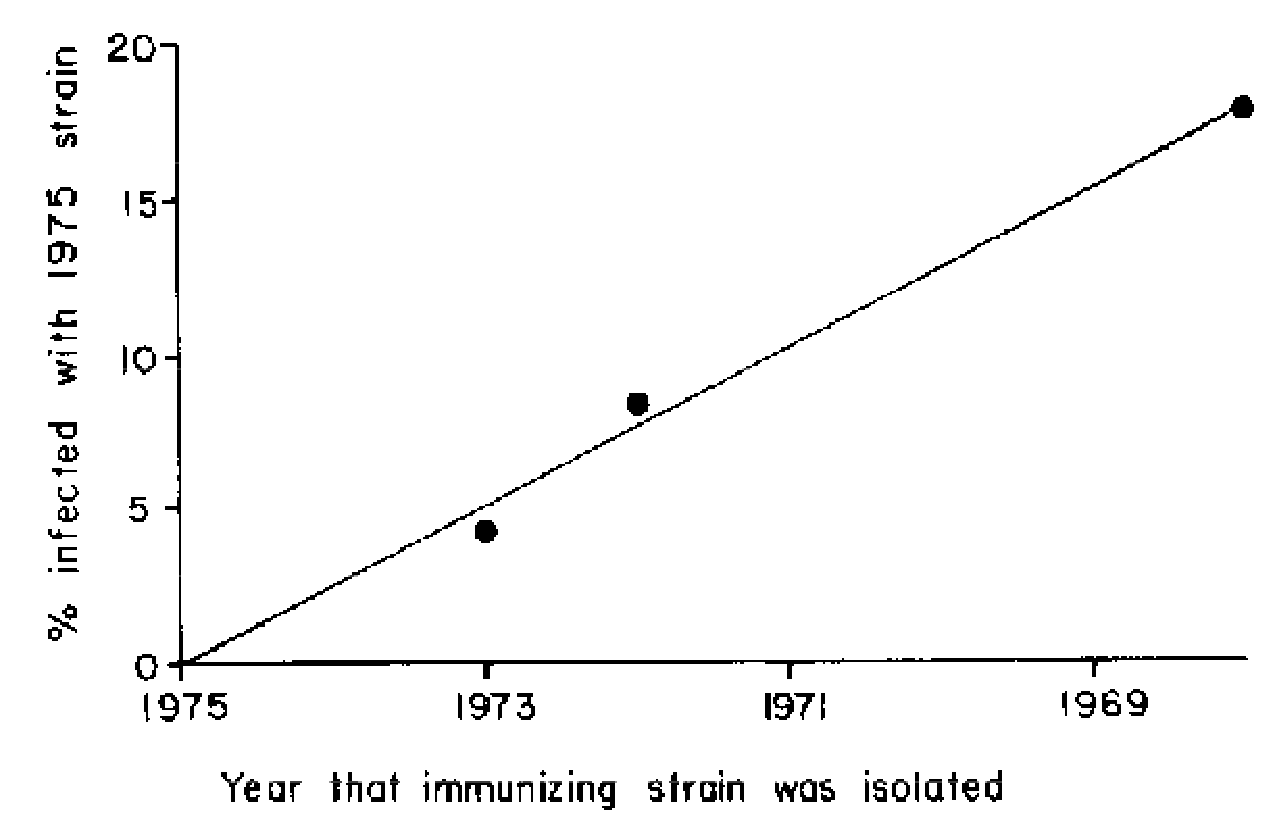
\includegraphics[width=0.5\linewidth]{graphs/intro/gill_murphy.eps}
  \end{center}
  \caption{Données de \citet{Gill1977} (reproduit d'aprés \citet{Pease1987})}
  \label{fig:intro:gill_murphy}
\end{figure}

L'expérience de \citet{Potter1977} permet de trancher entre ces
hypothèses. \citet{Potter1977} ont en effet immunisé des volontaires
avec différents vaccins dérivés de quatre souches de grippe A/H3N2
isolées en 1968, 1972, 1973 et 1974. Après 4 semaines, un temps
suffisamment court pour invalider l'hypothèse de la perte d'immunité,
ces volontaires ont été infectés par une souche virale de 1974. Les
résultats de cette expérience, présentés figure~\ref{fig:intro:potter}
montrent aussi une augmentation linéaire de la probabilité de
réinfection au fur et à mesure que le temps séparant les souches
immunisantes et le virus utilisé pour l'infection augmente. Cela
confirme l'hypothèse de l'augmentation du risque de réinfection du
fait de l'échappement des virus à l'immunité préexistante.

\begin{figure}[!htbp]
  \begin{center}
    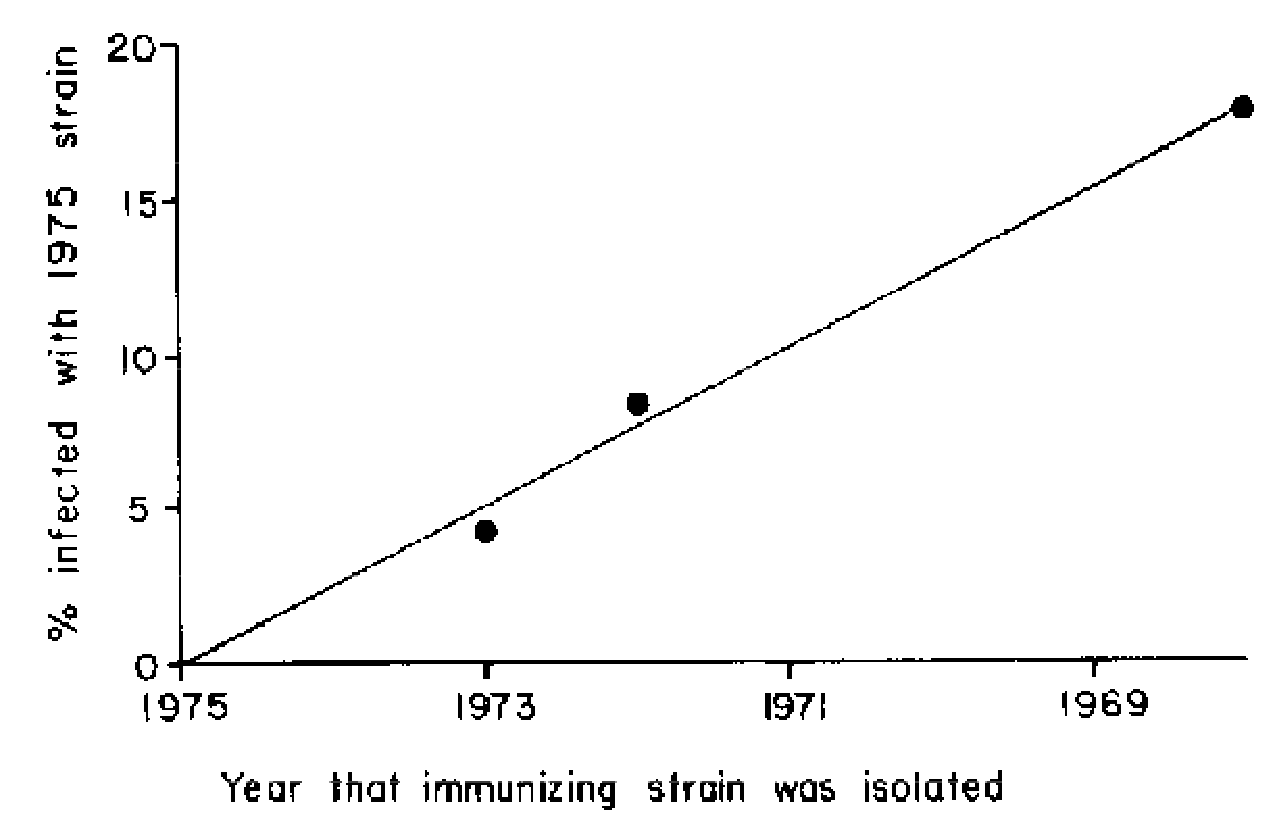
\includegraphics[width=0.5\linewidth]{graphs/intro/gill_murphy.eps}
  \end{center}
  \caption{Données de \citet{Potter1977} (reproduit d'aprés
    \citet{Pease1987})}
  \label{fig:intro:potter}
\end{figure}


Ce résultat permet à \citet{Pease1987} de proposer un nouveau modèle
pour les maladies récurrentes à évolution antigénique rapide.
Contrairement au paradigme classique des maladies infectieuses
infantiles où le renouveau des susceptibles se fait par les
naissances, dans le cas de la grippe ce renouveau de susceptibles se
fait par la perte d'immunité des hôtes du fait de l'évolution virale.
\citet{Pease1987} modélise alors l'évolution antigénique implicitement
par un changement de la susceptibilité des hôtes au cours du temps, en
accord avec les données disponibles à l'époque.

%\clearpage

\subsection{L'âge d'or de la génétique}

La révolution de la génétique des années 90 a permis l'acquisition
d'un nombre impressionnant de nouvelles données et une avancée majeure
dans la compréhension de l'évolution de la grippe A humaine. Les
années 90 ont donc vu les premières publications par \cite{Fitch1991}
et \citet{Fitch1997} de l'analyse phylogénétique des séquences du gène
HA1 (la région la plus immunogène de l'hemagglutinine).
\citet{Fitch1997} utilisent ainsi 254 séquences de HA1 obtenues de
1984 à 1996. Comme nous l'avons indiqué précédemment, cette étude a
révélé une diversité génétique relativement réduite à chaque instant
avec un arbre caractérisé par un tronc marqué comprenant de très
courtes branches. \citet{Fitch1997} ont ainsi montré que la durée
moyenne de survie des branches n'était que de 1.42 ans avec une durée
de 4.8 ans pour la branche la plus longue. Le nombre de substitutions
de nucléotides donnant lieu à des remplacements est 2.2 fois plus
élevé dans les branches que sur le tronc. Ce résultat peut s'expliquer
de différentes façons. On peut supposer que cet excès de mutations
dans les branches correspond à des mutations délétères (largement
majoritaires parmi les mutations) non encore purgées par la sélection
naturelle, et donc qui ne se retrouveront pas dans le tronc
ultérieurement. Cette hypothèse est intéressante, cependant en raison
des biais induits par le processus d'échantillonage et d'obtention des
séquences, elle ne peut être validée (nous verrons plus tard comment
les modèles multi-souches peuvent éclairer cette question). En effet
8\% des remplacements d'acides aminés observés sur HA1 peuvent être
attribués à des mutations liées à l'adaptation du virus aux oeufs
embryonnés utilisés pour les cultiver \citep{Bush2000}. Tout comme les
mutations délétères, les mutations produites par les oeufs ne se
retrouveront pas dans le tronc ultérieurement et peuvent donc ainsi
rendre compte de cette différence. Un second biais à même de rendre
compte de cette différence vient du fait que les données sont
fortement biaisées en faveur de variations antigéniques car
l'essentiel des séquences sont obtenues uniquement après un premier
tri visant à reconnaître les souches virales les plus divergentes d'un
point de vue antigénique dans le but de déterminer les futures
compositions vaccinales dans le cadre du programme de surveillance
globale de la grippe mis en place par l'OMS depuis 1952
\citep{Bush2000}. L'étude de \citet{Fitch1997} a aussi été le point de
départ d'une meilleure compréhension des processus sélectifs opérant
sur l'antigène principal de la grippe. La flexibilité de HA1 a été
mise en évidence en révélant que le nombre de substitutions de
nucléotides donnant lieu à des remplacement d'acides aminés était
distribué aléatoirement sur la position des codons (alors que
généralement on observe plus de substitutions conduisant à des
remplacements sur la première que sur la seconde position, les
substitutions étant plus conservatrices si elles ont lieu sur la
première position des codons). \citet{Fitch1997} et \citet{Bush1999}
ont aussi mis en évidence, en prenant garde de ne pas retenir de faux
positifs, 18 sites ou le ratio de substitutions non synonymes sur
synonymes était supérieur à 1, indiquant de la sélection positive.

\citet{Bush1999} ont cherché à comprendre dans quelle mesure les
codons sélectionnés positivement précédemment identifiés pouvaient
permettre de prédire l'évolution de la grippe A. Ces auteurs ont
montré que les lignées comportant le plus de mutations au niveau des
18 sites soumis à la sélection positive étaient pour 9 saisons sur 11
de 1986 à 1997 les lignées donnant naissance aux futures lignées
fructueuses engendrant le tronc de l'arbre. D'une manière remarquable,
si ces 18 codons sont associés à la région de reconnaissance des
anticorps, les codons de ces mêmes zones non soumis à la sélection
positive n'ont pas le même pouvoir prédictif, leur utilisation ne
permettant d'identifier les lignées fructueuses que dans 3 dans 11
saisons.
% predictabilité remise en question par la suite car les sites
% séléctioné changent !!!

L'accès à un nombre toujours grandissant de génomes complets
séquencés, accompagnés d'une augmentation conjointe de la puissance de
calcul nécessaire à leur analyse \citep{Holmes2007}, ont depuis permis
de nouvelles avancées dans ce domaine. Nous les détaillerons dans les
parties \ref{sec:intro:clusters}, \ref{sec:intro:sourcesink} et
\ref{sec:intro:debat} après avoir présenté les apports des modèles
mathématiques théoriques.


\subsection{Les modèles multi souches}

Du coté théorique, après les travaux de \citet{Pease1987}, de
nombreuses études ont cherché à modéliser explicitement les
différentes souches pour se rapprocher des analyses phylogénétiques.

L'approche la plus intuitive consiste peut-être à regrouper les hôtes
selon leurs histoires d'infections (approche $HB$ pour ``History
based'') comme introduit par \citet{Andreasen1997}. Ainsi, connaissant
l'histoire d'infection de chaque hôte, on peut établir des hypothèses
concernant l'effet du répertoire immunitaire acquis, face à une
infection par une nouvelle souche. Deux grandes catégories
d'hypothèses non mutuellement exclusives peuvent être faites. On peut
supposer:
\begin{itemize}
\item que l'immunité acquise suite aux infections précédentes confère
  une réduction de susceptibilité, limitant le risque de devenir
  infectieux ;
\item ou bien, que la protection partielle conférée par les infections
  précédentes se traduit par une moindre infectiosité suite à
  l'infection par la nouvelle souche (le risque d'infection étant le
  même que pour un hôte totalement naïf).
\end{itemize}

Il est alors naturel de supposer que la réduction de susceptibilité
($RS$) ou d'infectiosité ($RI$) est d'autant plus grande que les
souches nous ayant immunisé et allant nous infecter diffèrent
antigéniquement (immunité croisée). Lorsqu'un hôte immunisé par
plusieurs souches rencontre une souche n'appartenant pas à son
répertoire immunitaire, deux formulations sont principalement
utilisées pour décrire la protection partielle \citep{Gomes2002}:
\begin{itemize}
\item l'une suppose que l'immunité croisée agit de façon
  multiplicative, des anticorps de tout le répertoire immunitaire de
  l'hôte étant produits et leur action combinée étant supérieure à
  celle de chacun d'eux pris individuellement ;
\item et l'autre, que la protection partielle la plus forte détermine
  l'immunité croisée. Dans ce dernier cas, uniquement les anticorps du
  répertoire immunitaire de l'hôte les plus proches de la souche
  rencontrée sont produits.
\end{itemize}

Le principal obstacle à cette approche vient du fait de l'explosion du
nombre de variables d'états avec l'augmentation du nombre de souches.
Ainsi, pour une population comprenant $K$ souches, il y a $\sum_k
\binom{K}{k}=2^K$ histoires d'infections possibles. Comme le montre la
figure~\ref{fig:intro:multi}, passé $K=30$, ce nombre dépasse le
milliard. On ne peut donc pas espérer suivre la dynamique d'un grand
nombre de souches avec une telle approche, et, très rapidement, une
approche individu-centrée devient plus tractable.

\begin{figure}[!ht]
  \begin{center}
    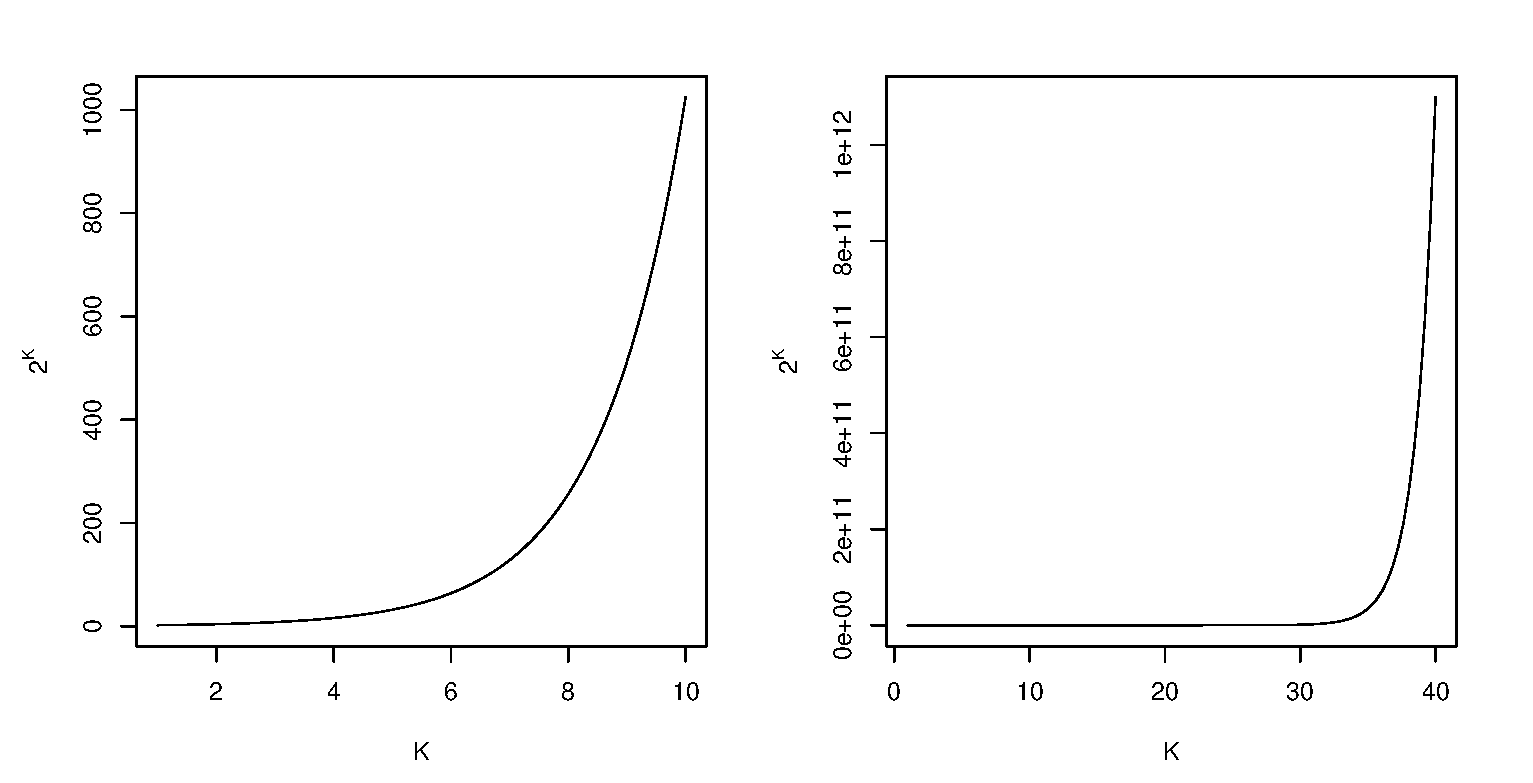
\includegraphics[width=0.8\linewidth]{graphs/R/multi.eps}
  \end{center}
  \caption{Augmentation du nombre de variables d'états en
    fonction du nombre de souches ($K$)}
  \label{fig:intro:multi}
\end{figure}

L'étude de la dynamique de système comprenant un petit nombre de
souches permet néanmoins de révéler des résultats intéressants comme
nous le montrerons par la suite (partie \ref{sec:intro:recyclage}).

Une autre approche des modèles multi-souches a été proposé par
\citet{Gog2002a}. Au lieu de suivre l'histoire infectieuse de la
population, ces auteurs ont proposé de suivre le statut immunologique
des hôtes en faisant l'hypothèse d'immunité croisée polarisée
(approche $SB$ pour ``status based''). Cette hypothèse suppose que le
statut immunologique est déterminé au moment de l'infection et résulte
immédiatement en l'acquisition d'une protection totale ou pas
(immunité polarisée) pour les souches antigéniquement voisines de la
souche infectante, selon des probabilités fonction de la distance
antigénique entre les souches. Considérons l'hypothèse $RS$ dans un
cas où il n'existe que 2 souches immunologiquement réactives (1 et 2)
pour mieux percevoir cette différence:
\begin{itemize}
\item Dans l'approche $HB$, l'infection par la souche 1 confère
  une protection partielle aux hôtes infectés ($R_1$). Cette
  protection ne s'applique que lors de la rencontre avec la souche
  2 antigéniquement proche et se matérialise par une probabilité
  réduite ($\sigma$) de devenir infecté par la souche 2. Si
  l'individu $R_1$ n'est pas infecté par la souche 2 lors de cette
  rencontre, il pourra l'être lors d'une rencontre ultérieure toujours
  avec la même probabilité réduite ($\sigma$).
\item Dans l'approche $SB$ le statut immunologique de notre hôte est
  déterminé au moment de l'infection par la souche 1. Selon une
  probabilité $\sigma'$, cet hôte acquiert une protection totale pour
  les souches 1 et 2 (devenant $R_{12}$).  Dans le cas
  complémentaire (probabilité $1-\sigma'$) il n'acquiert l'immunité
  que pour la souche 1 (devenant $R_1$) et reste donc totalement
  susceptible à la souche 2.
\end{itemize}

Les modèles $SB$ supposent aussi que l'immunité croisée agit de façon
multiplicative. En particulier, on suppose que les événements
d'acquisition d'immunité pour une souche $n$ lors d'une infection par
une souche $k$ (de probabilité $\sigma'_{kn}$) sont indépendants. On
peut ainsi calculer la probabilité $C(M,N,k)$ qu'un individu ayant un
statut immunologique $M$ acquiert un statut $N$, $M \subseteq N$,
suite à une infection par une souche $k$:

$C(M,N,k)$ =$
\begin{cases}
  \prod_{n \in N \setminus M} \sigma'_{kn} \prod_{n \notin N}
  (1-\sigma'_{kn}) & \text{si } k \notin M \text{ et } M \subset N \\
  0 & \text{sinon.}
\end{cases}$ 

où $N \setminus M$ dénote l'ensemble dont les éléments sont ceux de $N$ qui n'appartiennent pas à $M$. 


Une propriété remarquable de l'approche $SB$ a été mise en avant par
\citet{Gog2002}. Combiné à l'hypothèse $RI$ (et on autorisant la
coinfection), le formalisme basé sur le statut des hôtes permet de
réduire considérablement le nombre d'équations du système
multi-souches, en décrivant un système de $K$ souches avec exactement
$2K$ équations.

\citet{Gog2002} ont pu alors étudier comment différentes souches
immunologiquement réactives s'organisaient face à l'immunité
développée par une population d'hôtes. Ces auteurs ont considéré que
les souches évoluaient dans un espace unidimensionnel (une simple
ligne). Les souches pouvaient ainsi muter et donner naissance à des
souches filles voisines situées de part et d'autre de la souche
originelle. Un lien direct avec cet espace de souches permet de
modéliser l'immunité croisée, supposée décroître exponentiellement au
fur et à mesure que la distance entre les souches augmentent. Dans ce
contexte, \citet{Gog2002} révèlent que le système s'organise
différemment selon la durée de la période infectieuse des hôtes. Dans
le cas des maladies plutôt chroniques, différents clusters de souches
coexistent dans le temps, tandis que, pour des maladies à courte
période d'infection, des clusters de souches émergent et se remplacent
successivement au cours du temps. Ce dernier résultat n'est pas sans
rappeler les arbres phylogénétiques de HA1 précédemment décrits.
Ainsi, le système s'auto-organise, sous l'effet de l'immunité de la
population en groupe de souches aux propriétés antigéniques voisines.
\citet{Gog2002} montrent en particulier que leur modèle est en accord
avec l'hypothèse que les courtes branches latérales s'échappant du
tronc de l'arbre phylogénétique de HA1 pourraient être dues à des
souches ayant accumulé des mutations délétères, que nous avions énoncé
lors de la description des travaux de \citet{Fitch1997}. Pour ce
faire, ils utilisent un espace de souches bidimensionnel (un plan) où
la nouvelle dimension est associée à des mutations donnant lieu à des
virus moins transmissibles. Ils montrent alors que des virus
intrinsèquement moins transmissibles peuvent se maintenir un court
moment derrière les souches dominantes dont la progression engendre le
tronc d'un arbre. Le modèle de \citet{Gog2002} est donc remarquable
d'autant plus que l'aggrégation des souches en clusters antigéniques
sera montré empiriquement \citep{Plotkin2002, Smith2004}. Cependant
une des limitations de ces résultats est l'emploi d'un espace
antigénique de très faible dimension et donc très contraint.

\citet{Girvan2002} se sont intéressés à cette question en regardant
les conséquences de la dimensionalité de l'espace antigénique sur le
système multi-souches. Ces auteurs ont utilisé un modèle élégant
modélisant les séquences virales par des chaînes binaires. Dans ce
contexte, un espace antigénique de faible dimension peut être simulé
en supposant par exemple qu'à chaque mutation (représentée par le
changement d'un bit de 0 à 1) seul le bit le plus à gauche est muté.
Cela donne une évolution de la sorte:

\begin{verbatim}
00000000000000000
10000000000000000
11000000000000000
11100000000000000
\end{verbatim}

La distance antigénique est ensuite considérée en tenant compte du
nombre de différences entre les chaînes binaires présentes dans le
répertoire immunitaire de l'hôte et la souche infectante. Si la plus
petite de ces différences est supérieure à un seuil, l'hôte peut être
infecté, sinon, il est protégé.  \citet{Girvan2002} montrent que cet
espace antigénique contraint conduit à une diversité virale limitée et
produit des infections récurrentes en accord avec ce que l'on observe
pour la grippe.

La situation est par contre très différente lorsque l'on considère un
espace antigénique de grande dimension, obtenu par exemple en laissant
varier librement la position du bit mutant comme dans la séquence
ci-dessous:

\begin{verbatim}
00000000000000000
00000000010000000
00001000000000000
00000000010010000
\end{verbatim}

Dans ce cas, le nombre de souches ne cesse d'augmenter au cours du
temps, en désaccord avec les données phylogénétiques. Le modèle de
\citet{Girvan2002} incite donc à rechercher quels sont les facteurs
qui peuvent réduire le grand nombre de souches obtenu avec des modèles
considérant un espace antigénique réaliste de grande dimension.

\citet{Ferguson2003} s'attaquent à cette question dans un article
remarquable où ils considèrent un modèle individus centré, simulant
une population de 12 millions d'individus distribuée dans 20 patchs
géographiques où la transmission varie en opposition de phase dans
l'hemisphère Nord et Sud. Les souches sont caractérisées par
l'hémagglutinine et modélisées par 4 épitopes contenant chacun 3
codons. Ce système peut générer $4. 10^{15}$ souches. L'immunité
croisée varie en fonction d'une distance antigénique $d$ définie en
fonction du nombre de codons de la souche infectieuse n'ayant pas
d'acides aminés en commun avec ceux contenus dans le répertoire
immunitaire de l'hôte. \citet{Ferguson2003} suppose que l'immunité
croisée plafonne à une valeur élevée tant que $d$ est inférieur à 2
acides aminés puis qu'elle décroît linéairement jusqu'à une valeur
minimale.

Ces auteurs montrent d'abord que comme pour le modèle de
\citet{Girvan2002}, le système précédemment décrit conduit à une
explosion de la diversité de souches et une prévalence excessive. Ce
résultat est en particulier robuste à l'inclusion de contraintes
fonctionnelles. Cette explosion de diversité virale se comprend assez
bien étant donné que l'immunité croisée décroît avec la distance
antigénique. Ainsi, lorsque la diversité antigénique augmente, la
prévalence augmente aussi et cela renforce la production d'autres
variants. \citet{Ferguson2003} postulent alors l'existence d'un
processus de densité dépendance agissant à l'échelle de temps de
l'apparition des souches pour expliquer la réduction de la diversité
virale. Ces auteurs suggèrent que ce processus pourrait être le fait
d'une période temporaire de courte durée d'immunité totale (protégeant
contre toutes les souches et tous les sous-types de grippe) due à
l'action des lymphocyte T cytotoxique (CD8 +T) dirigée contre les
protéines internes du virus fortement conservées. L'importance de
cette composante de la réponse immunitaire avait été soulignée par
ailleurs par \citet{Webster1992} comme un des facteurs pouvant
expliquer le remplacement des sous-types grippaux lors des précédentes
pandémies dans un contexte où l'immunité croisée entre les sous-types
est présumée être faible. Les lymphocytes CD8 +T sont considérés
importants pour la guérison d'une infection grippale mais ne sont
généralement pas suffisants pour protéger contre les réinfections
ultérieures en l'absence d'anticorps. En effet, leur quantité diminue
trop rapidement après la première infection pour rester effective et
le temps nécessaire à leur rappel est trop élevé pour empêcher
l'établissement d'un nouveau virus \citep{Grebe2008}.

\citet{Ferguson2003} montrent que l'inclusion de cette période
temporaire d'immunité totale (les auteurs la prennent égale à 6 mois)
suffit à réduire la diversité virale, et permet d'obtenir des
phylogénies identiques à celles obtenues pour HA de H3N2. Ils montrent
en outre que la réduction du taux de mutation et de l'intensité de
l'immunité croisée permet d'obtenir des phylogénies avec plusieurs
lignées co-circulantes, comme c'est le cas pour la grippe B et dans
une moindre mesure H1N1, la valeur de $R_0$ n'ayant que peu
d'influence. Les auteurs confirment les prédictions de
\citet{Webster1992} et montrent que la période d'immunité croisée est
cruciale pour obtenir des remplacements de sous-types lors des
pandémies. Ils parviennent aussi à reproduire le cas de la
réintroduction de H1N1 en 1977 qui mène à la coexistence avec H3N2.

Le modèle de \citet{Ferguson2003} est séduisant sous bien des aspects,
cependant sa complexité rend son étude difficile. En particulier, il
est difficile de bien caractériser les chaînes causales menant aux
dynamiques observées. \citet{Tria2005} ont donc proposé de regarder
quels sont les facteurs minimaux pouvant expliquer les résultats de
\citet{Ferguson2003}. Pour ce faire ils ont considéré un modèle proche
de celui de \citet{Girvan2002} et négligé tous les processus spatiaux
inclus dans le modèle de \citet{Ferguson2003}. \citet{Tria2005}
partent d'un modèle de base ne comportant que de l'immunité croisée et
montrent que la présence additionnelle de la seule période d'immunité
temporaire totale ne suffit pas à réduire la diversité virale. Pour
retrouver un nombre de souches réduit, cette période de protection
totale doit être accompagnée d'une forme d'hétérogénéité.
\citet{Tria2005} l'incluent en supposant que les mutants ont des taux
de transmission variables tirés dans une loi Gamma. Ils supposent que
cette hétérogénéité est aussi présente dans le modèle de
\citet{Ferguson2003} par l'intermédiaire de la dynamique spatiale.

Cependant, une différence importante existe dans la façon dont
\citet{Ferguson2003} et \citet{Tria2005} ont modélisé la période
temporaire d'immunité croisée. \citet{Tria2005} ont simplement supposé
qu'une fois guéris, les hôtes restaient un temps défini
``invincible'', tandis que \citet{Ferguson2003} ont considéré en plus
que toutes les expositions ne donnant pas lieu à une infection étaient
suivies d'un ``boosting'' de la période d'invincibilité (alors étendue
de sa durée moyenne) sans mise à jour du répertoire immunitaire. Les
auteurs justifient ce processus par l'existence du péché antigénique
originel (\citet{Francis1953}, \citet{St1966}, \citet{St1966a} ou
\citet{Kim2009} pour une synthèse récente) qui établit que lors
d'infections séquentielles, la réponse immunitaire cible
préférentiellement les antigènes de la souche rencontrés initialement
plutôt que les antigènes mutés de nouvelles souches antigeniquement
proches, permettant à ces nouveaux virus d'échapper en grande partie à
la réponse immunitaire.  Notons que le péché antigénique originel
justifie le fait de ne pas mettre à jour le répertoire immunitaire des
expositions à des souches antigéniquement proche ne donnant pas lieu à
des infections mais il ne justifie pas nécessairement de ``booster''
la période d'invincibilité des hôtes rencontrant des souches pour
lesquelles ils sont déjà immunisés et ne redeviennent pas infectieux.
Ce ``boosting'' additionnel est reporté comme une contrainte densité
dépendante importante réduisant la diversité virale, l'incidence et
les taux de fixation dans les annexes de leur papier et nous supposons
que cette différence majeure peut être à l'origine des résultats
rapportés par \citet{Tria2005}.

\citet{Minayev2008, Minayev2009} ont proposé un modèle analytique
cherchant à se rapprocher du modèle de \citet{Ferguson2003}. Ils ont
donc mis de côté l'approche $SB$ impliquant une immunité croisée
multiplicative et ont privilégié le formalisme $HB$.  Leur modèle est
basé sur celui de \citet{Gupta1998} qui ont montré qu'en décrivant les
souches par un système génétique de $L$ loci comprenant $A$ allèles,
on pouvait obtenir un système dont le nombre d'équations augmente
linéairement avec le nombre de souches (donné par $A^L$) à condition:
\begin{itemize}
\item d'utiliser des variables d'états se recoupant,
\item de permettre la coinfection,
\item et de considérer une forme spéciale de l'hypothèse de
réduction d'infectiosité décrite ci-dessous. 
\end{itemize}
Dans le modèle de \citet{Gupta1998}, les hôtes partiellement protégés
sont tous totalement susceptibles à une souche immunologiquement
réactive, mais suite à l'infection, seulement une partie des hôtes
infectés deviennent infectieux, la partie complémentaire acquérant une
immunité pour la souche rencontrée sans devenir infectieux.  Dans sa
version originale, ce modèle ne prévoyait qu'un seul niveau d'immunité
croisée selon que les souches aient un allèle en commun ou pas.
\citet{Minayev2008} ont généralisé ce modèle pour prendre en compte
différents niveaux d'immunité croisée (en supposant que la protection
croisée soit définie par le nombre d'alléles en commun des souches)
tout en gardant un nombre d'équations augmentant linéairement avec le
nombre de souches. Ce modèle, sans doute le plus tractable dans les
approches $HB$ comporte au final ``seulement'' $A^L(L+1)$ équations.

\citet{Minayev2008, Minayev2009} confirment alors l'explosion de la
diversité virale en l'absence de période d'immunité totale temporaire.
Ces auteurs veulent ensuite étudier l'effet de la période
d'invincibilité (en l'introduisant tout comme \citet{Ferguson2003} et
donc en considérant un ``boosting'' de la période d'invincibilité sans
mise à jour du répertoire immunitaire suite aux expositions ne donnant
pas lieu à des infections). Leurs résultats sont dans ce cas à prendre
avec précaution car les équations introduisant la période
d'invincibilité temporaire sont inconsistantes.  Brièvement,
l'équation (4.2) de \citet{Minayev2008} (respectivement équation (2.6)
dans \citep{Minayev2009}) stipule que les infections peuvent provenir
d'une souche déjà présente dans le répertoire immunitaire et que dans
ce cas, les hôtes ne deviennent pas infectieux mais développent une
invincibilité de 6 mois.  Cependant, les auteurs précisent aussi que
l'équation (2.1) des 2 papiers reste identique ce qui est en
contradiction avec l'équation (4.2) (respectivement (2.6)) étant donné
le fait que l'équation (2.1) implique que les hôtes ne peuvent pas
être infectés ou développer une immunité totale temporaire s'ils sont
exposés à des souches déjà présentes dans leur répertoire
immunitaire. Il faudrait donc revisiter les parties de ces papiers
impliquant la période d'immunité totale temporaire avant d'en tirer
des conclusions.

%\clearpage

\subsection{Les clusters antigéniques}
\label{sec:intro:clusters}

Du coté des donnés, \citet{Plotkin2002} ont utilisé une approche
complémentaire à la reconstruction phylogénétique en regardant s'il
existait une unité naturelle d'agrégation des différentes souches.
\citet{Plotkin2002} ont ainsi montré que l'on pouvait regrouper
différentes souches en clusters en considérant par exemple comme
critère de regroupement le nombre d'acides aminés différents (distance
de Hamming). Les clusters, définis à partir de 560 séquences du gène
codant pour la région HA1 de l'HA de H3N2 échantillonné entre 1968 et
2000, apparaissent se succéder au cour du temps et se remplacent tous
les 2-5 ans, rappelant les résultats obtenus par \citet{Gog2002}. Ces
clusters, définis uniquement à partir de la séquence d'acides aminés,
se trouvent être en plus de bons prédicteurs de la propriété
antigénique des virus sous-jacents. En particulier, en utilisant la
souche la plus récente du cluster dominant d'une saison de grippe
donnée, \citet{Plotkin2002} obtiennent des recommandations vaccinales
identiques à celles de l'OMS, basées sur la caractérisation des
propriétés antigéniques des souches, pour 9 des 16 saisons
considérées. Ces auteurs révèlent des relations intéressantes entre la
variation des acides aminés au cours du temps pour les 5 épitopes
majeurs de HA1 aussi bien au sein qu'entre les clusters. Il apparaît
en particulier, que chaque changement de cluster est principalement le
résultat d'une forte variation au sein d'un épitope, lui-même
différent de l'épitope le plus variable lors du précédent changement
de cluster. Enfin, une forte corrélation est reportée entre la
variation d'acides aminés intra cluster et la distance selon la
métrique de Haming entre les différents clusters. Tout se passe donc
comme si les changements entre clusters n'étaient possibles que
lorsque la sélection naturelle a suffisamment de variabilité au sein
d'un cluster pour s'exprimer.

La mise en avant des clusters comme unité de base sur laquelle fonder
un raisonnement évolutif par \citet{Plotkin2002} a été largement
confirmée et précisée par les travaux de \citet{Smith2004}.
\citet{Smith2004} se sont intéressés au lien qu'il y avait entre
génotype et phénotype (en particulier la propriété antigénique).
L'inférence des propriétés antigéniques des HA des différentes souches
est réalisée par le test d'inhibition de l'hemagglutination (HI)
\citep{Miller1944}. Ce test repose sur la capacité de l'HA des virus
grippaux à agglutiner des globules rouges et à la capacité de sérum
animaux produits par réaction aux différents virus grippaux à inhiber
cette agglutination (plus ou moins bien en fonction de la distance
antigénique séparant les virus). Cette technique est utilisée de
manière standard par l'OMS pour établir les compositions vaccinales.
En particulier, il est considéré qu'une dilution de facteur 4 du sérum
lors du test HI impose de mettre à jour le vaccin. Utilisant une
approche multivariée, \citet{Smith2004} ont pu révéler les relations
antigéniques de 273 isolats (dont 94 proviennent de Hollande, les
autres du reste du monde) prélevés entre 1968 et 2003 soumis à des
test HI croisés. Ces auteurs montrent ainsi que s'il existe une
correspondance remarquable entre l'évolution génétique et antigénique
des virus, des différences significatives existent. Si l'évolution
génétique du virus est largement graduelle, l'évolution antigénique
est elle ponctuée. Les différentes souches s'organisent en clusters
présentant des propriétés antigéniques semblables, et les clusters
restent dominant entre 1 et 8 saisons avec une moyenne 3.3 ans ($\pm
1.9$) avant d'être remplacés. En particulier, l'évolution antigénique
s'opère principalement dans un espace à 2 dimensions dans lequel les
clusters s'organisent chronologiquement selon un axe majoritaire
accompagné de variations ``en zigzag'' dans l'autre dimension
(figure~\ref{fig:intro:smith}).  Les transitions de clusters sont le
fait d'un nombre variable de changements d'acides aminés. Le
changement d'un seul acide aminé peut suffire à précipiter un
changement de cluster. C'est par exemple le cas de la mutation N145K
liée à la transition du cluster SI87 à BE89 et BE92 à WU95. Les
changements d'acides aminés corrélés aux changements de clusters
antigéniques correspondent à l'étude des codons sous sélection
positive par \citet{Bush1999} uniquement pour la période 1985-1997
correspondant aux séquences de cette dernière étude.  L'absence de
correspondance pour les autres périodes temporelles va de pair avec
l'hypothèse d'un changement des sites sélectionnés au cours du temps
déja révélé par \citet{Plotkin2002} et posant des limites à la
possibilité de prédire l'évolution de HA1 comme l'avait laissé
entrevoir l'étude de \citet{Bush1999}.

\begin{figure}[!htbp]
  \begin{center}
    \includegraphics[width=0.5\linewidth]{graphs/intro/smith.eps}
  \end{center}
  \caption{Cartographie antigénique des virus A/H3N2 isolé de 1968 à
    2003. (reproduit d'après \citet{Smith2004}).}
  \label{fig:intro:smith}
\end{figure}


\citet{Blackburne2008} se sont intéressés à cette question en
comparant différents modèles d'évolution moléculaire d'une complexité
croissante pouvant être sélectionnés par AIC ou ratio de vraisemblance.
En utilisant les même données que \citet{Smith2004} (254 séquences
isolées de 1968 à 2003) ces auteurs montrent que le modèle le plus
adapté pour rendre compte des données comporte un ensemble de matrices
de substitutions différentes pour différentes régions de la protéine
et où le taux de substitution peut changer au cours du temps,
correspondant à un changement de pressions de sélection.
\citet{Blackburne2008} valident ainsi l'hypothèse que les sites de HA1
soumis à la sélection positive varient au cours du temps, rendant la
distinction entre site antigénique et non antigénique plus subtile et
labile que précédemment considérée. En particulier, ces auteurs
montrent que beaucoup de changements de pressions de sélection ont
lieu au niveau de sites non directement associés au changement
d'acides aminés menant à des transitions de clusters antigéniques. Ces
mutations peuvent être impliquées dans le maintien de la
fonctionnalité de HA (potentiellement mise à mal par les autres
changements ayant conduit à des modifications des propriétés
antigéniques), ou bien encore, peuvent assurer la stabilité
thermodynamique de la macromolécule.

Du coté théorique, \citet{Koelle2006} ont montré que le caractère
ponctué de l'évolution antigénique de HA de la grippe A/H3N2 se
révélait être primordiale dans la détermination de la phylodynamique
du virus.  Influencés par le papier de \citet{Smith2004},
\citet{Koelle2006} se sont en particulier intéressé au lien qu'il
existe entre génotype et phénotype de HA. Là où les approches
précédentes avaient considéré un lien linéaire entre séquence
génétique et propriété antigénique, \citet{Koelle2006} ont modélisé ce
lien explicitement par un modèle de réseau neutre pour protéine
appliqué à HA. Schématiquement ce modèle suppose l'existence de
périodes où la structure de l'antigène varie peu, dû au fait que les
mutations sont principalement des mutations neutres ou quasi neutres
(peu d'influence sur la stucture tridimensionnelle de la protéine),
tandis que ponctuellement, de rares mutations peuvent précipiter un
changement de structure tridimensionnelle de l'antigène (et donc
grandement changer les propriétés antigéniques). Ce modèle prend en
compte les interactions complexes entre les différents acides aminés
des épitopes et accorde une importance au contexte dans lequel chaque
mutation apparaît. La considération d'un lien non linéaire et dégénéré
entre génotype et phénotype permet une interprétation aisée des
clusters antigéniques mis en évidence par \citet{Smith2004}.  En
particulier, il permet de rendre compte du fait que certaines
transitions de clusters sont le fait d'une seule mutation
(apparaissant dans un contexte particulier) tandis que certains
clusters gardent une même propriété antigénique tout en arborant une
grande variété de souches (par exemple 2 souches du cluster HK68
diffèrent de 19 acides aminés). Le modèle de réseau neutre pour HA est
aussi consistant avec la mise en évidence par \citet{Plotkin2002} d'un
lien entre l'accumulation de diversité d'acides aminés au sein d'un
cluster et le changement de cluster.

Au niveau épidémiologique, \citet{Koelle2006} modélise alors la
dynamique des clusters antigéniques du sous-type H3N2 en se focalisant
sur le niveau du phénotype. Par souci de simplicité,
\citet{Koelle2006} utilisent le modèle de \citet{Gog2002} (approche
$SB$ et hypothèse $RI$) et rajoutent un terme de forçage saisonnier
pour s'intéresser aux régions tempérées d'où proviennent l'essentiel
des données. Les auteurs sont obligés de prendre en compte une
structure spatiale implicite faisant intervenir une forte immigration
pour compenser les extinctions observées pendant la période
inter-épidémique. Partant de cette base, \citet{Koelle2006} montrent
que leur modèle permet d'obtenir des dynamiques très proches de celles
observées dans les zones tempérées. En particulier, le modèle prédit
une augmentation de la diversité virale jusqu'à ce qu'un nouveau
cluster antigénique apparaisse et que, du fait de son échappement à
l'immunité de la population, il soit suffisamment avantagé pour
remplacer le cluster précédent dans un balayage sélectif. Ainsi, la
diversité virale reste limitée dans le temps, et le modèle reproduit
la succession de clusters antigéniques observés. Au niveau
épidémiologique, les transitions de cluster s'accompagnent
généralement d'une épidémie plus marquée, souvent suivie d'une période
réfractaire (faible épidémie de H3N2) la saison suivante.
\citet{Koelle2006} remarquent que cette tendance est présente dans les
données des USA avec une période réfractaire observée pour 6 des 7
changements de clusters postérieurs à HK68. D'une manière remarquable,
dans 6 de ces 7 périodes réfractaires potentielles, H1N1 ou la grippe
B domine.

Le modèle de \citet{Koelle2006} illustre donc que la prise en compte
de l'évolution ponctuée de HA et donc l'échappement ponctué à
l'immunité de la population par la grippe suffit à rendre compte des
principales caractéristiques de H3N2. En particulier, la présence
d'une période d'immunité totale temporaire n'est pas nécessaire pour
expliquer la diversité génétique réduite observée dans les
phylogénies.  Par ailleurs, \citet{Koelle2006} rapportent que des
valeurs de $R_0$ plus faibles que celles utilisées pour leurs
simulations de H3N2 ($R_0 =5$) induisent des dynamiques durant
lesquelles des clusters antigéniques coexistent et les phylogénies
présentent plus de branchements, en accord avec ce que l'on observe
pour H1N1 et la grippe B.


Indépendemment des réseaux neutres, le modèle de \citet{Koelle2006}
met en évidence l'importance potentielle des balayages sélectifs et
des dynamiques transitoires comme éléments clefs pour comprendre la
phylodynamique de la grippe. Cette idée maîtresse peut donc aussi
s'appliquer lors des réassortiments intra-sous-type pouvant être
considérés dans certains cas à l'échelle du phénotype comme de rares
``mutations'' ayant de grands effets antigéniques. Les analyses de
génomes entiers, font en effet de plus en plus apparaître les
réassortiments intra-sous-type comme des évènements évolutifs
important pour la grippe \citep{Holmes2005, Nelson2007}. Par exemple,
dans une étude phylogénétique de 156 génomes complets de H3N2
collectés dans l'état de New York entre 1999 et 2004,
\citet{Holmes2005} ont montré que l'origine du cluster antgénique FU02
était dû à un réassortiment intra-sous-type entre différentes lignées
co-circulant de H3N2.  Cependant les exemples les plus marquants sont
peut-être ceux concernant H1N1. Au niveau épidémiologique, les
épidémies de 1947 et 1951 sont particulièrement marquantes. En 1947,
le vaccin alors efficace les années précédentes est un échec total et
les souches grippales apparaissent tellement différentes de celles des
années antérieures que la littérature de l'époque parle d'une nouvelle
famille de virus (A', par opposition à A les années précédentes).
\citet{Kilbourne2002} reviennent sur cette épidémie et montrent que
les HA des souches des familles A et A' n'ont que 5\% de réactivité
antigénique. Pour l'épidémie de 1951, \citet{Viboud2006b} montrent que
son impact en termes de mortalité et sa transmissibilité sont plus
élevés que lors des pandémies de 1957 et 1968 au Royaume unis et au
Canada. Une partie des causes de ces épidémies particulières ont été
révélées par l'analyse de \citet{Nelson2008}. Les auteurs ont analysé
71 génomes complets de H1N1 échantillonnés entre 1918 et 2006. Ils
montrent que l'épidémie de 1947 est liée à un réassortiment intra
sous-types permettant au virus prédominant de 1943 à 1945 d'acquérir
de nouveaux fragments d'ARN codant pour PB2, PA, HA, NP et NS
provenant vraisemblablement d'une lignée de H1N1 minoritaires et non
mise en évidence lors de la surveillance de l'époque. Le changement de
HA explique ainsi la forte divergence antigénique de la souche de
1947. Pour 1951, la même étude révèle que cette épidémie est
probablement liée à un réassortiment où les souches prédominantes
auraient gardé le même fragment d'ARN pour HA, mais acquis deux
nouveaux gènes codant pour les polymerases PB1 et PA.

Ces résultats montrent l'importance des réassortiments intra-sous-type
mais permettent aussi de tempérer un peu la vision simplifiée offerte
par la théorie de l'échappement ponctué à l'immunité. En effet, les
épidémies de 1947 et 1951 nous rappellent que la variation de HA n'est
pas toujours le déterminant majeur gouvernant la taille des épidémies.
L'épidémie de 1951, où à priori les deux antigènes principaux (HA et
NA) n'ont pas changé, a en effet été plus sévère que celle de 1947 où
un HA radicalement différent des précédents a émergé. Les interactions
entre les différents fragments du génome sont donc essentiels à
prendre en considération si l'on veut bien appréhender les
conséquences de l'évolution virale sur les dynamiques épidémiologiques
et la rétroaction qui s'en suit. Nous rediscuterons de ce point de
manière détaillée par la suite (partie \ref{sec:intro:sourcesink}).

Pour conclure cette section, il est intéressant de constater que le
changement de paradigme concernant l'évolution antigénique de la
grippe A permet de concilier deux hypothèses débattues dans les années
1950 et 1960, illustrées par les figures~\ref{fig:intro:francis1}
et~\ref{fig:intro:francis2}.

\begin{figure}[!htbp]
  \begin{center}
    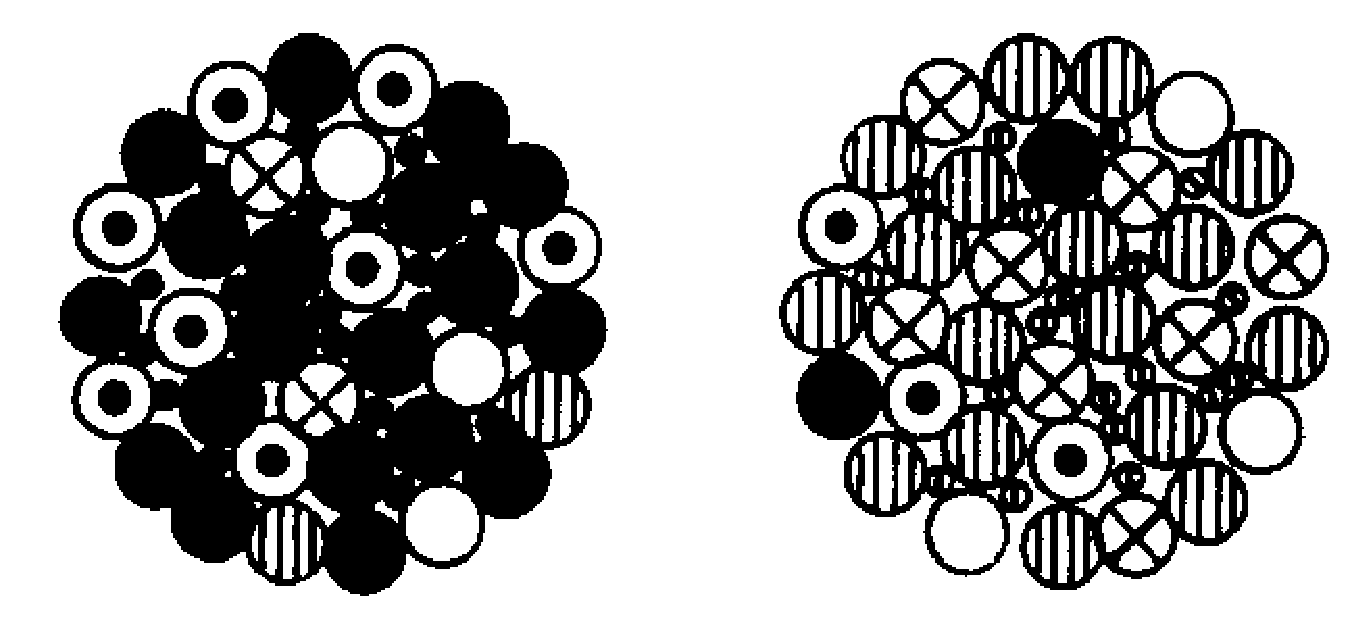
\includegraphics[width=0.5\linewidth]{graphs/intro/francis1.eps}
  \end{center}
  \caption{Illustration de l'hypothèse selon laquelle les variations
    antigéniques de la grippes sont le fait de rearangements d'un
    nombre fini d'antigènes (reproduit d'après \citet{Francis1960}).}
  \label{fig:intro:francis1}
\end{figure}

\begin{figure}[!htbp]
  \begin{center}
    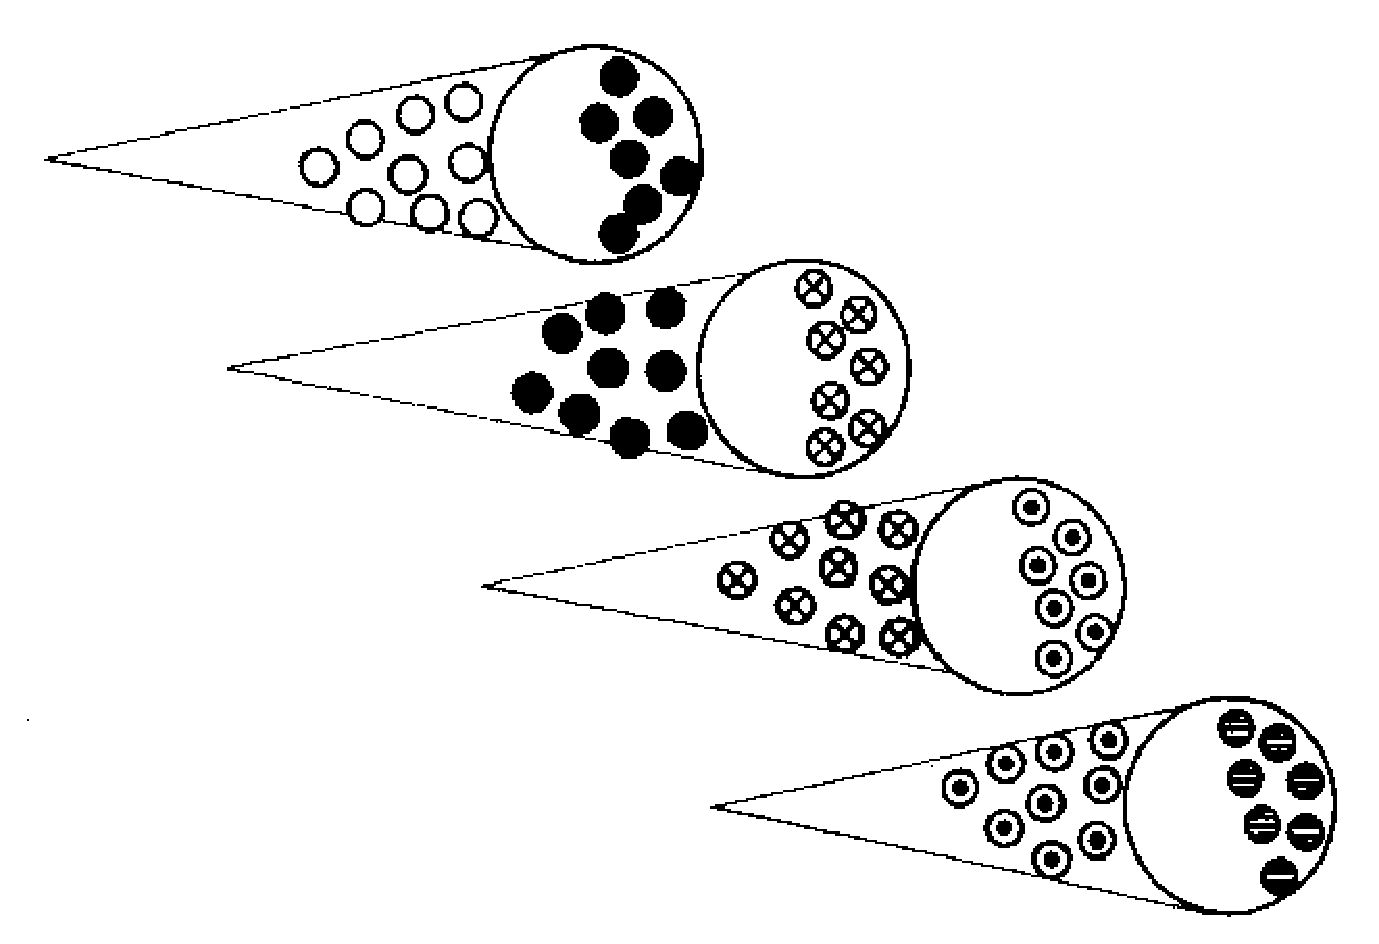
\includegraphics[width=0.5\linewidth]{graphs/intro/francis2.eps}
  \end{center}
  \caption{Illustration de l'hypothèse de la perte et gain d'antigènes
    pour les variants successifs de grippes (reproduit d'après
    \citet{Francis1960}).}
  \label{fig:intro:francis2}
\end{figure}

Les interrogations portaient sur la nature des changement antigéniques
des virus avec en confrontation, une vision selon laquelle ces
changements étaient le fait de ré-arrangement de différent antigènes
présents en un nombre fini, face à une vision où les changements
antigéniques résultaient du remplacement de différents antigènes au
cour du temps \citep{Francis1960}.

L'étude de \citet{Jensen1957} entre autre, avait permis d'opter pour
la première de ces hypothèses (figure~\ref{fig:intro:francis1}).  Les
auteurs ont caractérisé les propriétés antigéniques des variants de
H1N1 des familles A de 1933 à 1944 et A' de 1946 à 1955.  Pour ce
faire, ils ont établi un indice de réaction pour chaque souche défini
comme le nombre de souches avec lesquelles la souche étudiée interagit
fortement. Ainsi, une souche antigéniquement identique à toutes les
souches d'une série de 28 aura un indice de 28. Avec cette mesure, si
de nouveaux antigènes ne cessent d'apparaître au cours du temps, on
s'attend à observer une évolution croissante des indices. Si par
contre le nombre d'antigènes diminue, les indices devraient décroître
au cours du temps. Enfin, dans le cas où les antigènes se remplacent,
ont devrait avoir une courbe en cloche avec un maximum à mi-temps pour
les 2 familles. \citet{Jensen1957} révèlent que la distribution des
indices au sein de chaque famille (A et A') ne suit aucune de ces
évolutions. Les indices varient bien, indiquant une variabilité
antigénique mais sans tendance particulière au cours du temps.

Les résultats de \citet{Koelle2006} et, \citet{Blackburne2008}
permettent d'unifier ces deux hypothèses en attribuant la première à
des changements antigéniques intra-cluster et la seconde aux
transitions entre les clusters suivies de balayages sélectifs et de
changements de sites soumis à la sélection positive.

%\clearpage

\subsection{Une évolution antigénique graduelle ou ponctuée ?}
\label{sec:intro:debat}

\citet{Wolf2006} ont fourni une confirmation du changement de
perspective majeure dans l'appréhension de la dérive antigénique de la
grippe.  Ces auteurs ont utilisé plus de 1000 génomes complets
séquencés obtenus entre 1995 et 2005 pour les grippes A/H3N2 et
A/H1N1. Contrairement aux analyses précédentes, ces prélèvements ne
sont pas biaisés en faveur de la variation antigénique offrant la
garantie d'un meilleur reflet des différences de fitness entre les
lignées.  En accord avec les études antérieures, \citet{Wolf2006} ont
mis en évidence de la sélection positive (avec un ratio de
substitutions non synonymes sur synonymes supérieur à 1) pour les
sites situés au niveau du tronc de l'arbre appartenant à la région des
épitopes de HA.  Aucune trace de sélection positive n'a été détectée
en dehors de ces régions.  Le résultat n'apparaît cependant pas
statistiquement significatif, très probablement en raison du nombre
trop restreint de mutations sur le tronc de l'arbre pour avoir une
puissance suffisante. \citet{Wolf2006} ont ensuite cherché des
signatures de la sélection positive en considérant les temps
d'extinction des différentes lignées, définies arbitrairement à chaque
point de branchement de l'arbre phylogénétique pour la région de
HA. Les auteurs ont trouvé que la distribution des temps d'extinction
était bimodale avec des lignées caractérisées par de courts temps
d'extinction (inférieur à 6 mois), et d'autres, marquées par un temps
d'extinction beaucoup plus lent (supérieur à 6 mois). Dans ce
contexte, des temps d'extinctions courts sont à relier à un
remplacement rapide des nouvelles lignées, ce qui va dans le sens d'un
avantage sélectif pour les lignées capables de remplacer rapidement
leur prédécesseur. Cette idée est renforcée par la présence d'un excès
significatif de substitutions non synonymes pour les sites des
épitopes situés dans les régions du tronc caractérisées par des temps
d'extinctions rapides. Ces résultats amènent \citet{Wolf2006} à
conclure que l'essentiel de la sélection positive à lieu pendant de
courtes périodes (matérialisées par les régions du tronc associées à
des remplacements de lignées rapides) entre lesquelles se déroulent
des périodes plus longues de stase évolutive (matérialisées par les
régions du tronc ou les temps d'extinctions des lignées sont
lents). Par ailleurs, la présence de nombreuses mutations identiques
ayant lieu dans des lignées multiples majoritairement pendant ces
``bursts'' de sélection positive laisse à penser que le nombre de
trajectoires évolutives possible est limité.

\citet{Wolf2006} se sont aussi intéressés aux conséquences
épidémiologiques de leurs résultats. En particulier, n'ayant pas
détecté de traces de séléction positive pour HA de H1N1, ces auteurs
ont proposé que la dominance de H1N1 pendant certaines saisons de
grippes pouvait être due au fait d'une diminution de fitness relative
de H3N2, résultant d'une déplétion de la population d'hôtes
susceptibles à H3N2 non renouvelée durant les intervalles de stase
évolutive de ce sous-types. \citet{Wolf2006} rapportent ainsi qu'aux
Etats-Unis, les saisons de H3N2 précédent H1N1 sont caractérisées par
une diffusion significativement plus lente et un impact tendant a être
plus faible en terme de mortalité. L'accord de ces résultats avec
l'idée de période réfractaire mise en avant par \citet{Koelle2006}
n'est pas claire. En effet, d'après \citet{Koelle2006}, les périodes
réfractaires sont généralement précédées d'une saison de H3N2 plus
marquée, associée à un changement de cluster antigénique.

\citet{Shih2007} ont tempéré le paradigme naissant de l'évolution
antigénique ponctuée de HA pour H3N2. Ces auteurs ont cherché à mieux
caractériser le nombre de sites soumis à la séléction positive en
utilisant 2248 séquences de la région HA1 collecté entre 1968 and
2005.  \citet{Shih2007} ont analysé l'évolution de la fréquence des
acides aminés au cours du temps. L'étude des temps de fixation (connus
sous un modèle neutre) leur permet alors de détecter la présence de
sélection positive. Cette approche s'est révélée être relativement
puissante, leur permettant ainsi de retrouver la plupart des sites mis
en avant dans les études antérieures (ils retrouvent par exemple les
11 sites de HA1 où \citet{Wolf2006} ont détecté des remplacements
parallèles). Forts de cette analyse, \citet{Shih2007} révèlent qu'il
existe des mutations sélectionnées positivement d'une manière continue
dans le temps et non pas uniquement pendant de courtes périodes. Par
ailleurs, ils révèlent l'existence de nombreuses fixations simultanées
de différents acides aminés résultant vraisemblablement d'effet
cumulatif (épistasie). Ces résultats suggèrent donc que les
changements antigéniques pourraient être moins ponctués que ce qui
avait été proposé. En particulier \citet{Shih2007} rappellent que la
variation antigénique au sein des clusters identifiés par
\citet{Smith2004} est toujours importante, la distance antigénique
entre deux souches d'un même cluster pouvant être supérieure à celle
séparant deux souches de deux clusters adjacents. De plus, le fait que
\citet{Smith2004} n'aient eu a leur disposition ``que'' 273 isolats
(dont 94 d'un même pays) peut fortement contribuer à avoir masqué des
changements antigéniques existant chez des virus non échantillonnés
\citep{Shih2007}.


\citet{Suzuki2008} est revenu sur cette controverse, en cherchant à
caractériser plus précisément dans quelle région de l'arbre
phylogénétique de la région HA1 de HA avait lieu la sélection
positive. Pour ce faire, \citet{Suzuki2008} a utilisé les donnés de
\citet{Smith2004} et divisé l'arbre en 3 parties:
\begin{itemize}
\item le tronc (T) ;
\item les branches ou les changements de clusters antigéniques ont été
  observés (C), cette partie est en outre reliée aux zones de
  remplacements rapides des lignées dans l'analyse de
  \citet{Wolf2006} ;
\item et les parties restantes de l'arbre (NC-NT).
\end{itemize}
\citet{Suzuki2008} a mis en évidence de la sélection positive (en
comparant le nombre de substitutions non synonymes par rapport au
nombre de substitutions synonymes) sur les branches C, T et NC-T et
non pas uniquement pour les parties C comme le suggérait l'étude de
\citet{Wolf2006}. La sélection positive est donc essentiellement
graduelle en accord avec \citet{Shih2007}. Au contraire, l'hypothèse
de neutralité est retenue pour les branches NC-NT.


\subsection{Dynamique source-puits et apport des analyses à l'échelle
  génomique}
\label{sec:intro:sourcesink}

Nous avons décrit en détail la dérive antigénique telle qu'elle
apparaissait lorsque l'on regarde le système à une échelle mondiale
et sur de nombreuses années.

Cependant, les études s'intéressant à l'évolution à court terme durant
une épidémie à l'échelle d'une localité de la zone tempérée ont révélé
une absence de sélection positive pour échapper à l'immunité de la
population \citep{Lavenu2006, Nelson2006}.  A cette échelle,
l'évolution virale apparaît être au contraire dominée par des
processus stochastiques d'importation de différentes lignées soumises
à de nombreux réassortiments.

Ce ``paradoxe'' amène donc à s'interroger sur l'origine des variants
antigénique arrivant chaque année dans la zone tempérée. En
particulier, les résultats de \citet{Lavenu2006} et \citet{Nelson2006}
semblent indiquer que l'essentiel de la dérive antigénique se
situerait en dehors de la zone tempérée ou durant les périodes non
épidémiques \citep{Gog2003}. On peut donc se demander si les virus
persistent localement à très faible prévalence (ou éventuellement sous
une forme latente dans certains individus) ou bien s'ils sont
réintroduits depuis une autre région.

%\citet{Finkelman2007} se sont interessé a cette question en utilisant
%les données d'incidences de 19 pays de l'année 1997 à 2005. Ces
%auteurs ont révélé une correlation positive significative entre la
%date moyenne du pique des épidémies et la distance de l'équateur pour
%H3N2 et H1N1.
%\cite{Alonso2007a} 
%
%A seasonal southward traveling wave of influenza was identified across
%Brazil, originating from equatorial and low-population regions in
%March–April and moving toward temperate and highly populous regions
%over a 3-month period. Laboratory surveillance data from recent years
%provided independent confirmation that mortality peaks coincided with
%influenza virus activity. The direction of the traveling wave suggests
%that environmental forces (temperature, humidity) play a more
%important role than population factors (density, travel) in driving
%the timing of influenza epidemics across Brazil.


Les analyses phylogénétiques permettent d'opter pour l'hypothèse d'un
réensemencement depuis d'autres régions étant donné qu'il existe peu
de liens phylogénétiques entre les virus échantillonnés dans une
région donnée durant différentes années consécutives
\citep{Nelson2007b, Russell2008, Rambaut2008}. \citet{Russell2008} en
utilisant 13000 virus isolés de 2002 à 2007, caractérisés pour leurs
propriétés antigéniques (par les tests d'inhibition de
l'hemagglunation), révèlent en outre une tendance forte pour la
circulation globale de H3N2. Les auteurs montrent que les nouveaux
variants antigéniques proviennent essentiellement d'Asie de l'Est et
du Sud-Est puis qu'ils parviennent ensuite généralement en Océanie,
Amérique du Nord et Europe, puis enfin, avec un délai de 6 mois, en
Amérique du Sud. Ce dernier délai est en accord avec le peu de
connexion aérienne directe entre l'Amérique du Sud et l'Asie de l'Est
et du Sud-Est. L'étude montre aussi que les virus ne persistent pas
nécessairement toute l'année dans chaque localité du réservoir d'Asie
de l'Est et du Sud-Est mais qu'au contraire, celui-ci est le fait
d'une métapopulation où les différentes populations se réensemencent
sans cesse. Cependant, le manque de données des régions tropicales
autres que l'Asie ne permet pas d'exclure un rôle potentiel de
réservoir aux zones tropicales non asiatiques, étant donné que la
persistance de la grippe y a été reporté \citep{Viboud2006,
  Finkelman2007, Alonso2007a}.

La nature largement unidirectionnelle de la circulation virale mise en
avant par \citet{Russell2008} suggère ainsi qu'une fois quitté l'Asie
de l'Est et du Sud-Est, les virus sont peu à même de contribuer à
l'évolution virale sur le long terme.  \citet{Suzuki2008} commente ce
résultat dans son article et associe alors les régions C, T, NC-T
(correspondant principalement au tronc de l'arbre et à des branches
très connectées à celui-ci) au réservoir asiatique (ou tropical) où se
situerait l'essentiel de l'évolution de la grippe tandis que le reste
des branches correspondrait au puits des zones tempérées où
l'évolution est principalement neutre.  L'étude de \citet{Russell2008}
est enfin remarquable par la mise en évidence d'une augmentation
globalement linéaire de la distance antigénique au cour du temps, et
ce, même en l'absence de changement de clusters antigéniques. Ce
dernier résultat est en accord avec le fait que la sélection positive
et la dérive antigénique soient largement continues \citep{Shih2007,
  Suzuki2008}.

\citet{Rambaut2008} aboutissent aussi à la conclusion d'une dynamique
source-puits. Cependant, l'utilisation de 1302 génomes complets de
H3N2 et H1N1 prélevés aux USA (état de New York) et en Nouvelle
Zélande leur permet de mettre en avant les interactions ayant lieu
entre les différents fragments d'ARN. Cette étude révèle ainsi que
l'évolution génomique de la grippe est caractérisée par des
interactions complexes entre des réassortiments fréquents et des
balayages sélectifs, largement corrélés aux changements de propriétés
antigéniques des virus. L'existence de taux d'évolutions presque
comparables à ceux de HA et NA pour certaines protéines internes
laisse à supposer de fortes pressions de sélection sur celles-ci
probablement associées à la nécessité d'optimiser la compatibilité
fonctionnelle des différents segments.  Le cas des virus de type
Fujian déja évoqué auparavant est particulièrement illustratif à ce
sujet. La souche Fujian est initialement apparue en 2002 suite à 2
mutations conférant un grand changement des propriétés antigéniques
\citep{Jin2005}. Cependant, malgré l'avantage potentiel de la nouvelle
forme de HA, cette souche n'a initialement pas pris le dessus, et il a
fallu attendre un réassortiment intra-sous-type pour que le virus tire
profit de ce nouvel HA. Cela traduit peut être des mutations délétères
chez la souche originelle ou une incompatibilité du HA muté avec les
anciens fragments \citep{Holmes2005}. L'hypothèse d'une interaction
avec H1N1, majoritaire cette année là ne peut toutefois par être
exclue. L'histoire est néanmoins complexe car en 2004, la souche
antérieure au réassortiment a remplacé le virus réassorti peut être à
cause de mutations compensatoires survenues entre-temps et ayant accru
la ``fitness'' de l'assemblage original. Bien que largement
spéculative, cette exemple illustre bien l'importance potentielle des
interactions entre l'ensemble des fragments du génome.


\subsection{Recyclage antigénique}
\label{sec:intro:recyclage}

Nous avons déjà évoqué la notion de recyclage antigénique au niveau
intra-cluster, cependant cette idée été particulièrement influente au
niveau des sous-types de grippe A.  La ``doctrine du péché antigénique
originel'' \citep{Francis1960} établit que la première infection avec
un virus de la grippe laisse un impact immunologique présent à vie,
renforcé ensuite par d'autres infections.  Grâce à cela, le titre le
plus élevé d'anticorps présent dans un groupe d'âge reflète le type
antigénique du virus dominant responsable des premières infections
pendant l'enfance de cette cohorte. D'un point de vue pratique, ce
processus permet de réaliser des études rétrospectives du sérum de
personnes âgées, ce qu'on appelle l' ``archeosérologie'' et d'établir
les types antigéniques présents dans le passé. Ces études ont
initialement établi que le type H2 est apparu pour la première fois
vers 1889, H3 vers 1900, H1 en 1918, H2 et H3 réapparaissant
respectivement en 1957 et 1968. Nous n'aurions donc été confrontés
qu'à seulement trois types de HA: H1, H2, H3 \citep{Dowdle1999}. D'une
manière remarquable, H3 et H2 sont tous deux réapparus 68 ans après
leurs extinctions respectives, une durée de l'ordre de grandeur de
l'espérance de vie humaine \citep{Hilleman2002}. Cela a conduit à
penser que la perte d'immunité de population au cours du
renouvellement de génération aurait pu être à l'origine de leurs
réemmergences. Ces constats ont donné lieu à de nombreuses
spéculations sur le type de la prochaine pandémie qui selon ces
prédictions aurait dû être H2. \citet{Dowdle1999} a cependant montré
sur la base d'évidences sérologiques et épidémiologiques qu'il était
plus vraisemblable d'attribuer la pandémie de H3 à l'année 1889. En
particulier, pour la pandémie de 1968, une très forte diminution
d'extra mortalité due à la grippe a été reportée chez les personnes
nées avant 1885.  De même, les taux d'infections en 1968 et 1969 parmi
les personnes nées avant 1890 furent seulement de l'ordre de deux
tiers de ceux observés parmi les personnes nées après 1899
\citep{Dowdle2006}.

L'hypothèse du recyclage antigénique peut être appréhendée avec les
modèles multi-souches que nous avons introduits précédemment. Comme
cette hypothèse repose sur la dynamique de remplacement d'un petit
nombre de sous-types, les modèles multi-souches sont alors analysables
analytiquement et permettent de bien comprendre comment l'immunité de
la population peut agir en tant que force sélective. Les études ayant
porté sur ce sujet se sont principalement intéressées au cas où quatre
souches co-circulaient. Ces quatre souches peuvent être vues comme un
système de 2 loci à 2 allèles où le partage d'un allèle confère une
protection croisée (approche typique des modèles de \citet{Gupta1998})
mais aussi, d'une manière équivalente comme 4 souches équi-distantes
situées sur un cercle. Dans ce dernier cas, chaque souche confère une
protection partielle à ses deux voisines uniquement (modèles utilisés
par exemple par \citet{Andreasen1997} et \cite{Gog2002a}). Dans le cas
du système génétique, si l'on note (A,a) et (B,b) les allèles des 2
loci, on obtient par exemple que la souche AB confère une protection
partielle face aux souches Ab et aB mais pas contre ab qui est une
souche discordante.

Ce même système a été étudié par différents auteurs en utilisant
différentes approches (HB et SB) et hypothèses (RS et RI, immunité
croisée multiplicative ou non, présence ou non de coinfections).
\begin{itemize}
\item \citet{Andreasen1997} ont utilisé un modèle HB avec RS, immunité
  croisée non multiplicative et sans coinfection
\item \citet{Gupta1998} un modèle HB avec RI, immunité croisé non
  multiplicative et coinfection
\item \cite{Gomes2002} un modèle HB avec RS, les 2 types d'immunité
  croisées et coinfection
\item et \cite{Gog2002a} un modèle SB avec RS, coinfection et immunité
  croisée multiplicative.
\end{itemize}

\cite{Dawes2002} ont offert un traitement mathématique complet de ces
quatre modèles dans un cadre unifié. Pour ne s'intéresser qu'à l'effet de
l'immunité de la population (et garder l'analyse tractable), les
différentes souches ont toutes les mêmes valeurs de paramètres. Les
différents modèles HB présentent une dynamique qualitativement
identique avec trois comportements distincts :
\begin{itemize}
\item les 4 souches co-circulent avec une incidence constante,
\item les 4 souches co-circulent mais dans une dynamique cyclique,
\item un ensemble de souches discordant domine et exclut l'autre.
\end{itemize}

Le modèle SB de \cite{Gog2002a} présente un comportement similaire
excepté qu'il n'est pas sujet à une bifurcation de Hopf et ne présente
donc pas de valeurs de paramètres pour lesquels les souches oscillent.
Cette différence est étonnante étant donnée la proximité des modèles
de \cite{Gog2002a} et \cite{Gomes2002}. A l'exception du cadre SB ou
HB, ces deux modèles autorisent les coinfections, supposent une RS et
une immunité multiplicative. L'absence de dynamique cyclique dans le
modèle de \cite{Gog2002a} provient donc sûrement de l'hypothèse de
l'immunité polarisée (la justification mathématique fournie par
\cite{Dawes2002} n'est pas réellement traduisible en termes
biologiques).

Cette analyse montre donc que pour les modèles HB, les souches peuvent
suivre une dynamique oscillante. Ces oscillations sont de l'ordre de
grandeur de la durée de vie des hôtes ce qui se comprend intuitivement
en termes de déplétion de susceptibles. Une fois qu'une souche a
épuisé son ``stock de susceptibles'', la seule source de
renouvellement des susceptibles est fournie par les naissances. La
fréquence des oscillations est donc limitée par le taux de naissance
de la population.

\citet{Lin1999}, en utilisant le même modèle que \citet{Andreasen1997}
ont montré que ces oscillations pouvaient s'observer dans un système
ne comprenant que trois souches. Là encore, la période des cycles est
de l'ordre de grandeur de l'espérance de vie des hôtes.  Les modèles
mathématique HB, sont donc compatibles avec la théorie du recyclage
antigénique et montrent bien que la perte d'immunité de population au
cours du renouvellement de génération peut permettre la réémergence de
sous-types grippaux.

\vspace{1cm}

Au niveau intra-sous-type, l'idée de recyclage antigénique dominant
dans les années 50 (voir \cite{Jensen1957, Francis1960}) a récemment
connu un regain d'intérêt suite à des hypothèses sur la plasticité
évolutive des virus à ARN. \citet{Belshaw2008} ont par exemple mis en
avant un compromis évolutif entre vitesse et fidélité de réplication,
expliquant ainsi le maintien de taux de mutation élevé chez les virus
à ARN. Ce taux de mutation induit de fortes contraintes, notamment sur
la taille des génomes. La théorie des quasi-espèces et le seuil
d'erreur associé \citep{Bull2005} prédit par exemple, que la taille
maximale du génome ne peut excéder l'inverse du taux de mutation. Au
dessus de ce seuil, les séquences virales adaptées (fit) ne peuvent
plus se maintenir et la population est sujette à une catastrophe.
Cette théorie offre une explication potentielle au fait que les virus
à ARN ont une taille de génome de l'ordre de grandeur de 10$^4$ bases
pour un taux de mutation de 10$^{-4}$ erreurs par base (mais voir
\citet{Bull2007} pour une explication ne faisant pas intervenir le
seuil d'erreur). Cette forte contrainte sur la taille des génomes rend
la forte capacité d'adaptation potentielle liée à un fort taux de
mutation quelque peu paradoxale. En effet, en raison de leur petit
génome, les virus à ARN présentent de forts niveaux de pléiotropie,
des séquences spécifiques devant encoder de nombreuses fonctions
parfois conflictuelles \citep{Holmes2003}. Ainsi plutôt que de
considérer les virus à ARN comme infiniment flexibles,
\citet{Belshaw2008} suggèrent la métaphore des ``100 pas dans une
cage'', où les virus à ARN seraient capables de ``switch'' adaptatifs
rapides parmi un ensemble limité de phénotypes.

\citet{Recker2007} ont analysé les conséquences de telles contraintes
en proposant un modèle considérant l'existence d'un nombre limité de
phénotypes constamment recréés par des mutations ou d'autres processus
tels les réassortiments. \citet{Recker2007} ont représenté les
différents types antigéniques en considérant qu'ils étaient le fait
d'un modèle à épitopes multiples possédant chacun différents allèles.
Les différents types antigéniques possibles interagissent via
l'immunité de la population d'hôtes modélisé par deux paramètres. Un
premier paramètre gouverne la réduction de probabilité de devenir
infectieux dûe au fait qu'un hôte ait déjà rencontré au moins un des
allèles présent dans un type antigénique donné. Le second paramètre
contrôle la protection additionnelle résultant de l'exposition à plus
d'un allèle. Une protection totale est en outre supposée pour les
types antigéniques déjà rencontrés. \citet{Recker2007} ont montré que
ce modèle pouvait produire des épidémies caractérisées par un type
antigénique majoritaire avec une variation cyclique ou chaotique du
type dominant au cours du temps. Ces auteurs ont simulé des données
avec une version du modèle à 5 épitopes contenant chacun 2 allèles
définissant un espace antigénique caractérisé par un hypercube où les
types antigéniques représentent les 32 noeuds. En appliquant le même
processus d'échantillonage temporel que celui utilisé pour obtenir les
données analysées par \citet{Smith2004}, suivies de la même analyse
multivariée, \citet{Recker2007} ont pu reproduire une cartographie
antigénique à deux dimensions, avec une trajectoire zigzaguante
marquée par une succession temporelle verticale similaire à celle des
clusters antigéniques de \citet{Smith2004}. Ainsi, l'échantillonnage
temporel d'un système ou un nombre limités de types antigéniques
co-circule dans une dynamique complexe, peut à lui seul engendrer la
cartographie antigénique rapportée par \citet{Smith2004}.
%
\citet{Recker2007} montrent donc que l'on peut reinterpréter les
donnés actuelles en considérant le profil changeant de l'immunité de
la population d'hôtes comme l'élément essentiel gouvernant l'émergence
des différents types antigéniques. Cette vision différe grandement des
deux autres paradigmes présentés (\citet{Koelle2006},
\citet{Ferguson2003}) où la capacité de mutation du virus est au coeur
des patrons observés.

Le modèle de \citet{Recker2007} offre en outre une perspective
intéressante pour appréhender l'émergence soudaine et temporaire de
virus hautement pathogènes (HPAI) chez les oiseaux.  En particulier, il
serait intéressant de regarder en quoi ce modèle bien adapté pour
décrire la co-circulation des différents assemblages de HA et NA
présents chez les oiseaux peut être sujet à une bifurcation de type
``blowout'' induisant des dynamiques intermittentes de type ``on-off''
\citep{Ott1994}. Ce régime est particulièrement intéressant car d'une
part, sa dynamique est constituée d'alternances de longues périodes de
stase (état ``off'') brusquement interrompues par des périodes
d'activité variable (état ``on''), ce qui correspond bien à ce que
semblent être les apparitions des virus HPAI, et d'autre part, il
offre la possibilité d'être testé avec des données de séries
temporelles.  En effet, sous le régime intermittent, la distribution
de la durée des phases ``off'' vérifie une loi de puissance
indépendante du seuil considéré pour définir les phases ``off''.


\section{Objectif de la thèse}

Nous avons montré que différentes hypothèses pouvaient rendre compte
de l'évolution antigénique de la grippe A. Cependant, hormis
l'hypothèse du recyclage antigénique avancée par \citet{Recker2007},
elles reposent toutes sur des modèles relativement complexes pouvant
rendre l'interprétation des résultats très difficile. Ainsi, l'étude
de \citet{Tria2005} a révélé l'importance potentielle d'une source
d'hétérogénéité pour réduire la diversité virale, un résultat
difficile à appréhender de la seule étude de \citet{Ferguson2003}.
Cet article nous a en outre permis de mettre en évidence l'impact
potentiel de la façon dont \citet{Ferguson2003} avait introduit la
période temporaire d'immunité totale transcendant la variation des
souches et des sous-types.  Le modèle de \citet{Koelle2006} qui est
une formalisation du paradigme dominant aujourd'hui pour rendre compte
de l'évolution antigénique de la grippe, repose lui aussi sur un
formalisme très particulier (approche basé sur le statut (SB) couplée
à une hypothèse de réduction d'infectiosité (RI)). Ce cadre formel
peut potentiellement avoir un impact sur les résultats comme nous
l'avons vu lors de l'analyse comparative de des différents modèles
multi-souches dans le cas où quatre souches co-circulent
\citep{Dawes2002}. De plus, la présence d'une immunité croisée
multiplicative (corrolaire d'une approche SB) est largement
discutable. Cela constitue aussi une différence majeure entre les
modèles de \citet{Koelle2006} et \citet{Ferguson2003} et il est
difficile en l'état d'avoir une idée de l'impact de cette hypothèse.

Il est donc souhaitable de disposer d'approches plus tractables
permettant de s'assurer que les dynamiques engendrées par un modèle
correspondent bien au processus que l'on pense y inclure et non pas à
l'emploi d'un formalisme particulier.  En outre, utiliser des modèles
plus simples permet souvent de bénéficier de la puissance d'une
approche analytique ou bien, lorsque ce n'est pas possible, cela offre
l'avantage de pouvoir réaliser des analyses de sensibilité plus
poussées afin de bien appréhender l'impact de chacun des paramètres
(une analyse nécessairement très limitée lorsqu'une réalisation d'un
modèle prend plusieurs heures).

Il apparaît donc nécessaire de développer des ``caricatures'' des
simulations complexes déjà publiées. Cette approche permet en outre de
ne retenir que les processus clefs essentiels à la reconstruction de
la dynamique du système observé \citep{Ginzburg2004}. Appliqué au cas
de la grippe, il serait par exemple fortement avantageux de disposer
d'un modèle minimal tractable pour un sous-type. Un tel modèle
permettrait par exemple de s'intéresser aux conséquences de la
co-circulation des sous-types sur les dynamiques épidémiologiques. Les
évidences d'interactions entre H3N2 et H1N1 de 1977 à 2009 sont
multiples. Les études de \citep{Finkelman2007, Rambaut2008} nous
révèlent ainsi que H3 et H1 sont rarement co-dominants une même année.
La présence d'une immunité totale temporaire comme suggérée par
\citet{Webster1992} et \citet{Ferguson2003} peut être décisive dans ce
contexte. Il faut néanmoins savoir dans quelle mesure celle-ci est
associée a un ``boosting'' lors de la réinfection par des souches déjà
rencontrées (un facteur reporté comme largement influant). Ce genre de
réponses est par ailleurs d'une importance capitale pour bien
appréhender les conséquences de la pandémie actuelle. En particulier,
être capable de prédire rapidement si un nouveau sous-type pandémique
remplace les grippes saisonnières résidentes peut avoir des retombées
considérables en termes de politique vaccinale.

Dans ce contexte, un des avantages des modèles simples, comprenant un
nombre limité de paramètres, est qu'ils peuvent être confrontés
directement aux séries temporelles épidémiologiques dont on
dispose. Ainsi, l'emploi de méthodes statistiques appropriées permet
de tester nos différentes hypothèses dans un cadre rigoureux en
laissant les données nous guider \citep{King2008}.

L'objectif de ce travail de thèse est le développement de tels
modèles. Nous introduirons cette démarche en commençant par revenir
sur les conséquences de l'emploi d'un formalisme SB avec hypothèse de
RI dans le cadre des dynamiques transitoires de remplacements de
clusters antigéniques. Cette approche nous amènera à considérer un
modèle très simple dont l'étude nous permettra de révéler les risques
d'une interprétation trop ``linéaire'' de la variabilité des épidémies
de grippes. Enfin, nous montrerons la nécessité d'une description fine
du processus d'acquisition de protection partielle, revenant largement
sur les possibilités d'un ``boosting immunologique'' comme introduit
par \citet{Ferguson2003}. Cela nous amènera à de nombreuses
interrogations sur les mécanismes à l'oeuvre lors des événements
ponctuels d'échappement à l'immunité, que ceux-ci soient dûs aux
transitions de clusters antigéniques ou bien à l'introduction de
nouveaux sous-types pandémiques. Ces interrogations seront développées
dans la dernière partie de ce mémoire.






%%% Local Variables: 
%%% mode: latex
%%% TeX-master: "../phD"
%%% End: 


\clearpage
\newpage
\thispagestyle{empty}
\null
\newpage


\chapter{Influenza A gradual and epochal evolution: insights from  simple models}
% Insert Author names, affiliations and corresponding author email.

Sébastien Ballesteros$^{1,\ast}$, 
Elisabeta Vergu$^{2}$, 
Bernard Cazelles$^{1,3}$
\\
1 UMR 7625  (UPMC, ENS, AgroParisTech, CNRS), Ecole Normale Supérieure, Unit of Eco-Evolutionary Mathematics,  46 rue d'Ulm, F-75230 Paris Cedex 05, France.
\\
2 INRA, UR341 Mathématiques et Informatique Appliquées, F-78352 Jouy en Josas, France
\\
3 UMMISCO UMI 209 IRD-UPMC, 93142 Bondy, France
\\
$\ast$ E-mail: sebastien.ballesteros@biologie.ens.fr


% Please keep the abstract between 250 and 300 words
\section*{Abstract}

The recurrence of influenza~A epidemics has originally been explained
by a ``continuous antigenic drift'' scenario. Recently, it has been
shown that if genetic drift is gradual, the evolution of influenza A
main antigen, the haemagglutinin, is punctuated. As a consequence, it
has been suggested that influenza A dynamics at the population level
should be approximated by a serial $SIR$ model.
%%%%%%%%%%%%%%%%%
Here, simple models are used to test whether a serial $SIR$ model
requires gradual antigenic drift within groups of strains with the
same antigenic properties (antigenic clusters). We compare the effect
of status based and history based frameworks and the influence of
reduced susceptibility and infectivity assumptions on the transient
dynamics of antigenic clusters.
%%%%%%%%%%%%%%%%%
Our results reveal that the replacement of a resident antigenic
cluster by a mutant cluster, as observed in data, is reproduced only
by the status based model integrating the reduced infectivity
assumption. This combination of assumptions is useful to overcome the
otherwise extremely high model dimensionality of models incorporating
many strains, but relies on a biological hypothesis not obviously
satisfied. Our findings finally suggest the dynamical importance of
gradual antigenic drift even in the presence of punctuated immune
escape. A more regular renewal of susceptible pool than the one
implemented in a serial $SIR$ model should be part of a minimal theory
for influenza at the population level.


% Please keep the Author Summary between 150 and 200 words
% Use first person. PLoS ONE authors please skip this step. 
% Author Summary not valid for PLoS ONE submissions.   
%\section*{Author Summary}

\section{Introduction}

Currently, two subtypes of influenza type A virus (H3N2 and H1N1)
cocirculate in human populations along with the influenza type B
virus. In temperate zones and during inter-pandemic periods, their
dynamics lead to annual epidemics of variable amplitude caused by
alternating types and subtypes \citep{Nelson2007}. Worldwide, these
annual epidemics result in about three to five million cases of severe
illness, and about 250 000 to 500 000 deaths \citep{WHO2003}.

The recurrence of influenza A epidemics is still not thoroughly
understood despite a large amount of empirical and theoretical
investigations. It has originally been explained by the evolution of
the main surface glycoproteins of the virus (mainly haemagglutinin,
HA, but also Neuraminidase, NA) inducing possible “reinfection” of
previously infected hosts. This ``continuous antigenic drift''
scenario \citep{Pease1987} where viruses continuously escape immunity
as mutations accumulate has recently been challenged by new sequences
data and theoretical developments.

From the theoretical side, multi-strains models tracking the infection
history of the hosts have been difficult to use due to the exponential
growth of state variables as the number of strains increases
\citep{Andreasen1997}. Nevertheless, by using a status based approach
combined with the assumption that a previous infection reduces
infectivity and that co-infections are allowed, \citet{Gog2002} have
produced a model where the number of state variables grows linearly
with the number of strains. It has thus been possible to study how
immunologically cross-reactive strains sequentially invade a partially
susceptible population. The results of \citet{Gog2002} model, using a
linear antigenic space, have shown a self-organisation of the strains
into antigenic clusters. This organisation results in a punctuated
antigenic evolution based on a continuous genetic change, challenging
the idea of a gradual antigenic drift.

From the observational and experimental side, \citet{Smith2004} have
mapped the antigenic and genetic evolution of influenza virus from
real data using statistical techniques. They have confirmed the
theoretical results of \citet{Gog2002}, with antigenic clusters
emerging and replacing each other every 2 to 8 years.


Other theoretical works have enabled to relax the hypothesis of a
linear antigenic space \citep{Ferguson2003, Girvan2002}. Such a gain
in realism has resulted in an intuitive explosion of strains diversity
due to a positive feedback. As the antigenic diversity of
co-circulating strains increases, the production of further variants
is also increased. The key theoretical question has thus been to
explain how the strain diversity could be restricted to be compatible
with the phylogenetic tree of the glycoprotein HA of the subtype H3N2
\citep{Grenfell2004}. \citet{Ferguson2003} (see also
\citet{Andreasen2006, Minayev2008}) have included in their model a
strain transcendent temporary immunity (previously suggested by
\citet{Webster1992}), along with some sources of variability
\citep{Tria2005}. This approach allows simulating realistic viral
evolution at the sequence level. Nevertheless, it remains difficult to
prove conclusively the physiological support of this non permanent
immunity through appropriate experiments.

Recently, \citet{Koelle2006} have been able to reproduce the dynamics
of influenza HA genetic diversity within a high dimensional antigenic
space without invoking the temporary cross-immunity.
\citet{Koelle2006} model focuses on antigenic clusters resulting from
a degenerated genotype to phenotype map. The authors have considered
that the evolution of the main antigen of influenza A has two
principal characteristics: first, it consists of long periods of
stasis where antigenic clusters globally do not change their antigenic
properties but evolve through neutral or almost neutral mutations;
second, these periods are punctuated by bursts of positive selection
which precipitate antigenic cluster transitions due to rare escape
mutations. The occurrence of new antigenic clusters results in
selective sweeps that restrict strains diversity. \citet{Koelle2006}
model have shown that weak within cluster selection and the selective
sweeps that accompany antigenic clusters transition are sufficient to
recover most of HA interpandemic evolutionary dynamics, a finding
confirmed by genetic data analyses \citep{Blackburne2008, Wolf2006}.
\citet{Koelle2006} results suggest a new starting point for the
investigation of influenza dynamics at the population level. 
\vspace{1cm}

Here we are interested in the consequences of \citet{Koelle2006}
results at the population level. Contrary to the classical $SIRS$
model of \citet{Pease1987}, which resorts to a gradual antigenic
drift, \citet{Koelle2006} results suggest to focus on a serial $SIR$
model with discrete $R$ to $S$ transitions provoked by punctuated
evolution (rare immune-escape mutants with strong antigenic effects).
We are interested in contrasting the serial SIR paradigm and the
classical SIRS model of \citet{Pease1987}. In particular, we seek to
determine whether a serial $SIR$ model would require gradual antigenic
drift within clusters. As revealed by \citet{Koelle2006} study,
gradual antigenic drift favours antigenic cluster change by
facilitating the antigenic space exploration and also increases
susceptible renewal. Our approach mainly neglects the epidemiological
impact of gradual antigenic drift to disentangle the complex causal
links induced by the interactions between births and deaths processes,
gradual antigenic drift, clusters change, external virus
reintroductions and specific modelling assumptions. Our objective is
to use simple and tractable models to determine to what extent a
serial $SIR$ model per se, \textit{i.e} neglecting gradual antigenic
drift can constitute a minimal model for influenza A dynamics at the
population level.

Our analysis mainly focuses on transient dynamics that appear of first
importance for selective sweeps and antigenic clusters replacement. To
our knowledge, contrary to what has been done for the stationary
dynamics (see \citet{Dawes2002}), no study has focused on the
consequences of these modelling assumptions on the \emph{transient}
dynamics.

From the methodological side, we start by clarifying the effects of
classical modelling assumptions of multi-strains SIR models on the
invasion and persistence of a new antigenic cluster. History and
status based two-strain models including reduced infectivity and
susceptibility assumptions are considered (section Methods).
Significance and choice of biologically relevant numerical values for
model parameters are then discussed. The deterministic framework is
first explored (sections Results). Then, both stochasticity and
external reintroduction of viruses are added in order to test the
robustness of the obtained transient dynamics. Finally we discuss the
biological limitations of the only model able to reproduce observed
antigenic cluster replacement dynamics and, more generally, the
ingredients of a minimal theory for influenza A.
%
Our findings globally suggest the impact of the modelling assumptions
on the outcome of the invasion of a new antigenic cluster. They also
stress the dynamical importance of gradual antigenic drift in a
minimal theory for influenza at the population level even in the
presence of punctuated immune escape.


% You may title this section "Methods" or "Models". 
% "Models" is not a valid title for PLoS ONE authors. However, PLoS ONE
% authors may use "Analysis" 
\section{Methods}

In order to explore the behaviour of the serial $SIR$ model as a
minimal theory for influenza, we consider an adaptive dynamics
framework \citep{Dieckmann2002}. The \textit{resident} population is an
antigenic cluster of influenza strains at endemic equilibrium,
illustrating the long period of stasis described by \citet{Wolf2006}.
The immune escape mutation (as a consequence of a true mutation or a
re-assortment \citep{Du2008}) generates a new antigenic cluster called
the \textit{mutant}. We are interested in the outcome of the invasion
of the resident viral population by the mutant. This framework
illustrates the burst of positive selection proposed by
\citet{Wolf2006}.

\subsection{Different assumptions for the modelling of partial
  cross-immunity for co-circulating antigenic clusters; deterministic
  framework}

We study the outcome of immune escape mutations, by using two-strain
dynamical models applied to the resident and the mutant antigenic
clusters defined here above.

Two main modelling approaches have been used to study immunologically
cross-reactive strains: \textit{(i) history based (HB) models}
\citep{Andreasen1997} and \textit{(ii) status based (SB) models}
\citep{Gog2002a}. As stressed by \citet{Gog2002a} and
\citet{Kryazhimskiy2007}, in a \textit{HB} model, all hosts previously
infected by a strain $i$ become partially immune to a second strain
$j$. In \textit{SB} model, when a given host gets infected by a strain
$i$, the within-host immunological dynamics takes place and
``immediately'' generates the immunological status (immunised or not)
towards strain $j$ \citep{Gog2002a}.

Partial cross immunity can be modelled using two extreme hypotheses:
\textit{(i) reduced infectivity (RI)} or \textit{(ii) reduced
  susceptibility (RS)}. $SB$ models with $RI$ assumption exhibit the
attractive mathematical property of dimensional reduction without loss
of information, containing twice more equations that strains. The
tractability of this kind of models has been exploited in previous
works \citep{Gog2002, Koelle2006, Gog2008}.

To clarify the effect of these various assumptions, we provide a
comparison of both $RS$ and $RI$ cases in both $SB$ and $HB$ models.


\subsubsection{Status based model with reduced susceptibility
  \textit{(SBRS)} and co-infections}

We introduce the following notations: $R_\varnothing$ is the
proportion of hosts with no acquired immunity, $R_i$ is the proportion
of hosts who have acquired immunity to cluster~$i$ and $R_{ij}$ is the
proportion of hosts who have acquired immunity to clusters~$i$ and
$j$. Note that we include currently infected hosts ($I$) into the $R$
state variables. Partial cross-immunity is modelled by $\sigma$, which
represents the probability of being immunised against cluster $j$ when
infected by cluster $i$.

Using these notations and considering that co-infections are possible
during the infectious period and that infections with one antigenic
cluster reduce susceptibility to the other, we can derive (see for
instance \citet{Kryazhimskiy2007} or \citet{Gog2002a} )
equation~\eqref{eq:sbrsc}:

\begin{align}
\dot{R_\varnothing} & = \mu -\beta_1 R_\varnothing I^1 -\beta_2 R_\varnothing I^2 -\mu R_\varnothing  \label{eq:sbrsc}\\
\dot{R_1} & = (1-\sigma) \beta_1 R_\varnothing I^1 - \beta_2 R_1 I^2 -\mu R_1  \notag \\
\dot{R_2} & = (1-\sigma) \beta_2 R_\varnothing I^2 - \beta_1 R_2 I^1 -\mu R_2  \notag \\
\dot{R_{12}} & = \sigma \beta_1 R_\varnothing I^1 + \sigma \beta_2 R_\varnothing I^2 + \beta_2 R_1 I^2 + \beta_1 R_2 I^1 -\mu R_{12}  \notag \\
\dot{I^1} & = \beta_1 R_\varnothing I^1 + \beta_1 R_2 I^1 -\nu I^1  -\mu I^1 \notag \\
\dot{I^2} & = \beta_2 R_\varnothing I^2 + \beta_2 R_1 I^2 -\nu I^2  -\mu I^2 \notag 
\end{align}

Parameter interpretation and values are given in Table
\ref{tab:param}.


\subsubsection{Status based model with reduced infectivity
  \textit{(SBRI)} and co-infections}

In the case where infection by one antigenic cluster reduces the
infectivity of a subsequent infection by the other cluster, using the
same notation as in~\eqref{eq:sbrsc} and still allowing coinfections
during the infectious period, we obtain:


\begin{align}
\dot{R_\varnothing} & = \mu -\beta_1 R_\varnothing I^1 -\beta_2 R_\varnothing I^2 -\mu R_\varnothing \label{eq:sbric}\\
\dot{R_1} & = (1-\sigma) \beta_1 R_\varnothing I^1 - \beta_1 R_1 I^1  + (1- \sigma) \beta_1 R_1 I^1 - \beta_2 R_1 I^2  -\mu R_1 \notag \\
\dot{R_2} & = (1-\sigma) \beta_2 R_\varnothing I^2 - \beta_2 R_2 I^2 + (1 -\sigma) \beta_2 R_2 I^2 - \beta_1 R_2 I^1  -\mu R_2 \notag \\
\dot{R_{12}} & = \sigma \beta_1 R_\varnothing I^1 + \sigma \beta_2 R_\varnothing I^2 + \sigma \beta_1 R_1 I^1 + \sigma \beta_2 R_2 I^2 + \beta_2 R_1 I^2  + \beta_1 R_2 I^1 -\mu R_{12} \notag \\
\dot{I^1} & = \beta_1 R_\varnothing I^1 + \beta_1 R_2 I^1 -\nu I^1  -\mu I^1 \notag \\
\dot{I^2} & = \beta_2 R_\varnothing I^2 + \beta_2 R_1 I^2 -\nu I^2  -\mu I^2 \notag 
\end{align}

A precise derivation of~\eqref{eq:sbric} can be found in the appendix
of \citet{Kryazhimskiy2007}. This model can be further reduced to four
equations by defining $S_1$ and $S_2$ as $S_1 = R_\varnothing + R_2$
and $S_2= R_\varnothing + R_1$ respecitively. This leads to a
two-strain version of the model of \citet{Gog2002}.

\subsubsection{History based model}

In this framework, notations are changed to follow the infection
history of the hosts. Hosts can be susceptible to both clusters
(proportion $SS$), susceptible (or resistant) to one cluster and
infectious with the other one ($SI$ and $IS$, or $RI$ and $IR$
respectively), infectious with (or resistent to) both clusters ($II$
or $RR$ respectively) or susceptible to one cluster and resistant to
the other one ($SR$ and $RS$ respectively).

When first immunised by one cluster, hosts can be less infectious when
infected by the second cluster: the infectivity is modulated by the
parameter $s$ and the model is called the history based model with
reduced infectivity ($HBRI$). Hosts can also have a reduced
susceptibility towards the second cluster controlled by parameter $x$.
The model is called the history based model with reduced
susceptibility ($HBRS$).
 
This gives rise to the following equations~\eqref{eq:MODEL6}, with
$s,x \in [0,1]$.


\begin{align}
\dot{SS} & = \mu -\beta_1 SS (IS + s II + s IR) -\beta_2 SS (SI+ s II + s RI) -\mu SS  \label{eq:MODEL6}\\
\dot{IS} & = \beta_1 SS (IS+ s II + s IR) -\beta_2 x IS (SI+ s II + s RI) -\nu IS -\mu IS \notag \\
\dot{SI} & = \beta_2 SS (SI+ s II + s RI) -\beta_1 x SI (IS+ s II + s IR) -\nu SI -\mu SI \notag \\
\dot{II} & = \beta_2 x IS (SI+ s II + s RI) + \beta_1 x SI (IS+ s II + s IR) -\nu II -\nu II -\mu II \notag \\
\dot{RS} & = \nu IS -\beta_2 x RS (SI+ s II + s RI) -\mu RS \notag \\
\dot{SR} & = \nu SI -\beta_1 x SR (IS+ s II + s IR) -\mu SR \notag \\
\dot{IR} & = \nu II + \beta_1 x SR (IS+ s II + s IR) -\nu IR -\mu IR \notag \\
\dot{RI} & = \nu II + \beta_2 x RS (SI+ s II + s RI) -\nu RI -\mu RI \notag \\
\dot{RR} & = \nu IR + \nu RI -\mu RR \notag 
\end{align}

As noted by \citet{Kamo2002}, in the case of the \textit{RS}
assumption we can reduce the dimension of the system by introducing
the following state variables: $I^1 = IS+ II + IR$ ; $I^2 = SI+ II +
RI$ ; $R_\varnothing = SS$ ; $R_1 = IS + RS$ and $R_2 = SI + SR$.\\


Another assumption was used by \citet{Gupta1998}. In \citet{Gupta1998}
model, cross-protection does not affect susceptibility but reduces
transmissibility by a factor $s$. Instead of reducing the infectivity
of the hosts as for the previous $HBRI$ model
(equation~\ref{eq:MODEL6}) , \citet{Gupta1998} model assumes that
infection by a cross-reactive cluster of partially protected hosts
results in a partition of the infected hosts into a proportion $s$ of
infectious hosts and a proportion $(1-s)$ of non infectious hosts that
nevertheless become immunised to the infecting cluster. This
assumptions lead to equation~\ref{eq:MODEL7}.

\begin{align}
\dot{SS} & = \mu -\beta_1 SS (IS + II + IR) -\beta_2 SS (SI+ II + RI) -\mu SS  \label{eq:MODEL7}\\
\dot{IS} & = \beta_1 SS (IS+ II + IR) -\beta_2 IS (SI+ II + RI) -\nu IS -\mu IS \notag \\
\dot{SI} & = \beta_2 SS (SI+ II + RI) -\beta_1 SI (IS+ II + IR) -\nu SI -\mu SI \notag \\
\dot{II} & = s \beta_2 IS (SI+ II + RI) + s \beta_1 SI (IS+ II + IR) -\nu II -\nu II -\mu II \notag \\
\dot{RS} & = \nu IS -\beta_2 RS (SI+ II + RI) -\mu RS \notag \\
\dot{SR} & = \nu SI -\beta_1 SR (IS+ II + IR) -\mu SR \notag \\
\dot{IR} & = \nu II + s \beta_1 SR (IS+ II + IR) + (1-s) \beta_2 IS (SI+ II +RI) -\nu IR -\mu IR \notag \\
\dot{RI} & = \nu II + s \beta_2 RS (SI+ II + RI) + (1-s) \beta_1 SI (IS+ II + IR) -\nu RI -\mu RI \notag \\
\dot{RR} & = \nu IR + \nu RI + (1-s) \beta_1 SR (IS+ II + IR) + (1-s) \beta_2 RS (SI+ II + RI) -\mu RR \notag 
\end{align}

As originally proposed by \citet{Gupta1998} the dimension of
equation~\ref{eq:MODEL7} model can be reduced by introducing: $z_i$ the
proportion of hosts infectious or immunised by cluster $i$
(\textit{e.g} $z_1=IS+II+RS+IR+RI+RR$), $w_i$ the proportion of hosts
infectious or immunised by cross-reactive cluster with cluster $i$
including cluster $i$ itself (\textit{e.g}
$w_1=IS+SI+II+RS+SR+IR+RI+RR$) and $y_i$ the hosts infectious by
cluster $i$ (\textit{e.g} $y_1=IS+II+IR$).
%$(w_1-z_1)=SI+SR$
%$(1-z_1)=SS+SI+SR$
%$(1-w_1)=SS$
In case were the degree of protection against new infections is the
same for all related strains, \citet{Gupta1998} model contains only
three times more equation than strains. However, generalisation to
several levels of cross-protection greatly increases the
dimensionality \citep{Minayev2008, Minayev2009}. As the model in
equation~\ref{eq:MODEL7} and the $HBRI$ model of
equation~\ref{eq:MODEL6} lead to similar results, we will only
consider the latter one depicted by equation~\ref{eq:MODEL6}. Our
analyses will thus concern four models : $SBRS$, $SBRI$, $HBRS$ and
$HBRI$ all summarised in figure~\ref{fig:models}.



\begin{figure}[!htbp]
\begin{center}
  \includegraphics[width=0.8\linewidth]{graphs/article1/figure_1.eps}
\end{center}
  \caption{ $SBRS$ (left), $SBRI$ (middle) and $HB$ (both $HBRS$ and
  $HBRI$) (right) two antigenic-clusters models. Red (blue) arrows
  represent infection by antigenic cluster 1 (2). Only the $SBRI$ model
  (middle) is subject to cross-immune boosting ($R_i \to R_{ij}$
  following reinfection by strains of cluster $i$).}
\label{fig:models}
\end{figure}

\clearpage

\subsection{Stochastic models}

We implemented stochastic versions of each of these four models
($SBRS$, $SBRI$, $HBRS$ and $HBRI$) using Gillespie event-driven
algorithm \citep{Gillespie1977} and the MT19937 random number generator
of Makoto Matsumoto and Takuji Nishimura provided by the C library GSL
\citep{Galassi2003}. For instance, for the $SBRI$ model, the
differential equation system \eqref{eq:sbric} can be translated into
the reaction scheme described in Supporting Information~S1.

\subsection{Parameter values}

Two sets of parameters were used here. One consists of parameters
mainly used in theoretical papers (\textit{e.g.} \citet{Koelle2006,
  Ferguson2003, Goekaydin2007}) and the other consists of more direct
estimates of parameters from household studies (\textit{e.g.}
\citet{Cauchemez2004, Lavenu2004, Ferguson2005}). They are all defined
in Table~\ref{tab:param}. For comparison purpose, we have retained the
parameters values of \citet{Koelle2006} and have provided a
sensitivity analysis using the other set of parameters (results not
shown). Parameters $\sigma$ and $x$ (or $\sigma$ and $s$) can be
related by $x=1-\sigma$ ($s=1-\sigma$ respectively). For the sake of
simplicity, we refer to $\sigma$ only and express $x$ and $s$ with
respect to $\sigma$.


\begin{table}[!htbp]
  \caption{Parameter values}
  \begin{footnotesize}
    \begin{tabular}{|c|c|c|}
      \hline
      Parameters & Theoretical & Empirical\\
      \hline
      $\mu$ (birth and death rate) & $1/70$ years$^{-1} $ \cite{Goekaydin2007} & $1/70$ years$^{-1}$ \cite{Goekaydin2007}\\
      \hline
      $\nu$ (recovery rate) & $1/8$ days$^{-1}$ \cite{Koelle2006} & $1/2.77$ days$^{-1}$ \cite{Lavenu2004} \\
      \hline	
      $R_0$ ($\beta=R_0 (\mu+\nu)$) & $5$ \cite{Koelle2006} & $2.66$ \cite{Lavenu2004} \\
      \hline		
    \end{tabular}
  \end{footnotesize}
  \label{tab:param}
\end{table}


The choice of appropriate values for $\sigma$ was motivated by the
significance of the process captured by the model. We are mainly
interested in antigenic evolution occurring during epidemic influenza
(whether it is \textit{punctuated} or \textit{gradual}). As we work at
the phenotype level, our framework can also be used to study pandemic
influenza and \textit{antigenic shift} (appearance of new influenza
subtypes within humans). The distinction between these three processes
(gradual/punctuated antigenic drift and antigenic shift) is only based
on the value of $\sigma$ ($\sigma \in [0,1]$) taken as a bifurcation
parameters. Low $\sigma$ values ($\sigma \to 0$) are related to
\emph{antigenic shift} and $\sigma$ values close to 1 correspond to
\emph{antigenic drift}, either gradual or punctuated.
%
In order to separate punctuated from gradual antigenic drift, we use
the scale given in \citet{Koelle2006} and consider that $\sigma$
values under 0.93 are relevant for punctuated immune escape (typically
0.8), whereas higher values, closer to 1, are more appropriate for
gradual antigenic drift. Note that comparable values were used in
previous studies focusing on gradual antigenic drift \citep{Gog2002,
  Ferguson2003}

Defining the population size ($N$) is of tremendous importance when
using stochastic models \citep{Bartlett1957, Bartlett1960,
  Bartlett1964, Keeling1997a, Naasell2005}. As we are mainly
interested in replacement dynamics, we need to define a population
size where the resident cluster can persist when alone in order to
avoid confusion between different causes of replacement. According to
our simulations (Supporting Information~S1), we choose a population size of 10 million
of individuals to ensure that resident extinctions are not due to
endemic fadeout during the timescale considered (10 years,
figure~\ref{fig:deter}). This value is also used in the deterministic
framework to fix a threshold (equal to $\frac{1}{N}$) below which we
consider that extinctions occur. Note that this Critical Community
Size (CCS) \citep{Lloyd-Smith2005} does not guarantee that the
resident strain could have invaded the population and persist
\citep{Conlan2007}.


% Results and Discussion can be combined.
\section{Results}

\subsection{Invasion condition of the mutant cluster}

We start our analysis by examining the dynamical impact of the four
modelling assumptions ($SBRS$, $SBRI$, $HBRS$ and $HBRI$)
corresponding respectively to equations
\eqref{eq:sbrsc},~\eqref{eq:sbric} and ~\eqref{eq:MODEL6}) thorough
calculation of invasion conditions of the mutant cluster (labelled
cluster 2) within the environment corresponding to the equilibrium of
the resident cluster (labelled cluster 1).

For the $SB$ models, in both $SBRI$ and $SBRS$ versions, the invasion
condition can be deduced from:
\begin{align}
  \left. \frac{d I^2}{d t} \right|_{R_\varnothing^*, R_1^*} & =
  (\beta_2 R_\varnothing^* + \beta_2 R_1^* -\nu -\mu)
  I^2, \label{eq:INVASION1}
\end{align}
where $R_\varnothing^*$ and $R_1^*$ are equilibrium values of
$R_\varnothing$ and $R_1$ when only cluster 1 is present. In both
$SBRI$ and $SBRS$ models, $R_\varnothing^* = \frac{\mu +
  \nu}{\beta_1}$. For $R_1^*$, in the $SBRS$ model $R_1^{*rs} = (1 -
\sigma) \left(1 - \frac{\mu + \nu}{\beta_1} \right)$ and $R_1^{*ri} =
\frac{(1 - \sigma) \left(1 - \frac{\mu + \nu}{\beta_1} \right)}{\sigma
  \left( \frac{\beta_1}{\mu + \nu} -1 \right) +1}$ in the $SBRI$
model, that is $R_1^{*ri} = \frac{R_1^{*rs}}{\sigma \left(
    \frac{\beta_1}{\mu + \nu} -1 \right) +1} $. If parameters are
equal for the two antigenic clusters (that is
$\beta_1=\beta_2=\beta$), equation~\eqref{eq:INVASION1} becomes:
$$\left. \frac{d I^2}{d t} \right|_{R_\varnothing^*, R_1^{*}}  = \beta R_1^{*} I^2 $$
The mutant can invade (\textit{i.e.} $\left. \frac{d I^2}{d t}
\right|_{R_\varnothing^*, R_1^*} > 0$) as long as $\sigma < 1$
provided that $R_0~=~\frac{\beta}{\mu + \nu}~>~1$. The invasion
fitness of the $SBRI$ model equals the one of the $SBRS$ model divided
by $\sigma \left( \frac{\beta}{\mu + \nu} -1 \right) +1$. Depending on
$\sigma$, the initial speed of invasion with the \textit{RI}
assumption can be greatly decreased. \textit{RS} and \textit{RI}
assumptions are not without effects on the transient dynamics of
antigenic clusters invasion in SB models.

In the \textit{HB} framework, the previous approach is not feasible
for the $HBRI$ model. The basic reproduction ratio $R_0$ is 
calculated in this case as the dominant eigenvalue of the linear next generation
operator \citep{Diekmann2000}.  In both $HBRS$ and $HBRI$ models the
dominant eigenvalue is:
$$R_0^{inv} = \frac{\beta_2 SS^* + \beta_2 s x RS^* +\beta_2 s x IS^*}{\mu+\nu}$$.
As for the \textit{SB} cases, $SS^*$, $IS^*$ and $RS^*$ are
equilibrium values of $SS$, $IS$ and $RS$ when only cluster 1 is
present and are equal to $SS^* = \frac{\mu + \nu}{\beta_1}$, $IS^* =
\frac{\mu}{\mu + \nu} - \frac{\mu}{\beta_1}$ and $RS^* =
\frac{\nu}{\mu + \nu} - \frac{\nu}{\beta_1}$. If $\beta_1 = \beta_2$,
the invasion is possible (\textit{i.e.} $R_0^{inv} >1$) as long as $s
x > 0$ provided $R_0~=~\frac{\beta}{\mu + \nu}~>~1$. Contrary to the
\textit{SB} framework, in a two-cluster \textit{HB} model, invasion
fitness is the same in both \textit{RS} and \textit{RI} cases.

Table \ref{tab:R0} provides a comparison of the $R_0^{inv}$ for the
four models considered and reveals that the $SBRI$ model differs from
the three others which possess the same $R_0^{inv}$.  The $SBRI$ model
assumption appears to reduce the initial speed of invasion of the
mutant cluster by a factor $\frac{1}{\sigma (R_0 -1) +1}$.


\begin{table}[!ht]
  \caption{Invasion $R_0$}
  \begin{tabular}{|c|c|}
    \hline
    model & $R_0^{inv}$ \\
    \hline
    $SBRI$ & $1 + (1-\sigma)(R_0 -1)/(\sigma (R_0-1) +1)$ \\
    \hline
    $SBRS$ & $1 + (1-\sigma)(R_0 -1)$\\
    \hline
    $HBRI$ & $1 + sx (R_0 -1)$\\
    \hline
    $HBRS$ & $1 + sx (R_0 -1)$\\
    \hline
  \end{tabular}
  \begin{flushleft} Comparison between the four two-cluster models (equations
    \eqref{eq:sbrsc}, ~\eqref{eq:sbric} and ~\eqref{eq:MODEL6}) in terms
    of the basic reproduction ratio ($R_0^{inv}$) of the mutant cluster
    invading a resident population at endemic equilibrium.
  \end{flushleft}
  \label{tab:R0}
\end{table}



\subsection{Invasion and extinction}

\subsubsection{Deterministic framework}

Figures~\ref{fig:deter}, \ref{fig:deter_rescaled} and Supporting
Information~S1, illustrate a comparison of the effect of $\sigma$ on
the invasion dynamics of a new cluster (the resident being at endemic
equilibrium) for the four two-cluster models studied with parameters
set at theoretical values (Table \ref{tab:param}). Figure
\ref{fig:reinv_theo12} summarises the results of the transient
dynamics of the mutant invasion in terms of clusters replacement
considering a deterministic threshold of $\frac{1}{N}=10^{-7}$ for
extinction as determined by simulations summarized in Supporting
Information~S1.


\begin{figure}[!htbp]
\begin{center}
	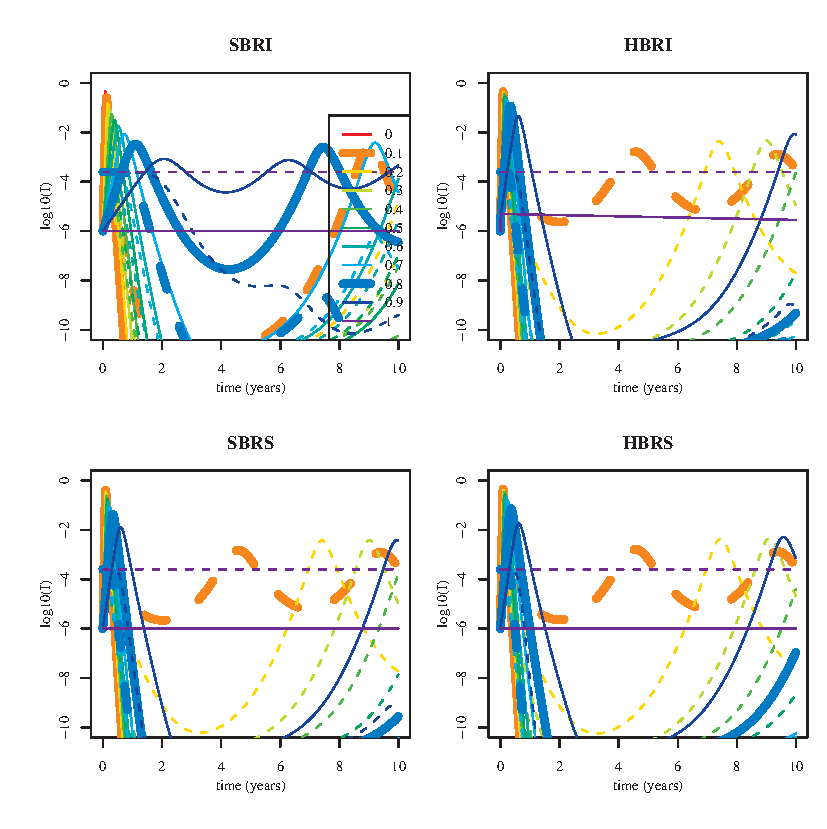
\includegraphics[]{graphs/article1/figure_2.eps}
\end{center}
        \caption{ Transient invasion dynamics for the four two-cluster
          models studied. The decimal logarithm of the proportion of
          infectious hosts for the mutant antigenic cluster (plain
          lines) and for the resident cluster (dashed lines) is
          represented as a function of $\sigma$. Colours correspond to
          different partial cross-immunity ($\sigma$) values: from
          $\sigma=0$ (antigenic shift, no cross-immunity) to
          $\sigma=1$ (antigenic drift, full cross-immunity). Parameter
          values are given in Table \ref{tab:param} (theoretical set).
          Initial conditions are : ${I^1}(0) = {I^1}^*=250.4*10^{-6}$,
          ${I^2}(0)=10^{-6}$.}
\label{fig:deter}
\end{figure}



\begin{figure}[!htbp]
\begin{center}
	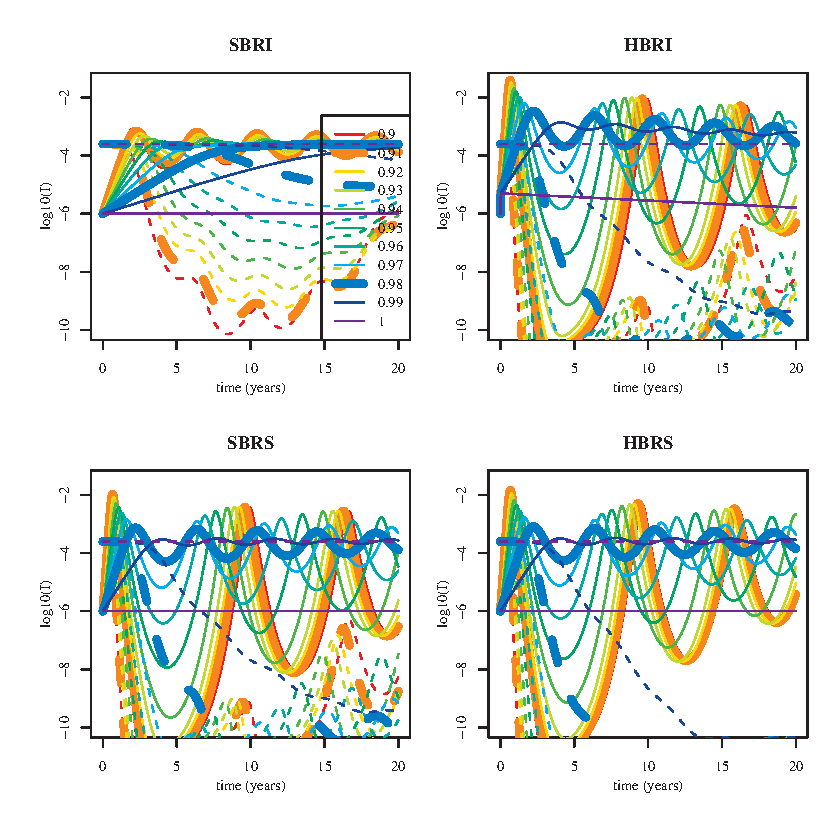
\includegraphics[]{graphs/article1/figure_3.eps}
\end{center}
        \caption{ Detail of figure~\ref{fig:deter}. Partial
          cross-immunity ($\sigma$) values more relevant for gradual
          antigenic drift ($\sigma \in [0.9,1]$).}
	\label{fig:deter_rescaled}
\end{figure}



\begin{figure}[!htbp]
\begin{center}
	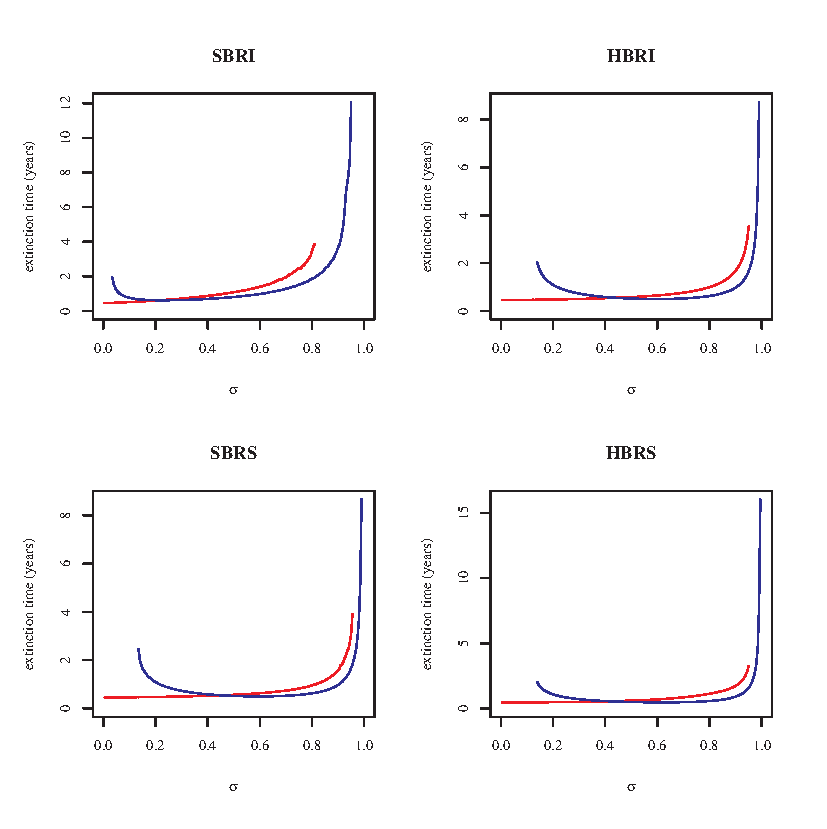
\includegraphics[]{graphs/article1/figure_4.eps}
\end{center}
\caption{ Extinction times of the resident
  antigenic cluster (blue) and of the mutant cluster (red) for the
  four two-cluster models studied. Parameter values are given in Table
  \ref{tab:param} (theoretical set). Initial conditions are :
  ${I^1}(0) = {I^1}^*=250.4*10^{-6}$, ${I^2}(0)=10^{-6}$.}
\label{fig:reinv_theo12}
\end{figure}


For $\sigma \in [0.8, 0.93[$ (corresponding to \citet{Koelle2006}
scale of rare immune escape mutations) in figures~\ref{fig:deter} and
\ref{fig:reinv_theo12} antigenic cluster replacements are possible
only for the $SBRI$ model. The three other models exhibit extinction
of both antigenic clusters.
%
For $\sigma \to 1$ (corresponding to gradual antigenic drift) in
figures~\ref{fig:deter_rescaled} and \ref{fig:reinv_theo12} the $SBRI$
model results in coexistence of both clusters contrary to the three
other models which predict the replacement.
%
For $\sigma \to 0$ (antigenic shifts) in figure~\ref{fig:deter} and
\ref{fig:reinv_theo12} the resident influenza subtype is not
sufficiently affected by the mutant subtype to go extinct and it
survives while the mutant disappears after generating an outbreak.
Note that smaller values of cross-immunity are sufficient for the
$SBRI$ model to drive the resident to extinction
(figures~\ref{fig:deter} and \ref{fig:reinv_theo12}).

In all cases, a proper rescaling of the $SBRI$ model with lower
$\sigma$ values as suggested in Table~\ref{tab:R0} is needed to render
it comparable to the three others models.

\clearpage

\subsubsection{Stochastic  framework}

Simulated trajectories corroborate the trends provided by
deterministic models, especially the particularity of the $SBRI$ model
(figures~\ref{fig:replace}, and Supporting Information~S1).



\begin{figure}[!htbp]
\begin{center}
	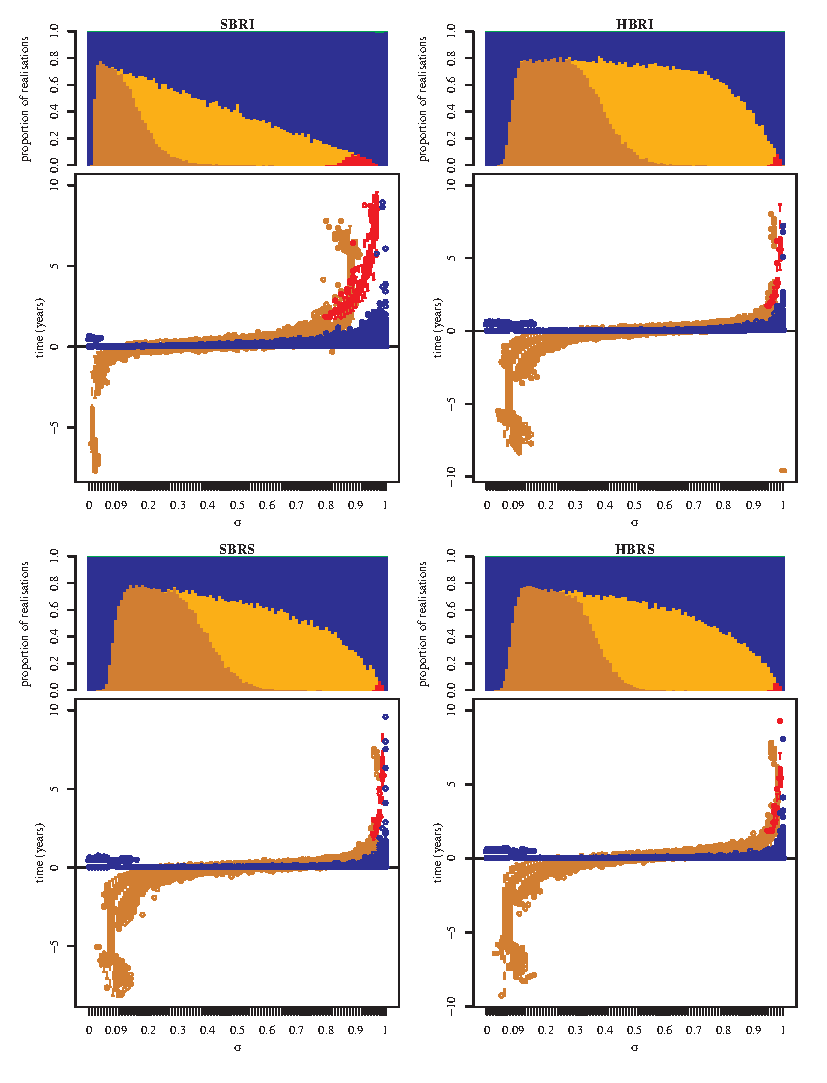
\includegraphics[width= 0.85 \linewidth]{graphs/article1/figure_5.eps}
\end{center}
        \caption{ Outcomes of the transient invasion dynamics based on
          1000 realisations of the four two-cluster stochastic
          models. For each panel, top graphs represent the proportion
          of realisations where, after 10 years: both antigenic
          clusters go extinct, but the mutant goes extinct first
          (brown); both antigenic clusters go extinct, but the
          resident goes extinct first (aborted replacement, orange);
          the resident cluster only goes extinct (successful
          replacement, red); the mutant cluster only goes extinct
          (blue); no cluster goes extinct (coexistence, green). For
          each panel, bottom box plots represent: extinction times of
          the mutant cluster when only this cluster goes extinct
          (blue); extinction times of the resident cluster when only
          this cluster goes extinct (red); the differences between
          extinction times of the mutant cluster and the resident when
          both clusters go extinct (brown and orange). Initial
          conditions: one infected individual with the mutant
          antigenic cluster is introduced in a population where the
          resident cluster is at the deterministic endemic
          equilibrium. The remaining initial conditions are those
          corresponding to the endemic equilibrium of the
          deterministic model and parameter values are given in
          Table~\ref{tab:param} (theoretical set).}
\label{fig:replace}
\end{figure}



The replacement of antigenic clusters following rare mutations with
strong antigenic effect appears to be realistic only in the case of
the $SBRI$ model (figure~\ref{fig:replace}, red bars and Supporting
Information~S1) for which a set of $\sigma$ values consistent with
punctuated immune escape variability exists. For these $\sigma$ values
($\sigma \in [0.8,1[$), a trade-off exists between invasion ability
(that is risks of initial extinction) and risk of epidemic fade-outs
(as described for the evolution of the recovery rate by
\citet{Keeling2000}).  Figure~\ref{fig:replace} shows that the
proportion of initial extinctions, previous to an epidemic caused by
the mutant, decreases as long as the degree of immune escape
($1-\sigma$) increases (blue colour in panel $SBRI$ of
figure~\ref{fig:replace}). At the same time, the proportion of
epidemic fade-outs after replacement increases (orange colour in panel
$SBRI$ of figure~\ref{fig:replace}). Moreover, these results are
consistent with formulas given in Table \ref{tab:R0}, since the
probability of initial extinctions of the mutant cluster is given by
$1/R_0^{inv}$ \citep{Diekmann2000}. For the $SBRI$ model, this
probability increases linearly with $\sigma$ (figure \ref{fig:replace}
$SBRI$, blue bars) whereas for the three other models (panel $SBRI$,
$HBRI$ and $HBRS$ of figure \ref{fig:replace}, blue bars), it remains
uniformly lower and increases as $\frac{1}{R_0+(1-\sigma) (1-R_0)}$
with $\sigma$.

The time necessary to drive the resident cluster to extinction is also
a decreasing function of the immune escape intensity (red boxplot in
panel $SBRI$ of figure~\ref{fig:replace}). For $\sigma \to 1$, transient
coexistence (5 years) of both antigenic clusters is expected before
definitive replacement.

Taken together, the previous results reveal that: \textit{(i)}
antigenic clusters replacement within a serial $SIR$ model is possible
only in the case of a $SBRI$ model; \textit{(ii)} antigenic shift
results in the extinction of both subtypes (brown colour
figure~\ref{fig:replace}, trajectories in Supporting Information~S1)
or of the mutant only (blue colour figure~\ref{fig:replace}).

\subsection{External re-introductions}

\subsubsection{Modelling re-introduction}

In the real world, populations are opened to migration and extinct
clusters can be re-introduced. To complement our results we need to
evaluate the timescales of re-invasion. In particular, we focus on:
\textit{(i)} the robustness of the replacement (i.e. is the resident
able to re-establish in the population due to spatial effects of
re-introduction?); \textit{(ii)} which cluster re-invades first when
both are extinct quasi simultaneously.

Except for initial extinctions, the observed extinctions are mostly
due to deterministic forces of susceptibles depletion and not to
random fluctuations of trajectories evolving close to one individual
(low variances in the box plots of figure \ref{fig:replace}).
Incidentally, the opportunity of a second epidemic after an epidemic
fadeout for the mutant cluster or, the opportunity of re-invasion of
the resident cluster after having been extinct due to the invasion of
the mutant cluster are mostly governed by the deterministic dynamics
of susceptibles renewal \citep{Olinky2008}.

We will thus use deterministic models to compute the average time
necessary before a recurrent epidemic. A simple way to do this is to
consider a constant amount of infectious individuals entering the
population studied. Classically (\textit{e.g.} \citet{Bjornstad2002,
  Keeling2002}) the following scheme has been used:
$$\dot{I_i}=\beta(t) S_i (I_i + m p_i) + ... ,$$
where $m$ is the number of infected individuals imported from outside
(generally $m \sim N^{-1}$) and $p_i$ is the proportion of these
immigrating hosts infected with strain $i$. Note that we do not
consider infecteds from outer regions in the bookkeeping of $I_i$.

From Supporting Information~S1 we can see that the overall pattern
of transient dynamics is not affected by the modelling of external
re-introductions.

\subsection{Re-invasion time-scales}

Figure~\ref{fig:time} reveals that for $\sigma$ values relevant for
punctuated antigenic drift ($\sigma \to 1$), successful replacements
are robust to the re-introduction of the resident antigenic cluster
(\textit{i.e} the re-introduction of the resident cluster does not
lead to an epidemic). In the case of replacements where both clusters
go extinct (the resident being extinct before the mutant) the mutant
cluster re-invades first. This underlines the fact that we face a
replacement. The time until the next epidemic is nevertheless
unrealistically high ($>5$ years) to be consistent with observed
patterns of influenza yearly recurrence in the absence of antigenic
cluster changes.


\begin{figure}[!htbp]
\begin{center}
	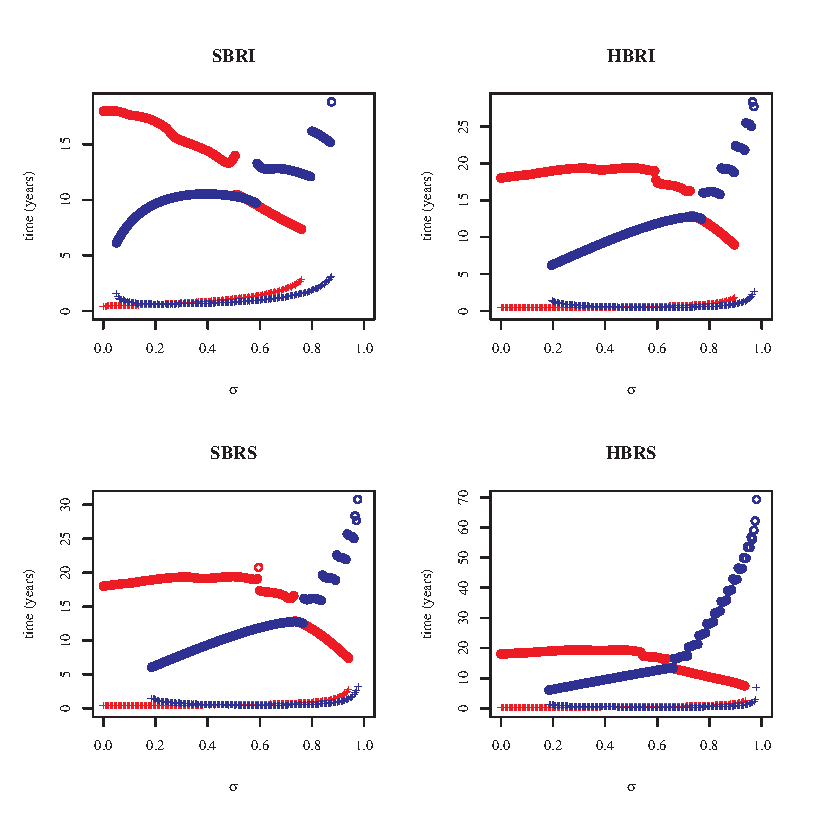
\includegraphics[]{graphs/article1/figure_6.eps}
\end{center}
	\caption{ Extinction and re-invasion times for the four
          two-cluster models in the presence of external
          reintroductions of infectious hosts. (+) represent times
          when a deterministic threshold (equal to $10^{-7}$) for
          extinction is crossed by the trajectories for the resident
          cluster (blue) and the mutant (red) ; (o) correspond to
          times of the first peak after extinction for the resident
          cluster (blue) and times of the second peak of the mutant
          cluster (red). Parameter values are given in Table
          \ref{tab:param} (theoretical set), $mp_i=10^{-8}$. Initial
          conditions are : ${I^1}(0) = {I^1}^*=250.4*10^{-6}$,
          ${I^2}(0)=10^{-6}$}
\label{fig:time}
\end{figure}


For antigenic shifts ($\sigma \to 0$), when both clusters go extinct,
timescales for a recurrent epidemic are also too long to be relevant
(re-invasion time $>10$ years, figure~\ref{fig:time}). In the case
where the invader is able to drive the resident to extinction (that is
for the $SBRI$ model), replacements are not robust to external
re-introduction. The former resident re-appears more than 10 years
before the invader.

\clearpage


\section{Discussion}

Punctuated antigenic evolution is being recognised as an important
mechanism of immune escape in various RNA viruses, but its detection
remains difficult and somewhat uncertain \citep{Cobey2008}. In this
paper we have focused on exploring to what extent the complex
processes shaping influenza dynamics can be approximated by a minimal
serial $SIR$ system, emphasising rare mutations with strong antigenic
effects. According to our results (figure~\ref{fig:deter},
\ref{fig:deter_rescaled}), punctuated immune escape results in a high
depletion of susceptibles in $SBRS$, $HBRS$ and $HBRI$ models. As a
consequence, recurrent epidemics during consecutive years are rendered
impossible even with reintroductions. However, data clearly suggest
that several recurrent epidemics of the same new mutant cluster can
follow the replacement of the resident cluster by the new one. For
instance, following its invasion, Beijing/1993 (BE93) cluster has
provoked epidemics of 1992-1993, 1993-1994, 1994-1995 and 1995-1996
seasons in New York state before being replaced by Wuhan/1995
(WU95)-like viruses \citep{Rambaut2008}. Such dynamics can only be
reproduced by the \textit{SBRI} model because it produces
comparatively slower invasion dynamics and fewer susceptible
depletion. A minimal serial \textit{SIR} theory is thus supported only
within the $SBRI$ framework.

In the following, we review the processes that makes the $SBRI$ model
different from \textit{HB} or \textit{SB} models with \textit{RI}
assumption. We then provide elements pointing out that these processes
direct towards a biologically problematic description of
cross-immunity. Finally, we provide arguments supporting the idea
already evoked by \citet{Koelle2006} that a sequential $SIR$ model
requires within antigenic cluster gradual antigenic drift and that
this process should be part of a minimal theory for influenza dynamics
at the population level.

\subsection{Is the $SBRI$ model particularly appropriate?}

One of the important aspects of influenza dynamics is the
cross-immunity represented here by the parameter $\sigma$ which
measures the antigenic distance between two strains, regardless of the
modelling framework. Here, the range of variation of $\sigma$ was the
same for the four models and was chosen according to
\citet{Koelle2006}. This allowed direct comparison between the four
models.

Our results reveal that the similar dynamics are generated for
significantly higher values of $\sigma$ in the case of the $SBRI$
model than for the other three models (Table~\ref{tab:R0}). This
difference in behaviour is due to the fact that in the $SBRI$ model,
individuals that have been infected with cluster $i$ can be reinfected
by the same cluster. These reinfected hosts will not be infectious
(because of the \textit{RI} assumption) but may enhance their immunity
to cluster $j$ (figure~\ref{fig:models}, middle).
%%
In equation~\eqref{eq:sbric} repeated infections corresponds to the
terms $- \beta_i R_i I^i$. $\sigma$ percent of these hosts acquire
immunity to strain $j$, progressing to the $R_{ij}$ status whereas the
remaining $(1- \sigma) \beta_i R_i I^i$ hosts keep the $R_i$ status.
As noted by \citet{Kryazhimskiy2007}, such cross-immune enhancement is
impossible in the $SBRS$ model because by construction of this latter
model $R_i$ hosts are no more susceptible to cluster $i$ and cannot be
reinfected.

In the context of influenza, cross-immune enhancement as provided by
the $SBRI$ model appears to contradict established theory for
immunodominance, cross-reactivity and interference (see
\citet{Frank2002} for a review).
%
For sequential infections, a key question is to determine whether a
new infecting strain is sufficiently different from a previously
encountered strain to consider that a new primary response would be
mounted by the immune system instead of a secondary response.
%
In our model, we considered that independent primary responses were
mounted for the different antigenic clusters. Strains belonging to
cluster $j$, were supposed sufficiently different from strains
belonging to cluster $i$ not to interact with memory cells supporting
immunity toward strains of cluster $i$. The reinfection then results
in the production of $R_{ij}$ hosts in both \textit{SBRS} and
\textit{SBRI} models.
%
For the case of reinfection of $R_i$ hosts with closely related
strains belonging to cluster $i$ (possible only for the \textit{SBRI}
model), one can reasonably assumes that such strains are sufficiently
closed to interact with the memory cells (otherwise they would belong
to cluster $j$). In this case, according to \citet{Frank2002}, we can
expect a sequential effect called original antigenic sin, well known
for influenza \citet{Francis1953, St1966, Janeway1999}. Within original
antigenic sin, a strong response against a previously recognised
epitope represses the response against the changed epitope. As the
\textit{SBRI} model assumes a strong and immediate response toward the
previous epitope (hosts reinfected with a virus from an identical
cluster are no longer infectious), the rapid response from memory
cells may keep viral load below the threshold required to stimulate
naive B or T cells (other processes are also possible \citep{Janeway1999}).

Given these mechanisms, the cross-immune enhancement provided by the
$SBRI$ model should be considered as an overestimation bias of
immunity and proper rescaling of $\sigma$ should be done before using
the $SBRI$ model in the context of influenza.

\subsection{Toward a minimal theory for influenza}

Except for the biologically problematic $SBRI$ model, our results
stress that the occurrence of new antigenic clusters resulting from
immune escape mutations rapidly induces important depletion of
susceptibles. This depletion results in an extinction of the invading
antigenic cluster and this phenomenon is robust to reintroductions
(figure~\ref{fig:deter}, \ref{fig:deter_rescaled} and
\ref{fig:time}). Thereafter, we propose processes that can
favour the replacement of the resident by the mutant as observed in
data.


\subsubsection{Gradual antigenic drift within antigenic clusters}

\citet{Goekaydin2007}, have considered a model that incorporates
gradual antigenic drift within antigenic clusters. They have assumed
that within cluster evolution results in a diversity of strains that
renders immunity to an antigenic cluster only partial. Partial
immunity has been modelled by a $SIRI$ model \citet{Gomes2004a},
allowing reinfection at a slower rate. \citet{Goekaydin2007} have
shown that reinfections define a reinfection threshold
\citet{Gomes2004a, Gomes2005} that plays a central role in determining
the outcome of the invasion by a new antigenic cluster. Reinfection
determined by gradual antigenic drift therefore appears to be central
for successful antigenic cluster replacement as observed in data.
Contrary to \citet{Goekaydin2007} claims that no antigenic cluster
replacement can occur within $SIR$ models, we have shown that this
could be the case with $SBRI$ models. However, since the $SBRI$ model
is biologically problematic, it still remains to be tested whether
$SIRI$ or $SIRS$ models would best describe drifting antigenic
cluster.

Contrary to the $SIRI$ model which assumes that strains diversity
within a given antigenic cluster results in partial immunity, the
$SIRS$ model considers that within antigenic clusters evolution
results in a progressive loss of immunity \citep{Pease1987}. Our
investigation of the transient dynamics of drifting cross-reactive
clusters modelled by $SIRS$ models as described in
figure~\ref{fig:model_sirs} and section 4 of Supporting Information~S1
reveals that small amount of gradual antigenic drift can favour
antigenic replacement over epidemic fadeout (figure
\ref{fig:within_drift} and Supporting Information~S1). Within cluster
gradual antigenic drift, whether included in $SIRS$ or $SIRI$ models
can therefore turns epidemics fadeout of the mutant cluster into a
successful replacement.

\begin{figure}[!htbp]
\begin{center}
  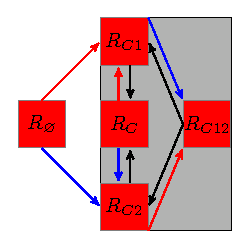
\includegraphics[width=0.3\linewidth]{graphs/article1/figure_7.eps}
\end{center}
\caption{ An history based model for drifting co-circulating
    cross-reactive antigenic clusters. The viruses are supposed to
  contain two antigens: a conserved antigen, shared by strains of the
  resident and the mutant antigenic cluster and a specific antigen,
  specifying each cluster. Naive hosts acquire immunity to both
  conserved and specific part ($R_{Ci}$) resulting in full protection
  toward strains of cluster $i$. Within cluster antigenic drift
  affects only the specific antigen resulting in $R_{Ci} \to R_C$
  transitions at a rate governed by parameter $\gamma$. The shared
  conserved antigen confers partial protection reducing the
  probability of reinfection by a factor $1-\sigma$. Red (blue) arrows
  represent infection by cluster 1 (2). Black arrows represent within
  cluster antigenic evolution. A full description of the assumptions
  leading to this model is provided in section 4 of Supporting
  Information~S1. These hypotheses also enable to recover the model of
  \cite{Goekaydin2007} and therefore render the two frameworks ($SIRI$
  and $SIRS$ within cluster antigenic drift description) readily
  comparable.}
  \label{fig:model_sirs}
\end{figure}



\begin{figure}[!htbp]
\begin{center}
  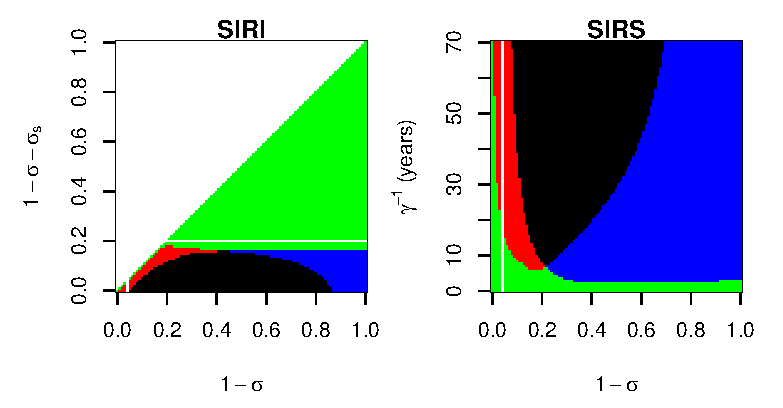
\includegraphics[width=0.7\linewidth]{graphs/article1/figure_8.eps}
\end{center}
  \caption{ Effect of the introduction of within cluster gradual
    antigenic drift on the outcome of the invasion of a new antigenic
    cluster. Comparison of the $SIRS$ model (right) described in
    figure~\ref{fig:model_sirs} and Supporting Information~S1 with the
    $SIRI$ model of \cite{Goekaydin2007} (left). x-axis scale the
    amount of immune escape achieved by the mutant antigenic cluster.
    y-axis represent a measure of within cluster antigenic drift (see
    Supporting Information~S1 for details). Colours: both antigenic
    clusters go extinct (black), the resident cluster only goes
    extinct (successful replacement, red); the mutant cluster only
    goes extinct (blue); no cluster goes extinct (coexistence, green).
    Extinction threshold is set at $N=10^{-7}$. Parameter values are
    given in Table \ref{tab:param} (theoretical set). The horizontal
    white lines of the left graphs situates the reinfections
    thresholds of the $SIRI$ models
    ($1-\sigma-\sigma_s=\frac{1}{R_0}$). The vertical white lines set
    the highest immune escape intensity ($1-\sigma$) for which the
    same model without within cluster antigenic drift predicts
    replacements.}
\label{fig:within_drift}
\end{figure}


Introducing gradual antigenic drift in a minimal model for influenza
also allows to reduce the high critical community size needed to
ensure the persistence of a resident antigenic cluster. A small rate
of gradual antigenic drift have a dramatic effect on the CCS of a
resident antigenic cluster reducing the CCS from 10 millions to 1-2
millions (Supporting Information~S1). CCS closer to one million
renders stochastic effect (such as noise induced temporal asynchrony
\citep{Kamo2002}) important to consider as they could potentially
facilitate coexistence.

These theoretical results corroborate \citet{Finkenstaedt2005},
\citet{Shih2007} and \citet{Suzuki2008} analysis of antigenic drift at
the population level.  \citet{Finkenstaedt2005} have estimated
baseline antigenic drift rate from influenza like illness data using a
model allowing sudden discrete changes and have shown that it was
significantly different from zero. \citet{Shih2007}, using a method
with a higher power of detection of positive selection than previous
studies, have shown that within antigenic cluster change could be more
important than traditionally (\textit{e.g} \citet{Wolf2006}) believed.

Gradual antigenic drift should thus be part of a minimal model for
influenza A along with punctuated immune escape.

%\clearpage

\subsubsection{Functional constraints}

Functional constraints are well established for influenza A
\citep{Rambaut2008, Gog2008, Du2008}. For instance, it has been
established that cooperative activities of both HA and NA are critical
for influenza virus infection and release \citep{Wagner2002}.
Functional constraints can induce a fitness cost associated to an
antigenic escape mutation. Lower fitness of the mutant cluster could
be beneficial for the replacement dynamics as by decreasing the
strength of the initial invasion, functional constraints could also
decrease the risk of epidemic fadeout and long refractory periods that
follow high depletion of susceptibles. %
A simple way to handle functional constraints is to consider a
relation between the mutant cluster transmission rates ($\beta_{mut}$)
and its ability to escape previous immunity (governed by $\sigma$).
Without loss of generality, functional constraint can be introduced by
lowering $\beta_{mut}$ (assuming $\beta_{mut}=\alpha \beta_{res}$ with
$\frac{1}{R_0^{res}} \leq \alpha \leq 1$) to ensure that $1 \leq
R_0^{mut} \leq R_0^{res}$. Using section~Results results we can
calculate the threshold value of $\sigma$, equal to $\sigma^*$,
necessary for the antigenic cluster invasion. In case of both $HB$ and
$SBRS$ models, the threshold is defined by $\sigma < \frac{\alpha
  R_0^{res}-1}{\alpha (R_0^{res} -1)}$. Functional constraints can
explain why immune escape mutations do not generate unrealistic high
epidemics (Supporting Information~S1). To compare our results to
\citet{Koelle2006} model, we have neglected such constraint but they
should be considered in further investigations. Such inclusion would
need to incorporate compensatory mutations \citep{Du2008} to restore
original function and re-increase the impaired $\beta_{mut}$.
\\

\subsubsection{Multiple infections before acquiring immunity}

As we have shown through simulations (figures~\ref{fig:deter},
\ref{fig:reinv_theo12} and \ref{fig:replace}), subtype replacement (as
a consequence of antigenic shifts) appears impossible except in the
case of the questionable $SBRI$ model. This is contrary to what have
been observed during previous 1957's Asian flu and 1968's Hong Kong
flu pandemics \citep{Earn2000}. This lack of realism was reported by
\citet{Ferguson2003} in case of history based models and had been
partially solved by including temporary cross-immunity
\citep{Webster1992}. However, other proposals that temporary
cross-immunity could also be relevant. For instance, by using data of
the first introduction of H3N2 type A influenza on the island of
Tristan da Cunha in 1971, \citet{Mathews2007} show that two epidemics
separated by 20 days only have affected the population and most of the
hosts have been infected twice. This is different from the
conventional knowledge of influenza immunology and suggests that
multiple infection could be necessary before developing long term
immunity. This creates far more susceptible individuals than expected
from our models and greatly favours the persistence of the new
subtype. It remains to be tested whether the persistence of the new
subtype is sufficient to drive the resident subtype to extinction.
Concerning epidemic influenza, the need to incorporate multiple
infection before the acquisition of immunity deserves further
attention.
\\

\vspace{1cm}

As a last point, \citet{Recker2007} have reopened a theory on
influenza antigenic evolution dominant in 1960 \citep{Francis1960}.
Within this theory, the virus population is characterised by a limited
set of antigenic types, all of which may be continuously
(re-)generated from preexisting strains. \citet{Recker2007} have shown
that sampling from a population where a limited set of antigenic types
describe complex dynamics can reproduce the specific patterns of
antigenic cluster succession revealed by \citet{Smith2004} analysis.
This view offers an alternative explanation to the sequential
antigenic drift scenario examined in this paper. Recent data, analysed
by phylogenetic and coalescent based approaches, strongly suggest that
influenza A dynamics is part of a source-sink system where the source
could be a reservoir of a limited set of antigenic types
\citep{Alonso2007a, Nelson2007b, Holmes2005, Nelson2006, Viboud2006,
  Rambaut2008, Russell2008}. However, it remains to be seen to what
extent restriction of viral genetic diversity could be achieved by
\citet{Recker2007} model. This model strongly depends on antigenic
recycling to justify the low dimensionality of the phenotype space,
but antigenic recycling does not seem to be supported by current data
\citep{Minayev2008, Minayev2009}.\\

\vspace{1cm}


In conclusion, our findings finally suggest the importance of gradual
antigenic drift for epidemic dynamics even in the presence of
punctuated immune escape. Our results indicate that status based model
with reduced infectivity assumption can have profound consequences on
the transient dynamics of strains invasion. In case of influenza, this
model should be used with caution as it includes biologically
unsupported processes that can induce serious bias.


% Do NOT remove this, even if you are not including acknowledgments
\section{Acknowledgments}

The authors are grateful to Mercedes Pascual for helpful discussions.




%%% Local Variables: 
%%% mode: latex
%%% TeX-master: "../../phD"
%%% End: 


\clearpage
\newpage
\thispagestyle{empty}
\null
\newpage

%
%\clearpage
%\documentclass[11pt,a4paper]{scrartcl}
\documentclass[12pt]{article}

\usepackage[top=2.0cm, right=2.0cm, left=2.0cm, bottom=2.0cm]{geometry}
\usepackage[utf8]{inputenc}
\usepackage[UKenglish]{babel}
%tableau
\usepackage{array, multirow}
%graphs
\usepackage{graphicx}
\usepackage{float, caption}
\usepackage{amsmath,amssymb,mathrsfs}
\usepackage{natbib}
%pour avoir la biblio avec nom d'auteur et année dans le texte
\bibpunct{(}{)}{;}{a}{,}{,}
%pour avoir les reference entre parenthese et en cas de ref multiple séparé par des ;
\sloppy 
%utiliser ca si latex trop exigeant en largeur ligne


\title{Gradual antigenic drift explains complex reccurent pattern of human influenza A}

\author{Sébastien Ballesteros$^{1,*}$, Anton Camacho$^{1}$, Elisabeta Vergu$^{2}$, Bernard Cazelles$^{1,3}$}


\date{}

\begin{document}

\maketitle

$^1$UMR 7625  (UPMC, ENS, AgroParisTech, CNRS), Ecole Normale Supérieure, Unit of Eco-Evolutionary Mathematics,  46 rue d'Ulm, F-75230 Paris Cedex 05, France. \\
$^2$~INRA, UR341 Mathématiques et Informatique Appliquées, F-78352 Jouy en Josas, France \\
$^3$~IRD UR GEODES, 93142 Bondy, France

~\\
$^*$\textit{Corresponding author}:  \\
E-mail: sebastien.ballesteros@biologie.ens.fr

\abstract{}


To what extent epidemic peaks amplitude variability can be due due non-linear dynamics alone ?

To test between a continuous antigenic drift scenario and a punctuated evolutionary one, we have developed a simple model, the perturbated SIRS model.

Results : 
discrete evolution (burst of positive selection) are not correlated with peak variability.

calculer la correlation entre la date du peak et la date de la mutation a grand effet
tracer ce coeff en fonction de l'intensité du forcage saisonier et de la variance de la loi normale

construire un test statistique pour voir si l'effet est significatif.


idée en vrac mais bien !!!:
il nous faut determiner l'amplitude de l'immune escape.
une facon de calibrer: regarder la perturbation d'un modele SIRS voir a partir de quelle niveau on genere des peaks plus grand...

on peut faire le calcul avec comme ordre de grandeur la valeur de l'equilibre endemique
calculer l'ecart entre le peak et l'equilibre endemique

~ \\
\textit{Keywords}: \\
influenza, punctuated immune escape, status based model, history based
model, reduced susceptibility, reduced infectivity

\section{Intrinsic period of oscillation in a SIRS model}
Assuming a constant hosts population size, the $SIRS$ model is:

\begin{align}
  \frac{dS}{dt} & = -\beta S I + g (1-S-I)\\
  \frac{dI}{dt} & = \beta S I - \nu I\\
\end{align}

The $SIRS$ model can be simplified, resulting in a
reduction in the number of parameters. Measuring time
in units of duration of infection, $t'=t \nu$, we get the non dimensional system:

\begin{align*}
  \frac{dS}{dt'} & = -R_0 S I + e (1-S-I)\\
  \frac{dI}{dt'} & = R_0 S I - I\\
\end{align*}

With $R_0=\frac{\beta}{\nu}$ and $e=\frac{g}{\nu}$.

The model has two possible steady states
\begin{itemize}
\item Disease-free equilibrium: $S=1$, $I=0$
\item Endemic equilibrium: $S=\frac{1}{R_0}$, $I=\frac{e-e/R_0}{1+e}$.
\end{itemize}

The stability of the endemic equilibrium is determined by the
eigenvalues of the Jacobian matrix:
$$J=
\begin{pmatrix}
  -R_0 I -e & -R_0 S -e\\
  R_0 I & R_0 S-1 \\
\end{pmatrix}$$
Evaluated at the endemic equilibrium it results in:
$$\begin{pmatrix}
\frac{e(1-R_0)}{1+e} & -1-e \\
\frac{e(R_0 -1}{1+e} & 0 \\
\end{pmatrix}$$

The eigenvalues are solution of
\begin{align*}
\det{J-\lambda I_2} & = 0 \\
\lambda^2 - \frac{e(1-R_0)}{1+e} \lambda +e(R_0-1) & =0\\
\end{align*}

A straightforward calculation shows that the discriminant is negative and the eigenvalues thus complex:
$$\lambda_i = \frac{\frac{e(1-R_0)}{1+e} \pm i \sqrt{4 e (R_0-1)-\frac{e^2(R_0-1)^2}{(1+e)^2}}}{2} $$

The period of the dampened oscillations is given by 
\begin{align*}
  T & =2\pi \frac{1}{\Im{\lambda}} \\
& = 2\pi \sqrt{\frac{4}{4 e (R_0-1)-\frac{e^2(R_0-1)^2}{(1+e)^2}}} \\
\end{align*}

In the natural timescale, the period is divided by $\nu$
As $e \to 0$, the period can be simplified in :
$$T=2 \pi \sqrt{\frac{DL}{R_0-1}}$$ expressed in natural timescale with $D=1/\nu$ and $L=1/g$.

\section{seasonal forcing}

\subsection{Floquet}

We now consider the following non autonomous system:

\begin{align*}
  \frac{dS}{dt} & = -\beta(t) S I + g (1-S-I)\\
  \frac{dI}{dt} & = \beta(t) S I - \nu I\\
\end{align*}

with $\beta(t)=\beta_0(1+e \cos(2 \pi t))$.



For positive initial conditions and some parameters values, the seasonally forced $SIRS$ model admits a stable periodic solution of period T.
We will label limit cycle solutions by $\mathbf{\bar{x}}(t) = (\bar{S}(t), \bar{I}(t))$ in the following calculations and have $\mathbf{\bar{x}}(t + T ) = \mathbf{\bar{x}}(t)$ for all times, t. 
The curve, $\mathbf{\bar{x}}(t)$, cannot be calculated in closed form. However good estimates can be obtained via numerical integration of Eq. (1).

In order to study stability, we now consider a dynamical path beginning close to, but not on, the limit cycle, $\mathbf{\bar{x}}(t)$. If the limit cycle solution is stable then the difference between this path and the geometric curve of the limit cycle will decay as time progresses.  Similarly to the expansion about a fixed point, we can write this difference as $\epsilon \mathbf{\xi}(t) = \mathbf{x}(t) - \mathbf{\bar{x}}(t)$  where, again, $\epsilon$ expresses our anticipation that the deviation from the limit cycle is small. Expanding in powers of $\epsilon$ and letting $\epsilon \to 0$, one then finds that the time evolution of $\mathbf{\xi}(t)$ takes on the linear form, $\frac{d\mathbf{\xi}}{dt} = \mathbf{A}(t) \mathbf{\xi}$, where the matrix $\mathbf{A}(t)$ is the Jacobian matrix evaluated at the limit cycle. 
Therefore, due to the periodic nature of $\mathbf{\bar{x}}(t)$, all elements of $\mathbf{A}(t)$ are periodic.

An analytical tool to characterize the stability or otherwise of limit cycle solutions is Floquet theory, the mathematical theory of linear differential equations with periodic coefficients. Since, we have $\mathbf{A}(t+T)= \mathbf{A}(t)$, Floquet theory is applicable. In our case, T is the period of the mean-field limit cycle under consideration.
The general solution of
$$\frac{d\mathbf{\xi}}{dt} = \mathbf{A}(t) \mathbf{\xi}$$
takes the form:
$$\mathbf{\xi}(t) = \sum_{i=1}^n c_i e^{\mu_i t} \mathbf{p}_i(t)$$
$\mu_i$ are complex numbers called characteristic or Floquet exponents.
Floquet exponents can be calculated numerically by solving the matrix differential equation
$$\frac{d\mathbf{X}}{dt} = \mathbf{A}(t) \mathbf{X}$$
over one period (from $t=0$ to $t=T$) with the identity matrix as an initial condition ($\mathbf{X}(0)=\mathbf{I}$)
The matrix $\mathbf{X}(T)$ is known as a fundamental matrix.
Floquet multipliers, $\rho_i$ are the egeinvalues of $\mathbf{X}(T)$. 
$\rho_i$ are also the eigenvalues of the (linear) Poincaré map $x(t) \rightarrow x(t+T)$
From $\rho_i$, Floquet exponents, $\mu_i$ are calculated as $\mu_i= \frac{\ln(\rho_i)}{T}$

In term of Floquet multipliers, the general solution is
$$\mathbf{\xi}(t) = \sum_{i=1}^n c_i e^{\frac{\ln(\rho_i)}{T} t} \mathbf{p}_i(t)$$
expressing $\rho_i= |\rho_i|e^{i \arg(\rho_i)}$ we have:
$$\mathbf{\xi}(t) = \sum_{i=1}^n c_i e^{(\frac{\ln(|\rho_i|)}{T}+ i \frac{\arg(\rho_i)}{T}) t} \mathbf{p}_i(t)$$
that gives the damping rate and oscillation period

if $\Re(\rho_i)>0$ $\arg(\rho_i)= \arctan(\frac{\Im(\rho_i)}{\Re(\rho_i)})$
else $\arg(\rho_i)= \pi- \arctan(\frac{\Im(\rho_i)}{\Re(\rho_i)})$

\subsection{larger perturbation}

\subsection{Invasion orbit}

\end{document}



%%% Local Variables:  %%% mode: latex %%% TeX-master: t %%% End: 


\clearpage
\newpage
\thispagestyle{empty}
\null
\newpage

%
%\clearpage
\chapter{The transition from invasion to persistence for influenza
  antigenic units}


Sébastien Ballesteros$^{1,*}$,
Anton Camacho$^{1}$,
Elisabeta  Vergu$^{2}$,
Bernard Cazelles$^{1,3}$

\vspace{2cm}

$^1$UMR 7625  (UPMC, ENS, AgroParisTech, CNRS), Ecole Normale
Supérieure, Unit of Eco-Evolutionary Mathematics,  46 rue d'Ulm,
F-75230 Paris Cedex 05, France.
\\
$^2$~INRA, UR341 Mathématiques et Informatique Appliquées, F-78352
Jouy en Josas, France
\\
$^3$~IRD UR GEODES, 93142 Bondy, France
\\
$^*$\textit{Corresponding author}:
E-mail: sebastien.ballesteros@biologie.ens.fr


\tikzstyle{naif} = [draw, fill=white, rectangle, minimum height=2em, minimum width=3em]
\tikzstyle{expo} = [draw, fill=blue, circle,minimum height=2em]
\tikzstyle{mut} = [draw, fill=red, circle,minimum height=2em]


\section*{abstract}

We introduce a general framework to capture the dynamics of partially
cross reactive influenza subtypes or antigenic cluster subject to
gradual antigenic drifts. We assume that antigenic unit (influenza A
subtype or antigenic cluster) are produced during discrete events
(antigenic shift or cluster transition) that determines their
antigenic distance. Antigenic distance then remains constant despite
within unit antigenic drift. The implicit representation of within
unit gradual antigenic drift added to the fact that we track the tempo
of antigenic change instead of the pathogen's genetic change allows to
consider only a limited number of antigenic unit at any time. These
simplifications render possible to use multi-strains model where the
number of compartments grows exponentially with the number of
antigenic units overcoming the need to use restrictive hypothesis to
simplify model complexity. Using this framework, we first show how the
presence of gradual antigenic drift within antigenic unit induces the
existence of a determinist threshold that governs the invasion ability
of new drifting antigenic units. We then characterise the conditions
leading to replacement of antigenic units as observed in data using a
realistic worldwide stochastic metapopulation model.
%
With this framework our results reveal that realistic parameter values
for immune escape lead to unrealistically high epidemics followed by
too long refractory periods.  
%
A good agreement between simulations and data can be obtained by
assuming an associated fitness cost to immune escape or by including a
mechanism of immune boosting where exposed individuals that do not
contract infection nevertheless gain a temporary period of full
cross-protection.
%
Such a cross-immune boosting appear to be a common point shared by
models able to reproduce successful antigenic units replacements but
its necessity could be an artifact of global mixing assumption.

\vspace{2cm}


\textit{Keywords}: \\
influenza, punctuated immune escape, antigenic drift, invasion threshold

%\tableofcontents

\section{Introduction}

Past influenza A pandemics in human have been marked by characteristic
patterns of replacement where the new invading subtype successfully
establish in the human population while driving the preexisting
subtype to extinction.
%This was the case during 1918 Spanish influenza where
%H1N1 replaced a supposed H3N8 subtype dating from 1900, 1957 Asian
%influenza with H2N2 replacing H1N1 and 1968 Hong Kong influenza with
%H2N2 being replaced by H3N2. 
This happened three times since 1918 when ``Spanish'' influenza H1N1
replaced a supposed H3N8 subtype dating from 1900. H1N1 was then
replaced by Asian influenza H2N2 in 1957 and finally this latter was
replaced by Hong Kong influenza H3N2 in 1968. Coexistence of two
influenza subtypes was only recently observed following the accidental
reintroduction of H1N1 in 1977 \citep{Kilbourne2006, Zimmer2009}.
%
Human A influenza virus can therefore be considered as a perturbed
system prevented from reaching an evolutionary equilibrium with their
hosts by an irregular infusion of avian virus genes into the human
virus gene pool \citep{Webster1992}. The current pandemics of new
animal origin H1N1 virus (naoH1N1) constitutes a prominent example of
such perturbation.
%

%
% This pattern of subtype replacement observed for influenza A in
% human is in strong contrast with the situation occuring in aquatic
% birds where 16HA and 9NA coexists.

Within a given influenza subtype (IS), intense selection from the host immune system
also results in continuous replacement of circulating strains with new
variants able to re-infect previously immunized hosts.
%immune to earlier types. 
This antigenic drift results in a strong temporal signature in HA
(influenza main antigen) phylogeny with high rates of lineages
extinctions so that genetic diversity at any time is limited
\citep{Fitch1997}. By contrast, the phylogeny of influenza type B,
which affects only humans and is not perturbed by frequent antigenic
shifts episodes \textit{i.e.} introduction of a new subtype in the
human population from an animal reservoir (\citet{Webster1992}),
exhibits greater branching events \citep{Hay2001}. Influenza B
currently possesses 2 lineages (B/victoria and B/Yamagata) that have
been coexisting with frequent reassortments since the early 80's
\citep{Lin2004}.

The dynamics of influenza antigenic unit (IAU) replacements is
therefore a key process of influenza epidemiology and evolution and
numerous studies have tried to determine the key factors involved in
IAU replacements or coexistence whether it be during pandemic shifts
or seasonal influenza antigenic drift.


Using a computationally intensive individual based model,
\citet{Ferguson2003} were able to reproduce both the slender
phylogenetic tree of influenza A HA and the pattern of subtype
replacement observed during pandemics. \citet{Ferguson2003} have shown
that replacement was strongly dependent on the presence of a
short-lived strain-transcending immunity within and between subtypes,
which acts as a density dependant factor. Pattern more reminiscent to
influenza B were obtained by reducing both the intensity of partial
cross-immunity and the rate of mutation with few effects of the basic
reproductive number $R_0$.
%
\citet{Andreasen2006} recovered most of \citet{Ferguson2003} results
using an analytical model. Under \citet{Andreasen2006} model, partial
cross-immunity alone is sufficient to prevent branching events for low
$R_{0}$ values. However, for a fixed level of cross-immunity
intensity, branching events are more likely as $R_{0}$ increases and a
temporary strain-transcending immunity becomes necessary to reduce
diversity as $R_{0}$ takes realistic values.

Recently, \citet{Koelle2006} and \citet{Koelle2009} have introduced an
efficient framework to model rapidly evolving pathogens by focusing on
the tempo of antigenic change instead of the pathogen's genetic
change. At the heart of this framework is the recognition that groups
of strains with the same antigenic properties form a limited number of
antigenic clusters (AC) emerging and replacing each other every 1 to 8
years \citep{Smith2004}. Within a given AC gradual antigenic drift
takes place and strain diversity increases \citep{Shih2007,
  Suzuki2008, Russell2008}. However, AC transitions induce important
selective sweeps that restricts previously established diversity. In
this context, \citet{Koelle2006} showed that temporary
strain-transcending immunity is unnecessary to restrict the diversity
of HA within H3N2 subtype evolution. \citet{Koelle2006} and
\citet{Koelle2009} also offered a mechanism to explain the different
pattern of coexistence observed for influenza type B and A/H1 by
reporting more coexistence events instead of sequential replacement
for $R_0$ values smaller or greater than 4-6.

One of the main issue with \citet{Koelle2006} model is that it has
been framed within a status-based framework with the assumption that
cross-immunity acts by reducing infectivity ($SBRI$ model). This
combination of hypothesis have been reported to result in potentially
important overestimation bias of immunity in the context of influenza
that could favour otherwise impossible AC replacement
\citep{Ballesteros2009}.

Here, we introduce a general framework more appropriate than the
$SBRI$ model to capture the outcomes of the invasion of partially
cross-reactive IAU subject to gradual antigenic drift. As previously
stated, these IAU appear to result from rare mutations (or
re-assortments) with strong antigenic effects in the case of AC or
from antigenic shifts in the case of IS. In between these punctuated
events, gradual antigenic drift occurs (\citep{Shih2007, Russell2008,
  Suzuki2008}) but we assumes that it does not affect cross-reactivity
of the different IAU so that the antigenic distance between antigenic
units remains constant despite within unit evolution. This internal
treatment of gradual antigenic drift leads to greatly simplify model
complexity and enable to use models where complexity scales
exponentially with the number of IAU.

We first show how the presence of gradual antigenic drift within IAU
induces the existence of a deterministic threshold that governs the
invasion ability of new drifting antigenic units.

We then use the previously defined framework to study the transient
dynamics from invasion to persistence for new emerging drifting IAU
focusing only on partial cross protection. Simple patterns are first
characterised with a two-antigenic units model and the prediction of
this simple analysis is complemented by simulation of a multi drifting
IAU model in a realistic worldwide metapopulation context.

Finally, we consider the effect of a period a temporary
strain-transcending immunity and discuss the key processes that appear
to shape influenza phylodynamics and pandemics patterns.





%limit koelle: pandemics limit ferguson unclear whether or not these
%models generate antigenic clusters.


%Ferguson tree more similar to B require reducing both intensity of
%cross immunity and rate of mutation
%fergusson cross immunity linear 0.99 a besoin de 2 change pour
%commencer a diminuer lineairement jusqu'a 0.25
%pour que coexist; linear 0.8 besoin de 1 changementpour que commence a
%diminuer -> 0.5

%Koelle sigmaij=0.85^distance




%Various processes can results in interaction between the antigenic
%unit. Long lasting cross reactive antibodies can results in partial
%cross protection for different antigenic unit. Cellular immunity
%targeted to conserved part of influenza also play an important role
%and has been postulated to be the support of a period of temporary
%full cross immunity.

%In case of antigenic clusters, the characteristic antigenic
%property can be related to the fact that the antigen three dimensional
%structure remains approximately conserved or that the relationship
%between the virus and the host remains unchanged
%\citet{Blackburne2008}. Influenza subtype also represent a general
%characteristic. 


%\cite{Viboud2005} smoldering pandemics liens avec H2N2 l'année
%précedente =>importance des conditions initiales.


\section{A general framework for co-circulating cross-reactive
  IAU subject to gradual antigenic drift}

History based or status based model can be used to model
co-circulating IAU \citep{Gog2002a}. However, as we show in the
appendix, generalising classical status based model (\textit{e.g}
\citet{Gog2002a} or \citet{Gog2002}) to include within IAU antigenic
drift tuns to be problematic, leading to difficult biological
interpretations as well as overestimation of cross-immunity.

In this context, history-based framework appears to be a more natural
alternative where gradual antigenic drift within IAU can be introduced
in two ways, both biologically relevant. A first way was previously
explored by \citet{Goekaydin2007} who considered that within IAU
antigenic evolution could be captured by a $SIRI$ model
(susceptible/infected/recovered/re-infected). The $SIRI$ description
assumes that strain diversity within a given IAU results in partially
protective immunity.
%
A second way consists of using a $SIRS$ model
(susceptible/infected/recovered/re-susceptible) that assumes that
within IAU evolution results in a progressive loss of immunity
(\citet{Pease1987, Shih2007}).
 
However, $SIRS$ and $SIRI$ models differ markedly in their dynamics
\citet{Gomes2004a}. Particularly, the $SIRI$ model is subject to a
reinfection threshold (\citet{Gomes2004a}) that was reported to be
decisive in determining the outcome of IAU invasion
(\citet{Goekaydin2007}). In order to compare both hypothesis in the
context of co-circulating cross-reactive IAU subject to gradual
antigenic drift, we consider a more general model named $SIRX$ that
gives rise to both $SIRI$ and $SIRS$ models at the limit.

%We first introduce history based model, and then consider status based
%model as the choice of a given framework can have important
%consequences on both transient \citep{Ballesteros2009} and stationary
%\citep{Dawes2002} dynamics.


\subsection{A history-based model with two levels of immunity $(SIRX)$}

The basic idea of the $SIRX$ model is to potentially account both for
gradual antigenic drift within IAU and for partial protection
conferred by cross-immunity between strains belonging to the same IAU.
%
Thus, at the single IAU level, after recovery from infection, hosts
enter the removed class $R$ conferring a temporary full protection
against re-infection by strain belonging to the same IAU.
%
However, because of gradual antigenic drift, new variants eventually
appear within the same IAU and previously immunized hosts in class $R$
pass into the class $X$ where they can potentially be re-infected.
%
The tempo of apparition of these new variants within a single IAU is
modelled at the individual level by a residence time in class $R$ that
follows an exponential distribution with mean $1/g$. Nevertheless, due
to previous recovery from infection by the same IAU, hosts in the
class $X$ keep a level of partial protection that acts by reducing the
susceptibility to re-infection by a multiplicative factor $\sigma_{X}$
between 0 and 1 ($\sigma_{X}$ decreases with the level of
cross-protection within IAU).
%
Thus, at the single IAU level, by taking the limit $g\to+\infty$ in
our $SIRX$ model we recover the $SIRI$ model of \citet{Goekaydin2007}
whereas $\sigma_{X}=1$ gives the $SIRS$ model.
%
At the multiple co-circulating IAU level, host with a infection
history $H$ (the set of all the IAUs the host has been infected with)
benefit a partial protection that acts by reducing the susceptibility
to infection with a new IAU, $k$, by a multiplicative factor
$\sigma_{Hk}$ between 0 and 1. Note also that co-infection with
several IAU is allowed.

In order to keep track of the infection history within and between
IAUs, our model require a two levels notation. Denoting $K$ as the set
of all the IAU index ($|K|=N_{K}$), hosts are then defined by two
variables: their infection history $H\subseteq K$ (all the IAU they
have been infected with) and their effective resistance $J\subseteq H$
(all the IAU they are currently fully protected with). With the
notation, the $S$, $R$ and $X$ compartment
become respectively $R_{\begin{subarray}{l}\varnothing \\
    \varnothing \end{subarray}}$ , $R_{\begin{subarray}{l} 1 \\
    1 \end{subarray}}$ and $R_{\begin{subarray}{l} 1 \\
    \varnothing \end{subarray}}$. This two levels notation increases
the dimensionality of our model to $O(3^{N_{K}})$ in comparison with the
$O(2^{N_{K}})$ of the usual one level notation history-based models
(\citet{Andreasen1997}). However, since our model stands at the
antigenic level considering $N_K$ below 10 is sufficiently enough to
describe large time scale dynamics unlike models at the genetic level
that usually require $N_K>100$. This 2 level notations results in the
multi-IAU $SIRX$ model with co-infection given by (eq \ref{eq:full})

 \begin{footnotesize}
  \begin{align}
    \label{eq:full}
    \dot{R}_{\begin{subarray}{l}\varnothing \\ \varnothing \end{subarray}} &= \mu N -\sum_k \beta_k(t) R_{\begin{subarray}{l}\varnothing \\ \varnothing \end{subarray}} \frac{I^k}{N} - \mu R_{\begin{subarray}{l}\varnothing \\ \varnothing \end{subarray}}\\
%%
    \dot{R}_{\begin{subarray}{l}H\\ J \end{subarray}} &= \sum_{k \in
      J} \beta_k \sigma_{Hk} R_{\begin{subarray}{l}H \\ J \setminus
        k \end{subarray}} \frac{I^k}{N} -\sum_{k \in K\setminus J} \beta_k(t)
    \sigma_{Hk} R_{\begin{subarray}{l}H\\ J \end{subarray}}
    \frac{I^k}{N} - \sum_{k \in J} g_k R_{\begin{subarray}{l}H\\
        J \end{subarray}} + \sum_{k \in H \setminus J} g_k
    R_{\begin{subarray}{l}H\\ J\cup k \end{subarray}} -\mu
    R_{\begin{subarray}{l}H\\J \end{subarray}} \notag \\
%%
    \dot{I}^k &= \sum_{\begin{subarray}{l}H \subseteq K \\ J
        \subseteq H \setminus k  \end{subarray}} \beta_k
    \sigma_H^k R_{\begin{subarray}{l}H \\ J \end{subarray}}
    \frac{I^k}{N} -\nu I^k -\mu I^k \notag
  \end{align}
\end{footnotesize}

Where $I^k$ are hosts infectious with IAU $k$ and $J\setminus k$ and
$J\cup k$ stand for $J\setminus \{k\}$ and $J\cup \{k\}$.

A schematised description for the case $N_K=2$ can be found in figure
\ref{fig:model}.

Eq \ref{eq:full} model is of high dimension with $\sum_{k=0}^{N_K} \left
  (\binom{N_K}{k} \sum_{p=0}^k \binom {k}{p} \right) +N_K =3^{N_K} +N_K$
equations. Note however that taking the $SIRI$ limit as $g\to \infty$
reduces the dimension of the model to $2^{N_K} +N_K$ equations.

A key component of our $SIRX$ model is the susceptibility reduction
factor $\sigma_{Hk}$ conferred by a history $H$ against an IAU $k$. In
the following we suppose that the degree of cross-protection within
IAU is the same for all IAUs: $\sigma_{Hk}=\sigma_{X}$ if $k\in H$ as
well as a general function for between IAU cross-protection:
$\sigma_{Hk}=f(\{\sigma_{ik}\}_{i\in H})$ if $k\in K\setminus H$.

\begin{figure}[h!]
  \center
%%
%history based
%%

  \begin{tikzpicture}[node distance=1.4cm, inner sep=0pt, minimum size=8mm]
    \tikzstyle{seb}=[rectangle, fill=red, draw=gray, text=black]
    \tikzstyle{I1}=[->, draw=red, shorten >=1pt, >=stealth',semithick]
    \tikzstyle{I2}=[->,draw=blue, shorten >=1pt, >=stealth',semithick]
    \tikzstyle{g1}=[->,shorten >=1pt, >=stealth',semithick]
    \tikzstyle{g2}=[->,shorten >=1pt, >=stealth',semithick]

    \node[seb] (R0) {$R_{\begin{subarray}{l}\varnothing \\
      \varnothing \end{subarray}}$};
    \node[seb] (R1*2*) [right of=R0]{$R_{\begin{subarray}{l}12 \\
      12 \end{subarray}}$};
    \node[seb] (R12) [right of=R1*2*] {$R_{\begin{subarray}{l} 12 \\
      \varnothing \end{subarray}}$};

    \node[seb] (R1*2) [below of=R12] {$R_{\begin{subarray}{l} 12 \\
      1 \end{subarray}}$};
    \node[seb] (R12*) [above of=R12] {$R_{\begin{subarray}{l} 12 \\
      2 \end{subarray}}$};

    \node[seb] (R1) [above of=R12*] {$R_{\begin{subarray}{l} 1 \\
      \varnothing \end{subarray}}$};
    \node[seb] (R2) [below of=R1*2] {$R_{\begin{subarray}{l} 2 \\
      \varnothing \end{subarray}}$};

    \node[seb] (R1*) [left of=R1] {$R_{\begin{subarray}{l} 1 \\
      1 \end{subarray}}$};
    \node[seb] (R2*) [left of=R2] {$R_{\begin{subarray}{l} 2 \\
      2 \end{subarray}}$};

    % les fleches...
    \draw[I1] (R0) to (R1*);
    \draw[I2] (R0) to (R2*);

    \draw[I2] (R1*) to (R1*2*) ; 
    \draw[I1] (R2*) to (R1*2*) ;

    \draw[I2] (R1) to (R12*) ;
    \draw[I1] (R2) to (R1*2) ;

    \draw[I1] ([yshift=+1mm] R1.west) to ([yshift=+1mm] R1*.east) ; 
    \draw[I2] ([yshift=-1mm] R2.west) to ([yshift=-1mm] R2*.east) ;
    \draw[g1] ([yshift=-1mm] R1*.east) to ([yshift=-1mm] R1.west) ;
    \draw[g2] ([yshift=+1mm] R2*.east) to ([yshift=+1mm] R2.west) ;

    \draw[g2] (R1*2*.east) to (R1*2.west) ; 
    \draw[g1] (R1*2*.east) to (R12*.west) ;
    \draw[I1] ([yshift=+4mm] R12*.west) to ([yshift=+4mm] R1*2*.east);
    \draw[I2] ([yshift=-4mm] R1*2.west) to ([yshift=-4mm] R1*2*.east);

    \draw[I1] ([xshift=+1mm] R12.south) to ([xshift=+1mm] R1*2.north) ; 
    \draw[I2] ([xshift=+1mm] R12.north) to ([xshift=+1mm] R12*.south) ;
    \draw[g1] ([xshift=-1mm] R1*2.north) to ([xshift=-1mm] R12.south) ;
    \draw[g2] ([xshift=-1mm] R12*.south) to ([xshift=-1mm] R12.north) ;

\begin{pgfonlayer}{background}
  \filldraw [fill=black!30,draw=black] (R12*.north -| R1*2*.west) rectangle (R1*2.south -| R1*2.east);
\end{pgfonlayer}
\end{tikzpicture}
\caption{$SIRX$ model for drifting co-circulating cross-reactive
  antigenic units. Red (blue) arrows represent infection by unit 1
  (2). Black arrows represent within unit antigenic evolution.}
\label{fig:model}
\end{figure}


\subsection{Invasion condition for the 2-IAU $SIRX$ model}
\label{sec:invasion}


In this section we seek to establish threshold conditions on the
susceptibility reduction factor $\sigma_{Hk}$ to allow a new IAU (the
mutant) to invade a population where a previous IAU (the resident) is
at the endemic equilibrium. We take the simple 2-IAUs $SIRX$ model and
suppose that both IAUs have the same infection parameters except for
the transmissibility of the mutant that is reduced by a factor
$\alpha\in[0,1]$ to allow for functional constraints. We then rescale
the time in unit of duration of infection $(\mu+\nu)^{-1}$ and define
the new parameters: $r=\frac{\beta}{\mu+\nu}$, $e=\frac{\mu}{\mu+\nu}$
and $\gamma=\frac{g}{\mu+\nu}$.

%The rescaled model is schematised in figure~\ref{fig:sirx} where for
%simplicity only the effects of the mutant over the resident IAU are
%presented.
%
%\begin{figure}[h!]
%\center
%  \begin{tikzpicture}[node distance=2cm, auto,>=latex', thick]
%    \tikzstyle{seb}=[->,draw=red, shorten >=1pt, >=stealth',semithick]
%    % We need to set at bounding box first. Otherwise the diagram
%    % will change position for each frame.
%    % \path[use as bounding box] (-1,0) rectangle (10,-2);
%    \node [naif] (S) {$S$};
%    \node [expo, right of=S] (I) {$I^{1}$};
%    \node [expo, right of=I] (R) {$R_{1}$};
%    \node [expo, right of=R] (X) {$X_{1}$};
%    \node [mut, below of=I] (I2) {$I^2$};
%    % \node [mut, below of=R] (I2) {$I_2$};
%    % \node [mut, below of=X] (I2) {$I_2$};
%    
%    % Once the nodes are placed, connecting them is easy. 
%    \draw [->] (S) -- node {$r$} (I);
%    \draw [->] (I) -- node{$(1-e)$}(R);
%    \draw [->] (R) -- node{$\gamma$}(X);
%    \draw[seb, ->](X) -- +(0,1) -| node[near start,above] {$\sigma_{X} r$} (I);
%    \draw [->] (S) -- node [left]{$\alpha r$} (I2);
%    \draw [->] (I) -- node {}(I2);
%    \draw [->] (R) -- node [near start,left]{$\sigma_{12}\alpha r$} (I2);
%    \draw [seb, ->] (X) -- node [right] {$\sigma_{12}\alpha r$} (I2);    
%  \end{tikzpicture}
%  \caption{The $SIRX$ model: new-borne ($S$) have full susceptibility,
%    within unit antigenic evolution results in the loss of full
%    immunity toward strain of the unit ($R \to X$). $X$ host can
%    retain a level of partial protection to reinfection ($\sigma$).
%    Hetero unit partial protection is ensured by parameter
%    $\sigma_x$.}
%\label{fig:sirx}
%\end{figure}

The invasion condition is given by:
 $$\left. \frac{d I^{2}}{d t} \right|_{1^*} =
(\alpha r R_{\begin{subarray}{l}\varnothing \\
    \varnothing \end{subarray}}^* + \sigma_{12} \alpha r
(1-R_{\begin{subarray}{l}\varnothing \\ \varnothing \end{subarray}}^*)
-1) I^{2}>0$$

and leads to: $\sigma_{12} > \frac{1-\alpha
  r R_{\begin{subarray}{l}\varnothing \\
      \varnothing \end{subarray}}^*}{\alpha
  r(1-R_{\begin{subarray}{l}\varnothing \\
      \varnothing \end{subarray}}^*)}$.

Analytical expression of $R_{\begin{subarray}{l}\varnothing \\
    \varnothing \end{subarray}}^*$ for our $SIRX$ model can only be
derived in its $SIRS$ limit when $\sigma=1$. In this case case:

\begin{align}
  \label{eq:threshold}
  \sigma_{12} &> \frac{1}{\alpha r} - \frac{e(1+\gamma)(\alpha r-1)}{
    \alpha r (e+\gamma)(r-1)}
\end{align}

For the general $SIRX$ model, numerical simulation were performed and
Figure~\ref{fig:threshold} illustrates the invasion thresholds in
function of $\sigma_{X}\in[0,1]$ for $R_{0}=2$ and for several values
of $g$ and $\alpha$ as well as for the various limit models. The
appendix present a more general result obtain for a resident
population made of $K$ unrelated (and therefore non cross-reactive)
co-circulating IAU.


\begin{figure}[!htbp]
  \center
  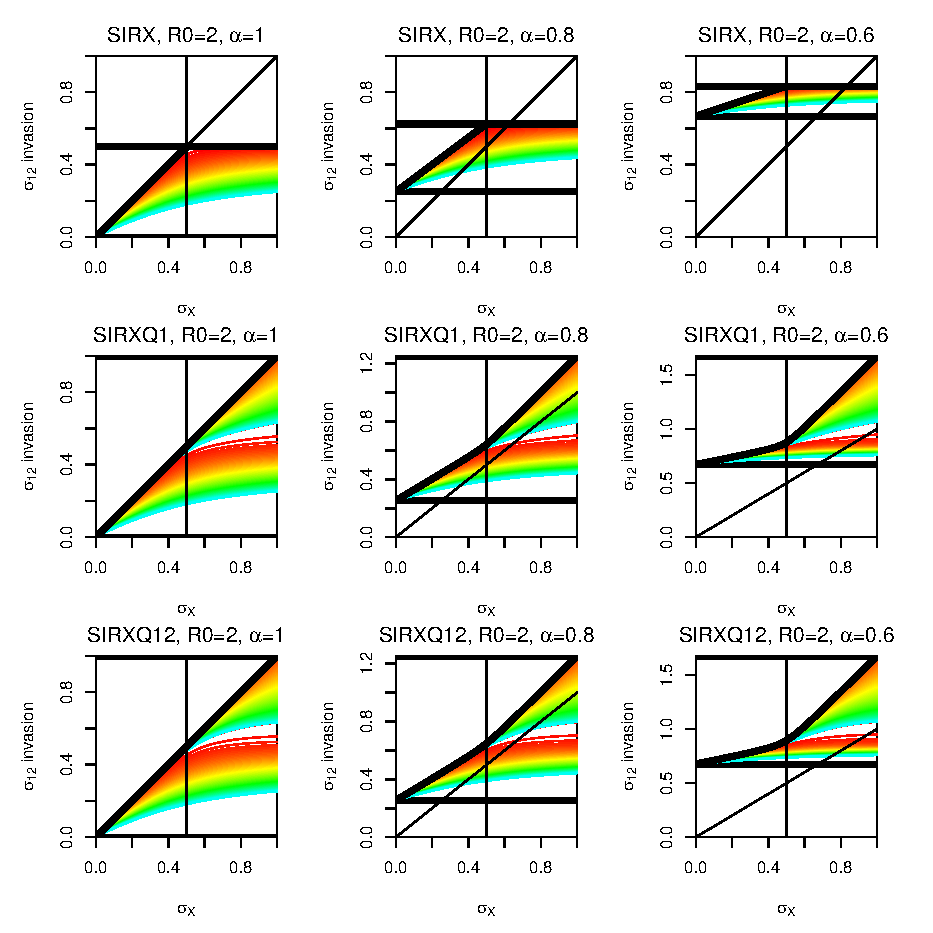
\includegraphics[width=0.8\linewidth]{texte/article3/graph/thresholdn1x_alpha_r02.eps}
  \caption{Invasion threshold. The y-axis represent the minimum
    $\sigma_{12}$ value needed to ensure that the IAU mutant can
    invade a population where a resident IAU is at the endemic
    equilibrium. Columns of figure indicate the effect of functional
    constraint ($\alpha$). Lines of figure present different versions
    of the $SIRX$ model. First line figures: without temporary full
    cross immunity ($Q$) ; second line figures: with $Q$ of duration
    $1/q=6$ months and without immune boosting ($Q1$) ; third line
    figures: with $Q$ ($1/q=6$ months) and immune boosting ($Q12$). In
    each figure, black curves represent the invasion threshold for the
    $SIR$ limit ($g=0$), the $SIRI$ limit ($g \to \infty$) and the
    $SIS$ limit ($g \to \infty$ ; $\sigma_{X}=1$) of the $SIRX$
    model. The $SIRS$ limit correspond to the value
    $\sigma_{X}=1$. Colours represent various values of $g$ from
    $1/g=1$ year (red) to $1/g=70$ years (blue) by 1 year. For second
    and third line figures, additional $1/g$ values are plotted with a
    second colour panel ranging from 0.01 (red) to 1 year (blue) by
    0.01 year.}
  \label{fig:threshold}
\end{figure}


When $\alpha=1$, invasion of the IAU mutant is always possible
whenever $\sigma_{12} > \sigma_{X}$. This sufficient condition (SC) is
not limited to our $SIRX$ model. As we show in the appendix, it
remains true in models allowing for a flexible shape for the evolution
of the reinfection probability within IAU due to gradual antigenic
drift such as the one used by \citet{Xia2005}. From a more biological
standpoint, this SC seems reasonable because it means that infection
by a given IAU confers a better protection against strains belonging
to the same IAU than against strains of another IAU. However, this SC
breaks down as functional constraints ($\alpha<1$) result in an
invasion threshold even when $\sigma_{12} > \sigma_{X}$
(Figure~\ref{fig:threshold}). In the following sections the SC is
always respected.




\section{Transient dynamics of the $SIRX$ model}

%Parameters values:

\subsection{Endemic equilibrium of the 1-IAU $SIRX$ model}

The endemic dynamics of the 1-IAU $SIRX$ model strongly depends on the
value of $g$ and $\sigma_{X}$. We have already shown that in the limit
$\sigma_{X}=1$ the $SIRX$ model is equivalent to the $SIRS$ model
whereas in the limit $g \to \infty$ it reduce to the $SIRI$ model of
\citep{Gomes2004a}. Unlike the $SIRS$ model, the $SIRI$ model presents
a phase transition with a sudden increase in the number of infectious
hosts near $\sigma_{X} = 1/R_0$ (defined as a reinfection threshold).
Figure~\ref{fig:eq_end} shows the evolution of the mean annual attack
rate (estimated on the order of 10\% for seasonal influenza
\citep{Cox2000a}) at the endemic equilibrium in function of $\sigma$
and $g$ for $R_{0}=2$ or 5.

\begin{figure}[!htbp]
  \center
  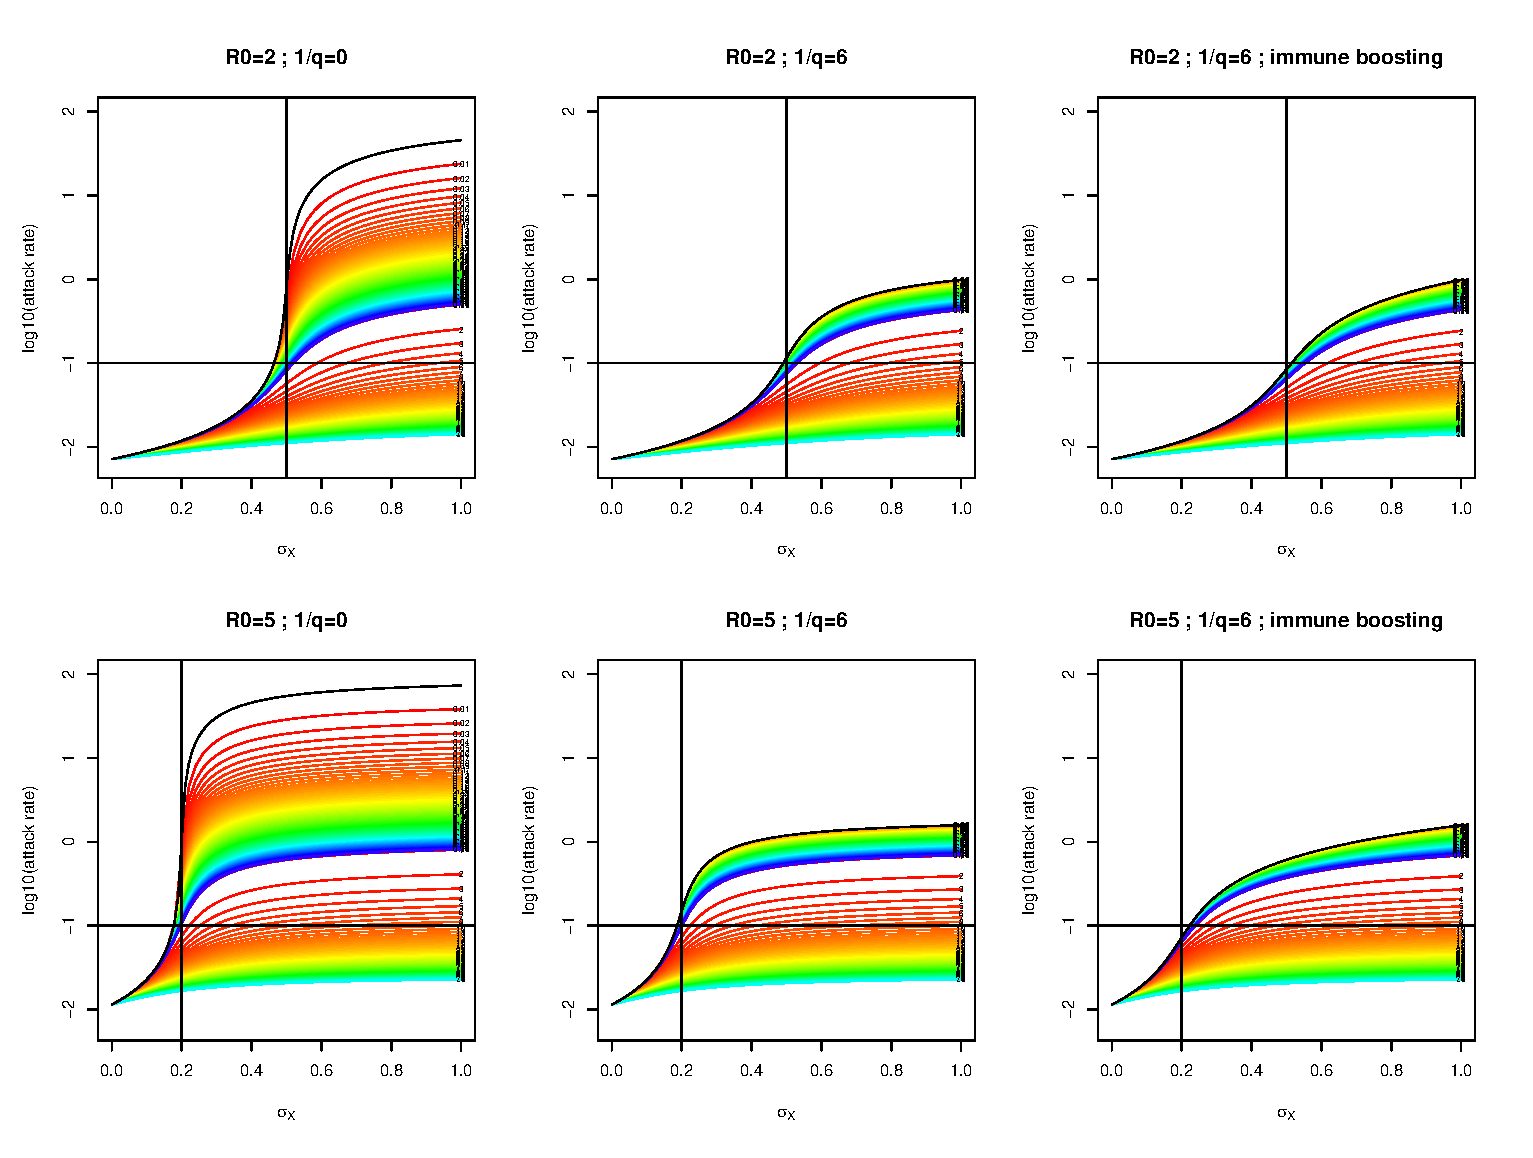
\includegraphics[width=0.7\linewidth]{texte/article3/graph/eq_end.eps}
  \caption{Evolution of the annual attack rate ($\frac{1}{N} \int_0^1
    \nu I(t) dt$) of a single antigenic unit at the endemic
    equilibrium of the $SIRX$ model (first column figures), the
    $SIRXQ1$ model ($1/q=6$ months) (second column figures) and the
    $SIRXQ12$ model ($1/q=6$ months) with immune boosting. Black line
    represent the reinfection limit of the model obtained as $g \to
    \infty$ ; Colours represent various values of $g$. First colour
    panel: $1/g$ varies from 0.01 year (red) to 1 years (blue) by 0.01
    years; second colour panel $1/g$ varies from 1 year (red) to 70
    years (blue) by 1 year.}
  \label{fig:eq_end}
\end{figure}

\subsection{Invasion-replacement dynamics with the 2-IAU $SIRX$ model}
\label{sec:replacement}
We consider the outcome of the invasion of a mutant IAU (indexed by 2)
within a population where a resident IAU (indexed by 1) is at the
endemic equilibrium previously described. Parameter values are the
same for both IAUs and no functional constraints are imposed to the
mutant ($\alpha=1$). Unlike the invasion condition, the outcome of the
invasion depends on the chosen function $f$ for the cross-protection
between IAU. For simplicity we do not assume cumulative effect of the
infection history and we choose the intuitive maximum cross-protection
function $\sigma_{Hk}=\min_{i\in H}\sigma_{ik}$ (see section
\ref{sec:seqeff} for further details). Since the SC is respected it
leads to $\sigma_{Hk}=\sigma_{X}$ when $H=\{1,2\}$ and $k\in\{1,2\}$.
The possible outcomes following invasion are: i) the resident only
goes extinct and it is replaced by the mutant (successful
replacement), ii) the mutant goes extinct and the resident maintains
(failed replacement), iii) both mutant and resident maintain
(coexistence), iv) both mutant and resident go extinct. Since we use
deterministic simulations we fix the extinction threshold at
$10^{-9}$. Figure~\ref{fig:sirx_area} illustrates these different
outcomes for all possible values of $\sigma_{X}$ and $\sigma_{12}$ and
for several values of $R_{0}$ and $g$. Note that for clarity, the
parameter space where the SC is not respected is also represented
($\sigma_{X}>\sigma_{12}$) and then exhibits the invasion threshold
found in section \ref{sec:invasion}.

% As we have already shown, the
%invasion can be prevented when partial protection to the previously
%encountered resident antigenic unit is higher than partial protection
%to a related new antigenic unit ($\sigma > \sigma_x$).  If there is
%not enough evidence to completely discard this case, we think that it
%lacks empirical and intuitive support and will mostly neglect it in
%the following.  We will therefore use the following susceptibility
%reduction the matrix: $\mathbf{M} = \bordermatrix{ & 1 & 2\cr 1 &
%  \sigma & \sigma_x \cr 2 & \sigma_x & \sigma \cr 12 & \sigma & \sigma
%  \cr }$ where $\sigma_x>\sigma$.

\begin{figure}[!htbp]
  \center
  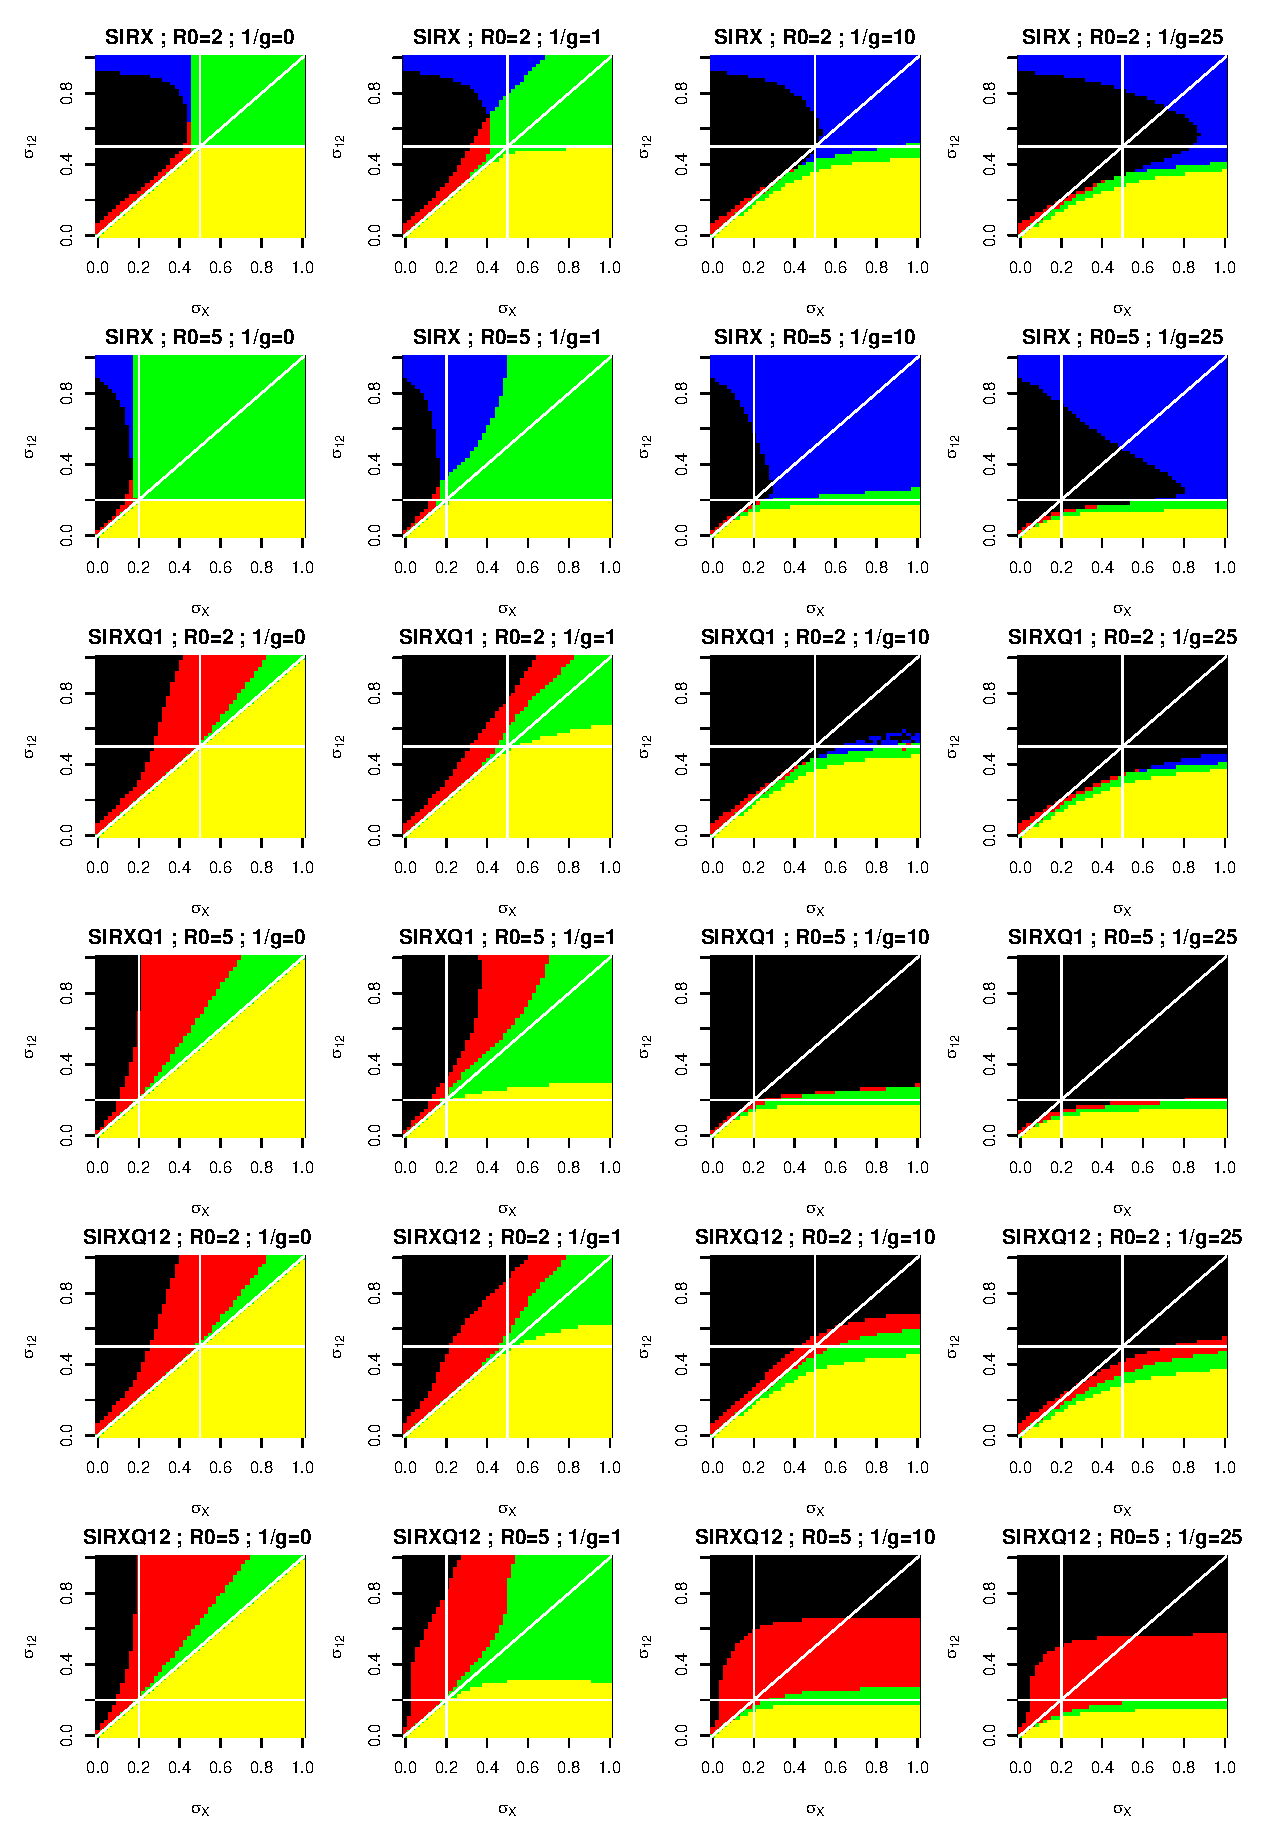
\includegraphics[width=0.8\linewidth]{texte/article3/graph/sens.eps}
  \caption{Outcomes of the transient invasion dynamics described in section \ref{sec:replacement} for the $SIRX$ (first and second line figures), the
    $SIRXQ1$ model ($1/q=6$ months) (third and fourth line figures) and the
    $SIRXQ12$ model ($1/q=6$ months) with immune boosting (fifth and
    sixth line figures). Colours: only the resident goes
    extinct (successful replacement, red), only the mutant goes
    extinct (blue); no IAU goes extinct (coexistence, green), both
    IAU go extinct (black), the
    mutant cannot invade (yellow). White lines indicate the reinfection
    threshold given by $1/R_{0}$.}
  \label{fig:sirx_area}
\end{figure}

Regarding the most interesting replacement area (RA, in red on figure
\ref{fig:sirx_area}) the first striking observation concerns its
smallness compared to other areas. The effects of the different
parameters on its size are the following: i) the RA is maximized when
the tempo of gradual antigenic drift is low ($1/g\thickapprox$ 1 year)
and it is almost nonexistent when $1/g>10$ years. ii) The RA is always
located below the reinfection threshold \textit{i.e.} when
$\sigma_{X}<1/R_{0}$ and consequently the RA decreases when $R_{0}$
increases. As $\sigma_{X} \to \frac{1}{R_0}$ coexistence is observed
instead of replacement. Indeed, since both IAUs benefit a greater
reinfection, the post epidemic extinction risk of the mutant is
reduced but in the same time this latter has less impact on the
resident which maintains (see also the appendix). iii) Finally, regarding the
effect of $\sigma_{12}$, the RA is only observed when the SC is
respected but we also note that the cross-protection within IAU must
not exceed by far the cross-protection between IAUs
($\sigma_{12}\gtrsim\sigma_{X}$). In other words, if we consider
$\Delta\sigma=|\sigma_{12}-\sigma_{X}|$ as a measure of the immune
escape of the mutant IAU over the resident IAU, then this immune
escape cannot exceed a few percents. Moreover, for a fixed value of
$\sigma_{X}<1/R_{0}$, the small RA indicates a high sensitivity to
$\sigma_{12}$ since a too great immune escape leads to the extinction
of both IAUs. This behaviour is confirmed in the appendix where it is
shown that despite the small RA the mutant IAU can produce attack rate
varying from 5 to 50 \%. This range encompasses attack rates observed
during antigenic cluster transition as well as during pandemic
antigenic shifts. Regarding the $SIRS$ limit of our $SIRX$ model (when
$\sigma_{X}=1$) we did not find any RA for any parameter value. On the
opposite, the $SIRI$ limit (when $g\to\infty$) exhibits the same RA
characteristics than the $SIRX$ model when $g>1\text{ }year^{-1}$.
These characteristics were previously reported by
\citet{Goekaydin2007} and this preliminary study on the $SIRX$ model
emphasizes the importance of the reinfection threshold for the
replacement of IAU.

In the following section we fix $R_0=2$ (as most of $R_0$ estimates
are within the range 1.5-2 \citep{Lessler2007}) and $1/g=1$ year
(found to generally maximise the RA) and we consider $\sigma_{X}$
values sufficiently high to ensure attack rates of the order of 10\%.
As revealed by figure~\ref{fig:eq_end} this last condition imposes to
take $\sigma_{X}$ smaller but close to the reinfection threshold. In
accord with \citet{Goekaydin2007}, we find that other values of $R_0$
in the range 1.5-5 do not alter the results provided that $\sigma_{X}$
is adapted to be smaller but close to $1/R_0$.


\subsection{Metapopulation dynamics and seasonality}

In order to study IAU replacement in a more realistic setting, we
incorporate the $SIRX$ model of eq~\eqref{eq:full} into a stochastic
metapopulation framework as depicted in
equation~\eqref{eq:full_metapop} where $\{c_l\}_{l\in\{1..L\}}$
denotes the set of the $L$ cities.

\begin{footnotesize}
  \begin{align}
    \label{eq:full_metapop}
    \dot{R_{c_l}}_{\begin{subarray}{l}\varnothing \\ \varnothing \end{subarray}} &= \mu_{c_l} N_{c_l} -\sum_k \beta_k(t) {R_{c_l}}_{\begin{subarray}{l}\varnothing \\ \varnothing \end{subarray}} \frac{I_{c_l}^k}{N_{c_l}} - \mu_{c_l} {R_{c_l}}_{\begin{subarray}{l}\varnothing \\ \varnothing \end{subarray}}\\
%%
    \dot{R_{c_l}}_{\begin{subarray}{l}H\\ J \end{subarray}} &= \sum_{k
      \in J} \beta_k \sigma_{Hk} {R_{c_l}}_{\begin{subarray}{l}H \\ J
        \setminus k \end{subarray}} \frac{I_{c_l}^k}{N_{c_l}} -\sum_{k
      \notin J} \beta_k(t) \sigma_{Hk}
    {R_{c_l}}_{\begin{subarray}{l}H\\ J \end{subarray}}
    \frac{I_{c_l}^k}{N_{c_l}} - \sum_{k \in J} g_k
    {R_{c_l}}_{\begin{subarray}{l}H\\ J \end{subarray}} + \sum_{k \in
      \{H \setminus J\}} g_k {R_{c_l}}_{\begin{subarray}{l}H\\ J\cup
        k \end{subarray}} -\mu_{c_l}
    {R_{c_l}}_{\begin{subarray}{l}H\\J \end{subarray}} \notag \\
%%
    \dot{I_{c_l}}^k &= \sum_{\begin{subarray}{l}H \subseteq \mathbf{K}
        \\ J \subseteq \{H \setminus k \} \end{subarray}}
    {R_{c_l}}_{\begin{subarray}{l}H \\ J \end{subarray}}
    \frac{I_{c_l}^k}{N_{c_l}} -\nu I_{c_l}^k -\mu_{c_l} I_{c_l}^k
    -\sum_{m\neq l} \frac{\tau_{c_lc_m}}{N_{c_l}} I_{c_l}^k
    +\sum_{m\neq l} \frac{\tau_{c_mc_l}}{N_{c_l}} I_{c_m}^k \notag
  \end{align}
\end{footnotesize}

For simplicity, only infectious hosts are allowed to travel,
$\frac{\tau_{c_mc_l}}{N_{c_l}}$ being the probability that a host
located in city $c_l$ of size $N_{c_l}$ travels to city $c_m$.
Eq~\eqref{eq:full_metapop} was simulated on a network of 52 global
cities (depicted in the appendix) linked by air transportation data
from year 2000 and published in \citep{Grais2003}. Population sizes of
each city were taken from http://unstats.un.org/unsd/demographic/.
Seasonal forcing was introduced for cities in temperate areas with a
sinusoidal varying transmission rate $\beta(t)= \frac{1}{2} \left[
  (1-\frac{\beta_{min}}{\beta_{max}}) \sin(2 \pi
  \frac{(t-t_{max})}{365}+\frac{\pi}{2}) +1
  +\frac{\beta_{min}}{\beta_{max}} \right]$ with phase opposition for
North and South hemisphere (\citep{Finkelman2007}). No seasonal
forcing was assumed in the tropics as transmission appears to be more
constant \citep{Viboud2006}.

\subsubsection{Invasion-replacement in the stochastic metapopulation model}

We applied a similar invasion protocol as in the deterministic
framework of section \ref{sec:replacement}.
Figure~\ref{fig:sirx_s03_039} (see also the appendix.) reveals that
simulations of the stochastic metapopulation model are in good
agreement with the previously studied deterministic model. Indeed, the
RA is maximised when $\sigma_{X}$ is close to $1/R_0$. Moreover, as
$\sigma_{X}$ approaches $1/R_0$, coexistence substitutes replacement
and higher values of $\sigma_{12}$ are needed to ensure the resident
IAU replacement by the mutant one.

The appendix reveal that we also find a high sensitivity to the immune
escape $\Delta\sigma$ of the mutant. $\Delta\sigma\approx2\%-3\%$ are
sufficient to ensure successful antigenic unit replacement whereas
higher values result in unrealistic high epidemics (within a few
percent of immune escape the ratio of the maximum epidemic size of the
mutant over the resident was found to vary from 1 to 100) .

\begin{figure}[htp]
  \center
  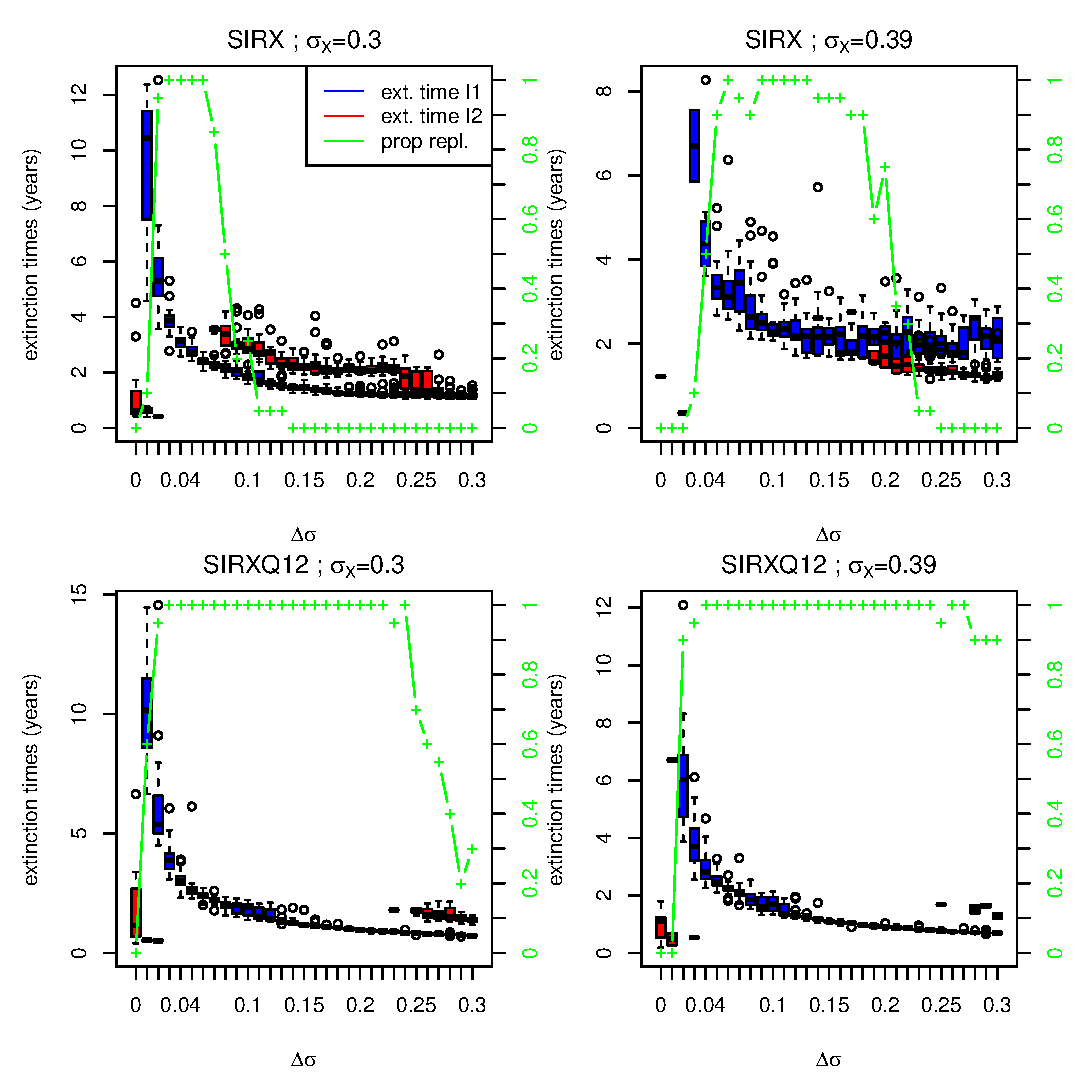
\includegraphics[width=0.7\linewidth]{texte/article3/graph/sirx_s03_039_final.eps}
  \caption{Replacement area (RA) for 20 realisations of the stochastic
    $SIRX$ model (first line figures) and $SIRXQ12$ with immune boosting (second line)
    metapopulation model . The mutant antigenic unit (red) is
    introduced in april 1$^{st}$ in Shenzen.  Parameters: $R_0=2$; $1/\nu=4$ days ; $1/g=1$
    year; $\sigma_{X}=0.3$
    (top) or $\sigma_{X}=0.39$ (bottom, chosen to maximize the RA). No seasonal forcing is assumed in the tropics and northern
    and southern hemisphere are forced with phase opposition
    ($t^{north}_{max}= 356$, $t^{south}_{max}= 173$) with intensity
    $\frac{\beta_{min}}{\beta_{max}}=0.4$.}
  \label{fig:sirx_s03_039}
\end{figure}


\subsubsection{Sequential effect}
\label{sec:seqeff}
We extend the previous analysis by considering the successive emergence of
IAUs. When three or more IAUs are co-circulating it is
necessary to specify the general function $f$ that defines the cross-protection conferred by previous IAU exposures against infection by new IAUs. As stated by \citet{Adams2007a}, very
little empirical information relating to the shape of $f$ is available and most
previous models have used either a minimum or a multiplicative function.  The
minimum function assumes that only antibodies to the most related IAU of the host immune repertoire are produced. The multiplicative function assumes
that antibodies of the entire host immune repertoire are produced and their net
benefit is greater than either one of them alone. In reality, host immune response should lie between these two extrema. However, as the minimum
function is the most extensively used by previous models and in the absence
of any strong evidence for an alternative function, we choose to use it in
this study.

The cross-protection factor $\sigma_{Hk}$ is thus the same as the one previously described in section \ref{sec:replacement}: $\sigma_{Hk}=\min_{i\in H}\sigma_{ik}$ and since all IAUs have the same reinfection parameter $\sigma_{Hk}=\sigma_{X}$ if $k\in H$.

The specific cross-protection factor $\sigma_{ik}$ encapsulates the
evolution of antigenic distance between two IAUs where $i$ and $k$
refer to the order of emergence of both IAUs. Various forms can be
chosen to describe this evolution but they are not without strong
consequences \citep{Adams2007a}. As a simple starting point, we will
consider a linear function by assuming that $\sigma_{ik} = \sigma_{X}
+ \Delta\sigma |k-i|$ where $|k-i|$ is the kinship level between IAU
$i$ and IAU $k$. In agreement with experimental studies on influenza
A/H3N2 antigenic clusters (\citet{Smith2004}), IAUs are sequentially
introduced every 4 years in Shenzen on april $1^{st}$ with an initial
seed of 100 infected hosts to prevent stochastic extinctions at the
beginning of the invasion.

Simulations of the 5-IAUs $SIRX$ stochastic metapopulation model
confirm the high sensitivity of the model to $\Delta\sigma$. Immune
escapes greater than 5\% lead to unrealistic high epidemics as well as
too long refractory periods compared to data
(figure~\ref{fig:world_sirx} illustrates the effect of an increasing
sequence of $\Delta\sigma$). As shown in the appendix, simulations
where $\sigma_{X} \to \frac{1}{R_0}$ exhibit long periods of
coexistence with old IAUs being maintained at low incidence.

\begin{figure}[!htbp]
  \center
  \includegraphics[width=0.8\linewidth]{texte/article3/graph/traj_metapop.eps}
  \caption{Typical realisation of the $SIRX$ model (top panel) and
    $SIRXQ12$ model (bottom panel) with immune boosting in the
    stochastic metapopulation framework in the city of Paris. First
    IAU is at the endemic equilibrium and 4 other IAUs are
    sequentially introduced every 4 years in Shenzen on april 1$^{st}$
    with an initial seed of 100 infected hosts. y-axis is weekly
    incidence per 100 000 inhabitants. Parameters: $\sigma_{X}=0.3$
    and $\Delta\sigma\in\{0.01, 0.02, 0.05, 0.1\}$. Other parameters
    are identical to figure~\ref{fig:sirx_s03_039}. Vertical plain
    (dotted) lines correspond to the introduction (worldwide
    extinction) times of the IAUs coded by colours. Corresponding
    annual attack rates are plotted in the appendix.}
  \label{fig:world_sirx}
\end{figure}

In summary, realistic antigenic cluster replacement with the $SIRX$
model appears possible only for a small range of cross-immunity
parameters ($\sigma_{X}$ and $\Delta\sigma$). We have seen that to
ensure recurrent epidemics with attack rates comparable to data, the
reinfection parameter of each IAU ($\sigma_{X}$) must be smaller but
close to $1/R_0$. Furthermore, for a fixed value of $\sigma_{X}$, the
epidemic size of a newly introduced IAU is highly sensitive to its
immune escape since $\Delta\sigma>5\%$ results in unrealistic high
epidemic size followed by too long refractory periods. On the other
hand, when $\Delta\sigma< 5 \%$ our $SIRX$ model is able to reproduce
the patterns observed in real data. Recently, \citet{Finkenstaedt2005}
have obtained similar estimates of immune escape intensity in a study
using french influenza-like illness data as well as a model allowing
for both gradual and punctuated renewal of susceptible. Despite
conceptual differences between our two models, their punctuated immune
escape estimates can be related to our $\Delta\sigma$ parameter. Their
results show that punctuated immune escape are all smaller than 7\%
with 53\% of the estimates $\leq 2\%$, 26.7\% between 2 and 5 \% and
20\% between 5 and 7 \%, which is in accordance with the values needed
by the $SIRX$ model. However, \citet{Finkenstaedt2005} found 15
discrete antigenic jumps between the years 1985 and 2002, a pattern
more related to noisy gradual antigenic drift than to rarer antigenic
cluster transitions (on average, clusters remained dominant for 3.3
years \citep{Smith2004}).

From our side, the small amount of immune escape between IAUs when
compared with the high amount of reinfection within IAU ($\Delta\sigma
<< \sigma_{X}$) seems not in agreement with previous studies on
cross-protection and influenza A/H3N2 antigenic clusters. In 2004,
\citeauthor{Smith2004} have presented a 2D antigenic map of 273 viral
isolates of human influenza A/H3N2. Their study reveals that strains
tend to group in clusters rather than to form a continuous antigenic
lineage. Since cross-immunity is closely related to antigenic
distance, it is expected that cross-immunity within clusters is much
higher than cross-immunity between clusters. For instance
\citet{Koelle2009} considered a 60-80 \% degree of cross-immunity
between successive antigenic clusters and a full cross-immunity
between strains belonging to the same cluster. With our notations, it
amounts to considering $\sigma_{X}=0$ and
$\sigma_{ij}=\sigma_{X}+\Delta\sigma|i-j|=\Delta\sigma=20-40\%$ where
$i$ and $j$ are two successive IAUs. Figure \ref{fig:sirx_area}
reveals that within this parameter range IAU replacement is impossible
and complete extinction of both IAUs is observed (see also the
appendix). 

A more detailed discussion on the scale of $\Delta$ can be found in
the discussion. In the next sections, we introduce factors that
increase the range of immune escape leading to successful IAU
replacement.


\subsection{Functional constraints and evolutionary trade-off between
  immune escape and transmission}

There is large evidence for functional constraints and evolutionary
trade-off associated with IAU transitions \citep{Rambaut2008}.
Figure~\ref{fig:threshold} reveals that $\alpha<1$ impairs invasion of
a mutant IAU even if $\sigma_{12}>\sigma_{X}$. Functional constraints
can then result in higher values for $\Delta\sigma$ but it
nevertheless remains to test to what extent a resident IAU can be
replaced by an intrinsically less fit IAU mutant. The situation is all
the more complicated to model as compensatory mutations are expected
in nature. We address the question in a simple way by only examining
the mutant invasion, assuming that the $\alpha$ parameter remains
constant during the initial outbreak.

\begin{figure}[!htbp]
  \center
  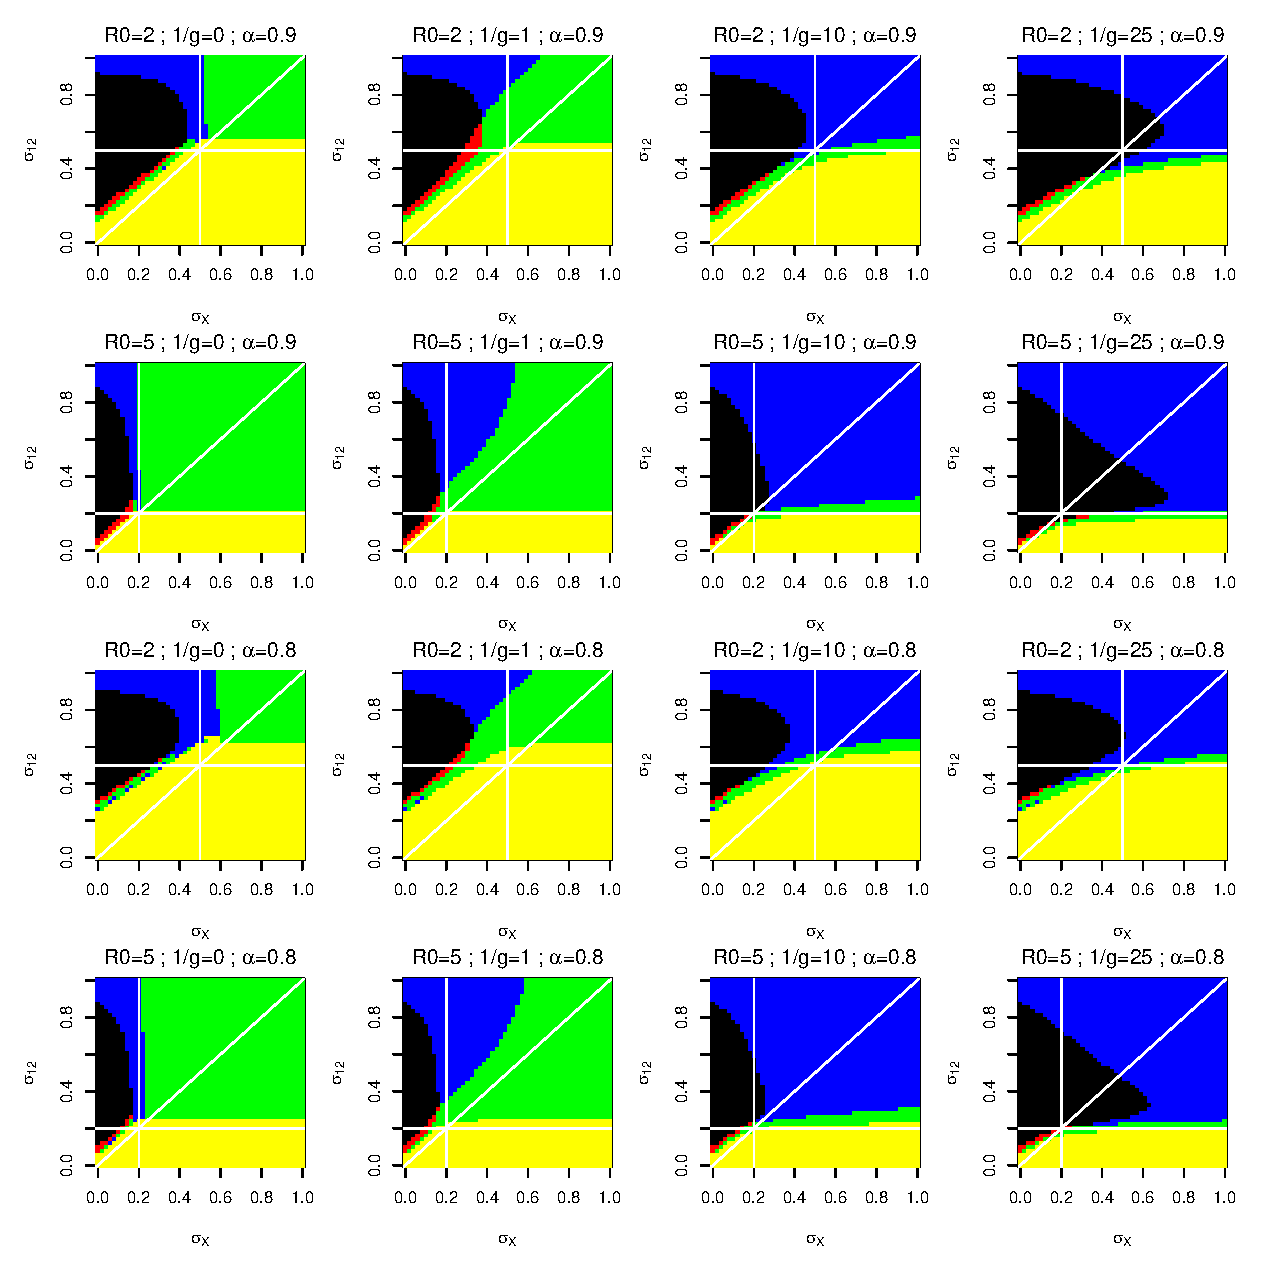
\includegraphics[width=0.8\linewidth]{texte/article3/graph/sirx_trade_off_short.eps}
  \caption{Effect of functional constraints ($\alpha\in\{0.9,0.8\}$)
    on the invasion outcome of a mutant IAU within a population where
    a resident IAU is at the endemic equilibrium for the $SIRX$ model.
    Color legend is identical as figure~\ref{fig:sirx_area}}
  \label{fig:sirx_trade_off_09}
\end{figure}

Figure~\ref{fig:sirx_trade_off_09} (see also the appendix) reveal that
the functional constraints translate the RA into greater
$\Delta\sigma$ values and allow higher antigenic distance between
successive IAUs. In the other hand, the RA is significantly narrow
comparing to figure \ref{fig:sirx_area} and new coexistence areas are
observed. Given the existing variability observed in immune escape
intensity such a situation can result in alternate periods of
coexistence and replacement. However, the full study of this pattern
will require a way to model compensatory mutations which is beyond the
scope of this paper.


\section{Temporary period of IAU-transcending immunity}


\subsection{Biological hypothesis}
\label{sec:Q}

The existence of a period of temporary full protection against infection by any strain was
originally proposed by \citet{Webster1992} to explain subtype
replacement during pandemics \textit{i.e.} when partial
cross-protection ensured by anti-HA and NA antibodies is low.
\citet{Webster1992} suggested that such full protection
could be mediated by CD8+ T-lymphocyte response to the shared internal
proteins among human influenza A virus.

\citet{Webster1992} prediction was confirmed by \citet{Ferguson2003}
who also revealed that this period was of tremendous importance to
restrict strain diversity during seasonal influenza in absence of
antigenic clusters. These results were analysed by \citet{Tria2005}
who argued that temporary strain-transcending immunity could only
restrict strain diversity if it was coupled with a source of
heterogeneity. One important difference between \citet{Ferguson2003}
and \citet{Tria2005} individual based model was the way this period
was introduced. In \citet{Ferguson2003} study, following exposure to a
strain $s$ (due to a close contact with an infectious host) the
probability of becoming infected depends on the strain $s$ and the
host's immune repertoire $H$. But whatever the outcome of the
exposure, the host acquires a short-lived strain-transcending immunity
that we can mechanistically represent by a new class $Q$ of expected
duration $1/q=6$ months. However, for a better understanding of what
is ``doing'' the $Q$ class we must detail the three ways a host enters
it following exposure:
\begin{enumerate}
\item if $s\notin H$ and $H$ fails to confer sufficient
  cross-protection, the host becomes infected, updates $H\rightarrow
  H\cup\{s\}$ and enters the $Q$ class (case $Q_{1}$)
\item if $s\notin H$ and $H$ confers sufficient cross-protection, the
  host escapes infection he does not updates $H$ and enters the $Q$
  class (case $Q_{2}$)
\item if $s\in H$ the host escapes infection and enters the $Q$ class
  (case $Q_{3}$)
\end{enumerate}

The biological justification of $Q_{1}$ implies triggering of cellular
immunity following infection, a process confirmed in various animals
models \citep{Grebe2008} whereas $Q_{2}$ and $Q_{3}$ refer to the
immune boosting assumption \citep{Ferguson2003}. This interpretation
is discussed further in the discussion. By contrast,
\citet{Tria2005} implemented only the case $Q_{1}$. As we show in
the following, this could be responsible for the differing conclusions
between the two models.

Figure \ref{Q123} illustrates the three assumptions on the $Q$ class
in the context of IAU instead of strains as used in this paper.

\begin{figure}[htbp]
\begin{center}
\begin{tikzpicture}[node distance=3cm, auto,>=latex', thick]
  \tikzstyle{sebQ3}=[rectangle, fill=red, draw=gray, text=black]
  \tikzstyle{sebQ}=[rectangle, fill=red!20, draw=gray, text=black]
  \tikzstyle{seb}=[rectangle, fill=blue!20, draw=gray, text=black]
  \node [seb] (X_1_1) {$R_{\begin{subarray}{l}H \\ J\end{subarray}}$};
  \node [seb, right of=X_1_1,node distance=3cm] (I_2_1_1) {$I^{k}_{\begin{subarray}{l}H \\J\end{subarray}}$};
  \node [sebQ, right of=I_2_1_1,node distance=2cm] (Q_12_12) {${Q_1}_{\begin{subarray}{l}H(\cup k) \\J\cup k\end{subarray}}$};
  \node [sebQ, below of=X_1_1,node distance=2cm] (Q2_1_1) {${Q_2}_{\begin{subarray}{l}H \\J\end{subarray}}$};
  \node [sebQ3, above of=X_1_1,node distance=2cm] (Q3_1_1) {${Q_3}_{\begin{subarray}{l}H \\J\end{subarray}}$};
  \node [seb, right of=Q_12_12,node distance=2cm] (X_12_12) {$R_{\begin{subarray}{l}H(\cup k) \\J\cup k\end{subarray}}$};
  
  \draw [->] (X_1_1) --node {$\beta \sigma^k_{H} I^{k:k \notin J}$} (I_2_1_1);
  \draw [->] (X_1_1) edge[bend right]node[left] {$\beta (1-\sigma^k_{H})I^{k:k \notin J}$} (Q2_1_1);
  \draw [->] (Q2_1_1) edge[bend right]node[right] {$q$} (X_1_1);
  
  \draw [->] (X_1_1) edge[bend left]node[left] {$\beta  I^{k:k \in J}$} (Q3_1_1);
  \draw [->] (Q3_1_1) edge[bend left]node[right] {$q$} (X_1_1);
  
  \draw [->] (I_2_1_1) --node{$\nu$}(Q_12_12);
  \draw [->] (Q_12_12) --node{$q$}(X_12_12);
\end{tikzpicture}
\caption{Three mechanisms for the temporary period of IAU-transcending
  immunity (red boxes). When exposed to an IAU $k$ that does not
  belong to the effective immune repertory $J$ ($k \notin J$) , hosts
  enter $Q_{1}$ after infection whereas they enter $Q_{2}$ if their
  immune history $H$ succeed in conferring immunity against $k$ (and
  therefore avoid the infection). Hosts protected to $k$ due to
  effective immunity ($k \in J$) always escape infection but
  nevertheless enter $Q_{3}$ after an exposure.}
\label{Q123}
\end{center}
\end{figure}

\clearpage




\subsection{Extension of the simple $SIRX$ model}

Eq. \eqref{eq:fullQ} extends eq. \ref{eq:full} to incorporate the
assumption of temporary IAU-transcending immunity under case $Q_{1}$.
Note also that co-infection is not allowed anymore. This model is
labeled $SIRXQ_{1}$.

\begin{footnotesize}
  \begin{align}
    \label{eq:fullQ}
    \dot{R}_{\begin{subarray}{l}\varnothing \\
        \varnothing \end{subarray}} &= \mu N -\sum_k \beta_k(t) R_{\begin{subarray}{l}\varnothing \\ \varnothing \end{subarray}} \frac{I^k}{N} - \mu R_{\begin{subarray}{l}\varnothing \\ \varnothing \end{subarray}}\\
  %% 
    \dot{I}^k_{\begin{subarray}{l}H\\ J \setminus k \end{subarray}} &=
    \beta_k(t) \sigma_{Hk} R_{\begin{subarray}{l}H \\ J\setminus
        k \end{subarray}} \frac{I^k}{N} -\nu I^k_{\begin{subarray}{l}H
        \\ J \setminus k \end{subarray}} -\sum_{m \in J \setminus k}
    g_m I^k_{\begin{subarray}{l}H \\ J \setminus k \end{subarray}} +
    \sum_{m \in (H \setminus (J \cup k))} g_m
    I^k_{\begin{subarray}{l}H \\ (J \setminus k) \cup
        m \end{subarray}}
    -\mu I^k_{\begin{subarray}{l}H \\ J \setminus k \end{subarray}} \notag \\
  %% 
    \dot{Q}_{\begin{subarray}{l}H\\ J \end{subarray}} &= \sum_{k \in
      J} \nu I^k_{\begin{subarray}{l}H \setminus k \\ J \setminus
        k \end{subarray}} +\sum_{k \in J} \nu
    I^k_{\begin{subarray}{l}H \\ J \setminus k \end{subarray}} -q
    Q_{\begin{subarray}{l}H \\ J\end{subarray}} -\sum_{m \in J} g_m
    Q_{\begin{subarray}{l}H \\ J\end{subarray}} + \sum_{m \in (H
      \setminus J )} g_m Q_{\begin{subarray}{l}H \\ J \cup
        m \end{subarray}} -\mu
    Q_{\begin{subarray}{l}H \\ J \end{subarray}} \notag \\
  %% 
    \dot{R}_{\begin{subarray}{l}H\\ J \end{subarray}} &= q
    Q_{\begin{subarray}{l}H \\ J\end{subarray}} -\sum_{k \notin J}
    \beta_k(t) \sigma_{Hk} R_{\begin{subarray}{l}H\\ J \end{subarray}}
    \frac{I^k}{N} - \sum_{m \in J} g_m R_{\begin{subarray}{l}H\\
        J \end{subarray}} + \sum_{m \in (H \setminus J)} g_m
    R_{\begin{subarray}{l}H\\ J\cup m \end{subarray}} -\mu
    R_{\begin{subarray}{l}H\\J \end{subarray}} \notag
  \end{align}
\end{footnotesize}


where $$I^k=\sum_{\begin{subarray}{l}H \subseteq \mathbf{K} \\ J
    \subseteq H \end{subarray}} I^k_{\begin{subarray}{l}H\\ J
    \setminus k \end{subarray}}$$.

and the number of equations is given by: $$2 \sum_{k=0}^{N_K} \left
  (\binom{N_K}{k} \sum_{p=0}^k \binom {k}{p} \right) + \sum_{k=0}^{N_K}
\left( \binom{N_K}{k} \sum_{p=0}^k \binom{k}{p}(N_K-p) \right ) $$

In order to investigate the additional effect of assumption $Q_{2}$ we
modify eq \eqref{eq:fullQ} and obtain eq \eqref{eq:fullQferg}. The
corresponding model is labeled $SIRXQ_{12}$.

\begin{footnotesize}
  \begin{align}
    \label{eq:fullQferg}
    \dot{R}_{\begin{subarray}{l}\varnothing \\
        \varnothing \end{subarray}} &= \mu N -\sum_k \beta_k(t) R_{\begin{subarray}{l}\varnothing \\ \varnothing \end{subarray}} \frac{I^k}{N} - \mu R_{\begin{subarray}{l}\varnothing \\ \varnothing \end{subarray}}\\
%%
    \dot{I}^k_{\begin{subarray}{l}H\\ J \setminus k \end{subarray}} &=
    \beta_k(t) \sigma_{Hk} R_{\begin{subarray}{l}H \\ J\setminus
        k \end{subarray}} \frac{I^k}{N} -\nu I^k_{\begin{subarray}{l}H
        \\ J \setminus k \end{subarray}} -\sum_{m \in J \setminus k}
    g_m I^k_{\begin{subarray}{l}H \\ J \setminus k \end{subarray}} +
    \sum_{m \in (H \setminus (J \cup k))} g_m
    I^k_{\begin{subarray}{l}H \\ (J \setminus k) \cup
        m \end{subarray}}
    -\mu I^k_{\begin{subarray}{l}H \\ J \setminus k \end{subarray}} \notag \\
%%
    \dot{Q}_{\begin{subarray}{l}H\\ J \end{subarray}} &= \sum_{k \in
      J} \nu I^k_{\begin{subarray}{l}H \setminus k \\ J \setminus
        k \end{subarray}} +\sum_{k \in J} \nu I^k_{\begin{subarray}{l}H \\
        J \setminus k \end{subarray}} -q Q_{\begin{subarray}{l}H \\ J
      \end{subarray}} -\sum_{m \in J } g_m Q_{\begin{subarray}{l}H \\
        J \end{subarray}} + \sum_{m \in (H \setminus J)} g_m
    Q_{\begin{subarray}{l}H \\ J \cup m \end{subarray}} -\mu
    Q_{\begin{subarray}{l}H \\ J \end{subarray}} \notag \\
%%
    \dot{Q'}_{\begin{subarray}{l}H\\ J \end{subarray}} &= \sum_{k
      \notin J} -\beta_k(t) (1 -\sigma_{Hk}) R_{\begin{subarray}{l}H\\
        J \end{subarray}} \frac{I^k}{N} -q Q'_{\begin{subarray}{l}H \\
        J \end{subarray}} -\sum_{m \in J} g_m Q'_{\begin{subarray}{l}H
        \\ J \end{subarray}} + \sum_{m \in (H \setminus J)} g_m
    Q'_{\begin{subarray}{l}H \\ J \cup m \end{subarray}} -\mu
    Q'_{\begin{subarray}{l}H \\ J \end{subarray}} \notag \\
%%
    \dot{R}_{\begin{subarray}{l}H\\ J \end{subarray}} &= q
    Q_{\begin{subarray}{l}H \\ J \end{subarray}} +q
    Q'_{\begin{subarray}{l}H \\ J \end{subarray}} +\sum_{k \notin J}
    -\beta_k(t) R_{\begin{subarray}{l}H\\ J \end{subarray}}
    \frac{I^k}{N} - \sum_{m \in J} g_m R_{\begin{subarray}{l}H\\
        J \end{subarray}} + \sum_{m \in (H \setminus J)} g_m
    R_{\begin{subarray}{l}H\\ J\cup m \end{subarray}} -\mu
    R_{\begin{subarray}{l}H\\J \end{subarray}} \notag
  \end{align}
\end{footnotesize}

As in the $SIRX$ model, the reinfection limit of eq \eqref{eq:fullQ}
($SIRIQ_{1}$) and eq \eqref{eq:fullQferg} ($SIRIQ_{12}$) is obtained
as $g \to \infty$ (see the appendix).

\begin{footnotesize}
  \begin{align}
    \label{eq:fullQferg}
    \dot{R}_{\begin{subarray}{l}\varnothing \\
        \varnothing \end{subarray}} &= \mu N -\sum_k \beta_k(t) R_{\begin{subarray}{l}\varnothing \\ \varnothing \end{subarray}} \frac{I^k}{N} - \mu R_{\begin{subarray}{l}\varnothing \\ \varnothing \end{subarray}}\\
%%
    \dot{I}^k_{\begin{subarray}{l}H\\ J \setminus k \end{subarray}} &=
    \beta_k(t) \sigma^k_{H} R_{\begin{subarray}{l}H \\ J\setminus
        k \end{subarray}} \frac{I^k}{N} -\nu I^k_{\begin{subarray}{l}H
        \\ J \setminus k \end{subarray}} -\sum_{m \in J \setminus k}
    g_m I^k_{\begin{subarray}{l}H \\ J \setminus k \end{subarray}} +
    \sum_{m \in H \setminus (J \cup k)} g_m
    I^k_{\begin{subarray}{l}H \\ (J \setminus k) \cup
        m \end{subarray}}
    -\mu I^k_{\begin{subarray}{l}H \\ J \setminus k \end{subarray}} \notag \\
%%
    \dot{{Q_1}}_{\begin{subarray}{l}H\\ J \end{subarray}} &= \sum_{k \in
      J} \nu I^k_{\begin{subarray}{l}H \setminus k \\ J \setminus
        k \end{subarray}} +\sum_{k \in J} \nu I^k_{\begin{subarray}{l}H \\
        J \setminus k \end{subarray}} -q {Q_1}_{\begin{subarray}{l}H \\ J
      \end{subarray}} -\sum_{m \in J } g_m {Q_1}_{\begin{subarray}{l}H \\
        J \end{subarray}} + \sum_{m \in H \setminus J} g_m
    {Q_1}_{\begin{subarray}{l}H \\ J \cup m \end{subarray}} -\mu
    {Q_1}_{\begin{subarray}{l}H \\ J \end{subarray}} \notag \\
%%
    \dot{{Q_2}}_{\begin{subarray}{l}H\\ J \end{subarray}} &= \sum_{k
      \in K\setminus J} -\beta_k(t) (1 -\sigma^k_{H}) R_{\begin{subarray}{l}H\\
        J \end{subarray}} \frac{I^k}{N} -q {Q_2}_{\begin{subarray}{l}H \\
        J \end{subarray}} -\sum_{m \in J} g_m {Q_2}_{\begin{subarray}{l}H
        \\ J \end{subarray}} + \sum_{m \in H \setminus J} g_m
    {Q_2}_{\begin{subarray}{l}H \\ J \cup m \end{subarray}} -\mu
    {Q_2}_{\begin{subarray}{l}H \\ J \end{subarray}} \notag \\
%%
    \dot{R}_{\begin{subarray}{l}H\\ J \end{subarray}} &= q
    {Q_{1}}_{\begin{subarray}{l}H \\ J \end{subarray}} +q
    {Q_2}_{\begin{subarray}{l}H \\ J \end{subarray}} +\sum_{k \in K\setminus J}
    -\beta_k(t) R_{\begin{subarray}{l}H\\ J \end{subarray}}
    \frac{I^k}{N} - \sum_{m \in J} g_m R_{\begin{subarray}{l}H\\
        J \end{subarray}} + \sum_{m \in H \setminus J} g_m
    R_{\begin{subarray}{l}H\\ J\cup m \end{subarray}} -\mu
    R_{\begin{subarray}{l}H\\J \end{subarray}} \notag
  \end{align}
\end{footnotesize}


We did not however investigate the effects of the three cases
$Q_{123}$ together (see the discussion for a justification).
  
\subsection{Invasion threshold for the $SIRXQ_{1/12}$ model}

The general sufficient condition (SC) established in the appendix
still holds and ensures that invasion of a mutant IAU (with the same
basic reproduction number as the resident) whenever
$\sigma_{12}>\sigma_{X}$. Otherwise, the invasion threshold is given
by:
$$\sigma_{12} \geq \frac{1-r_2  R_{\begin{subarray}{l}\varnothing \\
      \varnothing \end{subarray}}^*}{r_2( R_{\begin{subarray}{l} 1 \\
      1 \end{subarray}}^* + R_{\begin{subarray}{l} 1 \\
      \varnothing \end{subarray}}^*)}$$ and show the large impact of
functional constraints. As illustrated in figure~\ref{fig:threshold}:
compared to the simple $SIRX$ model, $\sigma_{12}$ values greater than
one are needed to overcome the effects of functional constraints for
low $1/g$ values.

\subsection{Transient dynamics}

Figure~\ref{fig:sirx_area} (see also the appendix) illustrates the
effects of a 6 month period of temporary IAU-transcending immunity on
the invasion outcomes of a mutant IAU in a population where a resident
IAU is at the endemic equilibrium (see section \ref{sec:replacement}
for protocol details). As a general consequence of both $Q_{1}$ and
$Q_{2}$ classes is the significant increase of the $\Delta\sigma$
parameter range where IAU replacement occurs. This effect is achieved
by transforming coexistence area (green) of figure \ref{fig:sirx_area}
in replacement area (red) but also by enabling persistence of the
mutant for parameter range where the invasion would have resulted in
the extinction of both IAUs (black areas). This latter effect is
particularly present for the $SIRXQ_{12}$ model except close to the
reinfection limit where few effect of the $Q_{2}$ assumption can be
detected. As already noticed by \citet{Ferguson2003} immune boosting
($Q_{2}$) therefore acts as an important density dependent constraint
reducing incidence. This can be further confirmed in the appendix
where attack rates increase slower as a function of immune escape
$\Delta\sigma$ in the presence of immune boosting. As a last point,
the effects of the $Q_{1/2}$ classes increases with $R_{0}$
(Figure~\ref{fig:sirx_area}).
% Moreover with $R_0\simeq 5$, the $Q_{1/2}$ allows a large RA with
% the $SIRS$ limit.

Given the high sensibility of the $SIRX$ model to immune escape
intensity, we will focus on the $SIRXQ_{12}$ model with immune
boosting in the following.

\subsection{Metapopulation dynamics}

%2 strain effects
Figure~\ref{fig:sirx_s03_039} (see also the appendix) reveals that the
conclusions of the analysis of the simple deterministic framework
remain valid in the more realistic context of a worldwide
metapopulation with seasonal forcing. Compared to the $SIRX$ model,
the $SIRXQ_{12}$ model exhibit replacements for larger values of
immune escape $\Delta\sigma$.

%sequential effects
Sequential introduction of IAUs also corroborate the previous
analysis. Figure \ref{fig:world_sirx} (see also the appendix)
illustrates successful IAU replacements for degree of immune escape
where the $SIRX$ model exhibits too high peaks and too long refractory
periods. However, these simulations where $R_0=2$ also confirm the
high sensitivity of the attack rate to $\Delta\sigma$: at a given
value of $\sigma_{X}$ the RA is much greater in the $SIRXQ_{12}$ model
than in the $SIRX$ model but the actual $\Delta\sigma$ value must
remain of the order of 5\% to reproduce empirical seasonal attack
rates. Increasing $R_0$ can improve this situation as revealed by
figure~\ref{fig:attack5} where realistic annual attack rates are
reproduced for $\Delta \sigma=0.1$ and $R_0=5$.


\begin{figure}[!htbp]
  \center
  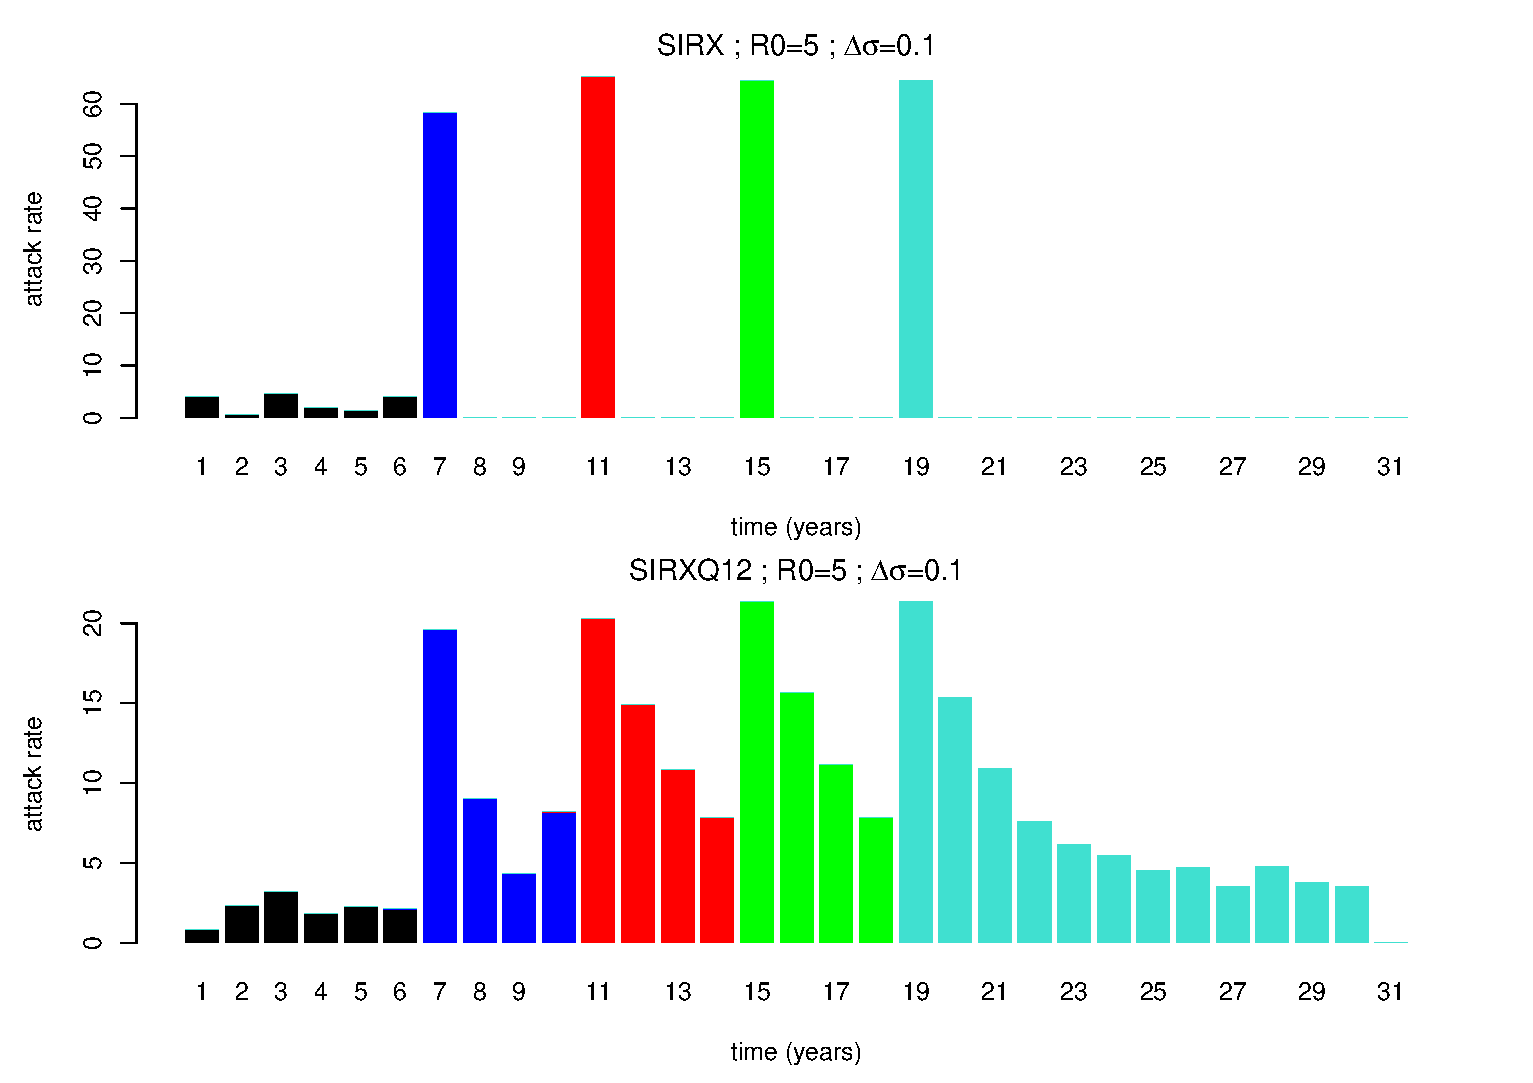
\includegraphics[width=0.9\linewidth]{texte/article3/graph/attack_r05.eps}
  \caption{Evolution of the annual attack rates in Paris for a typical
    realisation of the $SIRX$ (top) and $SIRXQ12$ with immune boosting
    (bottom) stochastic metapopulation models. Parameters are
    identical to figure~\ref{fig:world_sirx} except for $R_0=5$ ;
    $\sigma_X=0.1$ ; $\Delta \sigma=0.1$.}
  \label{fig:attack5}
\end{figure}




% Increasing $R_0$ can improve this situation especially in the $SIRS$
% limit where the effect of cross immune boosting is higher.


\section{Discussion}
\label{sec:discussion}
%a modifier de place


%However, it is difficult to know
%to what extent table \ref{tab:drift_values} estimates are relevant as
%the average antigenic distance between the center of consecutive
%antigenic clusters was used as a measure of a typical antigenic
%distance during antigenic cluster transition for table
%\ref{tab:drift_values} calculation. Given that antigenic cluster are
%relatively ``large'' in antigenic space \citep{Smith2004}, our
%estimates can be overestimated.


%Enfin on sait que: en 29 ans on a mis a jours 19 fois le vaccin (Hay
%2001) soit tous les 1.53 ans (faudrait mettre à jour cette stat)
%Tout d'abord juste pour vérifier:
%si on prend les data de smith on trouve que il faut mettre a jour le
%vaccin en moyenne tous les: 2/1.2=1.67 ans
%avec celle de Russel: tous les 2/2.13=0.94 ans 
%c'est cohérent avec les mise à jour tous les 1.53 ans (heureusement)

%Wild birds and especially aquatic birds of the orders Anseriformes and
%Charadriformes constitute the natural reservoir of influenza A
%viruses. In their reservoir, Influenza A virus possess antigenically
%and genetically diverse hemagglutinin (HA) and neuraminidase (NA)
%subytpes which includes all known influenza A virus HA (16 variants)
%and NA (9 variants). At least 103 of the possible 144 type A influenza
%virus HA-NA combinations have been found in wild birds
%\citep{Dugan2008}
%
%In contrast, influenza B and C virus are mostly present in human. As
%reported by \citet{Webster1992}, modern influenza B and C virus do not
%reassort with influenza A viruses and leave viable progeny. To explain
%this genetic incompatibility, there had to be little or no gene flow
%between human and avian virus gene pools after the introduction of
%avian-derived influenza viruses into human hosts. During a long period
%of isolation, human influenza B and C viruses underwent hosts-specific
%adaptive evolution and accumulated enough mutations that reassortant
%virus were no longer viable.

%This proposal suggests that there have been fundamental changes in the
%ecology of human influenza viruses during human history.  For instance
%\citet{Day2006} report that if evolutionary emergence of past
%pandemics has occurred primarily through viral reassortment in humans,
%then thousands of avian influenza virus infections in humans must have
%occurred each year for the past 250 years.  Due to the decreased
%isolation of human and avian virus gene pools, human influenza viruses
%have been prevented from reaching an evolutionary equilibrium with
%their hosts by an irregular infusion of avian virus genes into the
%human virus gene pool.
%

The current naoH1N1 pandemics illustrates the continuous intrusion of
avian (and swine) influenza genes into the human population. For
instance \citet{Day2006} report that if evolutionary emergence of past
pandemics had primarily occurred through viral reassortment in humans,
then thousands of avian influenza virus infections of humans should
have occurred each year for the past 250 years. In this study, we have
proposed a general framework to handle the dynamics of these
successful perturbations resulting generally in influenza subtype
replacement.
%
At the subtype level, a similar replacement dynamics takes place,
antigenic clusters replacing each other every 1 to 8 years. As
antigenic clusters replacement induce strong selective sweeps
\citep{Koelle2006, Rambaut2008}, this process has recently been
proposed as a key factor to restrict an otherwise ever-growing strain
diversity.

At the heart of our framework is the recognition that influenza
antigenic unit (IAU, either antigenic cluster or subtype) are subject
to gradual antigenic drift \citep{Suzuki2008, Shih2007, Russell2008}.
We coupled an implicit treatment of IAU gradual antigenic drift with
\citet{Koelle2009} proposal of modelling rapidly evolving pathogens by
focusing on the tempo of antigenic change instead of genetic changes.
The resulting model called $SIRX$ allows to track the dynamics of a
considerably lower set of IAU than the previously used multi-strains
models. The few number of IAUs enable us to use the comparatively less
restrictive history-based framework with a sate space scaling
exponentially with the number of IAUs.


%Even if 1977 H1N1 reintroduction resulted in coexistence with H3N2,
%strong interaction between the sutype were reported with H3N2 almost
%completely diseapear in the following year despite H3N2 having undergo
%a major antigenic change event the same year


\subsection{The $SIRX$ framework for drifting co-circulating IAUs}

%Our development of a framework for interacting co-circulating
%antigenic unit subject to within unit antigenic drift adapted to
%influenza has conducted to reject status based model as in their
%simplest form they result in immune boosting dynamics that are
%somewhat incompatible with the original antigenic sin response. Such
%behaviour was reported by \citet{Ballesteros2009} in case of the
%$SBRI$ model without within unit gradual antigenic drift that was used
%by \citet{Gog2002, Koelle2006, Koelle2009, Gog2008}. The $SBRS$ model
%does not present this issue in the absence of gradual antigenic drift
%within antigenic unit however, we have shown that its introduction
%induces cross immune boosting. If cross immune boosting precludes to
%use those status based model in the context of influenza, our analysis
%has revealed interesting invasion threshold properties that highlight
%the importance of transient dynamics and of the time interval of
%antigenic units introduction.

The $SIRX$ model represents an intermediate choice between the $SIRI$
``reinfection'' model of \citet{Goekaydin2007} and the $SIRS$
``gradual loss of immunity'' model of \citep{Pease1987}.

We have shown that this model present an invasion threshold and have
derived a sufficient condition (relevant for a large class of model
allowing a flexible shape of the evolution of the probability of
reinfection due to gradual antigenic drift) that ensures the invasion
of a mutant IAU in a population where a resident IAU is at the endemic
equilibrium. In the absence of functional constraints, this sufficient
condition (SC) states that the invasion threshold occurs only if
infection by a given IAU confers less protection against strains
belonging to the same IAU than against a new IAU. Since this condition
seems like paradoxical we have mostly considered parameter range where
this threshold was absent.

We have then shown that IAU replacement area was maximised for
parameters close to the $SIRI$ limit as $g \to \infty$. Particularly,
absolutely no replacement areas were found for the $SIRS$ limit
($\sigma_X=1$). Further analysis will be necessary to establish to
what extent \citep{Goekaydin2007} reinfection model can constitute a
sufficient representation of an IAU subject to gradual antigenic
drift.

The investigation of the transient dynamics of IAUs replacement using
the $SIRX$ model in a realistic worldwide metapopulation context has
largely confirmed our preliminary determinist analysis.  Successful
IAU replacement are possible only for a small range of parameters. In
particular, our analysis corroborate \citep{Goekaydin2007} results
that within IAU the susceptible reduction factor must be smaller but
close to the reinfection threshold $\sigma_{X}\lesssim 1/R_{0}$. Our
most striking result is the high effect of the mutant IAU immune
escape ($\Delta\sigma$) on the attack rate of the first outbreak as
well as on the post-outbreak refractory period. Successful IAU
replacement followed by realistic recurring epidemics occurred only
for small immune escape values ($\Delta\sigma\thickapprox 5\%$). As we
show below in table~\ref{tab:drift_values} current estimates for
antigenic cluster change are higher, on the order of 15\%. For such
high values, the $SIRX$ model leads to dynamics close to pandemic
situation with unrealistic high attack rates at cluster transitions.

\begin{table}[h!tb]
  \centering
  \begin{tabular}{|c|c|c|}
    \hline
    & \citet{Smith2004} & \citet{Russell2008} \\
    \hline
    \citet{Pease1987} & 8.3 $|$ 18.7 & 4.7 $|$ 10.5 \\
    \hline
    \citet{Finkenstaedt2005} & 12.3 $|$ 27.7 & 6.9 $|$ 15.6 \\
    \hline
  \end{tabular}
  \caption{Percentage of immunity escape corresponding to:
    left value : 2 antigenic units change (equivalent to a fourfold difference in
    hemagglutination inhibition (HI) assay titer which is considered
    as a sufficient antigenic difference to warrant a vaccine update)
    right value : the average antigenic distance between the center of
    consecutive clusters (4.5$\pm$1.3 in \citet{Smith2004}).
    Calculation were performed by  using \citet{Smith2004}
    and \citet{Russell2008} estimates of the rate of evolution of
    antigenic drift at the phenotypic level (using hemagglutination
    inhibition (HI) assay titer) (resp. 1.2  and 2.13 unit per year) as well as \citet{Pease1987} and
    \citet{Finkenstaedt2005} inference of the rate of loss of immunity
    following an influenza infection (resp. 5\% and 7.4\% per year).}
  \label{tab:drift_values}
\end{table}


Various factors can mitigate this high sensitivity to $\Delta\sigma$
and we have shown that a functional trade-off between transmission
rate and immune escape ability could greatly help to reduce this gap.
However, this trade-off hypothesis is more difficult to model and will
necessitate additional processes to account for compensatory
mutations. In this context the model of \citet{Gog2008} is a
significant improvement but should be re-analysed without the
limitation induced by the $SBRI$ framework.

We have also shown that the addition of a temporary period of full
protection with immune boosting, as suggested by \citet{Ferguson2003},
could improve the situation mostly by reducing the sharpness of the
epidemics and transforming area where both the invading and the
resident IAUs go extinct into successful replacement area.
%
%Interestingly this effect is particularly present in the $SIRS$ limit
%($\sigma_X=1$) for within IAU antigenic drift rates close to values
%inferred from experiments \citep{Pease1987} or data
%\citep{Finkenstaedt2005} ($1/g \approx 10-25$ years$^{-1}$) and
%$R_0\approx 5$, both parameters values where the effect of immune
%boosting are particularly present. Strikingly for this parameter area,
%and due to the existence of the invasion threshold of eq.
%\eqref{eq:threshold} $\Delta\sigma$ of the order of values reported in
%table~\ref{tab:drift_values} leads to successful IAU replacements.
%
From a more biological standpoint we have shown that there were three
ways to introduce this temporary period. Referring to section
\ref{sec:Q} we think that assumption $Q_{1}$ is biologically
reasonable and empirically supported since it occurs after infection
and that cellular immunity targeted toward conserved proteins is well
known to participate viral clearance \citep{Grebe2008}.
%
By contrast, assumption $Q_{2}$ is less evident as it is unknown to
what extent exposure that do not lead to infection can trigger a
cellular immune response. For the same reason, we doubt on the
relevance of assumption $Q_{3}$ as it concern host with an effective
immunity where efficient long lived antibodies can repress the virus
before viral replication ensure sufficient stimulation to trigger a
cellular immune response. 
%
Recent studies tacking influenza A replacement patterns have
emphasized the need for such temporary full-protective period
(\citet{Ferguson2003,Minayev2008,Minayev2009,Tria2005}) without
precisely explaining the underlying biological assumptions. Our study
reveals a significant effect of assumption $Q_{2}$, and calls for
better clarifications before using $Q_{2}$ and especially $Q_{3}$.



%For instance, \citet{Minayev2008,Minayev2009} refer to
%\citet{Ferguson2003} while introducing a short-lived
%strain-transcending immunity. Looking more precisely to their
%equations reveals that they use the assumption $Q_{1}$, a variant of
%the assumption $Q_{2}$ (due to the way the host's immune repertoire is
%updated following exposure) and the more problematic assumption
%$Q_{3}$. Moreover, it seems like there is an inconsistency in their
%equations when introducing this temporary strain-transcending
%immunity. Equation $(4.2)$ of \cite{Minayev2009} (\textit{resp.}
%equation $(2.6)$ of \cite{Minayev2009a}) implies that infection can
%come from a strain already in the immune repertoire: in that case host
%does not become infectious yet develops 6 months strain-transcending
%immunity ($Q_{3}$). But the authors also precise that equation $(2.1)$
%in both papers remains unchanged which is inconsistent with equation
%$(4.2)$ (\textit{resp.} $(2.6)$) since equation $(2.1)$ implies that
%hosts can not be infected or develop 6 months strain-transcending
%immunity if they are challenged by strains already in their immune
%repertoire. In other words, equation $(2.1)$ does not support the
%assumption $Q_{3}$ whereas equations $(4.2)$ (\textit{resp.} $(2.6)$)
%does. The direct consequence of this is an overestimation of the force
%of infection for co-circulating strains. Since this temporary
%full-protection plays a crucial role in their model it must be tested
%if this inconsistency modify the epidemiological and evolutionary
%dynamics and by how much. Note also that this inconsistency can only
%be removed by modifying equation $(2.1)$, thus fully supporting
%assumption $Q_{3}$.

Recent analysis (\citet{Kryazhimskiy2007,Ballesteros2009}) have
revealed a similar issue with the multi-strains status-based model
with reduced infectivity ($SBRI$) as introduced by \citet{Gog2002,
  Koelle2006}. \citet{Ballesteros2009} have for instance showed that
the $SBRI$ model results in significant cross immune boosting in
contradiction with the original antigenic sin \citep{Kim2009}. The
$Q_2$ and $Q_3$ mechanism discussed previously are somewhat comparable
to the cross immune boosting induces by the $SBRI$ with the important
difference that boosting is only temporary (but strain transcending)
and not mediated by a lifelong acquisition of effective immunity to
antigenically distant strain in better agreement with the original
antigenic sin.

In summary, our analysis reveals that the core of the replacement
dynamics of drifting IAU (and therefore of selective sweep as the main
mechanism of strain diversity reduction \citep{Koelle2006}) is already
present in the simple $SIRX$ model but that this model lacks a
mechanism to reduce the sharpness of the epidemics following IAUs
transitions. Such mechanisms could refer to functional constraints or
short-lived strain-transcending immunity with immune boosting although
this latter assumption call for more empirical evidence.


We also suggest that introducing an additional source of heterogeneity
in our model would greatly improve its ability to reproduce IAU
replacement as observed in data. It will be necessary for instance to
relax the assumption of global mixing at the patch (city) level.
Before such an analysis we think that our results cannot be used to
infer level of heterotypic partial cross-immunity as the previously
highlighted strong sensitivity to immune escape can induce important
overestimation of this parameter of tremendous importance for public
health and pandemic preparedness. By focusing on the phenotype level,
the $SIRX$ framework presented here and its mathematical structure is
particularly adapted to be used with recently developed ``plug and
play'' inference technique \citep{Ionides2006, Toni2009}. Such an
analysis will be valuable to disentangle between the various process
previously described. Particularly, we wonder to what extent complex
immune boosting mechanisms ($SBRI$ model or $Q123$) are still
necessary in a more heterogeneous local spatial context.


\subsection{Noisy gradual antigenic drift or punctuated immune escape}

As a last point, in its current form the presented models given their
high sensitivity to immune escape of the mutant tends to support noisy
gradual antigenic drift instead of strong punctuated immune escape. It
is striking to observe how the $SIRX$ model or especially the $SIRXQ_{12}$
model with immune boosting perturbed with small immune escape (of
the order of 5\%) produced by IAU transitions are able to
successfully reproduce observed influenza time series both
qualitatively and quantitatively. \citet{Finkenstaedt2005} analysis of
French ILI data tends also to support this conclusion of noisy gradual
antigenic drift as their inferred immune escape parameters are far
lower than values expected during antigenic cluster transitions even
with the presence of a scaling exponent to handle deviation from
homogeneous mixing. Given the recent discussion on the fact that
influenza antigenic evolution is punctuated or gradual (\textit{e.g}
\citep{Wolf2006, Shih2007, Suzuki2008}) and the recent discovery that
purely gradual antigenic drift is sufficient to induce strong epidemic
variability due to non linear dynamics effects (Ballesteros et al 2009
, submitted), the use of the statistical framework described
above will be of tremendous interest to gain definitive insights with
a mechanistic basis on these long standing questions.

%sinon discutter des parametres
%bcp de cross immuntiy pour les pandemies ???
%biais de loi d'action de masse ?

%%

\section*{Acknowledgements}
This work was partially funded by the R\'egion Ile-de-France and the
“ANR-Agence Nationale de la Recherche – The French National Research
Agency” under the project ANR 05SEST01802 BIOSCOPE.



%%% Local Variables: 
%%% mode: latex
%%% TeX-master: "../../phD"
%%% End: 


\clearpage
\newpage
\thispagestyle{empty}
\null
\newpage

%
%
%\clearpage

\chapter{Discussion}

\begin{quote}
  “I am sure that what any of us do, we will be criticized either for
  doing too much or for doing too little... If an epidemic does not
  occur, we will be glad. If it does, then I hope we can say... that we
  have done everything and made every preparation possible to do the
  best job within the limits of available scientific knowledge and
  administrative procedure.”

  —US Surgeon General Leroy Burney, Meeting of the Association of
  State and Territorial Health Officers, August 28, 1957
\end{quote}

\vspace{2cm}

Nous avons vu en introduction que la prise en compte de la variation
antigénique à l'échelle d'une infection humaine permettait
d'appréhender les différentes trajectoires évolutives ayant mené aux
principales maladies infectieuses humaines. Une des questions à
l'origine de ce travail concernait les conséquences populationnelles
de la variation antigénique en s'appuyant sur le cas des épidémies de
grippe A dans la population humaine. Nous avons vu qu'à cette échelle,
l'immunité de la population est le principal facteur qui structure
cette diversité antigénique et avons cherché à développer des modèles,
les plus simples possibles, pour pouvoir étudier de manière précise la
boucle de rétro-action entre immunité des populations, évolution
virale et dynamique épidémiologique.


\section{Résumé des principaux résultats}

Notre première étude s'est ainsi intéressée aux répercussions des
hypothèses effectuées pour décrire les systèmes multi-souches. Elle a
été largement motivée par le changement de paradigme concernant le
mode d'évolution des propriétés antigéniques de la grippe introduit
par l'article de \citet{Koelle2006} et le débat qui a suivi visant à
déterminer si cette évolution était ponctuée ou plus graduelle. D'une
manière remarquable, l'échappement ponctué à l'immunité de la
population induit des balayages sélectifs capables de rendre compte
des phylogénies observées pour HA1 ainsi que des dynamiques
épidémiologiques. De plus, dans ce contexte, une période d'immunité
temporaire totale agissant quelles que soient les souches ou les
sous-types rencontrés n'est pas nécessaire pour réduire la diversité
virale. D'un point de vue théorique, le changement est considérable
car on passe d'un système où la diversité virale est contrôlée par un
mécanisme de densité dépendance directe à un système où elle est
contrôlée par les dynamiques transitoires de remplacements. Nous avons
montré qu'en réalité cette différence était un peu moins marquée. En
particulier, nous avons mis en évidence que les dynamiques du modèle
utilisé par \citet{Koelle2006} (SBRI) différaient grandement de celles
produites par les autres modèles utilisés pour décrire les systèmes
multi-souches. Au coeur de cette divergence se trouve la combinaison
de l'hypothèse d'une immunité polarisée avec le postulat que
l'immunité croisée agit en réduisant totalement l'infectiosité. Cette
combinaison implique que des individus complètement immunisés pour une
souche donnée peuvent tout de même se faire réinfecter par celle-ci
(il ne deviennent néanmoins pas infectieux) et ainsi, qu'ils
bénéficient à chaque fois d'une chance d'acquérir une protection
totale pour les souches immunologiquement réactives avec la souche
rencontrée. Ce processus (absent dans tous les autres modèles étudiés)
induit une immunité croisée beaucoup plus prononcée et tempère alors
l'échappement à l'immunité ayant lieu lors d'un changement de cluster
antigénique. Cette immunité additionnelle acquise grâce aux
réinfections favorise le remplacement de l'ancien cluster résidant par
le cluster émergeant. Nous avons montré que ce processus de
réinfection avec extension du répertoire immunitaire lors d'exposition
aux souches auxquelles l'hôte est totalement immunisé (sans qu'il
devienne infectieux) est largement contradictoire avec le péché
antigénique originel (OAS). L'importance du péché antigénique originel
a par ailleurs été soulignée récemment dans un article de
\citet{Kim2009} mettant fin à la polémique soulevée par les travaux de
\citet{Wrammert2008}. Devant l'incapacité des autres modèles
n'incorporant pas ce processus à reproduire des dynamiques
transitoires mimant qualitativement des changements de clusters, nous
avons voulu savoir dans quelle mesure un modèle basé sur un scénario
de dérive antigénique graduelle permettait de décrire d'une manière
satisfaisante les données dont on dispose.

La théorie de l'échappement de l'immunité ponctuée offre un mécanisme
intuitif pour expliquer la variabilité des épidémies de grippe
observées dans la zone tempérée, les plus grands échappements à
l'immunité induisant de plus grandes épidémies. Étant donnés nos
résultats précèdents, nous avons cherché à déterminer dans quelle
mesure ce signal épidémiologique pouvait être un indicateur fiable des
variations ponctuelles d'échappement à l'immunité. Nous avons donc
regardé si le modèle le plus simple possible, mimant une dérive
antigénique graduelle pouvait générer des dynamiques similaires à
celles observées dans la zone tempérée. Cette étude a révélé que ce
modèle déterministe produisait des dynamiques chaotiques mais avec la
propriété remarquable d'être régulière. Ainsi notre modèle minimal
génère des épidémies de tailles différentes chaque année, avec une
légère variabilité dans la date de départ de l'épidémie, et ce avec un
échappement à l'immunité parfaitement graduel, chaque individu ayant
une probabilité constante par unité de temps de redevenir susceptible.
Le caractère chaotique de la dynamique illustre en outre que même dans
ce cas idéal, où la dérive antigénique est parfaitement prévisible, il
existe un niveau d'indétermination fondamentale à notre capacité à
prédire l'état du système. De manière intrigante, cet horizon de
prédictabilité (déterminé par l'exposant de Lyapunov dominant) est de
l'ordre de grandeur de 3 ans, durée moyenne de changement des clusters
antigéniques. Nous avons également montré que cette dynamique, dite
UPCA (pour Uniform Phase with Chaotic Amplitude), se produisait dans
de larges zones de paramètres réalistes pour la grippe, y compris pour
les paramètres que nous avons inférés à partir de deux jeux de données
et qu'elle était robuste à différentes formes de perturbations (y
compris la co-circulation de différents sous-types dans un contexte
spatial réaliste). Ce modèle pourrait être en mesure de fournir une
explication au constat que les saisons les plus sévères de grippe
saisonnière ne sont pas toujours associées à des nouveautés
antigéniques marquées et peuvent avoir lieu durant des années où un
même cluster antigénique reste présent. Les épidémies de 1989-1990 au
Royaume Uni ou de 1999-2000 aux USA en sont des illustrations
remarquables \citep{Viboud2006b} et restent à ce jour à notre
connaissance inexpliquées.

Ce résultat, nous a amené à revisiter la théorie de l'évolution
antigénique ponctuée de la grippe et à développer un formalisme
suffisamment tractable et général pour pouvoir être utilisé dans un
cadre d'inférence statistique. Pour ce faire nous avons utilisé
l'approche de \cite{Koelle2009} qui se focalise uniquement au niveau
du phénotype. Dans le contexte de la grippe, les clusters antigéniques
constituent alors un niveau d'abstraction privilégié. Toutefois, étant
donné l'importance de la dérive antigénique graduelle au sein d'un
cluster antigénique \citep{Shih2007, Russell2008}, nous l'avons
incorporée. Nous avons choisi de le faire d'une manière implicite,
évitant encore de décrire de nombreuses souches. Ces simplifications
nous ont permis de réduire considérablement le nombre de variables
d'état nécessaires pour définir le système et ainsi de nous affranchir
de la nécessité de devoir se limiter à des formalismes où le nombre
d'équations augmente linéairement avec le nombre de souches
(typiquement le modèle SBRI). A une autre échelle, ce formalisme
permet aussi de décrire la dynamique de sous-types de grippes et donc
d'étudier les conditions menant à leur remplacement durant les
pandémies. L'analyse de ce système nous a conduit à un résultat
surprenant. Il est en effet apparu impossible de pouvoir reproduire
des remplacements de clusters antigéniques pour les distances
antigéniques réalistes qui séparent ces clusters. Ce résultat pourrait
signifier que l'évolution antigénique de la grippe est plus graduelle
qu'on ne le pense car des échappements ponctués à l'immunité de la
population produisent des épidémies trop violentes suivies de trop
longues périodes réfractaires pour être comparable aux données.
L'étude de \citet{Russell2008} utilisant un nombre beaucoup plus élevé
de prélèvements que celle de \citet{Smith2004} (plus de 13000 face à
273) fournit quelques éléments de réponse allant dans le sens d'une
dérive antigénique essentiellement graduelle bien que la période de
leur étude (2002-2007) ne soit pas marquée par des changements de
clusters antigéniques conséquents. Ce résultat surprenant peut aussi
traduire l'importance des contraintes fonctionnelles, largement
reconnue que ce soit sur le plan théorique \citep{Belshaw2008} ou sur
le plan empirique \citep{Rambaut2008}. Ces contraintes pourraient
compenser le gain de fitness relative acquis par un nouveau cluster
antigénique échappant à l'immunité de la population et ainsi éviter de
trop grandes épidémies. Nous avons aussi considéré d'autres hypothèses
et montré qu'une période temporaire d'immunité totale (classe $Q$)
pouvait améliorer la capacité de notre modèle à reproduire les
données, particulièrement si celle-ci est associée à un mécanisme de
``boosting'' immunitaire et des $R_0$ suffisant élevé pour que ce
``boosting'' ait un effet considérable. Dans ces conditions, les
individus partiellement protégés chez qui la protection partielle
suffit à éviter l'infection se retrouvent quand même dans la classe
$Q$. D'une manière plus classique, tous les individus infectés se
retrouvent temporairement dans cette classe après guérison. Ce
processus permet ainsi de réduire le nombre de susceptibles
disponibles pour les nouveaux variants antigéniques et tempère alors
l'intensité de l'épidémie faisant suite à un changement de cluster. La
classe $Q$ avec mécanisme de ``boosting'' rend donc les remplacements
possibles de deux façons : en augmentant l'interaction compétitive
entre les souches mais surtout, en tempérant les épidémies. Introduit
sous cette forme, la classe $Q$ n'est pas si différente du processus
``caché'' induit par le modèle $SBRI$ mis en évidence au chapitre 2.
Une différence de taille existe cependant entre ces 2 façons de
``booster'' l'immunité: la classe $Q$ ne la ``boost'' que
temporairement et sans mise à jour du répertoire immunitaire des hôtes
ne succombant pas à l'infection, tandis que le modèle SBRI induit des
extensions du répertoire immunitaire définitives lors d'expositions
aux souches auxquelles l'hôte est totalement immunisé sans qu'il
devienne infectieux, en désaccord avec l'OAS. Par ailleurs, là où le
``boosting'' est systématique avec la classe $Q$, il devient dépendant
de la distance antigénique pour le modèle $SBRI$. Si la mise en
évidence de ces mécanismes de ``boosting immunitaire'' constitue un
résultat intéressant, on ne peut toutefois pas exclure un rôle
important de l'hétérogénéité spatiale pour tempérer l'intensité des
épidémies.

%correlation R0 derive antigénique. avertissement état immunitaire peut
%varier d'une pop à une autre viboud smoldering pand. peut induire des
%biais considérable dans l'estimation de R0.



%calculer l'effet de la classe $Q$.



% abstract papier 3: finally, we show that both koelle and fergusion
% theory share an unpreviously recognised point by relying on the
% decisive assumption of cross immune boosting, a process during which
% already immunized hosts can gain additional cross protection without
% becoming infectious following additional exposure.

\section{Perspectives}

Le formalisme développé dans le chapitre 4 est suffisamment tractable
pour être couplé à une approche d'inférence statistique et de
sélection de modèles. Nous pensons donc qu'il permettra de mettre en
avant les processus clés impliqués dans la phylodynamique de la
grippe. En particulier, nous espérons pouvoir déterminer dans quelle
mesure les processus complexes de ``boosting'' immunitaires sont
nécessaires en présence d'une hétérogénéité spatiale locale accrue.
Cela nous semble particulièrement important étant donné que, dans le
contexte de la théorie de l'échappement à l'immunité ponctué, le rôle
primordial des processus de ``boosting'' immunitaire (classe $Q$,
modèle SBRI), semblent être de tempérer les épidémies. En effet, les
modèles sans ``boosting'' immunitaire induisent suffisamment de
compétition entre les clusters antigéniques pour provoquer des
balayages sélectifs lors de l'apparition de nouveaux clusters, mais
ils produisent alors des épidémies trop violentes suivies de trop
longues périodes réfractaires pour être réalistes. A ce titre, les
approches visant à prendre en compte simplement l'hétérogénéité
spatiale à une échelle locale sous la forme d'exposants sur les termes
de la loi d'action de masse sont un outil précieux \citep{Liu1987,
  Roy2006}. De plus amples travaux sont nécessaires dans ce domaine
pour mieux comprendre le rôle de ces exposants et déterminer s'ils
sont à même de mimer implicitement l'effet des réseaux de contacts
complexes de la population humaine.

En attendant ces confirmations, nos résultats révèlent que les
processus d'acquisition de l'immunité à l'echelle individuelle peuvent
avoir une importance considérable à l'échelle de la population. En
particulier il nous apparaît essentiel que les possibilités d'un
``boosting'' immunitaire régi par la classe $Q$ soient clarifiées
empiriquement. Notre travail suggère spécialement la nécessité d'une
meilleure compréhension de la façon dont interagissent les mécanismes
du péché antigénique originel (OAS) et les processus immunitaires
aboutissant à la mise en place d'une immunité cellulaire conférant une
protection totale hétéro-sous-typique mais limitée dans le temps. Si
ces 2 processus sont bien reconnus, que ce soit chez les modèles
animaux \citep{Grebe2008, Kim2009} ou lors d'études épidémiologiques
chez l'homme \citep{Slepushkin1959, Epstein2006}, les mécanismes
impliqués pour leur élicitation restent en partie à découvrir.

L'étude de \citet{Kim2009} offre une perspective intéressante à ce
sujet car les auteurs proposent un mécanisme pour l'OAS. Leur étude
suggère en effet que l'OAS pourrait être dû à une compétition entre
les lymphocytes B mémoires partiellement réactifs et les lymphocytes B
naïfs. Ceci se comprend en considérant une infection séquentielle par
deux souches ($s1$ et $s2$) immunologiquement partiellement réactives.
Comme le révèle l'étude de \citet{Kim2009}, la première infection
génère des anticorps spécifiques à $s1$ seulement, ainsi que des
anticorps partiellement réactifs à $s2$. Cependant, la situation est
différente lors de la seconde infection par la souche $s2$ car à
présent, les anticorps partiellement réactifs envers $s2$, générés
lors de l'infection par $s1$, dominent la réponse immunitaire et
pénalisent le déclenchement d'une nouvelle réponse spécifique à $s2$.
Ce phénomène pourrait s'expliquer par le fait que l'hemagglutinine
permet un accrochage des virus à l'ensemble des lymphocytes B quel que
soit leur récepteur caractéristique (BCR) via l'acide sialique. Cela
pourrait favoriser la capacité des lymphocytes B à présenter les
antigènes spécifiques des virus entrés en contact avec eux et ainsi
biaiser la présentation des antigènes spécifiques en faveur des
lymphocytes B, au détriment des cellules dendritiques. Ce mécanisme
pourrait conduire à des signaux d'activation sub-optimaux favorisant
la réponse immunitaire médiée par les lymphocytes B mémoires seulement
partiellement adaptés à $s2$ par rapport à l'activation de lymphocytes
B naïfs. Dans ce contexte, l'infection par $s2$ conduira à une charge
virale considérable au sein de l'hôte, bien que réduite par rapport à
celle ayant lieu dans un hôte naïf \citep{Kim2009}.

Au vu de ce mécanisme, dans le cas où l'OAS favorise une infection, il
est réaliste de considérer que la composante cellulaire de la réponse
immunitaire sera déclenchée pour éliminer le virus, conférant ainsi
une protection totale de courte durée \citep{Grebe2008}. La
combinaison de l'OAS et de la classe $Q$ sans ``boosting''
immunitaire, se comprend donc relativement bien lorsqu'une exposition
par une souche proche se traduit par une infection. La situation est
plus délicate dans le cas du ``boosting'' immunitaire ayant lieu
lorsque l'exposition ne conduit pas à l'infection. Dans ce dernier
cas, étant donné que l'hôte ne sera pas infectieux, on sait que sa
charge virale sera relativement faible voire nulle si les anticorps
présents chez l'hôte parviennent à neutraliser les virus très tôt. On
peut donc se demander dans quelle mesure une telle infection est
capable de déclencher une réponse immunitaire cellulaire. S'il a été
montré qu'une vaccination pouvait suffire à déclencher la classe $Q$
\citep{Slepushkin1959}, il est difficile de savoir dans quelle mesure
une exposition n'engendrant pas d'infection peut être comparable à une
vaccination. Lorsque l'OAS s'applique, peut-être que la charge virale
est suffisamment élevée pour tout de même déclencher la classe $Q$,
mais dans ce cas, l'hôte peut-il toujours être considéré non
infectieux ? Une description plus fine entre charge virale et niveau
d'infectiosité serait particulièrement précieuse dans ce contexte.
Nous avons vu en introduction que l'emploi de modèles intra-hôtes
relativement simples pouvait permettre de décrire cette relation avec
un rôle important de la fonction de transmission \citep{King2009}. La
présence de nombreux individus asymptomatiques est en outre une
incitation de plus pour regarder plus précisement dans cette direction
\citep{Carrat2008}.


Nous avons par ailleurs mis en évidence (annexe D) que les processus
d'acquisition de la réponse immunitaire pouvaient être fortement
variables selon que les hôtes soient naïfs ou pas. Pour se faire, nous
nous sommes intéressés à la première apparition de H3N2 sur l'île
isolée de Tristan da Cunha. Cette population où H3N2 est apparu
seulement en 1971, soit 3 ans après la pandémie de ce sous-type,
présente la particularité remarquable d'être exceptionnellement
susceptible à la grippe, principalement en raison du très faible
nombre d'expositions des habitants de cette île isolée. De façon tout
à fait surprenante, l'introduction de H3N2 dans cette île a produit
deux épidémies successives de grippe (confirmée par des analyses
sérologiques) séparées de moins d'un mois. Parmi les 284 habitants,
96\% ont subi au moins une infection et 32\% ont été infectés à deux
reprises, l'essentiel des réinfections ayant lieu lors de la seconde
vague. Nous avons cherché à déterminer quels processus étaient à même
de rendre compte de cette situation. Nous avons adopté une approche de
comparaison de modèles en mettant en contraste trois processus :
\begin{itemize}
\item La nécessité d'infections multiples avant de développer une
  immunité protective de longue duré (comme mise en évidence par
  \citet{Mathews2007}).
\item Une protection seulement partielle après la première infection.
\item Une mutation permettant au virus d'échapper à l'immunité
  contractée lors de la première vague.
\end{itemize}

Les résultats de cette analyse, décrits en détail en annexe D, nous
ont permis de valider la première de ces hypothèses. Ainsi, ces deux
vagues pandémiques sont en accord avec un modèle où seulement 50\% des
individus développent une immunité de longue durée après la première
attaque.  Il est difficile de savoir dans quelle mesure ce résultat
est généralisable, cependant, nous pensons qu'un processus similaire
pourrait avoir lieu de manière courante chez les individus
immunologiquement naïfs et donc typiquement chez les enfants.

Ce résultat incite à prendre en considération le rôle des infections
répétées. Si nous avons beaucoup parlé de distance antigénique dans ce
travail de thèse, il nous semble important de clarifier par la suite
le rôle du nombre d'infections dans l'acquisition d'une réponse
immunitaire de plus en plus protégeante et robuste à la dérive
antigénique virale. La réponse immunitaire cellulaire, dirigée contre
des protéines conservées à un rôle considérable dans ce domaine et les
infections multiples, en stimulant de plus en plus cette immunité,
pourraient peut-être à terme la rendre plus persistante, contrecarrant
ainsi l'échappement viral dû à la dérive antigénique (et favorisé par
l'OAS favorisant à son tour les infections répété et donc la
possibilité d'augmenter une réponse immunitaire fortement
réactive...). La suggestion que des infections naturelles (par
opposition au vaccin) répétées par la grippe dans le jeune âge
permettent une meilleure protection contre la grippe une fois âgé (en
plus de poser des questions passionnantes sur les politiques
vaccinales à adopter) incite fortement à regarder de plus près ces
questions \citep{Carrat2006a}.


\vspace{2cm} 

Une description fine des processus immunologiques peut avoir des
répercussions importantes à l'échelle de la population. La complexité
des modèles prenant en compte l'interaction de différents types
antigéniques à l'échelle de la population rend pour le moment
cependant difficile leur couplage avec des modèles décrivant la
relation entre le système immunitaire et la population virale au
niveau intra-hôte. A terme on peut toutefois espérer parvenir à
trouver un formalisme adapté à cette tâche, peut-être sous la forme
intermédiaire entre modèles individus centrés et systèmes dynamiques.
Un tel cadre unifié nous permettrait alors d'appréhender de façon
globale les interactions complexes et multi-échelles entre processus
immunologiques, épidémiologiques et évolutifs.


%A terme, o
%
%
% Les études de
%\citet{Lange2009}, \citet{Read2006} et \citet{King2009} illustrent
%particulièrement bien comment la combinaison de processus
%immunologiques à l'echelle intra-hote, couplé avec des processus
%épidémiologiques ainsi que des contraintes physoliogique permet de
%rendre compte des rétroactions entre dynamique épidémiologique et
%évolutive.
%
%importance du seuil intra hote pour invalider le SBRI...
%
%Il est admis que les anticorps préexistant jouent un rôle clef dans la
%protection contre les infections grippales. Cependant,
%\citet{Wrammert2008} ont montré récemment que les anticorps produit de
%novo par les cellules sécrétrices d'anticorps (ASC) relativement tôt
%suite à une vaccination (pique au 7eme jour) pouvait aussi avoir un
%rôle important en produisant une grande quantité d'anticorps
%spécifique aux antigénes présenté et ce apparemment sans être affecté
%par le péché antigénique originel (les anticorps produits ayant autant
%d'affinité si ce n'est plus avec les souches du vaccin actuel qu'avec
%celles des vaccins précédents. D'une manière remarquable les ASC ayant
%produit ces anticorps ont accumulé plus de mutations somatiques que
%n'importe quel population normal de lymphocytes B suggérant que ces
%cellules proviennent de lymphocyte B ``mémoires'' ayant accumulé des
%mutations sur les précédents cycles d'activations
%\citep{Wrammert2008}. Indépendamment des perspectives intéressantes de
%thérapie fournie par cette découverte cela peut fournir un argument
%allant dans le sens d'une réponse immunitaire multiplicative.
%
%
%
%discussion de la classe Q
%
%\cite{Slepushkin1959}
%\cite{Epstein2006}
%\cite{Carrat2006}
%\cite{Grebe2008}





%Comme l'a écrit Michel Tibayrenc dans l'éditorial du premier numéro du
%journal Infection, Genetics and Evolution nous vivons donc ``l'age
%d'or de la génétique mais l'age sombre des maladies
%infectieuses''. Cet ``age d'or de la génétique'' s'accompagne d'une
%augmentation sans précédent des capacités de calculs, plus que jamais
%nécessaire pour pouvoir analyser les données complexes fourni par le
%sequencages d'isolat provenant du monde entier \citep{Holmes2007}.
%Cette situation offre l'opportunité jamais atteinte auparavant de
%pouvoir pouvoir étudier de l'échelle intra-individuel à planétaire
%comment émerge la boucle de retro-action éco-évolutive façonnant les
%maladies infectieuses.



%%% Local Variables: 
%%% mode: latex
%%% TeX-master: "../phD"
%%% End: 


\clearpage
\newpage
\thispagestyle{empty}
\null
\newpage

%\cleardoublepage

\appendix

\chapter{Supporting Information: Influenza A gradual and
  epochal evolution: insights from simple models}

\author{Sébastien Ballesteros$^{1,*}$, Elisabeta Vergu$^{2}$, Bernard
  Cazelles$^{1,3}$}

%\date{}

%\renewcommand{\figurename}{Figure S}
%\renewcommand{\tablename}{Table S}

~ \\
$^1$UMR 7625  (UPMC, ENS, AgroParisTech, CNRS), Ecole Normale Supérieure, Unit of Eco-Evolutionary Mathematics,  46 rue d'Ulm, F-75230 Paris Cedex 05, France. \\
$^2$~INRA, UR341 Mathématiques et Informatique Appliquées, F-78352 Jouy en Josas, France \\
$^3$~UMMISCO UMI 209 IRD-UPMC, 93142 Bondy, France

~ \\
$^*$\textit{Corresponding author}:  \\
E-mail: sebastien.ballesteros@biologie.ens.fr

\section{Reaction scheme for the $SBRI$ model}

\begin{table}[!h]
\center
	\begin{tabular}{ll}
		reaction & rate \\
		birth\\
		$R_\varnothing \rightarrow R_\varnothing +1$ & $\mu N$ \\
		death\\
		$R_\varnothing \rightarrow R_\varnothing -1$ & $\mu R_\varnothing$ \\
		$R_1 \rightarrow R_1-1$ & $\mu R_1$ \\
		$R_1 \rightarrow R_2-1$ & $\mu R_2$ \\
		$R_{12} \rightarrow R_{12}-1$ & $\mu R_{12}$ \\
		$I^1 \rightarrow I^1-1$ & $\mu I^1$ \\
		$I^2 \rightarrow I^2-1$ & $\mu I^2$ \\
		recovery \\
		$I^1 \rightarrow I^1-1$ & $\nu I^1$ \\
		$I^2 \rightarrow I^2-1$ & $\nu I^2$ \\
		$I^1$ production and $R_1$ only immunisation from $R_\varnothing$ \\
		$R_\varnothing \rightarrow R_\varnothing-1$ ; $R_1 \rightarrow R_1+1$ ; $I^1 \rightarrow I^1+1$ & $(1-\sigma) \beta_1 R_\varnothing I^1/N$ \\
		$I^2$ production and $R_1$ only immunisation from $R_\varnothing$ \\
		$R_\varnothing \rightarrow R_\varnothing-1$ ; $R_1 \rightarrow R_1+1$ ; $I^2 \rightarrow I^2+1$ & $(1-\sigma) \beta_2 R_\varnothing I^2/N$ \\
		$I^1$ production and $R_{12}$ only immunisation from $R_\varnothing$ \\
		$R_\varnothing \rightarrow R_\varnothing-1$ ; $R_{12} \rightarrow R_{12}+1$ ; $I^1 \rightarrow I^1+1$ & $\sigma \beta_1 R_\varnothing I^1/N$ \\
		$I^2$ production and $R_{12}$ only immunisation from $R_\varnothing$ \\
		$R_\varnothing \rightarrow R_\varnothing-1$ ; $R_{12} \rightarrow R_{12}+1$ ; $I^2 \rightarrow I^2+1$ & $\sigma \beta_2 R_\varnothing I^2/N$ \\
		$I^1$ production and $R_{12}$ only immunisation from $R_1$ \\
		$R_1 \rightarrow R_1-1$ ; $R_{12} \rightarrow R_{12}+1$ ; $I^1 \rightarrow I^1+1$ &  $\beta_1 R_1 I^1/N$ \\
		$I^2$ production and $R_{12}$ only immunisation from $R_1$ \\
		$R_1 \rightarrow R_1-1$ ; $R_{12} \rightarrow R_{12}+1$ ; $I^2 \rightarrow I^2+1$ &  $\beta_2 R_1 I^2/N$ \\
		$R_{12}$ immunity acquisition from $R_1$ by $I^1$ \\
		$R_{12} \rightarrow R_{12}+1$ ; $R_1 \rightarrow R_1-1$ &  $\sigma \beta_1 R_1 I^1/N$ \\
		$R_{12}$ immunity acquisition from $R_1$ by $I^2$ \\
		$R_{12} \rightarrow R_{12}+1$ ; $R_1 \rightarrow R_1-1$ & $\sigma \beta_2 R_1 I^2/N$
	\end{tabular}
	\caption{Reaction scheme for the $SBRI$ model}
	\label{tab:reaction}
\end{table}

In the case of reduced susceptibility ($SBRS$ model), the reaction scheme of table~S\ref{tab:reaction} remains the same except that the last 2 reactions do not occur.


\clearpage

\section{Critical community size for influenza}

\begin{figure}[!h]
  \center
  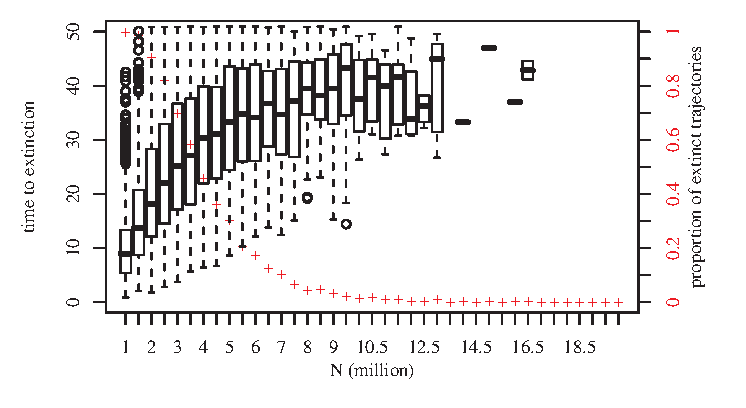
\includegraphics[]{graphs/article1/css_sir.eps}
  \caption{Endemic fadeouts obtained using the $SIR$ stochastic model
    estimated by the distribution of the time to extinction. Red
    crosses represent the proportion of extinct trajectories after
    $T_{max} = 50$ years calculated on 1000 simulations. Initial
    conditions correspond to the endemic equilibrium of the
    deterministic model: $S=200000$, $I=250$ and $R=799750$. Parameter
    values are given in Table~1 (theoretical set).}
\label{fig:ccs}
\end{figure}


\begin{figure}[!h]
  \center
  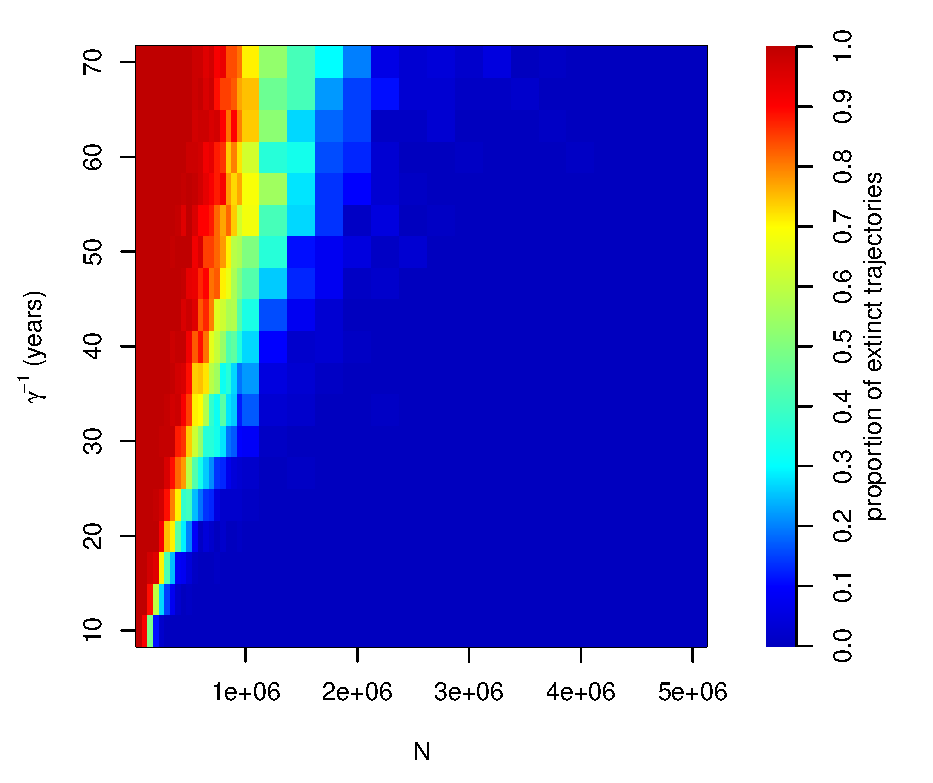
\includegraphics[width=0.5\linewidth]{graphs/article1/ccs_sirs.eps}
  \caption{Effects of gradual antigenic drift on the CCS. We do not
    explicitly model mutant strains resulting from within gradual
    antigenic drift but consider that the emergence of new viral
    strains can be captured by introducing into the model a loss of
    immunity by the host, as originally suggested by Pease (1987).
    Gradual antigenic drift is therefore modelled by a $SIRS$ model
    with demography. Parameter $\gamma$ governs the transition from
    $R$ to $S$, reproducing gradual immune escape. The proportion of
    extinct trajectories after $T_{max} = 50$ years calculated on 100
    simulations is plotted. Initial conditions correspond to the
    endemic equilibrium of the deterministic model. Parameter values
    are given in Table~1 (theoretical set).}
\label{fig:ccs_sirs}
\end{figure}

\clearpage

\section{Complementary results for the theoretical parameters set}

\begin{figure}[!h]
\center
	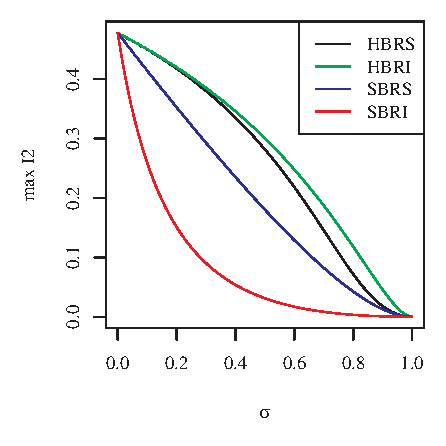
\includegraphics[]{graphs/article1/max_theoretical12.eps}
        \caption{Peak value of the first outbreak of the mutant
          cluster as a function of partial cross-immunity ($\sigma$)
          for the four models studied. Parameter values are given in
          Table 1 (theoretical set). Initial conditions are :
          ${I^1}(0) = {I^1}^*=250.4*10^{-6}$, ${I^2}(0)=10^{-6}$.}
\label{fig:max_theo}
\end{figure}


\begin{figure}[!h]
  \center
    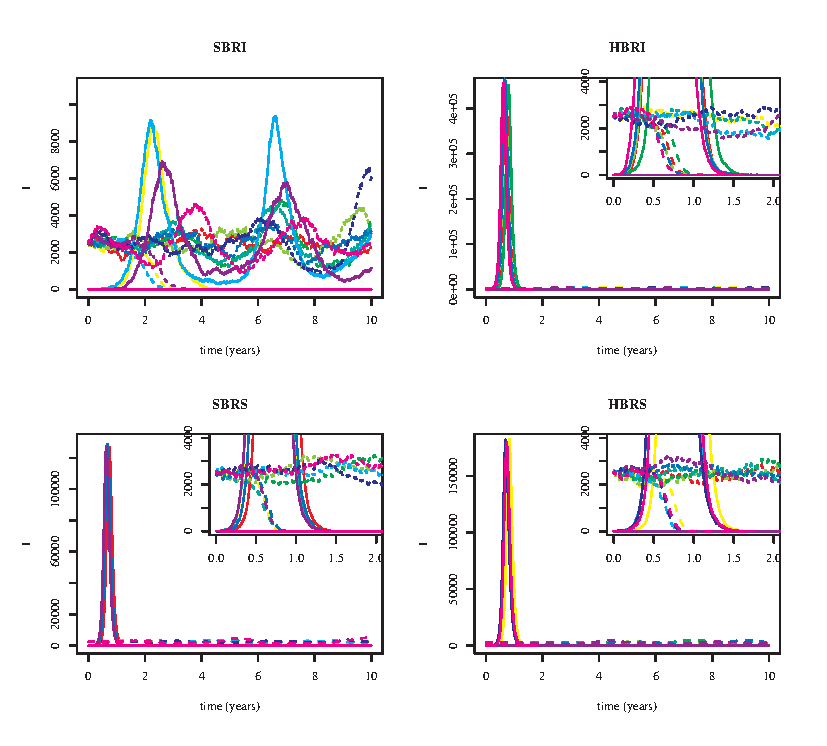
\includegraphics[width=0.8\linewidth]{graphs/article1/traj_sto_drift_theo.eps}
    \caption{Ten realisations of the four stochastic
      models for $\sigma = 0.9$ (punctuated immune escape).
      Realisations are distinguished by different colours. Plain lines
      correspond to infectious hosts for the invader antigenic cluster
      and dashed lines to infectious hosts for the resident antigenic
      cluster.}
\label{fig:sto_drift}
\end{figure}

\begin{figure}[!h]
  \center
	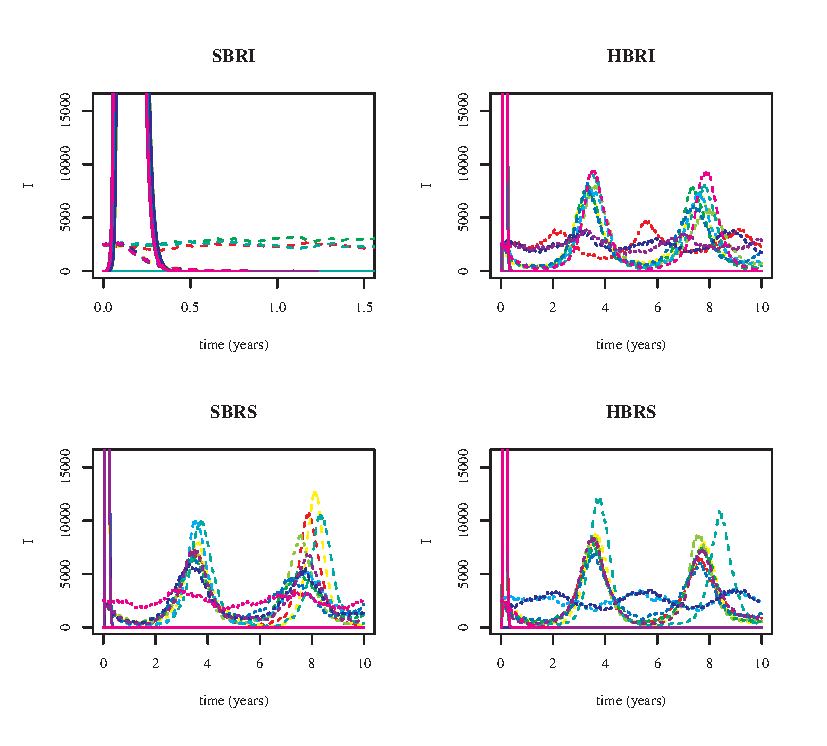
\includegraphics[width=0.8\linewidth]{graphs/article1/traj_sto_shift_theo.eps}
	\caption{Ten realisations of the four stochastic
          models for $\sigma = 0.05$ (antigenic shift). Realisations
          are distinguished by different colours. Plain lines
          correspond to infectious hosts for the invader antigenic
          cluster and dashed lines to infectious hosts for the
          resident antigenic cluster.}
	\label{fig:sto_shift}
\end{figure}


\begin{figure}[!h]
  \center
	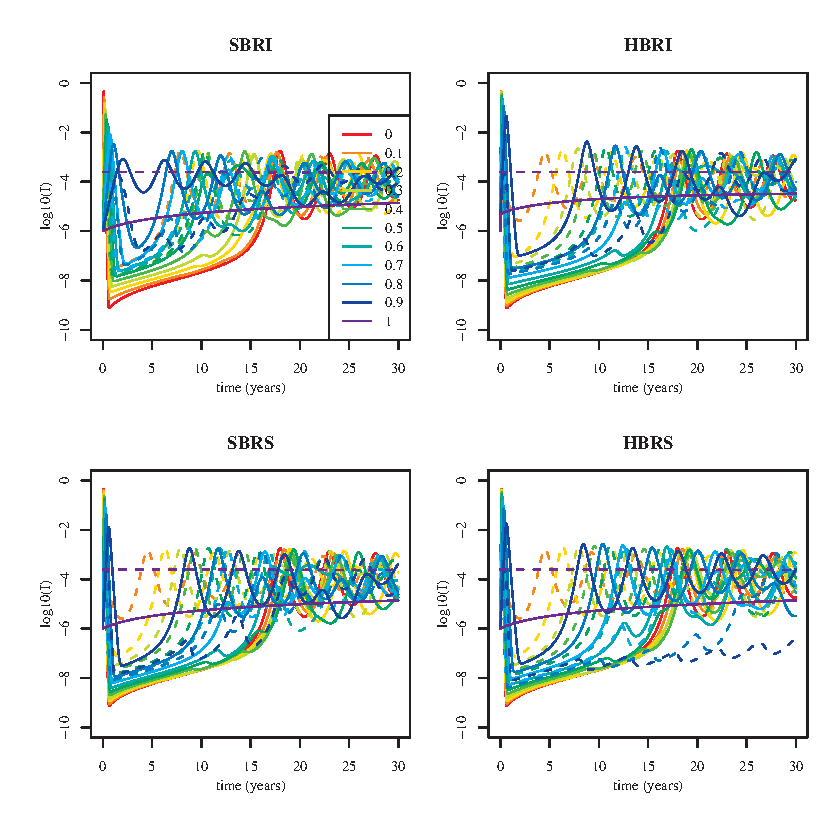
\includegraphics[]{graphs/article1/traj_sir_theoretical_migr8.eps}
	\caption{Transient invasion dynamics for the four two-cluster
          models studied in the presence of external reintroductions
          of infectious hosts. The decimal logarithm of the proportion
          of infectious hosts for the mutant antigenic cluster (plain
          lines) and for the resident cluster (dashed lines) is
          represented as a function of $\sigma$. Colours correspond to
          different partial cross-immunity ($\sigma$) values: from
          $\sigma=0$ (antigenic shift, no cross-immunity) to
          $\sigma=1$ (antigenic drift, full cross-immunity). Parameter
          values are given in Table 1 (theoretical set),
          $mp_i=10^{-8}$. Initial conditions are : ${I^1}(0) =
          {I^1}^*=250.4*10^{-6}$, ${I^2}(0)=10^{-6}$.}
	\label{fig:deter_migr}
\end{figure}

\clearpage


\section{A model for within cluster antigenic drift}

Within cluster antigenic drift is introduced by assuming that viruses
present two parts:
\begin{itemize}
\item a conserved part, identical for both clusters whose phenotype
  cannot evolve.
\item a specific part, subject to slight phenotypic variation
  following quasi-neutral mutation.
\end{itemize}

Partial cross-immunity is provided by the conserved part. Gradual
antigenic drift induces continuous changes of the specific part and,
new specific parts are introduced following immune escape mutations.
We further assume that a primary immune response results in the
acquisition of immune memory toward both the conserved and the
specific parts.

We note $\sigma$ and $\sigma_s$ ($\sigma, \sigma_s \in [0,1]$) the
degrees of protection provided respectively by immunity to the
conserved and the specific part of the virus. We assume additivity of
cross protection with the constraint that $\sigma + \sigma_s \leq 1$.

In case where we assume that within cluster antigenic drift results in
strains diversity rendering intra-cluster immunity only partial, the
previous assumption enables to recover Gökaydin \textit{et al.} (2007)
$SIRI$ model. Reinfections with strains belonging to a cluster for
which hosts have been immunised occur with a reduced probability
$(1-(\sigma+\sigma_s))$. Infections by strains belonging to a mutant
cluster never encountered by the hosts occur with a reduced
probability $(1-\sigma)$

In case where we assume that within antigenic clusters evolution
results in a progressive loss of immunity as proposed by Pease (1987)
($SIRS$ framework) we introduce a parameter ($\gamma$) governing the
rate of antigenic drift. Infections of naive hosts by strains
belonging to cluster $i$ confer full immunity toward strains of
cluster $i$ ($\sigma+\sigma_s=1$, $R_{Ci}$ hosts in figure~8 of the
main text). Antigenic drift affects the specific part of the virus
belonging to cluster $i$ and induces a loss of immunity toward the
specific part after a time governed by a rate $\gamma$ ($R_{Ci} \to
R_C$). $R_C$ hosts can then be reinfected by strains belonging to
cluster $i$ but with a reduced probability ($1-\sigma$) due to
immunity provided by the conserved part. The conserved part also
ensures that $R_{Ci}$ and $R_C$ hosts have a reduced
probability ($1-\sigma$) to be infected by strains belonging to
cluster $j$ (partial cross-immunity).

We formulate the model of figure~7 (main text) using an
$HBRS$ framework and neglecting co-infections in order to compare it
to Gökaydin \textit{et al.} (2007) model.  These assumptions lead to
the following equations:

\begin{align}
\dot{R_\varnothing} &  = \mu -\beta_1 R_\varnothing (I^1_\varnothing +
I^1_{2}) -\beta_2 R_\varnothing (I^2_\varnothing + I^2_{1}) -\mu
R_\varnothing \notag \\
\dot{I^1_\varnothing} & = \beta_1 R_\varnothing (I^1_\varnothing
+I^1_{2}) + (1-\sigma) \beta_1 R_C (I^1_\varnothing +I^1_{2}) -\nu_1
I^1_\varnothing -\mu I^1_\varnothing  \notag \\
\dot{I^1_\varnothing} & = \beta_2 R_\varnothing (I^2_\varnothing
+I^2_{1}) + (1-\sigma) \beta_2 R_C (I^2_\varnothing +I^2_{1}) -\nu_2
I^2_\varnothing -\mu I^2_\varnothing  \notag \\
%
\dot{R_{C1}} &  = \nu_1 I^1_\varnothing -(1-\sigma) \beta_2 R_{C1} (I^2_\varnothing +I^2_{1}) -\gamma_1 R_{C1} +\gamma_2 R_{C12} -\mu R_{C1}  \notag \\
\dot{R_{C2}} &  = \nu_2 I^2_\varnothing -(1-\sigma) \beta_1 R_{C2} (I^1_\varnothing +I^1_{2}) -\gamma_2 R_{C2} +\gamma_1 R_{C12} -\mu R_{C2}  \notag \\
%
\dot{R_C} &  = \gamma_1 R_{C1} + \gamma_2 R_{C2} -(1-\sigma) \beta_1
R_C (I^1_\varnothing +I^1_{2}) -(1-\sigma) \beta_2 R_C
(I^2_\varnothing +I^2_{1}) -\mu R_C   \notag \\
%
\dot{I^1_2} &  = (1-\sigma) \beta_1 R_{C2} (I^1_\varnothing +I^1_{2}) -\nu_1 I^1_2 -\mu I^1_2 \notag \\
\dot{I^2_1} &  = (1-\sigma) \beta_2 R_{C1} (I^2_\varnothing +I^2_{1}) -\nu_2 I^2_1 -\mu I^2_1 \notag \\
%
\dot{R_{C12}} &  = \nu_1 I^1_2 + \nu_2 I^2_1 -\gamma_2 R_{C12} -\gamma_1 R_{C12} -\mu R_{C12}  \notag
\end{align}


\begin{figure}[!h]
  \center
  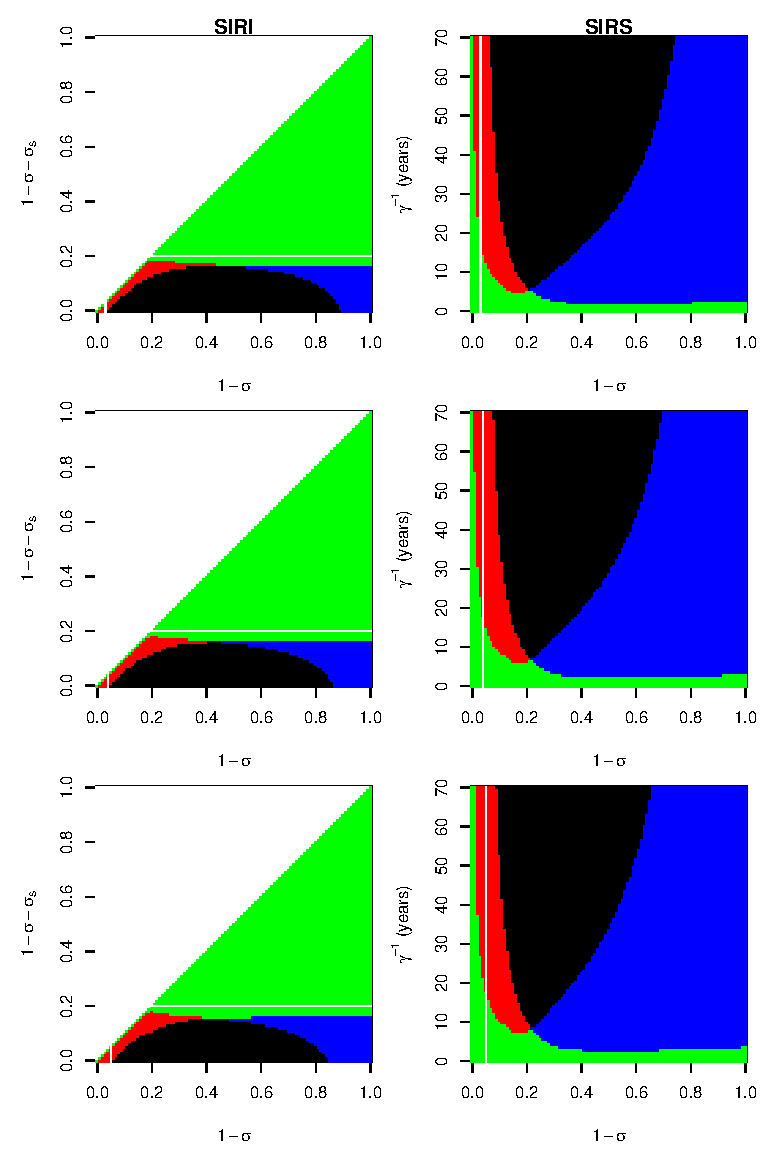
\includegraphics[width=0.5\linewidth]{graphs/article1/within_drift.eps}
  \caption{Effect of the introduction of within cluster
    gradual antigenic drift on the outcome of the invasion of a new
    antigenic cluster. Comparison of the $SIRS$ model (right)
    described in figure~7 and section 4 of the appendix with the
    $SIRI$ model of Gökaydin \textit{et al.} (2007) (left). x-axis
    scale the amount of immune escape achieved by the mutant antigenic
    cluster. y-axis represent a measure of within cluster antigenic
    drift (see section 3 of the appendix for details). Colours: both
    antigenic clusters go extinct (black), the resident cluster only
    goes extinct (successful replacement, red); the mutant cluster
    only goes extinct (blue); no cluster goes extinct (coexistence,
    green). Extinction threshold is set at $N=10^{-6}$ (top panels),
    $N=10^{-7}$ (middle panels) and $N=10^{-8}$ (bottom panels).
    Parameter values are given in Table 1 (theoretical set). The
    horizontal white lines of the right graphs situates the
    reinfections thresholds of the $SIRI$ models
    ($1-\sigma-\sigma_s=\frac{1}{R_0}$). The vertical white lines set
    the highest immune escape intensity ($1-\sigma$) for which the
    same model without within cluster antigenic drift predicts
    replacements.}
\label{fig:within_drift_app}
\end{figure}

\clearpage


\section{Functional constraints}

\begin{figure}[!h]
  \center
  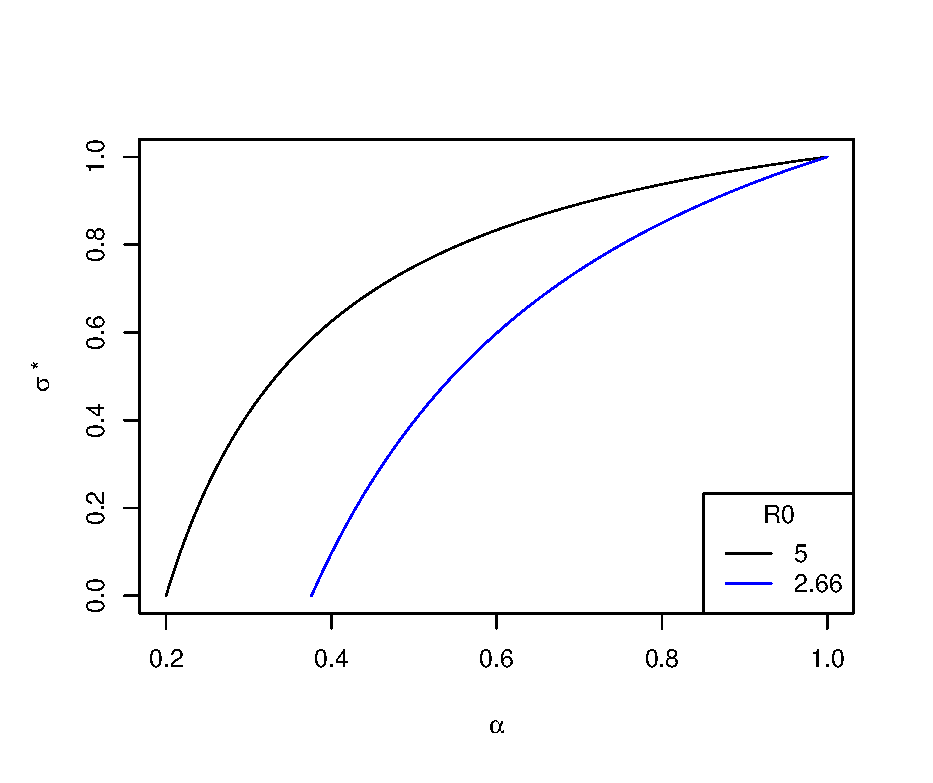
\includegraphics[width=0.5\linewidth]{graphs/article1/constraints.eps}
  \caption{Effect of the fitness reduction (mutant
    transmission rate $\beta$ reduced by a factor $\alpha$) associated
    with immune escape plotted for different values of the resident
    cluster $R_0$. The threshold value of $\sigma$ ($\sigma^*$) needed
    to ensure the mutant cluster invasion is plotted against
    $\alpha$.}
\label{fig:constraints}
\end{figure}


%\section{gupta}
%
%\begin{figure}[!h]
%  \center
%  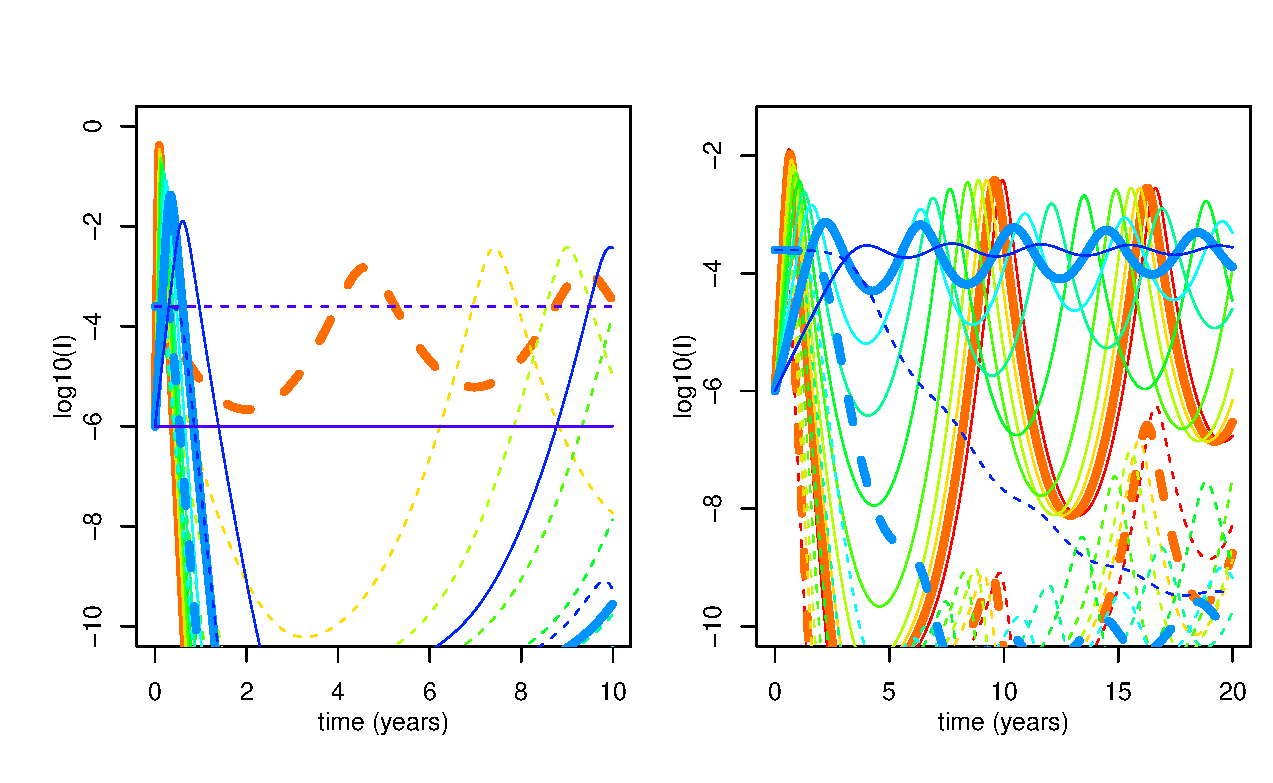
\includegraphics[width=0.9\linewidth]{gupta.eps}
%  \caption{}
%\label{fig:traj_siri2}
%\end{figure}
%
%\clearpage


%%% Local Variables: 
%%% mode: latex
%%% TeX-master: "../../phD"
%%% End: 

%\cleardoublepage
%\newpage
%\newpage
%\thispagestyle{empty}
%\mbox{}

\clearpage
\newpage
\thispagestyle{empty}
\null
\newpage


\input{texte/article2/appendix_eliza.tex}
%\newpage
%\thispagestyle{empty}
%\mbox{}
\clearpage
\newpage
\thispagestyle{empty}
\null
\newpage


\chapter{Supporting Information: The transition from invasion to
  persistence for influenza antigenic units}


%\title{Introducing gradual antigenic drift in co-circulating
%  cross-reactive antigenic clusters models}

%other title proposals
%\title{Chaotic dynamics with uniform phase in influenza
%  epidemics: from theory to observation}


Sébastien Ballesteros$^{1,*}$,
Anton Camacho$^{1}$,
Elisabeta Vergu$^{2}$,
Bernard Cazelles$^{1,3}$

\tikzstyle{naif} = [draw, fill=white, rectangle, minimum height=2em, minimum width=3em]
\tikzstyle{expo} = [draw, fill=blue, circle,minimum height=2em]
\tikzstyle{mut} = [draw, fill=red, circle,minimum height=2em]

\definecolor{monVert}{RGB}{120,212,144}
\tikzstyle{class_X} = [draw, fill=blue!20, rectangle, minimum height=2em, minimum width=3em]
\tikzstyle{class_X_2} = [draw, fill=monVert, rectangle, minimum height=2em, minimum width=3em]
\tikzstyle{class_X_3} = [draw, fill=red!20, rectangle, minimum height=2em, minimum width=3em]

\tikzstyle{class_I} = [draw, fill=blue!20, circle,minimum height=2em]
\tikzstyle{class_I_2} = [draw, fill=monVert, circle,minimum height=2em]



\vspace{2cm}

$^1$UMR 7625  (UPMC, ENS, AgroParisTech, CNRS), Ecole Normale Supérieure, Unit of Eco-Evolutionary Mathematics,  46 rue d'Ulm, F-75230 Paris Cedex 05, France. \\
$^2$~INRA, UR341 Mathématiques et Informatique Appliquées, F-78352 Jouy en Josas, France \\
$^3$~IRD UR GEODES, 93142 Bondy, France

~\\
$^*$\textit{Corresponding author}:  \\
E-mail: sebastien.ballesteros@biologie.ens.fr



\section{Justification of the $SIRX$ model}

Here we justify the use of the two levels $SIRX$ model.  We first
introduce single level history based model, and then consider status
based model as the choice of a given framework can have important
consequences on both transient \citep{Ballesteros2009} and stationary
\citep{Dawes2002} dynamics.

\subsection{History based models}

Using the $SIRS$ description of antigenic drift \citep{Pease1987}, we
can incorporate gradual antigenic drift into a two IAU model starting
from simple two strains $SIR$ models and adding loss of immunity
induced by viral evolution (figure~\ref{fig:drawbacks}).

\begin{figure}[h!]
  \center
%%%%%%%%%%%%%%%%%%%%%%%%%%%%%%%%%%%%%%%%%%%%%%%%%%%%%%%%%%%%%%%%%%%%%%%%%
% naive status based model (reduced susceptibility)
%%%%%%%%%%%%%%%%%%%%%%%%%%%%%%%%%%%%%%%%%%%%%%%%%%%%%%%%%%%%%%%%%%%%%%%%%
\begin{minipage}{0.45\linewidth}
  \begin{tikzpicture}[node distance=1.4cm, inner sep=0pt, minimum size=8mm]
    \tikzstyle{seb}=[rectangle, fill=red, draw=gray, text=black]
    \tikzstyle{I1}=[->, draw=red, shorten >=1pt, >=stealth',semithick]
    \tikzstyle{I2}=[->,draw=blue, shorten >=1pt, >=stealth',semithick]
    \tikzstyle{g1}=[->,shorten >=1pt, >=stealth',semithick]
    \tikzstyle{g2}=[->,shorten >=1pt, >=stealth',semithick]

    \node[seb] (R0) {$R_\varnothing$};
    \node[seb] (R1) [above of=R0] {$R_1$};
    \node[seb] (R2) [below of=R0] {$R_2$};
    \node[seb] (R12) [right of=R0] {$R_{12}$};

    \draw[I1] (R0) to node[auto] {\begin{tiny}$(1-\sigma'_{12}) \beta R_\varnothing I^1$\end{tiny}} (R1);
    \draw[I2] (R0) to node[auto,swap] {\begin{tiny}$(1-\sigma'_{12}) \beta R_\varnothing I^2$\end{tiny}} (R2);
    \draw[I2] ([yshift=+4mm] R1.east) to node[auto] {\begin{tiny}$\beta R_1 I^2$\end{tiny}} ([yshift=+4mm] R12.west);
    \draw[I1] ([yshift=-4mm] R2.east) to node[auto,swap] {\begin{tiny}$\beta R_2 I^1$\end{tiny}} ([yshift=-4mm] R12.west);
    \draw[g1] ([xshift=+2mm] R1.south) to node[auto] {\begin{tiny}$\gamma_1 \gamma_2$\end{tiny}} ([xshift=+2mm] R0.north);
    \draw[g2] ([xshift=+2mm] R2.north) to node[auto,swap] {\begin{tiny}$\gamma_2 \gamma_1$\end{tiny}} ([xshift=+2mm] R0.south);
    \draw[g1] (R12.west) to (R2.east) ;
    \draw[g2] (R12.west) to (R1.east) ;
    \draw[I1] ([yshift=+1mm] R0.east) to node[auto] {\begin{tiny}$\sigma'_{12} \beta R_\varnothing I^1$\end{tiny}} ([yshift=+1mm] R12.west);
    \draw[I2] ([yshift=-1mm] R0.east) to node[auto,swap] {\begin{tiny}$\sigma'_{12} \beta R_\varnothing I^2$\end{tiny}} ([yshift=-1mm] R12.west);
\end{tikzpicture}
\end{minipage}
%%%%%%%%%%%%%%%%%%%%%%%%%%%%%%%%%%%%%%%%%%%%%%%%%%%%%%%%%%%%%%%%%%%%%%%%%
% naive history based model (reduced susceptibility)
%%%%%%%%%%%%%%%%%%%%%%%%%%%%%%%%%%%%%%%%%%%%%%%%%%%%%%%%%%%%%%%%%%%%%%%%%
\begin{minipage}{0.45\linewidth}
  \begin{tikzpicture}[node distance=1.4cm, inner sep=0pt, minimum size=8mm]
    \tikzstyle{seb}=[rectangle, fill=red, draw=gray, text=black]
    \tikzstyle{I1}=[->, draw=red, shorten >=1pt, >=stealth',semithick]
    \tikzstyle{I2}=[->,draw=blue, shorten >=1pt, >=stealth',semithick]
    \tikzstyle{g1}=[->,shorten >=1pt, >=stealth',semithick]
    \tikzstyle{g2}=[->,shorten >=1pt, >=stealth',semithick]

    \node[seb] (R0) {$R_\varnothing$}; 
    \node[seb] (R1) [above of=R0] {$R_1$};
    \node[seb] (R2) [below of=R0] {$R_2$};
    \node[seb] (R12) [right of=R0] {$R_{12}$};

    \draw[I1] (R0) to node[auto] {\begin{tiny}$\beta R_\varnothing I^1$\end{tiny}} (R1);
    \draw[I2] (R0) to node[auto,swap] {\begin{tiny}$\beta R_\varnothing I^2$\end{tiny}} (R2);
    \draw[I2] ([yshift=+4mm] R1.east) to node[auto] {\begin{tiny}$\sigma_{12} \beta R_1 I^2$\end{tiny}} ([yshift=+4mm] R12.west); 
    \draw[I1] ([yshift=-4mm] R2.east) to node[auto,swap] {\begin{tiny}$\sigma_{12} \beta R_2 I^1$\end{tiny}} ([yshift=-4mm] R12.west);
    \draw[g1] ([xshift=+2mm] R1.south) to node[auto] {\begin{tiny}$\gamma_1 \gamma_2$\end{tiny}} ([xshift=+2mm] R0.north); 
    \draw[g2] ([xshift=+2mm] R2.north) to node[auto,swap] {\begin{tiny}$\gamma_2 \gamma_1$\end{tiny}} ([xshift=+2mm] R0.south) ;
    \draw[g1] (R12.west) to (R2.east) ;
    \draw[g2] (R12.west) to (R1.east) ;
  \end{tikzpicture}
\end{minipage}
\caption{Drawbacks of introducing antigenic drift in simple status
  based (left) and history based (right) two strains (here IAU) models
  (reduced susceptibility assumption). Red (blue) arrows represent
  infection by IAU 1 (2). Black arrows represent within IAU antigenic
  evolution.}
\label{fig:drawbacks}
\end{figure}

In a history based model with reduced susceptibility
(figure~\ref{fig:drawbacks}, right ; eq~\eqref{eq:appendix3:HBRS}),
infection of hosts naive to both IAU $i$ and $j$ ($R_\varnothing$)
with IAU $i$ results in all infected hosts acquiring immunity to $i$
($R_\varnothing \rightarrow R_i$) and a partial protection to $j$ that
will be determined at the encounter time with $j$. As IAU $i$ evolves,
the population looses immunity to IAU $i$.

This processes can be formalised by extending multi strain model of
\cite{Andreasen1997} to include gradual antigenic drift within IAU
(eq~\eqref{eq:appendix3:HBRS}) (note that we also allow coinfections)

%HBRS 1 level coinfections
\begin{align}
  \label{eq:appendix3:HBRS}
  \dot{R_\varnothing} &= \mu N -\sum_k \beta_k R_\varnothing \frac{I^k}{N} +\sum_{k \in K} g_k
  R_k - \mu R_\varnothing\\
  %% 
  \dot{R_J} &= \sum_{k \in J} \beta_k {\sigma}^k_{J \setminus k} R_{J
    \setminus k} \frac{I^k}{N} - \sum_{k \notin J} \beta_k {\sigma}^k_J R_J \frac{I^k}{N} -
  \sum_{k \in J} g_k R_J + \sum_{k \notin J} g_k
  R_{J \cup k} -\mu R_J \notag \\
  %% 
  \dot{I^k} &= \sum_{J \subseteq \{K \setminus k\}} {\sigma}^k_J \beta_k
  R_J \frac{I^k}{N} -\nu I^k -\mu I^k \notag
\end{align}

where $J$ denotes the set of all previous IAU (belonging to the set
$K$) that have successfully infected and immunised the hosts.

At the single IAU level, model of eq \eqref{eq:appendix3:HBRS} is
reduced to the classical $SIRS$ model. The addition of gradual
antigenic drift increases the proportion of infectious hosts at the
endemic equilibrium compared to the $SIR$ model resulting in:
$I_{SIRS}^*=\frac{e+\gamma}{1+\gamma} (1-\frac{1}{r}) =I_{SIR}^* +
\frac{\gamma}{1+\gamma}R_{SIR}^*$. The number of susceptible
individuals ($R_\varnothing$) however remains the same as for the
$SIR$ model with an equilibrium value of $1/r$.  In the absence of
functional constraints, this condition renders the invasion of a
second IAU always possible in a population where a resident IAU is at
the endemic equilibrium.


One of the major drawbacks of the multi IAU $SIRS$ model ($muSIRS$) is
that if IAU $i$ evolves we loose the fact that $R_i$ hosts (now
$R_\varnothing$) are partially protected to the second IAU. This
assumption would be relevant for waning immunity but in our case
contradicts the fact that influenza specific immune response appears
to be long-lived. The memory of partial protection is important to
take into account as the IAU can be considered separated by a fixed
antigenic distance that remains constant despite within IAU evolution
\citep{Blackburne2008}. Only punctual events create new IAU.


Keeping track of partial cross protection despite within IAU gradual
antigenic drift is possible by introducing a new compartment $X$
(figure \ref{fig:sirx}).

\begin{figure}[H]
\center
  \begin{tikzpicture}[node distance=2cm, auto,>=latex', thick]
    \tikzstyle{seb}=[->,draw=red, shorten >=1pt, >=stealth',semithick]
    % We need to set at bounding box first. Otherwise the diagram
    % will change position for each frame.
    % \path[use as bounding box] (-1,0) rectangle (10,-2);
    \node [naif] (S) {$S$};
    \node [expo, right of=S] (I) {$I$};
    \node [expo, right of=I] (R) {$R$};
    \node [expo, right of=R] (X) {$X$};
    \node [mut, below of=I] (I2) {$I_2$};
    % \node [mut, below of=R] (I2) {$I_2$};
    % \node [mut, below of=X] (I2) {$I_2$};
    
    % Once the nodes are placed, connecting them is easy. 
    \draw [->] (S) -- node {$r$} (I);
    \draw [->] (I) -- node{$(1-e)$}(R);
    \draw [->] (R) -- node{$\gamma$}(X);
    \draw[seb, ->](X) -- +(0,1) -| node[near start,above] {$\sigma_X r$} (I);
    \draw [->] (S) -- node {$\alpha r$} (I2);
    \draw [->] (I) -- node {$\sigma_{12} \alpha r$} (I2);
    \draw [->] (R) -- node {$\sigma_{12} \alpha r$} (I2);
    \draw [seb, ->] (X) -- node {$\sigma_{12} \alpha r$} (I2);    
  \end{tikzpicture}
  \caption{The $SIRX$ model: new-borne ($S$) have full susceptibility,
    within IAU antigenic evolution results in the loss of full
    immunity toward strain of the IAU ($R \to X$). $X$ host can
    retain a level of partial protection to reinfection
    ($\sigma_X$). Hetero unit partial protection is ensured by
    parameter $\sigma_{12}$.}
\label{fig:sirx}
\end{figure}

This is the model used in main text.

Keeping track of partial protection despite within IAU antigenic
evolution have important consequences on the invasion condition of a
mutant IAU. Here we generalise the invasion threshold presented in
main text to a population where $K$ identical unrelated (and therefore
non cross reactive) resident IAU are at the endemic equilibrium. This
condition can be calculated with
 $$\left. \frac{d I^{K+1}}{d t} \right|_{1^*,\dots, K^*} =
(r_{K+1} R_{\begin{subarray}{l}\varnothing \\
    \varnothing \end{subarray}}^* + \sigma_{12} r_{K+1}
(1-R_{\begin{subarray}{l}\varnothing \\ \varnothing \end{subarray}}^*)
-1) I^{K+1}$$
where we use non dimensional form of the models by
rescaling natural time $t$ in unit of duration of infection and note
$r=\frac{\beta}{\mu+\nu}$, $e=\frac{\mu}{\mu+\nu}$;
$\gamma=\frac{g}{\mu+\nu}$.

In the following, we assume that $r_{K+1}=\alpha r$ and expect $\alpha
\leq 1$ due to functional constraints.

The invasion condition can be expressed as $\sigma_{12} > \frac{1-\alpha
  r R_{\begin{subarray}{l}\varnothing \\
      \varnothing \end{subarray}}^*}{\alpha
  r(1-R_{\begin{subarray}{l}\varnothing \\
      \varnothing \end{subarray}}^*)}$ and is determined only by
$R_{\begin{subarray}{l}\varnothing \\ \varnothing \end{subarray}}^*$


This expression is also valid for the $muSIRS$ model. For this latter
model, when $K=1$, the number of fully naive hosts is given by
$1/r$. In the absence of functional constraints ($\alpha=1$) fully
naive hosts are always in a sufficient number to ensure the invasion
of a mutant IAU ($1-r R_{\begin{subarray}{l}\varnothing \\
    \varnothing \end{subarray}}^*=0$) and there is no invasion
threshold.  Situation changes with the $SIRX$ model or when $K>1$
unrelated IAU co-circulate. In these cases,
$R_{\begin{subarray}{l}\varnothing \\ \varnothing \end{subarray}}^*$
can be calculated from: $\frac{dR_{\begin{subarray}{l}\varnothing \\
      \varnothing \end{subarray}}^*}{dt} = 0 = e -r
R_{\begin{subarray}{l}\varnothing \\ \varnothing \end{subarray}}
\sum_kI^k -e
R_{\begin{subarray}{l}\varnothing \\ \varnothing \end{subarray}}$.\\

As there is no competition at all in the resident population, the
endemic equilibrium of IAU $k \in [1,\dots,K]$, ${I^k}^*$ are all
identical to the value $I^*$ of the single IAU model.  The invasion
condition can then be expressed as a function of $I^*$:
$\sigma_{12}>\frac{KrI^*+e(1-\alpha r)}{K \alpha r^2 I^*}$.  In the
special cases where $\sigma_X=1$ an exact expression can be derived as
$I^*$ is given by the equilibrium of the simple $SIRS$ model.

\begin{align}
  \label{eq:appendix3:threshold}
  \sigma_{12} &> \frac{1}{\alpha r} - \frac{e(1+\gamma)(\alpha r-1)}{K
    \alpha r (e+\gamma)(r-1)}
\end{align}

In this latter case, gradual antigenic drift within IAU $g>0$ ensures
an invasion threshold even when $K=1$ and $\alpha=1$.  and possesses
an upper bound $=\frac{1}{r} - \frac{e}{K r}$ as $\gamma \to \infty$.

As we show in main text, the invasion of a mutant IAU is always
possible whenever $\sigma_{12} > \sigma_X$.

This sufficient condition is not limited to the simple $SIRX$ model
and remains valid for models allowing a flexible shape of the
evolution of the reinfection probability following antigenic drift
such the one used by \citet{Xia2005}.


The model depicted in figure~\ref{fig:general} allow to consider
flexible shape of the evolution of the reinfection probability
following antigenic drift.  Note that as hosts never come back to the
$S$ compartment, we ensure that hosts partially protected to a new IAU
keep their partial protection even if the originally immunising IAU is
subject to antigenic drift rendering reinfection by the same IAU
possible.  The flexibility of this model was used by \cite{Xia2005} to
infer the shape of the immunity decay following influenza infection.
$(1-\sigma_{12})$ is the reduction of susceptibility due to inter-IAU
partial cross protection and $(1-\sigma_X)$ is the the reduction of
susceptibility due to within-IAU partial cross protection.

\begin{figure}[h!]
\center
\begin{tikzpicture}[node distance=2cm, auto,>=latex', thick]
  \tikzstyle{seb}=[->,draw=red, shorten >=1pt, >=stealth',semithick]
    % We need to set at bounding box first. Otherwise the diagram
    % will change position for each frame.
%    \path[use as bounding box] (-1,0) rectangle (10,-2);
    \node [naif] (S) {$S$};
    \node [expo, right of=S] (I) {$I$};
    \node [expo, right of=I] (R1) {$R_1$};
    \node [expo, right of=R1] (R2) {$R_2$};
    \node [expo, right of=R2] (Rk) {$R_K$};
    \node [mut, below of=I] (I2) {$I_2$};

% Once the nodes are placed, connecting them is easy. 
    \draw [->] (S) -- node {$r$} (I);
    \draw [->] (I) -- node{$(1-e)$}(R1);
    \draw [->] (R1) -- node{$K \gamma$}(R2);
    \draw [->] (R2) -- node{...}(Rk);
    \draw[->](R1) -- +(0,1) -| node[near start,above] {$\sigma_X^1 r$}
    (I);
    \draw[->](R2) -- +(0,1.7) -| node[near start,above] {$\sigma_X^2 r$}
    (I);
    \draw[->](Rk) -- +(0,2.4) -| node[near start,above] {$\sigma_X^K r$}
    (I);

    \draw [seb, ->] (S) -- node {$\alpha r$} (I2);
    \draw [seb, ->] (I) -- node {$\sigma_{12} \alpha r$} (I2);
    \draw [seb, ->] (R1) -- node {$\sigma^1_{12} \alpha r$} (I2);
    \draw [seb, ->] (R2) -- node {$\sigma^2_{12} \alpha r$} (I2);
    \draw [seb, ->] (Rk) -- node {$\sigma^K_{12} \alpha r$} (I2);
    
\end{tikzpicture}
\caption{A general model for a drifting antigenic unit.}
\label{fig:general}
\end{figure}

Using figure~\ref{fig:general} model, the invasion condition of a
second IAU can be calculated with:\\
$\left. \frac{d I^2}{d t} \right|_{1^*} = (\alpha r S^* + \alpha r (
\sum_k \sigma^k_{12} R_k^* + \sigma_{12} I) -1) I^2 >0$.

Assuming that the first IAU is at the epidemiological equilibrium
ensures that: $\frac{dI}{dt} = r S I +r \sum_k \sigma_X^k R_k I -I = 0
\Rightarrow r S^* + r \sum_k \sigma_X^k R_k^*=1$

Considering $\alpha=1$, invasion is always possible if $\sum_k
\sigma^k_{12} R_k^* > \sum_k \sigma_X^k R_k^*$. This condition is always
true if $\forall{k} \in [1, ..., K]$, $\sigma^k_{12} > \sigma_X^k$. Note
that in the absence of co-infections, this condition also defines the
invasion threshold.

$\sigma^k_{12} > \sigma_X^k$, $\forall{k} \in [1, ..., K]$, therefore
constitutes a sufficient condition for the invasion of the mutant
IAU.





\subsection{Status based model}


%SBRI---------------

Within a status based framework (figure~\ref{fig:drawbacks}, left),
following infection with IAU $i$, naive hosts acquire immunity to $i$
($R_i$) and a given proportion ($\sigma'_{12}=1-\sigma_{12}$) acquires
immunity to both $i$ and $j$ ($R_{ij}$) and are therefore no more
susceptible for both IAUs $i$ and $j$ (polarized immunity
\citet{Gog2002a}).  We can thus easily take into account the fact that
IAU $i$ can evolve and thus the population looses immunity to cluster
$i$ but not to cluster $j$. This results in a $R_{ij} \rightarrow R_j$
transfer.

Contrary to history based model, assuming that cross-immunity acts by
reducing susceptibility or infectivity have strong consequecences on
status based model \citep{Ballesteros2009}.  All the theoretical
studies supporting the punctuated theory of influenza immune escape
have used the reduced infectivity formalism ($SBRI$ model) as it
results in comparatively low dimensional models.  The $SBRI$ model
including within IAU gradual antigenic drift is depicted in
eq~\eqref{eq:SBRI} where $S_k$ denotes hosts susceptible to IAU $k$.

%SBRI
\begin{footnotesize}
  \begin{align}
    \label{eq:SBRI}
    \dot{S_k} &= \mu N -\sum_j \beta_j(t) {\sigma'}_{kj} S_k
    \frac{I^j}{N}
    - \mu S_k +g_k (N-S_k-I^k)\\
  %% 
    \dot{I^k} &= \beta_k S_k \frac{I^k}{N} -\nu I^k -\mu I^k \notag
  \end{align}
\end{footnotesize}

In case of reduced susceptibility assumption ($SBRS$ model), including
within IAU gradual antigenic drift results in eq~\eqref{eq:SBRS}.

\begin{footnotesize}
  \begin{align}
    \label{eq:SBRS}
    \dot{R_\varnothing} &= \mu N -\sum_k \beta_k R_\varnothing
    \frac{I^k}{N} +\sum_{k \in K} g_k
    R_k - \mu R_\varnothing\\
  %% 
    \dot{R_J} &= \sum_{k, L \subseteq K} C(L,J,k) \beta_k
    \frac{I^k}{N} R_L -\sum_{k \in \{J \setminus k\}} \beta_k
    \frac{I^k}{N} R_J -\sum_{k \in J} g_k R_J + \sum_{k \notin J} g_k
    R_{J \cup k} -\mu R_J \notag \\
  %% 
    \dot{I^k} &= \sum_{J \subseteq \{K \setminus k\}} \beta_k R_J
    \frac{I^k}{N} -\nu I^k -\mu I^k \notag
  \end{align}
\end{footnotesize}

where following \citet{Gog2002a}, 

$$C(L,J,k)=
\begin{cases}
  \prod_{j \in J \setminus L} \sigma'_{kj} \prod_{j \notin J}
  (1-\sigma'_{kj}) & \text{if } k \notin L \text{ and } L \subset J \\
  0 & \text{otherwise.}
\end{cases}$$


As shown in figure \ref{SBRI_2}, the status-based formulation induces
an immune boosting dynamics that can be illustrated in the 2-IAUs
case. When IAU $2$ has yet not appeared and thus does not evolve (no
gradual antigenic drift for $2$), figure \ref{SBRI_2} shows that, in
the absence of birth, $R_{2}+R_{12}$ form an absorbing class. The
infection dynamics of strain $1$ rapidly results in an equilibrium
mostly governed by a reinfection dynamics between $R_2$ and
$R_{12}$. This process results in the fact that when cluster $2$
appears, it cannot invade as all the hosts have full immunity to
$2$. Moreover, with the assumption of reduced infectivity, the $SBRI$
model leads to a transfer $R_{1}\to R_{12}$ (in red on figure
\ref{SBRI_2}) that overestimates the immunity against IAU 2. From a
biological stand point, this additional transfer resulting from
reinfection of $R_1$ by IAU 1 is even more problematic as it is in
disagreement with the original antigenic sin mechanism
\citep{Ballesteros2009}.

\begin{center}
\begin{figure}[h!]
\centering
\begin{tikzpicture}[node distance=3cm, auto,>=latex', thick]

  \tikzstyle{output} = [coordinate]
  
  \node [class_X] (R0) {$R_{\emptyset}$};	
  
  \node [class_X_3, right of=R0,node distance=5cm] (R12) {$R_{12}$};
  
  \draw [->] (R0) --node[name=R0R12] {$\sigma'_{12}\lambda_1$}(R12);
  
  \node [class_X_2, above of=R0R12,node distance=2cm] (R1) {$R_1$};
  \node [class_X_2, below of=R0R12,node distance=2.5cm] (R2) {$R_2$};
  
  \draw [->] (R0) edge[bend left]node[left]{$(1-\sigma'_{12})\lambda_1$}(R1);
  \draw [->] (R1) edge[bend left]node[above]{$g_{1}$}(R0);
  
  \draw [->] (R1) edge[bend left]node[right]{$\textcolor{red}{\sigma'_{12}\lambda_1}$}(R12);
  
  \draw [->] (R2) edge[bend right]node[right]{$\lambda_1$}(R12);
  \draw [->] (R12) edge[bend right]node[below]{$g_{1}$}(R2);
  
\end{tikzpicture}
\caption{Schematic representation of the immune boosting induced by
  status-based frameworks. The assumption of reduced infectivity leads
  to an additional transfer $R_{1}\to R_{12}$ (in red). $\lambda_{1}$
  is the infection force of IAU 1. Note that for comparison purpose
  with history based model, the cross-immunity intensity
  $\sigma'_{12}$ can be simply related to the immune escape intensity
  by $\sigma_{12}=1-\sigma'_{12}$.}
\label{SBRI_2}
\end{figure}
\end{center}

\clearpage

More quantitatively, the impeded invasion produced by the status based
framework can be determined by standard invasion analysis. For
instance for the $SBRI$ model of eq.\eqref{eq:SBRI}, the invasion
condition can be calculated by:

\begin{align}
  \left. \frac{d I^2}{d t} \right|_{S_2^*} & =
  (r_2 S_2^* -1) I^2 \label{eq:invasion_sbri}
\end{align}

where $S_2^*$ is determined by the equilibrium of the 2-IAU model with
$I^2=0$.

Invasion of the mutant IAU implies $\left. \frac{d I^2}{d t}
\right|_{S_2^*} \geq 0$ and results in a threshold on $\sigma'_{12}$:
 $$\sigma'_{12} \leq \frac{(r_2-1)(e+\gamma_2)(1+\gamma_1)}{(r_1-1)(e+\gamma_1)}$$.  
 In the following we assume $r_2=r_1$ ($\alpha=1$ no functional
 constraints). If $\gamma_2=0$ until IAU 2 appears there is an
 invasion trheshold. This threshold does not depend on $R_0$ (here,
 $r$) and is represented on figure~\ref{fig:threshold_koelle}. Note
 however that if $\gamma_2=\gamma_1$ before IAU 2 emerges the invasion
 condition is always satisfied.

\begin{figure}[!htbp]
  \center
  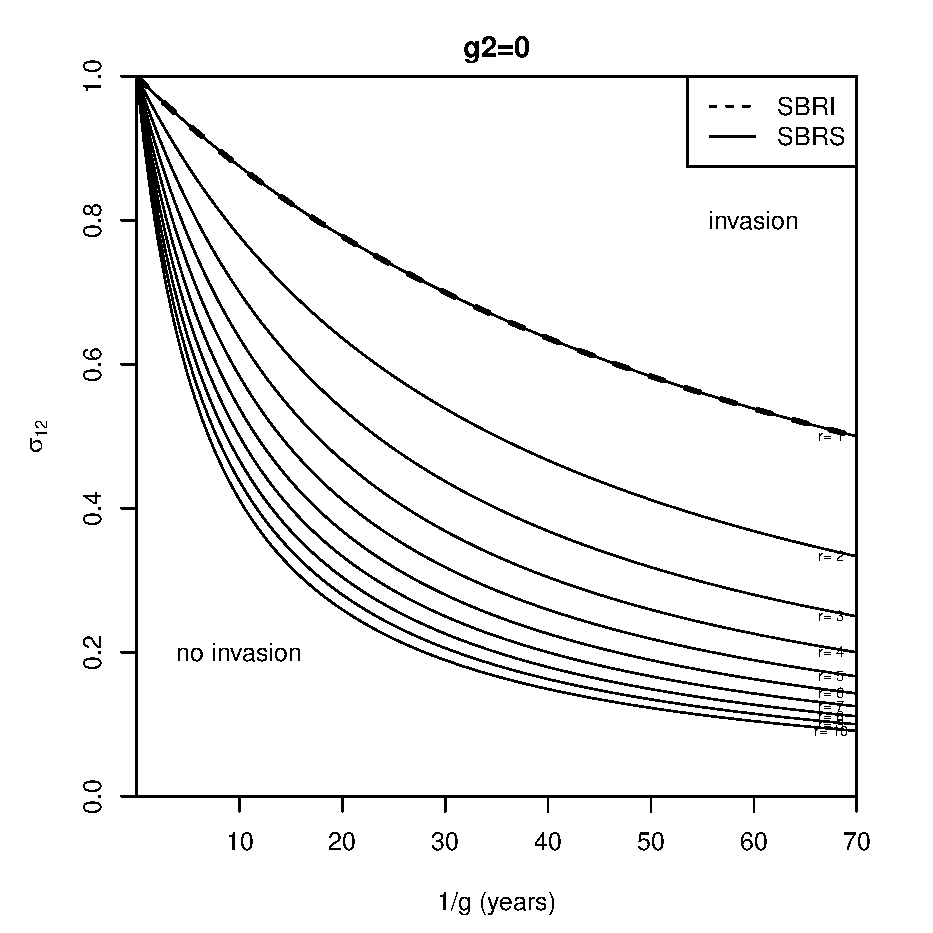
\includegraphics[width=0.3\linewidth]{texte/article3/appendix_diamond/graph/threshold_koelle.eps}
  \caption{Invasion threshold for the two antigenic unit status based
    model ($SBRI$ and $SBRS$) with $r_2=r_1$. Note that for comparison
    purpose with history based model, the y-axis is expressed in
    immune escape intensity with $\sigma_{12}=1-\sigma'_{12}$.}
  \label{fig:threshold_koelle}
\end{figure}

The same results can be established for the $SBRS$ model. The
threshold is given by:
$$\sigma'_{12} \leq \frac{r_1 (r_2-1) (e+\gamma_2)
  (\gamma_2 +r_1(e+\gamma_1)}{(r_1-1)(e+\gamma_1) (\gamma_1 r_1
  +r_2(\gamma_2+e r_1))}$$ and plotted on
figure~\ref{fig:threshold_koelle}.  This threshold depends on $r_{1/2}$
and equal the one of the $SBRI$ model when $r_{1}=r_{2}=1$.

Considering $\gamma_2=\gamma_1$ means that IAUs may evolve
before they have emerged. This hypothesis could be supported if
IAUs co-circulate in a region outside the population area and are
introduced following a source-sink process. However, in the context
of influenza antigenic clusters giving rise to each others, we do not find any biological
motivation.  When $\gamma_2=\gamma_1$, the $SBRS$ model also ensures
invasion of the mutant IAU even if $\sigma_{12}=0$ rendering
immune escape difficult to interpret.

Introducing within IAU gradual antigenic drift in status based
multi-strains models can therefore result in an invasion threshold for
a second IAU. As the same model without gradual antigenic
drift does not present this threshold property \citep{Ballesteros2009},
the impeded invasion comes from the immune boosting dynamics
previously described. Due to this immune boosting dynamics, the timing
of introduction of successive IAUs is of tremendous importance
: if the resident IAU has circulated sufficiently long to
fill in compartments $R_2$ and $R_{12}$ then gradual
antigenic drift will result in a strong invasion threshold for the
next IAU. In contrast, if the mutant IAU appears
sufficiently soon, it will be able to invade. 

\subsection{Comparison of status based and history based framework:
  effect of cross-immune boosting}

In order to examine the influence of the cross-immune boosting
dynamics previously described on the outcome of IAU invasion we
contrast the widely used $SBRI$ model with an equivalent history based
model.  Due to the hypothesis of polarised immunity, the inclusion of
within IAU gradual antigenic drift into status based model results in
full susceptibility of the hosts to within IAU reinfection but do not
cancel partial cross protection against other IAUs.  This assumption
can be translated in the $SIRX$ framework by taking its $SIRS$ limit
($\sigma_{X}=1$) \textit{i.e.} by taking the following matrix of
susceptibility reduction: $\mathbf{\sigma_H^k} = \bordermatrix{ & 1 &
  2\cr 1 & 1 & \sigma_{12} \cr 2 & \sigma_{12} & 1 \cr 12 & 1 & 1 \cr
}$. Contrary to the status based model, the equivalent history based
model does not result in cross immune boosting dynamics whereas both
models reduce to the $SIRS$ model at the single IAU level.

In order to simplify the analysis we will consider the invasion of an
IAU already established and subject to gradual antigenic drift in a
source population but not in our focal population \textit{i.e.}
$g_{1}=g_{2}$. This assumption will ensure equality of mutant and
resident antigenic drift rate and therefore cancel the need to study
the effect of the introduction time of the mutant for the status based
model.

\begin{figure}[!htbp]
  \center
  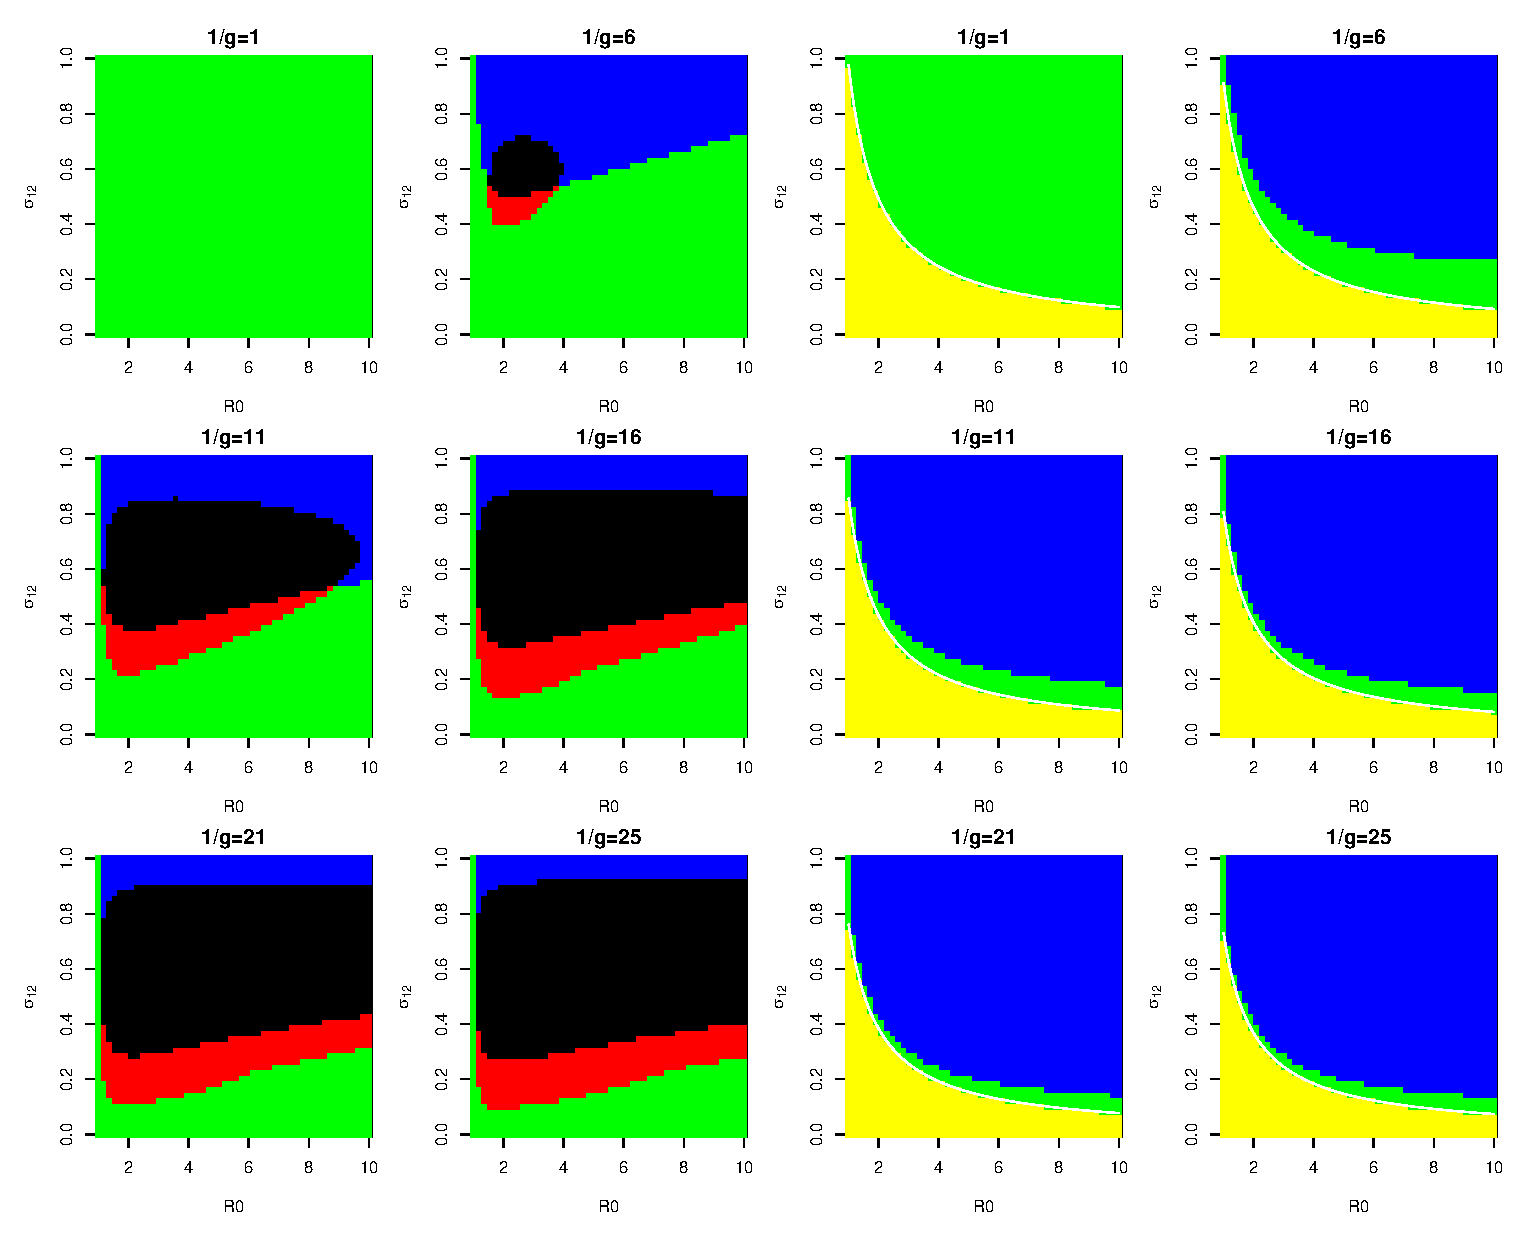
\includegraphics[width=0.8\linewidth]{texte/article3/appendix_diamond/graph/koelle_vs_purely_transiant.eps}
  \caption{Outcomes of the transient invasion dynamics of a new
    IAU within a population where a resident IAU
    is at the endemic equilibrium. First and second column figures are for
    the $SBRI$ model generalised to include within IAU
    gradual antigenic drift (with $g_2=g_1$) ; third and fourth
    column figures are for the equivalent history based model. Colours: both
    IAUs go extinct (black), the resident IAU only goes
    extinct (successful replacement, red); the mutant IAU only goes
    extinct (blue); no IAU goes extinct (coexistence, green); the
    mutant IAU cannot invade (yellow). White curve is the invasion
    threshold given by eq.~\eqref{eq:appendix3:threshold}. As a deterministic
    model is used, extinctions are determined by a threshold value of
    $1.10^{-9}.$}
  \label{fig:koelle_vs}
\end{figure}

As it can be seen in figure~\ref{fig:koelle_vs}, the $SBRI$ model has
a tremendous impact on the outcome of the transient dynamics of
drifting IAUs replacement. Within an equivalent model stated within
the $SIRX$ framework, no replacement (red areas in
figure~\ref{fig:koelle_vs}) are possible for parameter values
compatible with influenza. In place of replacement, the $SIRX$ model
gives rise to a sharp transition from coexistence (green areas in
figure~\ref{fig:koelle_vs}) to self extinction without replacement
(blue areas in figure~\ref{fig:koelle_vs}).



\section{Reinfection limits}

The number of compartment (scaling in $3^{N_K}$) of the $SIRX$, the
$SIRXQ1$ and the $SIRXQ12$ with immune boosting model can be reduced
to $2^{N_K}$ by taking the limit $g \to \infty$.

In case of the $SIRX$ model the reinfection limit leads to
\eqref{eq:SIRI}.

\begin{align}
  \label{eq:SIRI}
  \dot{R_\varnothing} &= \mu N -\sum_k \beta_k R_\varnothing \frac{I^k}{N} - \mu R_\varnothing\\
  %% 
  \dot{R_J} &= \sum_{k \in J} \beta_k \sigma^k_{J \setminus k} R_{J
    \setminus k} \frac{I^k}{N} - \sum_{k \notin J} \beta_k \sigma^k_J R_J \frac{I^k}{N} -\mu R_J \notag \\
  %% 
  \dot{I^k} &= \sum_{J \subseteq K} \sigma^k_J \beta_k
  R_J \frac{I^k}{N} -\nu I^k -\mu I^k \notag
\end{align}

This model is comparable to \cite{Goekaydin2007} model with the
difference that \eqref{eq:SIRI} model allows for coinfections.

Taking the limit $g \to \infty$ of the $SIRXQ1/12$ model results in:

\begin{align}
  \label{eq:SIRIQ}
  \dot{R_\varnothing} &= \mu N -\sum_k \beta_k R_\varnothing \frac{I^k}{N} - \mu R_\varnothing\\
  %% 
  \dot{I^k_J} &= \sigma^k_J \beta_k
  R_J \frac{I^k}{N} + \sigma^k_{J \setminus k} \beta_k
  R_{J \setminus k} \frac{I^k}{N} -\nu I^k_J -\mu I^k_J \notag \\
  %% 
  \dot{Q_J} &= \sum_{k \in J} \nu I^k_J -q Q_J -\mu Q_J \notag \\
  %%
  \dot{R_J} &=  q Q_J - \sum_{k} \beta_k \sigma^k_J R_J \frac{I^k}{N} -\mu R_J \notag
\end{align}

in the absence of immune boosting ($SIRXQ1$) and:

\begin{align}
  \label{eq:SIRIQferg}
  \dot{R_\varnothing} &= \mu N -\sum_k \beta_k R_\varnothing \frac{I^k}{N} - \mu R_\varnothing\\
  %% 
  \dot{I^k_J} &= \sigma^k_J \beta_k
  R_J \frac{I^k}{N} + \sigma^k_{J \setminus k} \beta_k
  R_{J \setminus k} \frac{I^k}{N} -\nu I^k_J -\mu I^k_J \notag \\
  %% 
  \dot{Q_J} &= \sum_{k \in J} \nu I^k_J -q Q_J -\mu Q_J \notag \\
  %%
  \dot{R_J} &=  q Q_J + q Q'_J -\sum_{k} \beta_k R_J \frac{I^k}{N} -\mu R_J \notag \\
  %% 
  \dot{Q'^k_J} &= \sum_{k} (1 - \sigma^k_J) \beta_k R_J \frac{I^k}{N}  -q Q'_J -\mu Q'_J \notag
\end{align}

with immune boosting ($SIRXQ12$).

\section{Additional figures}

\subsection{Transient dynamics: determinist models}

\begin{figure}[!hp]
  \center
  \includegraphics[width=0.9\linewidth]{texte/article3/appendix_diamond/graph/traj_deter.eps}
  \caption{Transient invasion dynamics of a mutant antigenic unit in a
    population where a resident antigenic unit is at its endemic
    equilibrium. Red and blue are prevalence of mutant and resident
    antigenic unit in log scale. Colours intensity indicates the
    degree of immune escape as measured by $\Delta\sigma$ (1\%
    (light tones); 5\%, 10\%, 20\% and 30\% (dark tones)). Parameters:
    $R_0=2$; $1/\nu=4$ days ; $1/g=1$ year ; $1/q=6$
    months. Figure~\ref{fig:traj_deter_reinfection} reveals the
    dynamics obtain by taking the limit $g \to \infty$}
  \label{fig:traj_deter}
\end{figure}

\begin{figure}[!hp]
  \center
  \includegraphics[width=0.9\linewidth]{texte/article3/appendix_diamond/graph/traj_deter_reinfection.eps}
  \caption{Replication of figure~\ref{fig:traj_deter} for the
    reinfection limit models ($g \to \infty$).}
  \label{fig:traj_deter_reinfection}
\end{figure}

\begin{figure}[!hp]
  \center
  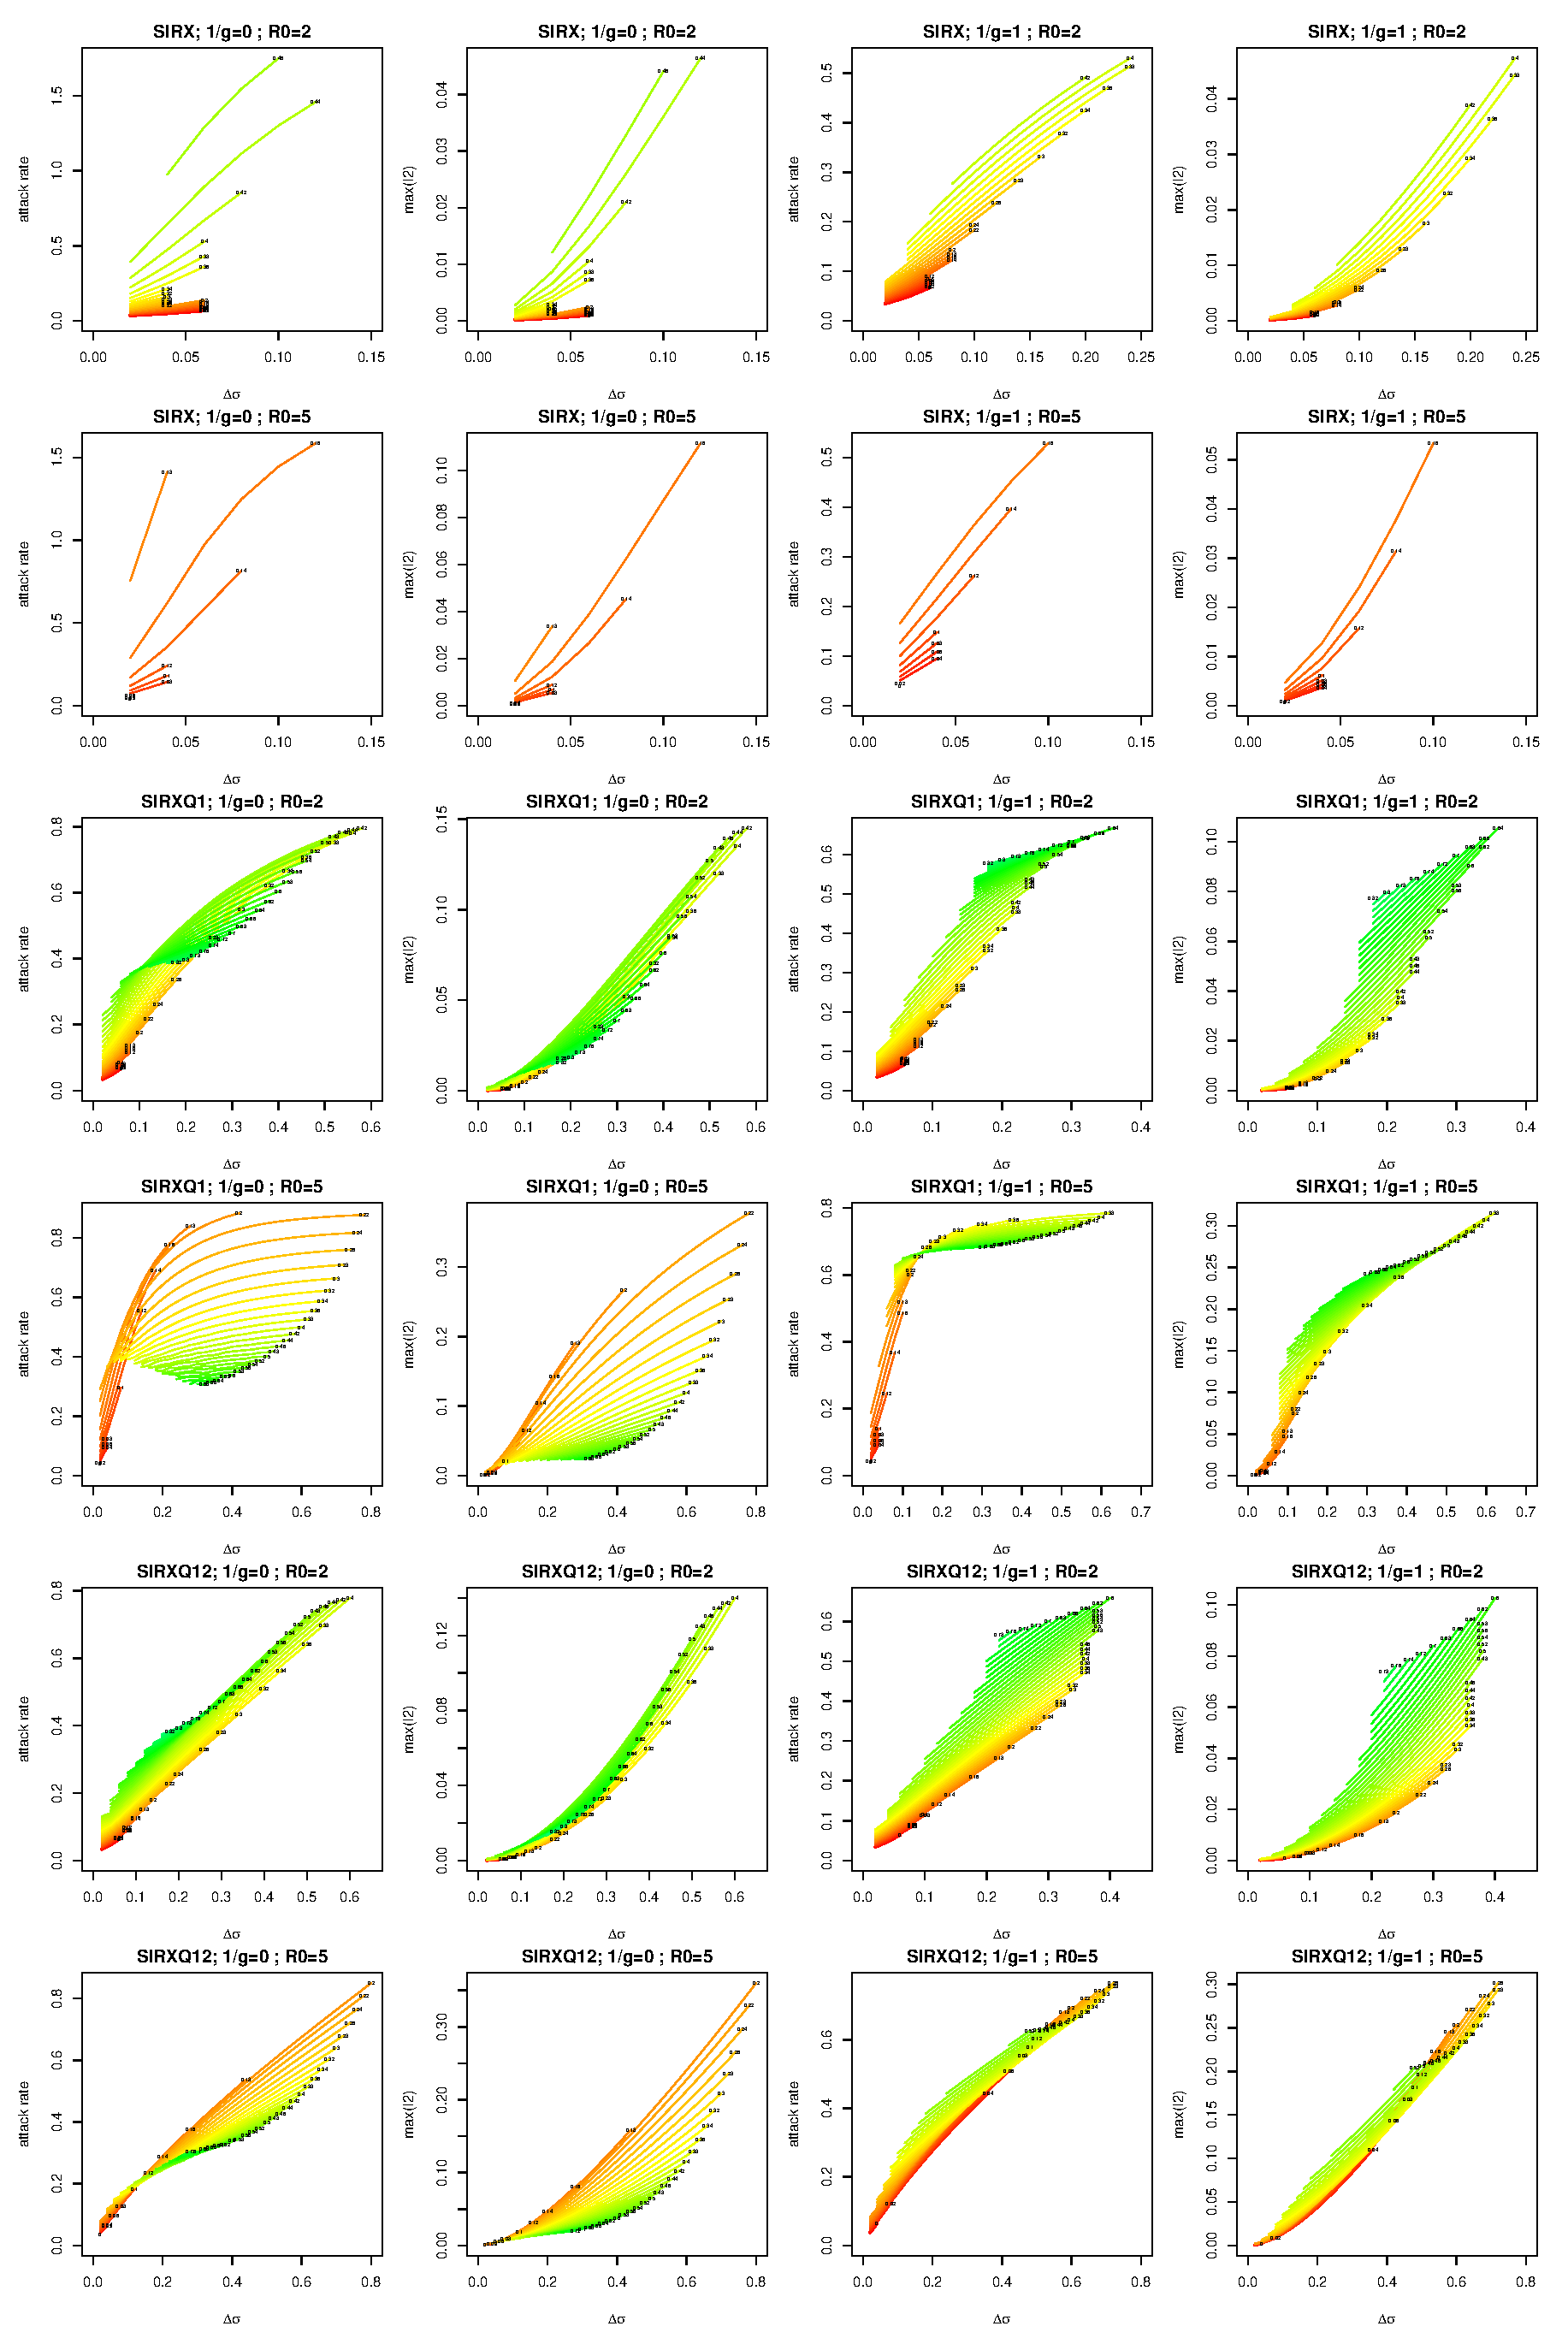
\includegraphics[width=0.8\linewidth]{texte/article3/appendix_diamond/graph/attak.eps}
  \caption{Effect of immune escape on the attack rate and the maximum
    epidemic size of the mutant antigenic unit for the $SIRX$ model
    (first and second lines), the $SIRXQ1$ model (third and fourth
    lines) and the $SIRXQ12$ model with immune boosting (fifth and sixth
    lines) in the parameter space where we expect replacement of the
    resident antigenic unit by the mutant one. Attack rate is
    calculated from the introduction time of the new antigenic unit to
    the first minimum of the epidemic curve. Immune escape is measure
    by $\Delta\sigma$.  Colors represent different values of
    $\sigma_X$ ensuring replacement. Parameters values are identical for
    both antigenic units ($\alpha=1$).}
  \label{fig:sirx_attak}
\end{figure}

\clearpage

\subsection{Effect of functional constraints}


\begin{figure}[!hp]
  \center
  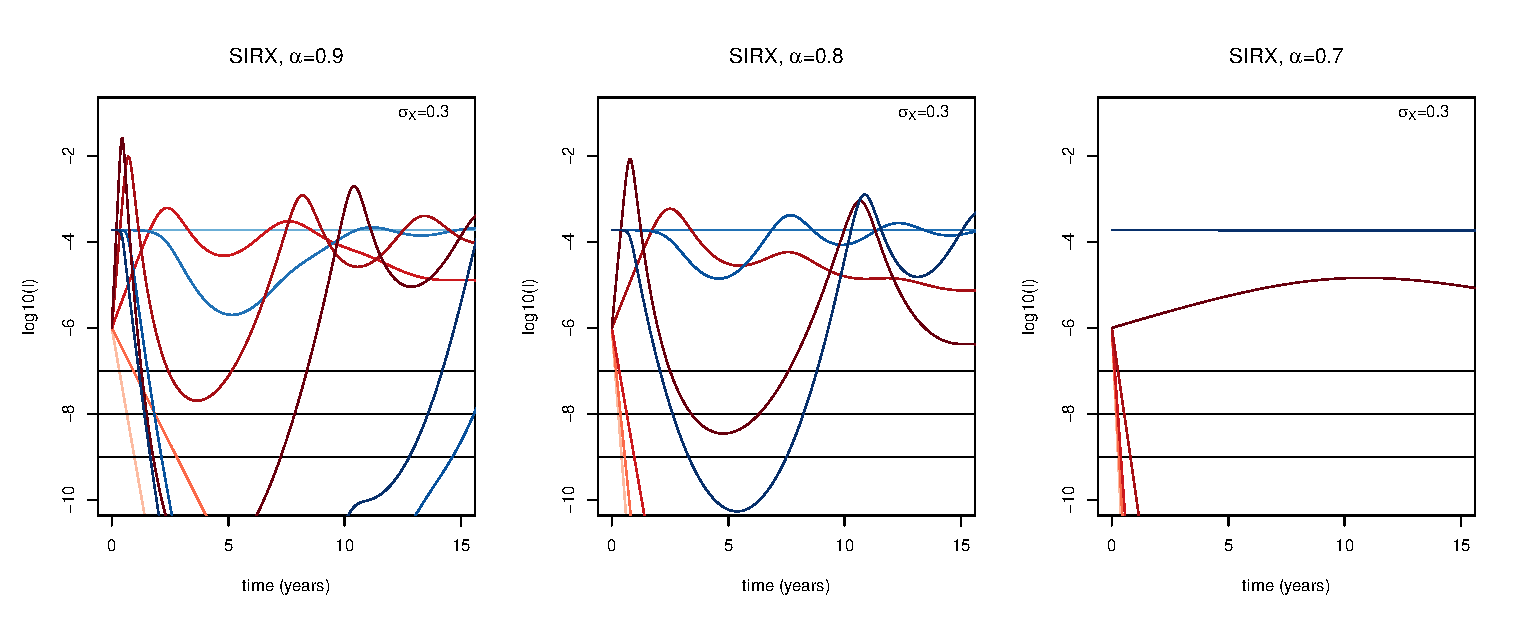
\includegraphics[width=0.9\linewidth]{texte/article3/appendix_diamond/graph/traj_deter_trade_off.eps}
  \caption{Effect of functional constraint on the invasion trajectory
    of a mutant antigenic unit introduced in a population where a
    resident antigenic unit is at the endemic equilibrium for the
    $SIRX$ model. Red and blue are prevalence of mutant and resident
    antigenic unit in log scale. Colours intensity indicates the
    degree of immune escape as measured by $\Delta\sigma$ (1\% (light
    tones); 5\%, 10\%, 20\% and 30\% (dark tones)). Parameters:
    $R_0=2$; $1/\nu=4$ days ; $1/g=1$ year ; $1/q=6$ months}
  \label{fig:traj_deter_trade_off}
\end{figure}

\clearpage

\subsection{Metapopulation dynamics: stochastic models}

\begin{figure}[!hp]
  \center
  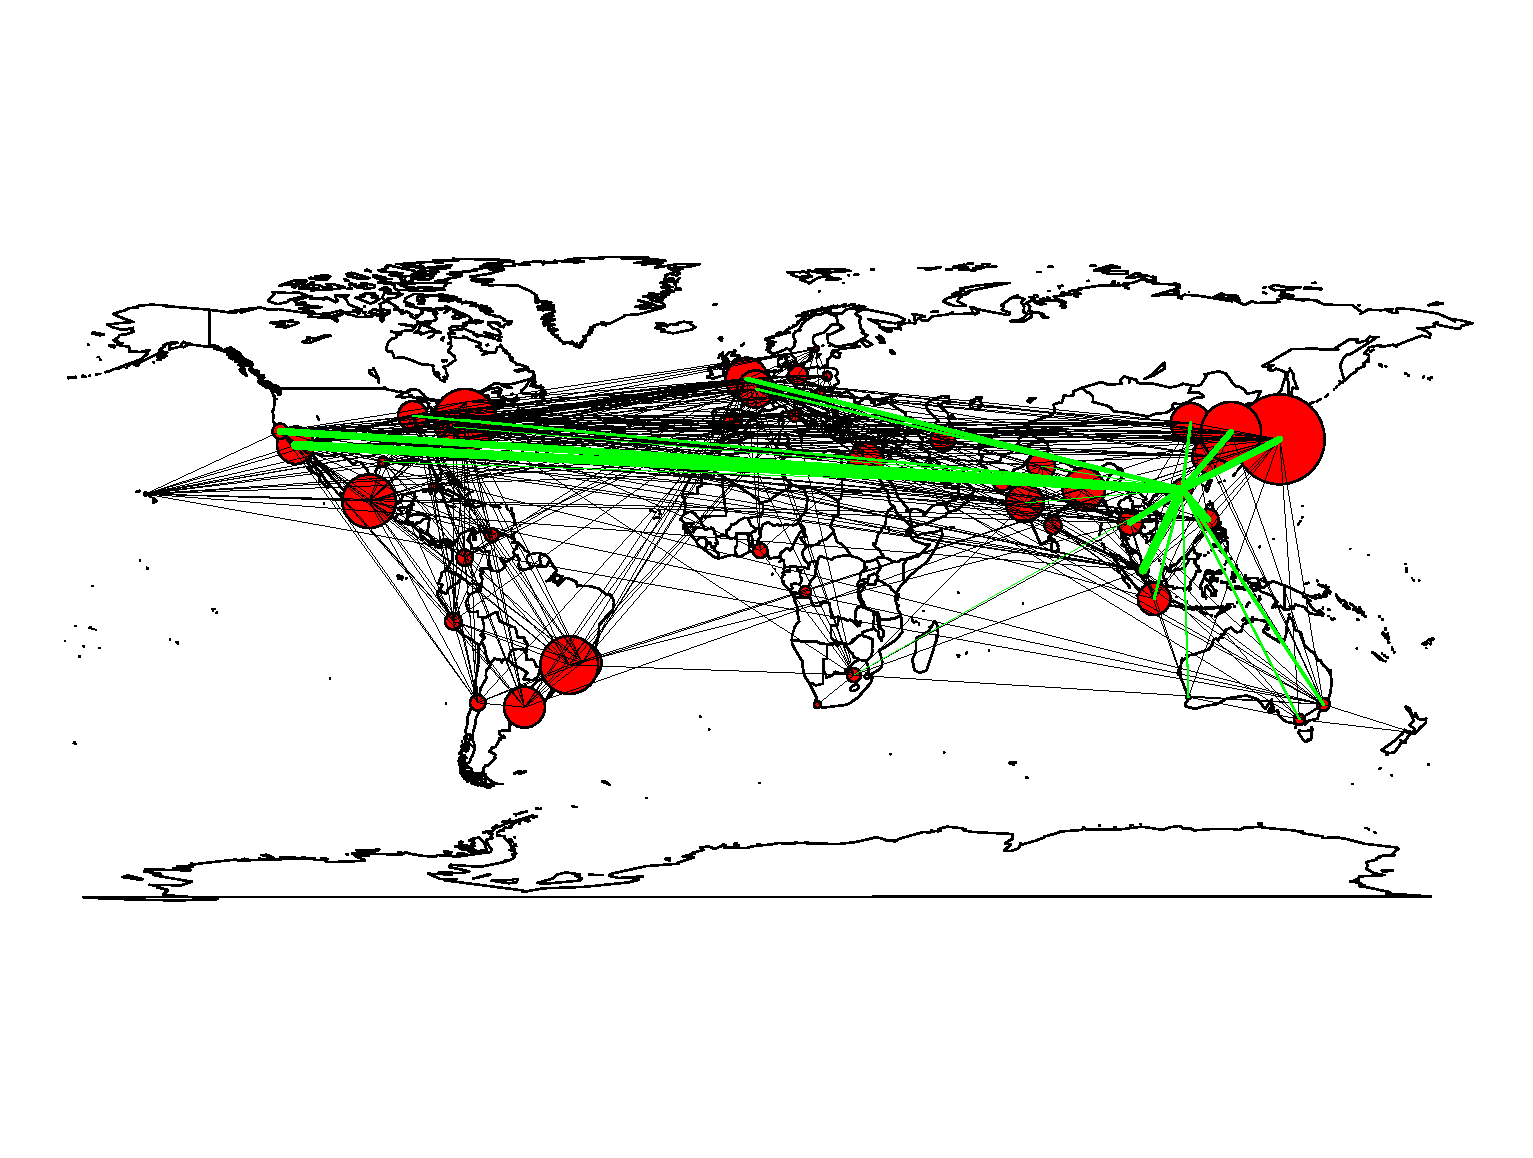
\includegraphics[width=0.6\linewidth]{texte/article3/appendix_diamond/graph/mapHK.eps}
  \caption{Overview of the network of 52 global cities used in the
    stochastic metapopulation model. Circle areas and lines width are
    proportionate to city sizes and air transportation flows. The
    mutant antigenic cluster is introduced in Shenzen. Shenzen air
    connections are indicated in green.}
  \label{fig:mapHK}
\end{figure}

\begin{figure}[!htbp]
  \center
  \includegraphics[width=0.8\linewidth]{texte/article3/appendix_diamond/graph/traj_metapop.eps}
  \caption{Typical realisation of the $SIRX$ (first panel) and
    $SIRXQ12$ with immune boosting (second panel) stochastic
    metapopulation models for the city of Paris. First antigenic unit
    is at the endemic equilibrium and the following antigenic units
    are introduced every 4 years in Shenzen on april 1$^{st}$ with an
    initial seed of 100 infected individuals. y-axis is weekly
    incidence per 100 000 inhabitants. Parameters: $\sigma_X=0.3$
    $\Delta\sigma\in\{0.01, 0.02, 0.05, 0.1\}$; $R_0=2$; $1/\nu=4$
    days ; $1/g=1$ year ; $1/q=6$. Vertical plain (dotted) lines are
    introduction (worldwide extinction) times of the antigenic units
    coded by colours. Corresponding annual attack rates are plotted in
    figure~\ref{fig:attack_rate_metapop}, and different realisations
    aggregated by geographics areas in
    figure~\ref{fig:aggreg_metapop}.}
  \label{fig:world_sirx}
\end{figure}



\begin{figure}[!hp]
  \center
  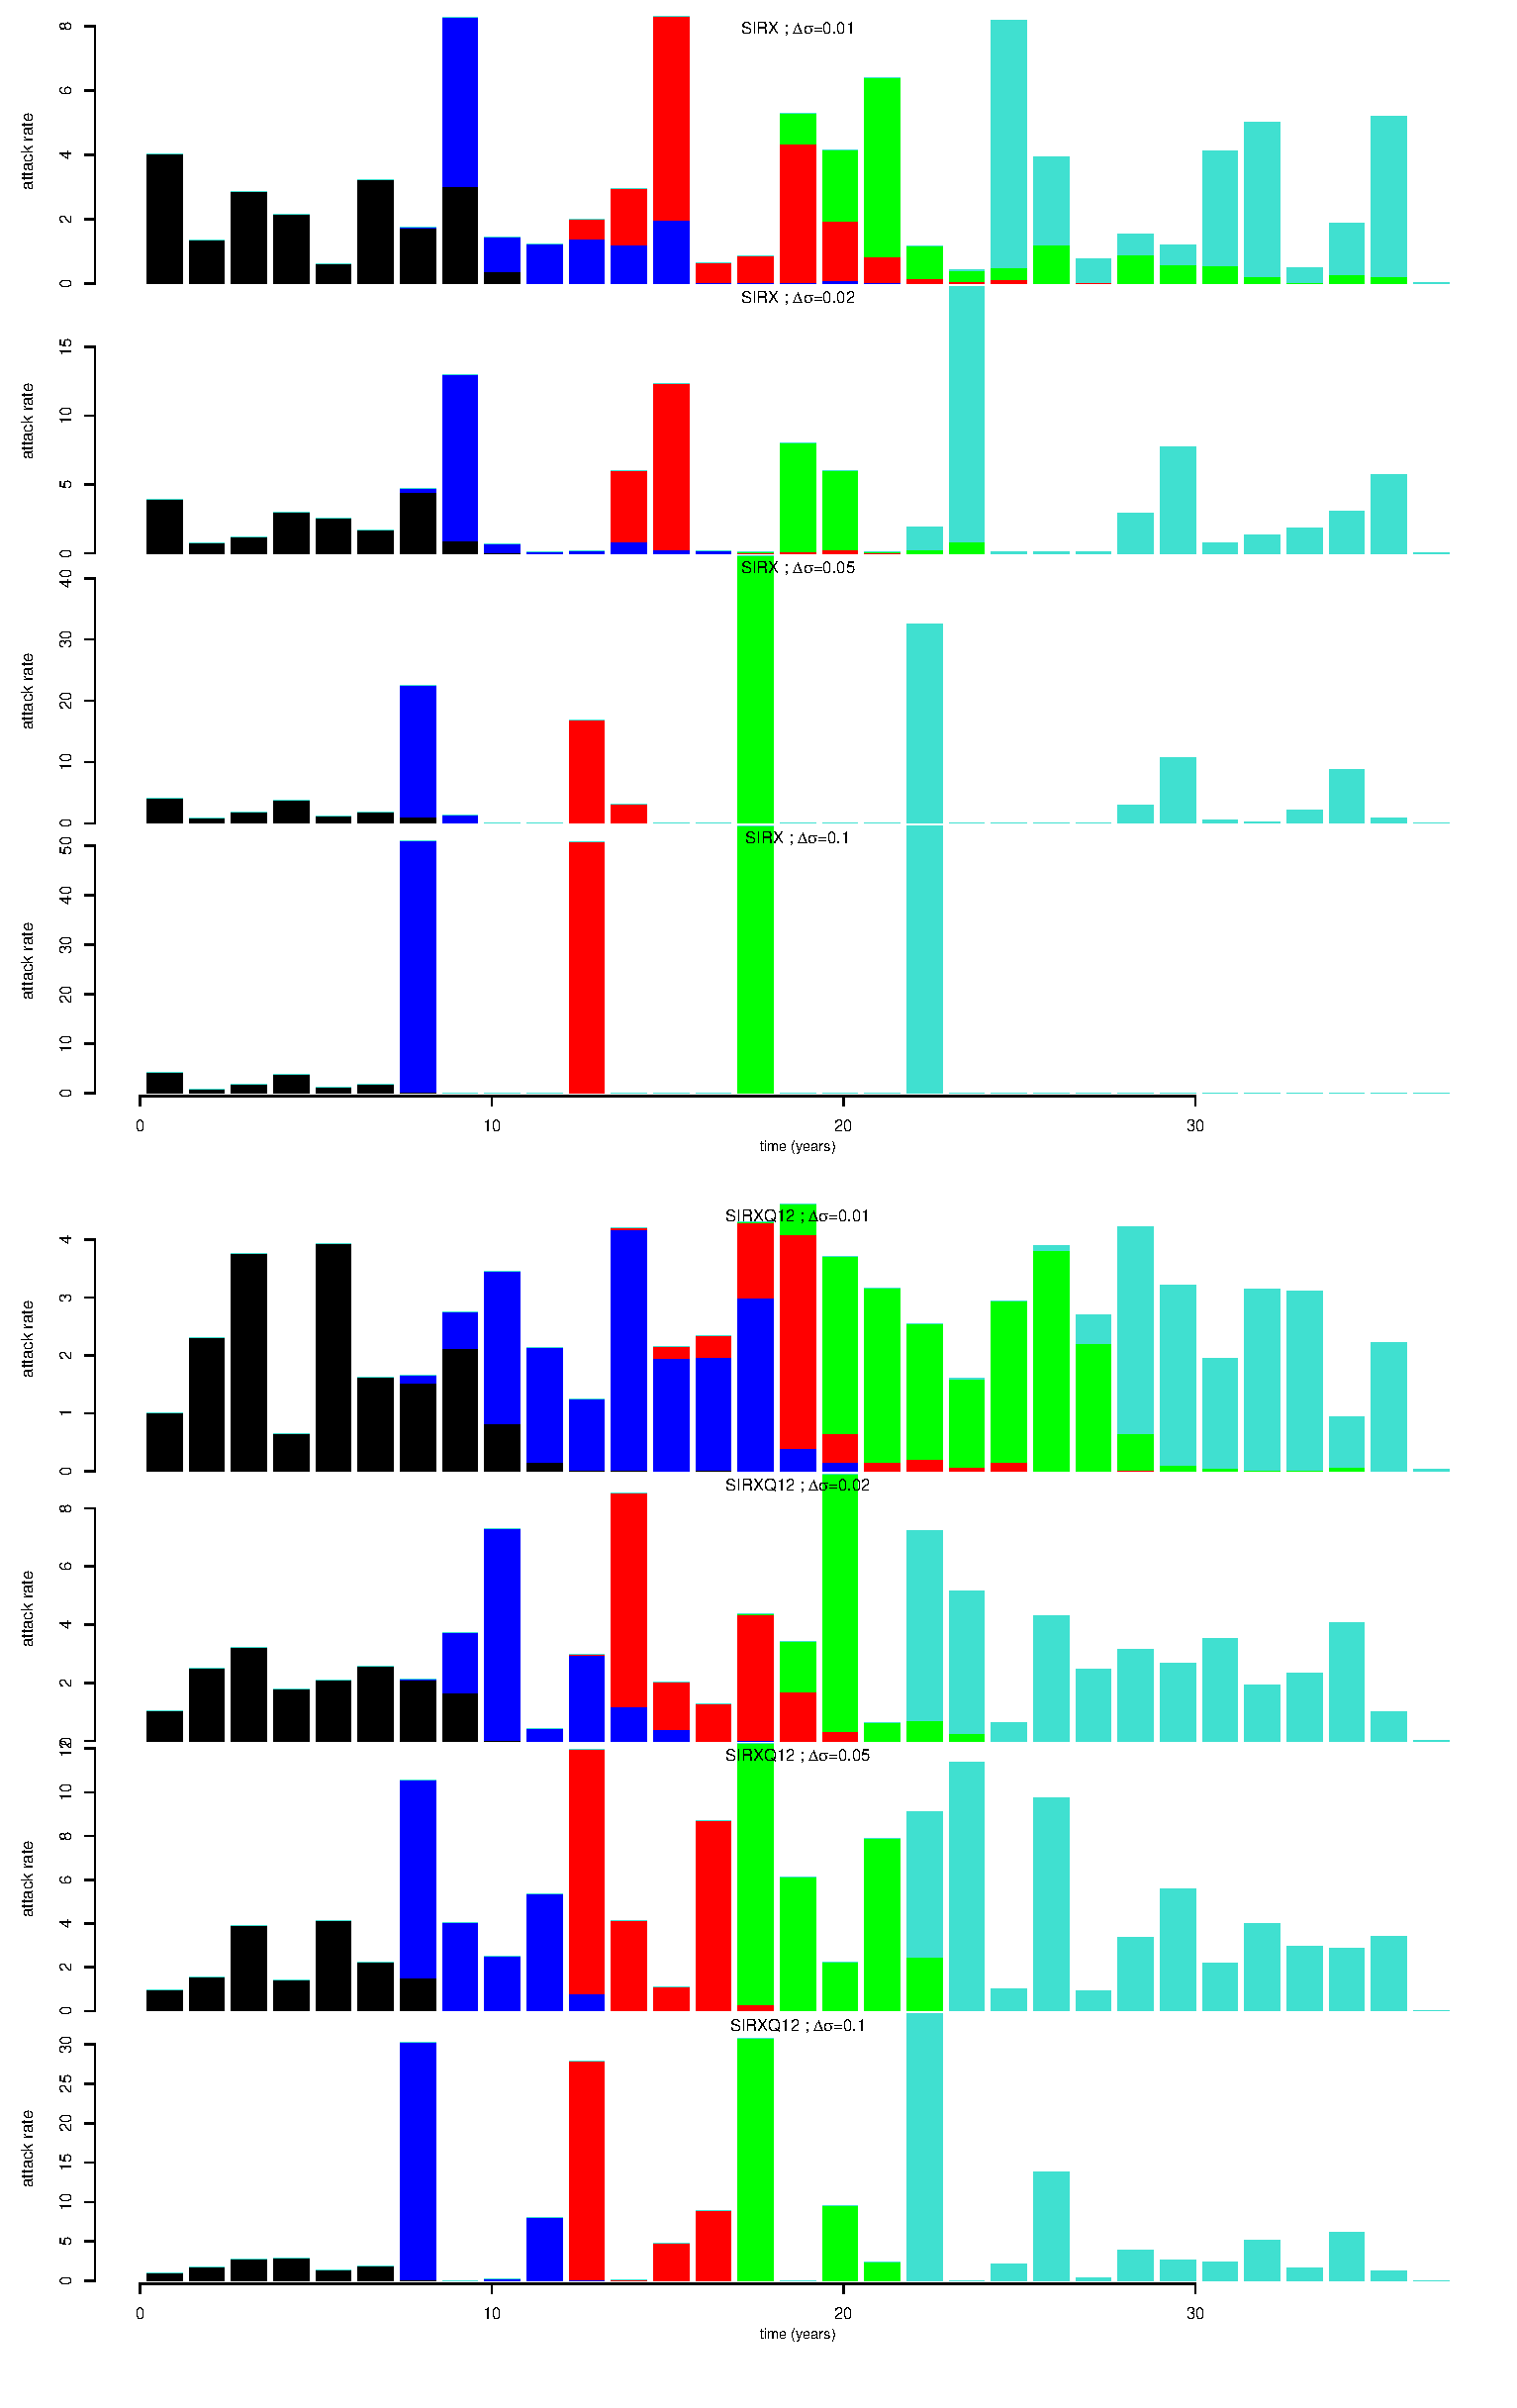
\includegraphics[width=0.9\linewidth]{texte/article3/appendix_diamond/graph/barplot.eps}
  \caption{Evolution of the annual attack rates in Paris for the
    realisations of figure~\ref{fig:world_sirx}.}
  \label{fig:attack_rate_metapop}
\end{figure}



\begin{figure}[!hp]
  \center
  \includegraphics[width=0.9\linewidth]{texte/article3/appendix_diamond/graph/traj5_sirx_siqrx_s03.eps}
  \caption{Trajectories for 20 realisations of the stochastic $SIRX$
    (first panel) and $SIRXQ12$ with immune boosting stochastic
    metapopulation models (second panel) aggregated by world
    areas. First, second and third columns are respectively North,
    Tropics and South. y-axis is weekly incidence per 100 000
    inhabitants. Parameters values are identical to
    figure~\ref{fig:world_sirx} with, for each panel immune escape
    ($\Delta\sigma$) intensities given from top to bottom by $0.01;
    0.02; 0.04; 0.1$. Vertical plain (dotted) lines are introduction
    (worldwide extinction) times of the antigenic units coded by
    colours.}
  \label{fig:aggreg_metapop}
\end{figure}


\begin{figure}[!hp]
  \center
  \includegraphics[width=0.9\linewidth]{texte/article3/appendix_diamond/graph/traj5_sirx_s039.eps}
  \caption{Trajectories for 20 realisations of the stochastic $SIRX$
    (first panel) and $SIRXQ12$ with immune boosting stochastic
    metapopulation models (second panel) aggregated by world
    areas. First, second and third columns are respectively North,
    Tropics and South.y-axis is weekly incidence per 100 000
    inhabitants. Parameters values: $\sigma_X=0.39$
    $\Delta\sigma=0.04$; $R_0=2$; $1/\nu=4$ days ; $1/g=1$ year ;
    $1/q=6$.}
  \label{fig:traj_sirx_s039}
\end{figure}


%\begin{figure}[!hp]
%%  \center
%%  \includegraphics[width=0.8\linewidth]{texte/article3/appendix_diamond/graph/image_sirx.eps}
%  \caption{Per city view of a realisation of the $SIRX$
%    metapopulation model. Black is the resident antigenic unit
%    and red the mutant one introduced in april 1$^{st}$ in
%    Shenzen. City are sorted by starting date of the muntant
%    antigenic unit epidemics and color coded by geographic
%    areas. Parameters values are identical to figure
%    \ref{fig:sirx_s03_039} with $\sigma_X=0.39$.}
%  \label{fig:cooper_sirx}
%\end{figure}
%
%
%\begin{figure}[!hp]
%%  \center
%%  \includegraphics[width=0.8\linewidth]{texte/article3/appendix_diamond/graph/image_siqrx_ferg.eps}
%  \caption{Per city view of a realisation of the $SIRX$
%    metapopulation model. Black is the resident antigenic unit
%    and red the mutant one introduced in april 1$^{st}$ in
%    Shenzen. City are sorted by starting date of the muntant
%    antigenic unit epidemics and color coded by geographic
%    areas. Parameters values are identical to figure
%    \ref{fig:sirx_s03_039} with $\sigma_X=0.39$.}
%  \label{fig:cooper_sirx}
%\end{figure}



%%% Local Variables: 
%%% mode: latex
%%% TeX-master: "../../../phD"
%%% End: 

%\cleardoublepage

\clearpage
\newpage
\thispagestyle{empty}
\null
\newpage

\definecolor{monVert}{RGB}{120,212,144}
%\tikzstyle{erlang} = [draw, fill=sectionColor, rectangle, minimum height=2em, minimum width=3em]
\tikzstyle{erlang} = [draw, fill=blue!20, rectangle, minimum height=2em, minimum width=3em]
%\tikzstyle{erlang_2} = [draw, fill=green!20, rectangle, minimum height=2em, minimum width=3em]
\tikzstyle{erlang_2} = [draw, fill=monVert, rectangle, minimum height=2em, minimum width=3em]
%\tikzstyle{expo} = [draw, fill=sectionColor, circle,minimum height=2em]
\tikzstyle{expo} = [draw, fill=blue!20, circle,minimum height=2em]
%\tikzstyle{expo_2} = [draw, fill=green!20, circle,minimum height=2em]
\tikzstyle{output} = [coordinate]
\tikzstyle{expo_2} = [draw, fill=monVert, circle,minimum height=2em]



\chapter{Reinfection as a potential phenomenon for influenza pandemics: Tristan da Cunha 1971 epidemic as a case study}


Anton Camacho;
Sébastien Ballesteros;
Bernard Cazelles 


\section{Introduction}

A swine-origin influenza A(H1N1) virus is responsible for the current
pandemic and reminds us that the risk of influenza pandemic is high
and will persist in the future. The lessons from the past are
therefore precious and may help us to anticipate and manage such
disasters. In this context the multiple-wave outbreaks of influenza
type A over one season, which have been reported during several
pandemic episodes of the past century, remain poorly understood. The
most striking example remains the ``Spanish'' influenza pandemic of
1918-1919 that occurred in three waves over 9 months, causing about 50
million deaths worldwide. As a result, successive attacks were
explicitly reported with individuals having experienced up to two
reinfection episodes over a short time interval
\citep{Health1920,Dudley1926,Mantle1973,Barry2008}.

Determining whether these multiple-wave epidemics were caused by the
same strain remains a challenge since there is few or even no virus
samples from each wave. However it is commonly believed that
apparition of new antigenically drifted variants escaping population
immunity takes years, which is inconsistent with the inter-wave
periods of few weeks \citep{Taubenberger2006}.

Although there is a lack of virological and serological analysis of
these epidemiological phenomena, mathematical models can provide
important insight into the underlying mechanisms that could explain
multiple-wave epidemics. These dynamics have been reproduced within
the simple epidemiological $SIR$ (Susceptible-Infectious-Removed)
framework by supposing that coinfection with other acute respiratory
infections increases the transmissibility of influenza virus
\citep{Merler2008} or by altering the structure of the network of
contacts in the course of the epidemic as a defensive behavioral
response \citep{Poletti2009}. However these models cannot explain
cases of multiple infections in the same host during a single epidemic
season. In contrast, \citet{Mathews2007} have introduced a flexible
model that allows for reinfection: following recovery from infection
hosts acquire protective immunity with a certain probability,
otherwise they become again susceptible. From its side,
\citet{Gomes2004} have invoked a partial immune protection for
explaining reinfection. Both mechanisms challenge the common
assumption that infection by an influenza strain confers life-long
protection against reinfection by the same strain \citep{Earn2002}.
Thus, explaining these epidemiological phenomena is not only of public
health policies interest but may also provide a better understanding
of the human immune response to a novel influenza virus.

In this work, we propose to disentangle between three different
biological mechanisms for explaining a two-wave influenza epidemic
with explicit cases of reinfection that occurred on the remote island
of Tristan da Cunha in 1971 and that was reported by
\citet{Mantle1973} (see also Figure \ref{fig:tdc}). This case is all
the more interesting that the small population remained fully isolated
all along the epidemic, ruling out the hypothesis of a second
influenza virus introduction from outside, and that serological
analysis confirmed the presence of influenza type A/H3N2 during both
waves \citep{Mantle1973}.

The emergence of new influenza strains will continue to pose
challenges to public health and to the scientific community. No one
can accurately predict the timing and severity of the next pandemic,
numerous key questions still remain unanswered. The influence of
multiple infections in a naive population is one of the uncertainties
that are critical for improving our understanding and for correctly
describing a given pandemic. Our approach is based on the analysis of
the shape and the timing of observed incidence time series in order to
compare stochastic models constructed with different
assumptions. Identification and comparison of models are achieved
through two recent plug-and-play frameworks perfectly adapted to
nonlinear stochastic models \citep{Ionides2006,Toni2009}. These
frameworks are based on the frequentist \citep{Ionides2006} or on the
bayesian \citep{Toni2009} philosophy and both allow for parameter
inference and model selection.

\begin{figure}
\begin{center}
\includegraphics[width=0.7\linewidth]{texte/tdc/graph/tdc.eps}
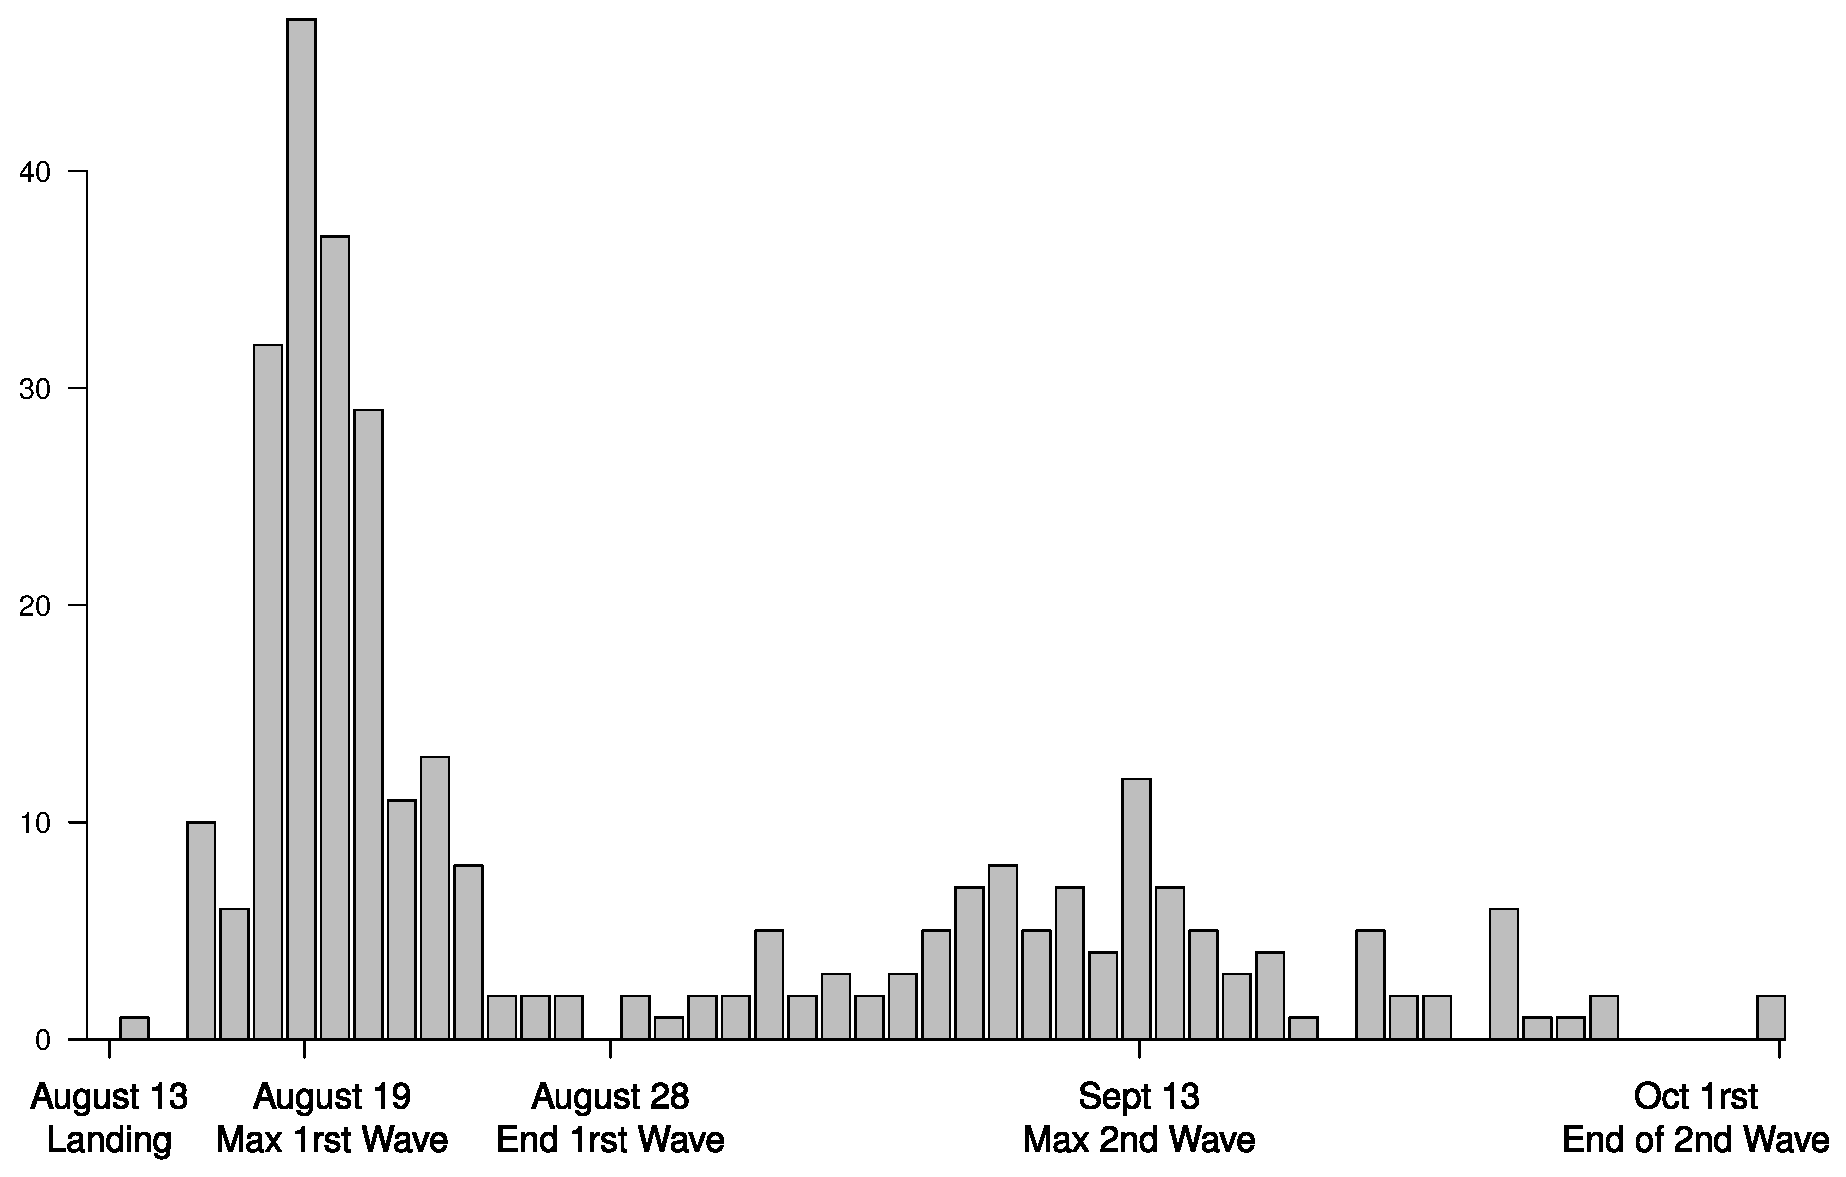
\includegraphics[width=0.7\linewidth]{texte/tdc/graph/data.eps}
\caption{Geographical position of Tristan da Cunha and incidence time series}
\label{fig:tdc}
\end{center}
\end{figure}


\section{Hypothesis Test}

Our aim was to explain the unusual influenza epidemic that occurred on
a small South-Atlantic island, named Tristan da Cunha, in 1971, 3
years after the emergence of new influenza A subtype H3N2. H3N2 was
introduced by a ship returning from Cape-Town that landed five
islanders on Tristan da Cunha. After the arrival of the ship an
influenza epidemic occurred over 50 days. But after three weeks of
propagation, while the epidemic was declining, some islanders
developed second attacks and a second peak of new cases was recorded
(see Figure \ref{fig:tdc}). Among the 284 islanders, 273 (96\%)
experienced at least one attack and 92 (32\%) experienced two attacks
(see \citet{Mantle1973} and \textsl{Material and Methods}).

Among all the explanations proposed to explain this two-wave epidemic,
\citet{Mantle1973} concluded that the hypothesis of reinfection by the
same viral agent was the only possible. However, they were unable to
determine if antigenic change in the virus have occurred, allowing for
second infection, or if some patients did not acquire an efficient
immune protection and were reinfected by other patients.
%
% (il y a aussi l'hyp de reinfection intra-hote)
%
Thus, the first biological hypothesis (subsequently referred as the
$MUT$ hypothesis) assumes that virus mutated within infected hosts
during the first epidemic-wave leading to the emergence of a new
antigenically drifted variant. However given that it normally takes
between 2 and 8 years at the scale of the global human population for
a new variant to acquire significant antigenic changes
\citep{Smith2004,Koelle2006} and since second attacks occurred only
three weeks after the beginning of the epidemic in a population of 284
individuals, we can reasonably assume that if a new variant emerged
during the first wave it had to happen within a single infected host.
The second biological hypothesis (subsequently referred as the $MI$
hypothesis) assumes that following recovery from infection some hosts
acquire a long-term protective immunity against reinfection whereas
some other become again fully susceptible to the virus. This
assumption was previously introduced by \citet{Mathews2007}. The third
hypothesis (subsequently referred as the $PP$ hypothesis) was
previously introduced by \citet{Gomes2004} and assumes that following
recovery from infection all hosts develop an immune response that is
not fully protective while reducing the risk of reinfection.

These 3 hypothesis have been translated into 3 different mathematical
models (see Figure \ref{fig:models_tdc} and \textsl{Materials and
  Methods}). Model parameters and their biological interpretation are
given in table \ref{tab1}. We used the stochastic framework for
running these 3 models. Parameter inference and model selection were
achieved through the plug-and-play framework proposed by
\citet{Ionides2006}. This frequentist approach converges to the maximum
likelihood parameter set estimate for each model and allows therefore
to compute the Akaike information criteria to select the model that
best explain the data (see \textsl{Material and Methods}).

\begin{center}
\begin{table}[htdp]
  \begin{footnotesize}
    \begin{tabular}{|l|l|c|c|c|}
      \hline
      Symbol & Description & $MUT$ & $MI$ & $PP$\\ \hline
      $R_{0}$ & basic reproductive number & 10.41 & 8.01 & 5.26 \\ \hline 
      $1/e$ & mean latent period (days) & 2.42 & 1.96 & 1.51 \\ \hline
      $1/v$ & mean infective period (days) & 1.20 & 1.39 & 0.87\\ \hline
      $1/g$ & mean temporary removed period (days) & 2.77 & 11.90 & 5.71\\ \hline
      $\alpha$ & probability to develop long-term immunity after infection & - & 0.48 &- \\ \hline
      1-$\sigma$ & partial protection induced by a first attack &0.83 &- & 0.78 \\ \hline
      $\rho$ & reporting rate for observation & 0.68 & 0.69 & 0.65 \\ \hline
      $T_{mut}$ & time of introduction of the new variant & $23^{rd}$ august &-&-\\ \hline
      $\mathcal{L}(\theta_{MLE})$ & Log-likelihood for each model &-130.03 & -106.13 & -124.11 \\ \hline
      $AIC_{c}$ & Akaike information criteria &279.41 & 231.61 & 267.57\\ \hline
    \end{tabular}
  \end{footnotesize}
\caption{Parameter description, maximum likelihood estimates and Akaike information criteria for each model}
\label{tab1}
\end{table}%
\end{center}

\begin{figure}
\begin{center}
\caption*{a) Mutation model ($MUT$)}
\label{MUT}
\begin{tikzpicture}[node distance=3cm, auto,>=latex', thick]
    %\path[use as bounding box] (-1,0) rectangle (10,-2);
    \path[->] node [expo] (sain) {S}
     	    node [erlang, right of=sain] (expose) {E1}
    node [erlang, right of=expose] (infecte) {I1}
    node [expo, right of=infecte] (immunise) {R1}
     (sain) edge node {$\beta$} (expose)
     (expose) edge node[name=e] {$e$}(infecte)
     (infecte) edge node{$v$}(immunise);
  
   \path[->]  node [erlang_2, below of=e] (infecte_2) {I2};
   %\path[->]  (infecte) edge[dashed] node{$\mathds{1}_{T_{mut}}$}(infecte_2);
    
         \path[->] node [erlang_2, right of=infecte_2] (expose_2) {E2}
    node [expo_2, left of=infecte_2] (immunise_2) {R2}
    
     
     (sain) edge node[near start,below] {$\beta$} (expose_2)   
     (infecte) edge node{$v$}(immunise) 	
     (immunise) edge node[near start] {$\sigma\beta$} (expose_2)
     (expose_2) edge node{$e$}(infecte_2)
     
     (infecte_2) edge node{$v$}(immunise_2);

\end{tikzpicture}


\vspace{0.5cm}
\caption*{b) Multiple-Infection model ($MI$)}
\begin{tikzpicture}[node distance=2cm, auto,>=latex', thick]

    % We need to set at bounding box first. Otherwise the diagram
    % will change position for each frame.
   % \path[use as bounding box] (-1,0) rectangle (10,-2);
     \node [expo] (sain) {S};
     	    \node [erlang, right of=sain] (expose) {E};
    \node [erlang, right of=expose] (infecte) {I};
    \node [erlang, right of=infecte] (immunise) {R};
    \node [expo, right of=immunise] (longue) {L};

% Once the nodes are placed, connecting them is easy. 
    \draw [->] (sain) -- node {$\beta$} (expose);
    \draw [->] (expose) -- node{$e$}(infecte);
    \draw [->] (infecte) -- node{$v$}(immunise);
    \draw [->] (immunise) -- node{$\alpha g$}(longue);
    \draw[->](immunise) -- +(0,1) -| node[near start,above] {$(1-\alpha)g$} (sain);
    
\end{tikzpicture}
%\label{MI}
\vspace{0.5cm}
\caption*{c) Partial-Protection model ($PP$)}
\begin{tikzpicture}[node distance=2cm, auto,>=latex', thick]
    % We need to set at bounding box first. Otherwise the diagram
    % will change position for each frame.
   % \path[use as bounding box] (-1,0) rectangle (10,-2);
     \node [expo] (sain) {S};
     	    \node [erlang, right of=sain] (expose) {E};
    \node [erlang, right of=expose] (infecte) {I};
    \node [erlang, right of=infecte] (immunise) {R};
    \node [expo, right of=immunise] (longue) {L};

% Once the nodes are placed, connecting them is easy. 
    \draw [->] (sain) -- node {$\beta$} (expose);
    \draw [->] (expose) -- node{$e$}(infecte);
    \draw [->] (infecte) -- node{$v$}(immunise);
    \draw [->] (immunise) -- node{$g$}(longue);
    \draw[->](longue) -- +(0,1) -| node[near start,above] {$\sigma\beta$} (expose);
    
\end{tikzpicture}
%\label{PP}
\end{center}
\caption{Three models with three different biological
  mechanisms. Square boxes stand for Erlang distribution for the
  residence durations into states $E$,$I$ and $R$ (shape $k=2$ and
  mean values $1/e$,$1/v$ and $1/g$). Circle boxes stand for simple
  exponential durations. Parameter description can be found in table
  \ref{tab1}.}
\label{fig:models_tdc}
\end{figure}


\section{Results}

Maximum likelihood estimate for the parameter set of each model is
presented in table \ref{tab1}. Estimates vary somewhat between models
and are characterized by a high $R_{0}$ ($> 5$), an infective period
of about one day and a latent period of about two days. Regarding the
$MI$ model estimate of $\alpha$ shows that in proportion about half of
the infected hosts did not develop a long-term protective immunity
after the first exposure. In contrast, for the $MUT$ and $PP$ models
estimates of the level of cross-protection conferred by the first
exposure is around 80\%. This discrepancy is however balanced by a
shorter temporary removed duration allowing hosts to be potentially
faster reinfected in both $PP$ and $MUT$ models than in the $MI$
model. The reporting rate ($\rho$) \textit{i.e.} the proportion of the
total cases that were reported, is estimated for all three models
around 70\%, which is under the minimal value of 85\% due to data
uncertainties (see \textsl{Material and Methods}). These parameter set
estimates are confirmed by the bayesian approach of \citet{Toni2009}
(see the supplementary document).

Figure \ref{res1} compares the average prediction of each model with
maximum likelihood parameter estimates. Whereas all three models
easily fit the first wave only the $MI$ model can capture the second
wave. This observation is statistically confirmed by the Akaike
information criteria which shows that the $MI$ model best explains the
data (see table \ref{tab1}). We also note that the $MUT$ model is the
least likelihood.

In order to understand why neither $PP$ nor $MUT$ models succeed to
capture the second wave epidemic (figure \ref{res1}) we calculated the
evolution of the extinction probability. Thus for all three models we
computed at each point in time the proportion of extinct simulations
over 100000 stochastic realizations. Results are shown on figure
\ref{res1} and point out the role of demographic
stochasticity. Indeed, whereas the extinction probability increases
rapidly at the end of the first wave for both $PP$ and $MUT$ models,
the $MI$ model appears to be much more robust to stochastic
extinctions during the inter-wave period. This conclusion is all the
more surprising that estimate of the temporary removed duration
($1/g$) is well above for the $MI$ model than for the other two.
Regarding the $MUT$ model, the sudden increase of the extinction
probability corresponds to a high risk of failed invasion for the
newly emerging variant in the population \citep{Lloyd-Smith2005}. The
case of the $PP$ model is more complicated. Previous analysis of a
similar but deterministic model \citep{Gomes2004,Gomes2005} have
revealed that dynamics are depending on a reinfection parameter
$\sigma R_{0}$. When this parameter is well above a reinfection
threshold \textit{i.e.} $\sigma R_{0}>1$, reinfection becomes
self-sustained and dynamics are $SIS$-like whereas below this
threshold primary infection dominates and leads to $SIR$-like
dynamics. Estimate for our stochastic $PP$ model gives $\sigma
R_{0}=1.3$ and indicates a critical dynamics: the reinfection
parameter needs to be sufficiently high to reduce stochastic
extinctions during the inter-wave period but in the same time it must
be sufficiently low to avoid sustained reinfection leading to more
than two epidemic waves. In other words the observed epidemic
extinction after the second wave decreases the reinfection parameter
and therefore increases the inter-wave extinction probability.

\begin{figure}
\includegraphics[width=0.9\linewidth]{texte/tdc/graph/res_et_extinction.eps}
\caption{Average prediction of each model with maximum likelihood parameter estimates}
\label{res1}
\end{figure}

\section{Discussion}

In this study we propose to use simple mathematical models to
disentangle between three biological mechanisms for explaining a
two-wave epidemic of influenza A/H3N2 on the island of Tristan da
Cunha in 1971. Following a model selection based on a rigorous
statistical framework \citep{Ionides2006}, we show that the most
likely explanation is that only 50\% of the patients developed a
long-lasting protection against the virus after the first attack
whereas unprotected hosts developed illness following re-exposure to
the same virus and initiated the second epidemic wave.

In a previous study \citet{Mathews2007} fitted a flexible model
(similar to our $MI$ model) on the same data set using a deterministic
framework. Their parameter estimate was achieved via MCMC but after
comparison of their mean estimate with our maximum likelihood estimate
we find very close values except for the mean serial interval
(infectious plus latent period), which is slightly greater in our
study (2.24 vs. 3.4 days). We think that this discrepancy is mainly
attributable to the incorporation of demographic stochasticity in our
approach: by fitting a deterministic model \citet{Mathews2007} neglect
the probability of stochastic extinction and implicitly underestimate
the duration of the serial interval which plays a significant role
during the inter-wave period. This remark emphasizes the need to use
stochastic simulations for parameter inference whenever the population
is low and/or demographic stochasticity is expected to play a
significant role \citep{Lloyd-Smith2005}.

Our estimates for the mean latent and infective periods of the $MI$
model are close to previous published estimates \citep{Cauchemez2004}
whereas the high value of the basic reproductive number is somewhat
unexpected for influenza virus since $R_{0}$ is usually estimated
around 2 \citep{Lessler2007}. However the rapid spreading of the virus
(the first peak was reached after 6 days only) as well as the
unusually high attack rate, which is typical of small isolated
communities \citep{Brown1966}, and the exceptional contact
configuration of the population of Tristan da Cunha
\citep{Samuels1963,Shibli1971} give support to such a high $R_{0}$
value \citep{Mathews2009}. Moreover, as we point out in the
\textsl{Material and Methods}, the single influenza virus most
islanders were exposed to before the epidemic of 1971 was a polyvalent
influenza vaccine dating from 1961 \citep{Tyrrell1967}. This vaccine
contained only an H2N2 strain and a B strain and it is unlikely to
have conferred protection against H3N2
\citep{Brown1969a,Brown1969b}. The high susceptibility of the
islanders to influenza contrasts with existing prior-immunity in
uninsulated communities and could contribute to the high estimated
value of $R_{0}$ \citep{McVernon2007,McCaw2009}.

The hypothesis of homogeneous mixing underlying the infection process
in our models may seem questionable even for the small population of
Tristan da Cunha \citep{Becker1983}. However it is a reasonable
assumption since topographical or sociological grouping
\citep{Shibli1971} are not expected to play a significant role on the
progress of the epidemic \citep{Hammond1971}.

From a more immunological stand point, human immune response to a
novel antigen/virus remains poorly understood in the case of influenza
although it is of first importance for managing a new pandemic
\citep{Doherty2006}. This response varies among individuals and
previous works have argued that such variability could depend on two
factors: the way the antigen/virus is introduced into the organism and
the immune history of the infected host. Indeed, it is commonly
admitted that a single natural infection by an influenza strain
confers life-long immunity against this strain whereas two vaccine
injections may usually be necessary to guarantee protection.
% (ref?)
%
Regarding the immune history, hosts with prior exposure and
pre-existent antibodies to several influenza strains have usually a
better response to vaccination \citep{Brown1969a} although it has also
been reported that these hosts could suffer from an original antigenic
sin \textit{i.e.} infection by a new influenza variant induces a
strong recall of antibodies against previously encountered antigens
but a weak immune response against the novel antigens \citep{Kim2009}.

Nevertheless the original antigenic sin mechanism may not have been
involved in the lack of immune response for 50\% of the population of
Tristan da Cunha since the level of prior-exposure to influenza virus
was unusually low in this population. Moreover, previous studies of
isolated naive communities have shown evidences for high specific
immune response following natural infection
\citep{Brown1966,Brown1969a,Brown1969b}.
%(confirmer, par ailleurs lors d'un antigenic sin on peut quand me gur
%de la premie attaque?).

Generally, isolated communities are expected to be less exposed, and
then more susceptible, to many diseases otherwise commonly encountered
in uninsulated populations. This obvious fact was confirmed for the
population of Tristan da Cunha after its evacuation due to a volcano
eruption in 1961. It was then reported that most adults suffered from
children diseases during their 2-year stay in Great-Britain
\citep{Tyrrell1967}. Thus, regarding influenza, the naive population
of Tristan da Cunha can reasonably be considered immunologically
closer to child than to adults of uninsulated communities before the
A/H3N2 epidemic of 1971.

Among the studies that have reported explicit cases of reinfection
during pandemic or inter-pandemic seasons, some presented significant
differences between children and adults the former being less
protected than the latter \citep{McVernon2007}. For example,
\citet{FOX1982a,FOX1982b} reported cases of reinfection by H3N2 during
the period of 1975-1979 in Seattle families. Their serological
analysis revealed that in those under (resp. above) age 20 years 36\%
(resp. 24\%) were reinfected, 75\% (resp. 17\%) of whom developed
illness. By comparing the HI titers of the two groups they found that
high titers $(\geqslant 1:40)$ were conferring protection against
illness only in the above 20 year age group.
% only the adults with low titers (<1:40) developed illness after reinfection whereas in the under 20 year age group high titers conferred no protection against illness.

Whereas the study of \citeauthor{FOX1982a} was conduced during an
inter-pandemic episode and over a much larger time scale than in our
case-study, the reported infection pattern of the under 20 year age
group seems very comparable to the one observed in the population of
Tristan da Cunha.

%This last remark calls for careful surveillance of naive populations such as the younger during pandemic episodes since even after a first attack these populations could be reinfected and keep the spread of the epidemic. 


On the other hand, even if it is not straightforward to compare
vaccination with natural infection, vaccination experiments during
past influenza pandemic tend also to support the idea that multiple
infections in immunologically naive hosts are needed before mounting a
protective immune response. For instance, whereas a single injection
of H1N1 vaccine was giving as good response as two injections prior to
1957, the advent of H2N2 pandemic in 1957 changed the situation since
two injections became necessary to confer protection
\citep{HOLLAND1958}.  The re-introduction of H1N1 in 1977-1978 also
offers an interesting case study as two injections of vaccine were
more effective than a single injection for children and young adults
whereas less difference was detected in hosts infected with H1N1 at
least 20 years earlier \citep{Nicholson1979}.


In conclusion, the importance of the present analysis is to highlight
the influence of reinfection in an influenza epidemic that occurred in
the unusually well-documented population of Tristan da Cunha. Our
results suggest that some people need multiple exposures to the virus
before developing a sufficiently immunological response and a
protective immunological memory. These historical data alone cannot
prove the importance of reinfection and immunological maturation in
influenza epidemics in a naive population nevertheless our findings
suggest that it may play a non-negligible role and call for careful
surveillance of naive populations, such as the youths, during pandemic
episodes since even after a first attack these populations could be
reinfected and keep the spread of the virus.


\section{Materials and Methods}

\subsection{Data}

Tristan da Cunha is a volcanic island in the South Atlantic Ocean. It
has been inhabited since the $19^{th}$ century and in 1971, the 284
islanders and 20 expatriates were living in the single village of the
island: Edinburgh of the Seven Seas (\citet{Samuels1963}, Figure
\ref{fig:tdc}). Whereas the internal contacts were typical of
well-knit village communities, contacts with the outside world were
infrequent and mostly due to fishing vessels that occasionally were
taking passengers to or from the island. These ships were often the
cause of introduction of new diseases on the population. Focusing on
influenza, several serological analysis between 1955 and 1963 provide
important insight into the immune status of the 284 islanders before
1971. Following an epidemic of H1N1 in 1954 during which most of the
islanders were infected, antibodies to older influenza A and B types
were detected in islanders over 20 years of age
\citep{Taylor-Robinson1963}. In 1961 when the volcano erupted the
island was evacuated to Britain via Cape-Town and the islanders were
given a polyvalent influenza vaccine that contained an H2N2 strain and
a recent B strain. Antibody studies showed a good response to this
inoculation \citep{Tyrrell1967}. Since the population returned to
Tristan da Cunha in 1963, no influenza epidemic has been reported. In
this context of a small population with weak and homogenous immune
repertoire against influenza virus, an unusual epidemic occurred in
1971, 3 years after the emergence of new subtype H3N2.

On august $13^{th}$, a ship returning from Cape-Town landed five
islanders on Tristan da Cunha. Three of them developed acute
respiratory disease during the 8-day voyage and the other two
presented similar symptoms immediately after landing. Various family
gatherings welcomed their disembarkation and in the next day epidemic
started to spread rapidly throughout the whole island
population. After three weeks of propagation, while the epidemic was
declining, some islanders developed second attacks and a second peak
of new cases was recorded. The epidemic fade out after this second
wave and lasted a total of fifty days.

Among the 284 islanders, 273 (96\%) experienced at least one attack
and 92 (32\%, mainly adults) experienced two attacks. Only few
individuals experienced their single attack during the second epidemic
wave. Unfortunately, only 312 of the 365 attacks (85\%) are known
within a single day accuracy and constitute the data set
\citep{Mathews2007}. These uncertainties can nevertheless be managed
since the statistical framework of \citet{Ionides2006} allows for
measurement errors. A precise description of the clinical features of
the illness as well as a review of the secondary infections were
provided by \citet{Mantle1973}. They reported that 85\% of the first
attacks were moderate or severe and this proportion decreased to 50\%
for the second attacks. However, they noted that 21 individuals
experienced two severe attacks. Serological analysis of infected
individuals demonstrated a high level of antibody against H3N2, a
subtype the population was never exposed to. Moreover, this high level
was detectable in individuals infected only during the first or the
second epidemic wave, attesting that the virus was circulating
throughout the epidemic. Unfortunately, no virological analysis were
conducted to show whether first and second attacks were due to
antigenically differing strains of H3N2.

\subsection{Models}

We model the three hypotheses via three simple mechanistic models
(Figure \ref{fig:models_tdc}). All the models use the same infection
process: after exposure to influenza virus susceptible hosts ($S$)
pass through a latent state ($E$) before becoming infectious
($I$). Infectious hosts enter the removed state ($R$) when they are
temporary unable to participate to the epidemic spreading: this may be
due to quarantine in bed or to temporary full-immunity because of
cell-mediated protection. Time spent in the $E$,$I$ and $R$ classes
follows an Erlang distribution with shape equal to 2 allowing for a
larger, more realistic, variance than the exponential
distribution. Note also that while in class $R$ hosts are protected
against reinfection.
 
The first model corresponds to the emergence of a new variant by
Mutation (labeled $MUT$). It is implemented by a history-based
2-strains model. The new variant is introduced at a single point of
time when an infectious host with strain 1 becomes infectious with
strain 2 (for simplicity, co-infection is not allowed). Both strains
are supposed to have the same transmissibility and to cross-react
\textit{i.e.} following infection by a single strain, as hosts leave
the removed class $R$ to enter the class $L$ they benefit a reduction
of susceptibility $\sigma$ against infection by the other strain.

The second model corresponds to the assumption that some hosts need
Multiple Infection before acquiring a long-term immunity (labeled
$MI$). When leaving the temporary removed state ($R$), each host has a
probability $\alpha$ to develop a long-term protection against
reinfection entering class $L$, otherwise host becomes again fully
susceptible to the virus and re-enter class $S$.

The third model corresponds to the assumption that long-term immunity
is always developed after infection while only Partially Protective
against reinfection (labeled $PP$). When leaving the temporary removed
state ($R$), each host enters the long-term immunity class $L$ and
benefit a reduction of susceptibility $\sigma$ against reinfection.

\subsection{Simulation and model selection} 


Given the small population of Tristan da Cunha demographic
stochasticity is expected to play a significant role in the epidemic
dynamics, especially during the inter-wave period when the number of
infected hosts is low and epidemic fade-out is likely to happen. We
therefore used the stochastic framework of continuous-time Markov
processes that naturally allows to take demographic stochasticity into
account.

Identification and model comparison have been performed with a
plug-and-play framework perfectly adapted to nonlinear stochastic
models \citep{Ionides2006,Breto2009,Toni2009}. In this paper we choose
to use the frequentist framework of iterated filtering
\citep{Ionides2006,King2008} due to its computational efficiency. In
addition we have confirmed the parameter inference for all models via
the bayesian approach of \citet{Toni2009}.

Numerical simulations were performed using the exact algorithm
provided by \citet{Gillespie1977}. Model predicted incidence is
computed by counting the daily number of new hosts entering the
infectious class $I$. Since the data set reports only 85\% of the
total number of attacks and in order to take into account measurement
errors, the observation process must also be modeled. We use a Poisson
process observation whose reporting rate parameter ($\rho$) is also
inferred \citep{Ionides2006,Breto2009}. Thus, we fitted each model to
infer the parameter set that maximizes the likelihood. Convergence to
the maximum likelihood was checked by computing profile likelihood
(see the supplementary document). These parameter sets were used to
simulate the average prediction of each model over 100000 runs and we
computed the corresponding likelihood. Finally we used the Akaike
information criteria to select the model that best explain the data:
$AIC_c=-2\mathcal{L}(\theta_{MLE})+2k+\frac{2k(k+1)}{n-k-1}$ where $k$
is the number of parameters and $n$ is the number of observations.



%%% Local Variables: 
%%% mode: latex
%%% TeX-master: "../../phD"
%%% End: 




\clearpage
\newpage
\thispagestyle{empty}
\null
\newpage


%\cleardoublepage
%\newpage
\bibliographystyle{apalike-fr}
\bibliography{/home/seb/Documents/biblio_bibtex/biblio_seb}

\end{document}


%%% Local Variables: 
%%% mode: latex
%%% TeX-master: t
%%% End: 
